\documentclass[11pt,a4paper]{book}
\pdfinclusioncopyfonts=1
\usepackage{lmodern}
\usepackage[nottoc]{tocbibind}
\usepackage{morewrites}
\usepackage{color,soul}
\usepackage{mwe}
\usepackage{hhline}
%\usepackage{algorithm}
\usepackage[svgnames]{xcolor}	
\usepackage[ruled,vlined]{algorithm2e}
\usepackage{algpseudocode}
\usepackage{tikz}
\usepackage{emptypage}
\usepackage{float}

\usepackage{color}
\definecolor{gray90}{gray}{.90}
\definecolor{gray75}{gray}{.75}
\definecolor{gray45}{gray}{.45}
\usepackage{listings}
\lstset{ frame=Ltb,
framerule=0pt,
aboveskip=0.5cm,
framextopmargin=3pt,
framexbottommargin=3pt,
framexleftmargin=0.4cm,
framesep=0pt,
rulesep=.4pt,
backgroundcolor=\color{gray90},
rulesepcolor=\color{black},
%
stringstyle=\ttfamily,
showstringspaces = false,
basicstyle=\small\ttfamily,
commentstyle=\color{gray45},
keywordstyle=\bfseries,
%
numbers=left,
numbersep=15pt,
numberstyle=\tiny,
numberfirstline = false,
breaklines=true,
}

% minimizar fragmentado de listados
\lstnewenvironment{listing}[1][]
{\lstset{#1}\pagebreak[0]}{\pagebreak[0]}

\lstdefinestyle{consola}
{basicstyle=\scriptsize\bf\ttfamily,
backgroundcolor=\color{gray90},
}

\lstdefinestyle{C}
{language=C,
}

% PAQUETES PARA MOSTRAR EL .CONFIG
\usepackage{listings}
\usepackage{xcolor}

\colorlet{punct}{red!60!black}
\definecolor{background}{HTML}{EEEEEE}
\definecolor{delim}{RGB}{20,105,176}
\colorlet{Mycolor1}{green!10!orange!90!}
\colorlet{numb}{magenta!60!black}


\lstdefinelanguage{config}{
    comment=[l]{//},
    commentstyle=\color{gray},
    string=[s]{"}{"},
    stringstyle=\color{blue},
    emph={SIGMOID, true, false},
    emphstyle={\color{Green}},
    basicstyle=\scriptsize,
    numbers=left,
    numberstyle=\scriptsize,
    stepnumber=1,
    numbersep=8pt,
    showstringspaces=false,
    breaklines=true,
    frame=lines,
    backgroundcolor=\color{background},
    literate=
     *{0}{{{\color{numb}0}}}{1}
      {1}{{{\color{numb}1}}}{1}
      {2}{{{\color{numb}2}}}{1}
      {3}{{{\color{numb}3}}}{1}
      {4}{{{\color{numb}4}}}{1}
      {5}{{{\color{numb}5}}}{1}
      {6}{{{\color{numb}6}}}{1}
      {7}{{{\color{numb}7}}}{1}
      {8}{{{\color{numb}8}}}{1}
      {9}{{{\color{numb}9}}}{1}
      {:}{{{\color{punct}{:}}}}{1}
      {,}{{{\color{punct}{,}}}}{1}
      {\{}{{{\color{delim}{\{}}}}{1}
      {\}}{{{\color{delim}{\}}}}}{1}
      {[}{{{\color{delim}{[}}}}{1}
      {]}{{{\color{delim}{]}}}}{1}
      {á}{{\'a}}1 {é}{{\'e}}1 {í}{{\'i}}1 {ó}{{\'o}}1 {ú}{{\'u}}1
      {Á}{{\'A}}1 {É}{{\'E}}1 {Í}{{\'I}}1 {Ó}{{\'O}}1 {Ú}{{\'U}}1
      {à}{{\`a}}1 {è}{{\`e}}1 {ì}{{\`i}}1 {ò}{{\`o}}1 {ù}{{\`u}}1
      {À}{{\`A}}1 {È}{{\'E}}1 {Ì}{{\`I}}1 {Ò}{{\`O}}1 {Ù}{{\`U}}1
      {ä}{{\"a}}1 {ë}{{\"e}}1 {ï}{{\"i}}1 {ö}{{\"o}}1 {ü}{{\"u}}1
      {Ä}{{\"A}}1 {Ë}{{\"E}}1 {Ï}{{\"I}}1 {Ö}{{\"O}}1 {Ü}{{\"U}}1
      {â}{{\^a}}1 {ê}{{\^e}}1 {î}{{\^i}}1 {ô}{{\^o}}1 {û}{{\^u}}1
      {Â}{{\^A}}1 {Ê}{{\^E}}1 {Î}{{\^I}}1 {Ô}{{\^O}}1 {Û}{{\^U}}1
      {œ}{{\oe}}1 {Œ}{{\OE}}1 {æ}{{\ae}}1 {Æ}{{\AE}}1 {ß}{{\ss}}1
      {ű}{{\H{u}}}1 {Ű}{{\H{U}}}1 {ő}{{\H{o}}}1 {Ő}{{\H{O}}}1
      {ç}{{\c c}}1 {Ç}{{\c C}}1 {ø}{{\o}}1 {å}{{\r a}}1 {Å}{{\r A}}1
      {€}{{\EUR}}1 {£}{{\pounds}}1,
}


\usepackage{multirow}
\usepackage{graphicx}
\usepackage{preview}
\usepackage{datatool}
\usepackage{setspace}
\usepackage{caption}
\usepackage[utf8]{inputenc}
\usepackage[spanish]{babel}


\usepackage{eqnarray}
\usepackage{preview}
\usepackage{datatool}
\usepackage{setspace}
\usepackage{caption}

\usepackage{latexsym}	
%\usepackage[T1]{fontenc}
\usepackage{amsfonts}
\usepackage{amsmath}%\usepackage[reqno]{amsmath}
\usepackage{rotating}
\usepackage{url}
%\usepackage{breakurl}
\usepackage{proof}
\usepackage{alltt}
\usepackage{multirow}
\usepackage{multibib}
\newcites{rec}{Bibliograf\'ia}
\usepackage{colortbl}
\usepackage[none]{hyphenat}

%\usepackage{indentfirst}

\usepackage{enumerate}
%\usepackage[colorlinks=true, pdfstartview=FitV, linkcolor=black, citecolor=black, urlcolor=black]{hyperref} %descomentar en la version de imprimir

\usepackage[colorlinks=true, pdfstartview=FitV, linkcolor=blue, citecolor=blue, urlcolor=blue]{hyperref} %comentar en la version de imprimir
\usepackage{verbatim}
\usepackage{amssymb}
%\usepackage{etex}
%\usepackage{hetcasl}
%\usepackage{algorithm}
%\usepackage{algorithm2e}
\usepackage{pdflscape}
\usepackage{lscape}
\usepackage{longtable}
%\usepackage{tocbibind}
\usepackage{booktabs}
%\usepackage{auto-pst-pdf}
\usepackage{graphicx}
\usepackage{psfrag}
%\usepackage{xypic}
\usepackage{pst-all}
\usepackage{comment}
\usepackage{indentfirst}
\usepackage[a4paper]{geometry}
\usepackage{rotating}
\usepackage{tabularx}
\usepackage{array}
\usepackage{subfigure}
\usepackage[nopostdot,nonumberlist,shortcuts,acronym,toc]{glossaries}

\hyphenation{con-fi-gu-ra-ciones}
\hyphenation{eli-mina}
\hyphenation{va-rie-dad}
\hyphenation{ma-ne-ra}
\hyphenation{dis-po-si-ti-vos}
\hyphenation{des-co-no-ci-do}

\makenoidxglossaries

\usepackage[vlined]{algorithm2e}%\usepackage[lined,boxed,commentsnumbered]{algorithm2e}
\usepackage{appendix}
\usepackage{dashrule}
\usepackage{verbatim} % comentarios
 %\usepackage{soulpos} 
%\usepackage[author={Ana}]{pdfcomment}
\makenoidxglossaries
%\RequirePackage{etex}
\usepackage[ruled,vlined]{algorithm2e}
\usepackage{algpseudocode}
\usepackage{tikz}
\newcommand*\circled[1]{\tikz[baseline=(char.base)]{\node[shape=circle,fill=blue!20,draw,inner sep=1pt] (char) {#1};}}
%\newcommand*\circled[1]{\tikz[baseline=(char.base)]{\node[shape=circle,draw,inner sep=1pt] (char) {#1};}}
\renewcommand{\algorithmicforall}{\textbf{for each}}


\geometry{a4paper}
\geometry{top=3cm,bottom=3cm,left=3cm,right=3cm,headsep=1cm}
%\renewcommand{\baselinestretch}{1.25}
%\setlength{\parskip}{\baselineskip}

%\setlength{\belowcaptionskip}{10pt}

%\renewcommand{\tablename}{Tabla}

%\renewcommand{\acronymname}{Lista de Acr\'onimos}
%\addto\captionsspanish{
%\renewcommand*{\acronymname}{Lista de Acr\'onimos}}%
%Class Figures 


\renewcommand{\algorithmicforall}{\textbf{for each}}


\newcommand{\newimage}[4] {
\begin{figure}[tbh!]
   \centering
\begin{center}
    \includegraphics[width=#1]{images/#2.jpg}
\end{center}
  \caption{#3}
  \label{fig:#4}
\end{figure}
}

\newcommand{\newimageRep}[3] {
\begin{figure}[tbh!]
   \centering
\begin{center}
    \includegraphics[width=#1]{images/#2.jpg}
\end{center}
  \caption{#3}
  \label{figRep:#2}
\end{figure}
}


\newcommand{\newimageH}[3] {
\begin{figure}[H]
   \centering
\begin{center}
    \includegraphics[width=#1]{images/#2.jpg}
\end{center}
  \caption{#3}
  \label{fig:#2}
\end{figure}
}

\newcommand{\newimagep}[3] {
\begin{figure}[hbt!]
   \centering
\begin{center}
    \includegraphics[width=#1]{images/#2.pdf}
\end{center}
  \caption{#3}
  \label{fig:#2}
\end{figure}
}

\newcommand{\newimagec}[3] {
\begin{figure*}[hbt!]
   \centering	
\begin{center}
    \includegraphics[width=#1]{images/#2.pdf}
\end{center}
  \caption{#3}
  \label{fig:#2}
\end{figure*}
}

\newcommand{\link}[1] {
  \ref{fig:#1}
}

% Punto decimal spanish
\makeatletter
\def\es@decimal{{.}}
\makeatother

\usepackage{pdfpages}
\usepackage{fancyhdr}
\renewcommand{\labelitemi}{\leavevmode\hbox to 1.2ex
      {\hss\vrule height .9ex width .7ex depth -.2ex\hss}}
\pagestyle{fancy}
  \renewcommand{\headrulewidth}{0pt}

\renewcommand{\chaptermark}[1]{\markboth{\chaptername\ \thechapter.\ #1}{}}
\renewcommand{\sectionmark}[1]{\markright{\thesection.\ #1}}

\fancyhf{}
\fancyhead[LO]{\textsc{\rightmark}}
\fancyhead[RE]{\textsc{\leftmark}}
\fancyhead[RO,LE]{\thepage}

\fancyfoot[LE,RO]{}
\fancypagestyle{plain}{%
  \fancyhf{}  
  \fancyfoot[C]{\thepage}
  \renewcommand{\headrulewidth}{0pt}
}

\newcommand{\rewrites}{\Rightarrow}


% To add the pdfs
\newcommand{\inPdf}[1]{\includepdf[height=\textheight,pages={1-last},frame=true,fitpaper=false,pagecommand={\thispagestyle{fancy}}]{pubs/#1}}

\newtheorem{algor}{Algoritmo}[section]
\renewcommand{\tablename}{Tabla} 
\newtheorem{proposicion}{Proposici\'on}[section]
\newtheorem{propiedad}{Propiedad}[section]
\newtheorem{teo}{Teorema}[section]
\newtheorem{definicion}{Definici\'on}[section]
\newtheorem{coro}{Corolario}[section]
\newtheorem{lema}{Lema}[section]
\newtheorem{ej}{Ejemplo}[section]
\newtheorem{hecho}{Hecho}[section]
\newtheorem{algsp}{Algoritmo}[section]
\newtheorem{observacion}{Observaci\'on}[section]
\newenvironment{prueba}{\par\addvspace{\bigskipamount}%
\noindent\textit{Demostraci\'on.}\ }{\qed\par\addvspace{\bigskipamount}}
\newcommand{\ingles}[1]{\emph{#1} en ingl\'es}
\newcommand{\pfsp}{{\bf Demostraci\'on: }}

\renewcommand{\arraystretch}{1.5}

\graphicspath{{images/}}
\setlength{\headheight}{26pt}

 \newtheorem{prop}{Proposition}[section]
 \newtheorem{theo}{Theorem}[section]
 \newtheorem{lemma}{Lemma}[section]
 \newtheorem{constr}{Construction}[section]
 \newtheorem{defin}{Definition}[section]
 \newtheorem{ex}{Example}[section]
 \newtheorem{alg}{Algorithm}[section]
 \newtheorem{cor}{Corollary}[section]
 \newtheorem{prob}{}[section]
 \newtheorem{pro}{Problem}[section]
 \newtheorem{remark}{Remark}[section]

 \newtheorem{COROLLARY}{\indent Corollary}

\newenvironment{corollary}[1]
{\begin{COROLLARY}\fullstop\label{#1}\sl}{\rm\end{COROLLARY}}
\newtheorem{EXAMPLE}{\indent Example}
\newenvironment{example}[1]
{\begin{EXAMPLE}\fullstop\label{#1}\rm}{\rm\end{EXAMPLE}}
\newtheorem{THEOREM}{\indent Theorem}
\newenvironment{theorem}[1]
{\begin{THEOREM}\fullstop\label{#1}\sl}{\rm\end{THEOREM}}
\newtheorem{REMARK}{\indent Remark}
%\newenvironment{remark}[1]
%{\begin{REMARK}\fullstop\label{#1}\rm}{\rm\end{REMARK}}

\newcommand{\bldu}{{\bf u}}
\newcommand{\bldv}{{\bf v}}

\newcommand{\Eq}[1]{(\ref{#1})}
\newcommand{\qed}{\hfill$\Box$\vspace{.5cm}}
%\newcommand{\qed}{\hfill$\blacksquare$\\[1ex]}
\newcommand{\pr}{\vspace{.8cm} {\bf Problems}}
\newcommand{\sol}{\vspace{.8cm} {\bf Solutions}}
\newcommand{\pf}{{\bf Proof: }}
\newcommand{\al}{\mbox{$\alpha$}}
\newcommand{\be}{\mbox{$\beta$}}
\newcommand{\ga}{\mbox{$\gamma$}}
\newcommand{\si}{\mbox{$\sigma$}}
\newcommand{\eq}{\mbox{$\, =\,$}}
\newcommand{\om}{\mbox{$\omega$}}
%\newcommand{\eq}{\mbox{$\,=\,$}}
\newcommand{\ur}{\mbox{$\underline{r}$}}
\newcommand{\uf}{\mbox{$\underline{f}$}}
\newcommand{\ua}{\mbox{$\underline{a}$}}
\newcommand{\ub}{\mbox{$\underline{b}$}}
\newcommand{\uh}{\mbox{$\underline{h}$}}
\newcommand{\uv}{\mbox{$\underline{v}$}}
\newcommand{\ue}{\mbox{$\underline{e}$}}
\newcommand{\deff}{\stackrel{\Delta}{=}}
\newcommand{\us}{\mbox{$\underline{s}$}}
\newcommand{\uu}{\mbox{$\underline{u}$}}
\newcommand{\uy}{\mbox{$\underline{y}$}}
\newcommand{\uc}{\mbox{$\underline{c}$}}
\newcommand{\ud}{\mbox{$\underline{d}$}}
\newcommand{\ut}{\mbox{$\underline{t}$}}
\newcommand{\uw}{\mbox{$\underline{w}$}}
\newcommand{\uell}{\mbox{$\underline{\ell}$}}

\newcommand{\up}{\mbox{$\underline{p}$}}
\newcommand{\uq}{\mbox{$\underline{q}$}}
\newcommand{\ug}{\mbox{$\underline{g}$}}


\newcommand{\um}{\mbox{$\underline{m}$}}

\newcommand{\hX}{\mbox{$\hat{X}$}}
\newcommand{\hY}{\mbox{$\hat{Y}$}}
\newcommand{\hZ}{\mbox{$\hat{Z}$}}
\newcommand{\hs}{\mbox{$\hat{s}$}}
\newcommand{\hS}{\mbox{$\hat{S}$}}
\newcommand{\bhS}{\mbox{$\bf \hS$}}
\newcommand{\hC}{\mbox{$\hat{C}$}}
%\newcommand{\mod}{\mbox{${\rm mod}$}}
\newcommand{\hR}{\mbox{$\hat{R}$}}
\newcommand{\hr}{\mbox{$\hat{r}$}}
\newcommand{\0}{\mbox{$\underline{0}$}}
\newcommand{\uzero}{\mbox{$\underline{0}$}}
\newcommand{\uone}{\mbox{$\underline{1}$}}
\newcommand{\lcm}{\mbox{${\rm lcm}$}}
\newcommand{\rec}{\mbox{${\rm rec}$}}
\newcommand{\SDA}{\mbox{${\rm SDA}$}}
\newcommand{\user}{\mbox{${\rm user}$}}
\newcommand{\msg}{\mbox{${\rm msg}$}}
\newcommand{\Nrounds}{\mbox{${\rm Nrounds}$}}

\newcommand{\Raou}{\mbox{$\overrightarrow{u}$}}
\newcommand{\Raov}{\mbox{$\overrightarrow{v}$}}


\newcommand{\hU}{\mbox{${\hat{U}}$}}
\newcommand{\hV}{\mbox{${\hat{V}}$}}
\newcommand{\hW}{\mbox{${\hat{W}}$}}
\newcommand{\hA}{\mbox{${\hat{A}}$}}
\newcommand{\s}{\mbox{${\cal S}$}}
\newcommand{\A}{\mbox{${\cal A}$}}
\newcommand{\EO}{\mbox{${\cal EO}$}}
%\newcommand{\1}{\mbox{$\underline{1}$}}
\newcommand{\ra}{\mbox{$\rightarrow$}}
\newcommand{\ontopof}[2]{{{\scriptstyle{#1}} \atop {\scriptstyle{#2}}}}
\newcommand{\Ra}{\mbox{$\Rightarrow$}}
\newcommand{\la}{\mbox{$\leftarrow$}}
\newcommand{\La}{\mbox{$\Leftarrow$}}
\newcommand{\lra}{\mbox{$\leftrightarrow$}}
\newcommand{\lam}{\mbox{$\lambda$}}
\newcommand{\lan}{\mbox{$\langle$}}
\newcommand{\ran}{\mbox{$\rangle$}}
\newcommand{\lf}{\mbox{$\lfloor$}}
\newcommand{\rf}{\mbox{$\rfloor$}}
\newcommand{\lc}{\mbox{$\lceil$}}
\newcommand{\rc}{\mbox{$\rceil$}}
%\newcommand{\lp}{\mbox{$\left( $}}
\newcommand{\lp}{\par\noindent}
%\newcommand{\rp}{\mbox{$\right) $}}
\newcommand{\ap}{\mbox{$\approx$}}
\newcommand{\xor}{\mbox{$\oplus$}}
\newcommand{\C}{\mbox{${\cal C}$}}
\newcommand{\B}{\mbox{${\cal B}$}}
%\newcommand{\th}{\mbox{${\tilde{h}}$}}
\newcommand{\G}{\mbox{${\cal G}$}}
\newcommand{\E}{\mbox{${\cal E}$}}
%\newcommand{\cR}{\mbox{${\cal R}$}}
\newcommand{\R}{\mbox{${\cal R}$}}
\newcommand{\cC}{\mbox{${\cal C}$}}
\newcommand{\cO}{\mbox{${\cal O}$}}
\newcommand{\bS}{\mbox{${\bf S}$}}
\newcommand{\I}{\mbox{${\cal I}$}}
\newcommand{\rg}{\mbox{$\overrightarrow{g}$}}
\newcommand{\lag}{\mbox{$\overleftarrow{g}$}}
\newcommand{\dummy}{\mbox{$\,$}}
\newcommand{\bp}{\newpage}
\newcommand{\br}{\\ }
\newcommand{\ce}{\begin{center}}
\newcommand{\cen}{\end{center}}
\newcommand{\fB}{\bf}
\newcommand{\fI}{\it}
\newcommand{\fR}{\rm}
%\newcommand{\hl}{\dummy\hrulefill\dummy}
\newcommand{\ip}[1]{\item[{\rm {#1}}]}
\newcommand{\ipb}{\begin{description}}
\newcommand{\ipn}{\end{description}}
%\begin{comment}
\newcommand{\bld}[1]{{\bf {#1}}}
\newcommand{\itl}[1]{{\it {#1}}}
\newcommand{\rmn}[1]{{\rm {#1}}}
\newcommand{\pp}{\par}
\newcommand{\qb}{\begin{quote}}
\newcommand{\qn}{\end{quote}}
\newcommand{\sh}[2]{\section{\Pd #1}\label{#2}}
\newcommand{\spc}[1]{\vspace{#1}}
\newcommand{\tp}{\begin{titlepage}}
\newcommand{\tpn}{\end{titlepage}}
\newcommand{\zb}{\begin{figure}[hbtp]}
\newcommand{\zn}{\end{figure}}
\newcommand{\EQ}{\[}
\newcommand{\EN}{\]}
\newcommand{\EQX}[1]{\begin{equation}\label{#1}}
\newcommand{\ENX}{\end{equation}}
\newcommand{\EQL}{\begin{eqnarray*}}
\newcommand{\ENL}{\end{eqnarray*}}
\newcommand{\EQLX}[1]{\begin{eqnarray}\label{#1}}
\newcommand{\ENLX}{\end{eqnarray}}
\newcommand{\Pd}{\hspace{-1.35em}
           {\bf .} \hspace {0.35em}}
\newcommand{\lpsh}{\nopagebreak\par\noindent\nopagebreak}
\newcommand{\ppsh}{\nopagebreak\par\nopagebreak}
\newcommand{\open}{\begin{document}}
\newcommand{\close}{\end{document}}
\newcommand{\lfcr}[1]{\br\hspace*{#1em}}
\newenvironment{mat}[1]
{\left[\begin{array}{#1}}{\end{array}\right]}
\newcommand{\GAMMA}{\Gamma}
\newcommand{\DELTA}{\Delta}
\newcommand{\THETA}{\Theta}
\newcommand{\LAMBDA}{\Lambda}
\newcommand{\XI}{\Xi}
\newcommand{\PI}{\Pi}
\newcommand{\SIGMA}{\Sigma}
\newcommand{\UPSILON}{\Upsilon}
\newcommand{\PHI}{\Phi}
\newcommand{\PSI}{\Psi}
\newcommand{\OMEGA}{\Omega}
\newcommand{\bldgreek}[1]{\mbox{\boldmath $#1$}}
\newcommand{\bldbeta}{\bldgreek{\beta}}
\newcommand{\bldgamma}{\bldgreek{\gamma}}
\newcommand{\blddelta}{\bldgreek{\delta}}
\newcommand{\bldepsilon}{\bldgreek{\epsilon}}
\newcommand{\bldvarepsilon}{\bldgreek{\varepsilon}}
\newcommand{\bldzeta}{\bldgreek{\zeta}}
\newcommand{\bldeta}{\bldgreek{\eta}}
\newcommand{\bldtheta}{\bldgreek{\theta}}
\newcommand{\bldvartheta}{\bldgreek{\vartheta}}
\newcommand{\bldiota}{\bldgreek{\iota}}
\newcommand{\bldkappa}{\bldgreek{\kappa}}
\newcommand{\bldlambda}{\bldgreek{\lambda}}
\newcommand{\bldmu}{\bldgreek{\mu}}
\newcommand{\bldnu}{\bldgreek{\nu}}
\newcommand{\bldxi}{\bldgreek{\xi}}
\newcommand{\bldpi}{\bldgreek{\pi}}
\newcommand{\bldvarpi}{\bldgreek{\varpi}}
\newcommand{\bldrho}{\bldgreek{\rho}}
\newcommand{\bldvarrho}{\bldgreek{\varrho}}
\newcommand{\bldsigma}{\bldgreek{\sigma}}
\newcommand{\bldvarsigma}{\bldgreek{\varsigma}}
\newcommand{\bldtau}{\bldgreek{\tau}}
\newcommand{\bldupsilon}{\bldgreek{\upsilon}}
\newcommand{\bldphi}{\bldgreek{\phi}}
\newcommand{\bldvarphi}{\bldgreek{\varphi}}
\newcommand{\bldchi}{\bldgreek{\chi}}
\newcommand{\bldpsi}{\bldgreek{\psi}}
\newcommand{\bldomega}{\bldgreek{\omega}}
%\newcommand{\qed}{\hfill$\blacksquare$\\[1ex]}


 \def\mcd{\mathop{\rm mcd}\nolimits} 
\def\mcm{\mathop{\rm mcm}\nolimits} 


\newcommand{\ux}{\mbox{${\underline{x}}$}}
%\newcommand{\r}{\mbox{$\rho$}}
\newcommand{\bldc}{\mbox{${\bf c}$}}
\newcommand{\bldy}{\mbox{${\bf y}$}}
\newcommand{\bldalpha}{\mbox{\boldmath $\alpha$}}
\newcommand{\clauseend}{\hspace*{\fill}\mbox{$\bullet$}}
\newcommand{\fullstop}{\hspace{-0.85em} {\bf .}}
%\end{comment}

\newenvironment{changemargin}[1]{%
\begin{list}{}{%
\setlength{\topsep}{0pt}%
\setlength{\topmargin}{#1}
%\setlength{\leftmargin}{#1}
%\setlength{\rightmargin}{#2}%
\setlength{\listparindent}{\parindent}%
\setlength{\itemindent}{\parindent}%
\setlength{\parsep}{\parskip}%
}%
\item[]}{\end{list}} 
\usepackage{enumitem}

\DeclareMathOperator*{\median}{median}

%\begin{comment}
\addto\captionsspanish{% Replace "english" with the language you use
  \renewcommand{\contentsname}{\'Indice General}
	\renewcommand{\listtablename}{\'Indice de Tablas} 
	\renewcommand{\listfigurename}{\'Indice de Figuras} 
}

\renewcommand{\acronymname}{Lista de Acr\'onimos}
\renewcommand{\listalgorithmcfname}{\'Indice de Algoritmos}
\renewcommand{\algorithmcfname}{Algoritmo}
%\end{comment}

\newcommand{\listofalgorithmes}{\tocfile{\listalgorithmcfname}{loa}}

\usepackage{xargs}                      
\usepackage{xcolor}
\usepackage{soul}
\usepackage[colorinlistoftodos,prependcaption,textsize=tiny]{todonotes}
\newcommandx{\addInfo}[2][1=]{\todo[linecolor=red,backgroundcolor=red!25,bordercolor=red,#1]{#2}}
\newcommandx{\change}[2][1=]{\todo[inline,linecolor=blue,backgroundcolor=blue!25,bordercolor=blue,#1]{#2}}
\newcommandx{\info}[2][1=]{\todo[linecolor=green,backgroundcolor=green!25,bordercolor=green,#1]{#2}}
\newcommandx{\improvement}[2][1=]{\todo[linecolor=Plum,backgroundcolor=Plum!25,bordercolor=Plum,#1]{#2}}
\newcommandx{\thiswillnotshow}[2][1=]{\todo[disable,#1]{#2}}

\newcommand{\redspace}{\vspace{-5mm}} %command for reducing space in the text and images or tables

%%% preambulo do documento
\pdfoptionpdfminorversion=6
%\selectlanguage{english}
\newacronym{AES}{AES}{\textit{Advanced Encryption Standard}}
\newacronym{API}{API}{\textit{Application Programming Interface}}
\newacronym{APWG}{APWG}{\textit{Anti-Phishing Working Group}}
\newacronym{ASCII}{ASCII}{\textit{American Standard Code for Information Interchange}}
\newacronym{UCM}{UCM}{Universidad Complutense de Madrid}
\newacronym{SEPE}{SEPE}{Servicio Público de Empleo Estatal}
\newacronym{AUC}{AUC}{\textit{Area under the curve}}
\newacronym{NAS}{NAS}{\textit{Network Attached Storage}}
\newacronym{DSM}{DSM}{\textit{DiskStation Manager}}
\newacronym{BN}{BN}{\textit{Bayesian Network}}
\newacronym{SFX}{SFX}{\textit{Self-extracting Archive}}
\newacronym{CyC}{C\&C}{\textit{Command and Control}}
\newacronym{CF-NCF}{CF-NCF}{\textit{Class Frequency - Non-Class Frequency}}
\newacronym{CFG}{CFG}{\textit{Calls Flow Graphs}}
\newacronym{COVID-19}{COVID-19}{\textit{Corona Virus Desease}}
\newacronym{CSV}{CSV}{\textit{Comma-separated values}} 
\newacronym{DDoS}{DDoS}{\textit{Distributed Denial of Service}}
\newacronym{DGA}{DGA}{\textit{Domain Generation Algorithm}}
\newacronym{DLL}{DLL}{\textit{Dynamic Link Library}}
\newacronym{DNS}{DNS}{\textit{Domain Name Server}}
\newacronym{USB}{USB}{\textit{Universal Serial Bus}}
\newacronym{CD-ROM}{CD-ROM}{\textit{Compact Disc Read-Only Memory}}
\newacronym{DVD}{DVD}{\textit{Digital Versatile Disc}}
\newacronym{DOM}{DOM}{\textit{Document Object Model}}
\newacronym{DT}{DT}{\textit{Decision Tree}}
\newacronym{DES}{DES}{\textit{Data Encryption Standard}}
\newacronym{3DES}{3DES}{\textit{Triple DES}}
\newacronym{LTS}{LTS}{\textit{Long Term Support}}
\newacronym{IRP}{IRP}{\textit{I/O request packets}}
\newacronym{ELF}{ELF}{\textit{Executable and Linkable Format}}
\newacronym{FDE}{FDE}{\textit{Full Disk Encryption}}
\newacronym{FLOSS}{FLOSS}{\textit{FireEye Labs Obfuscated String Solver}}
\newacronym{DNA}{DNA}{\textit{Deoxyribonucleic Acid}}
\newacronym{SME}{SME}{\textit{Small and Medium Enterprises}}
\newacronym{IDA}{IDA}{\textit{Interactive Disassembler Professional}}
\newacronym{FN}{FN}{\textit{False Negatives}}
\newacronym{FNR}{FNR}{\textit{False Negative Rate}}
\newacronym{FP}{FP}{\textit{False Positives}}
\newacronym{FPR}{FPR}{\textit{False Positive Rate}}
\newacronym{FTP}{FTP}{\textit{File Transfer Protocol}}
\newacronym{GBDT}{GDBT}{\textit{Gradient Boosting Decision Tree}}
\newacronym{HPC}{HPC}{\textit{Hardware Performance Counter}}
\newacronym{HS}{HS}{\textit{Harmony Search}}
\newacronym{MD5}{MD5}{\textit{Message-Digest Algorithm}}
\newacronym{HTML}{HTML}{\textit{Hypertext Markup Language}}
\newacronym{HTTP}{HTTP}{\textit{Hypertext Transfer Protocol}}
\newacronym{HTTPS}{HTTPS}{\textit{Hypertext Transfer Protocol Secure}}
\newacronym{IA}{IA}{\textit{Inteligencia Artificial}}
\newacronym{ID3}{ID3}{\textit{Iterative Dichotomiser 3}}
\newacronym{IoC}{IoC}{\textit{Indicators of compromise}}
\newacronym{IoT}{IoT}{\textit{Internet of things}}
\newacronym{IP}{IP}{\textit{Internet Protocol}}
\newacronym{KNN}{KNN}{\textit{K-Nearest Neighbor}}
\newacronym{LAN}{LAN}{\textit{Local Area Network}}
\newacronym{LR}{LR}{\textit{Logistic Regression}}
\newacronym{MBR}{MBR}{\textit{Master Boot Record}}
\newacronym{MD}{MD}{\textit{Message-Digest}}
\newacronym{MFT}{MFT}{\textit{Master File Table}}
\newacronym{CPU}{CPU}{\textit{Central Processing Unit}}
\newacronym{ML}{ML}{\textit{Machine Learning}}
\newacronym{MLP}{MLP}{\textit{Multilayer perceptron}}
\newacronym{NB}{NB}{\textit{Näive Bayes}}
\newacronym{NLP}{NLP}{\textit{Natural Processing Language}}
\newacronym{NN}{NN}{\textit{Neural Networks}}
\newacronym{NSA}{NSA}{\textit{National Security Agency}}
\newacronym{OMS}{OMS}{La Organización Mundial de la Salud}
\newacronym{OTX}{OTX}{\textit{Open Threat Exchange}}
\newacronym{PE}{PE}{\textit{Portable Executable}}
\newacronym{PEDA}{PEDA}{\textit{Pre-Encryption Detection Algorithm}}
\newacronym{RaaS}{RaaS}{\textit{Ransomware as a Service}}
\newacronym{RC4}{RC4}{\textit{Rivest Cipher 4}}
\newacronym{RAT}{RAT}{\textit{Remote Access Trojan}}
\newacronym{RATS}{RATS}{\textit{Remote Access Terminal Server}}
\newacronym{RBF}{RBF}{\textit{Radial Basis Function}}
\newacronym{RDP}{RDP}{\textit{Remote Desktop Protocol}}
\newacronym{REST}{REST}{\textit{Representational State Transfer}}
\newacronym{RF}{RF}{\textit{Random Forest}}
\newacronym{RISS}{RISS}{\textit{Resilient Information Systems Security}}
\newacronym{ROC}{ROC}{\textit{Receiver Operating Characteristic}}
\newacronym{RSA}{RSA}{\textit{Rivest–Shamir–Adleman}}
\newacronym{SaaS}{SaaS}{\textit{Software-as-a-Service}}
\newacronym{SGD}{SGD}{\textit{Stochastic Gradient Descent}}
\newacronym{SHA}{SHA}{\textit{Secure Hashing Algorithm}}
\newacronym{SMO}{SMO}{\textit{Sequential Minimal Optimization}}
\newacronym{SMOTE}{SMOTE}{\textit{Synthetic Minority Oversampling Technique}}
\newacronym{SMS}{SMS}{\textit{Short Message Service}}
\newacronym{SQL}{SQL}{\textit{Structured Query Language}}
\newacronym{SSL}{SSL}{\textit{Secure Sockets Layer}}
\newacronym{SVM}{SVM}{\textit{Support Vector Machine}}
\newacronym{GP}{GP}{\textit{Gauss Process}}
\newacronym{QDA}{QDA}{\textit{Qualitative Data Analysis}}
\newacronym{DSA}{DSA}{\textit{Digital Signature Algorithm}}
\newacronym{DH}{DH}{\textit{Diffie-Hellman}}
\newacronym{NLA}{NLA}{\textit{Network Level Authentication}}
\newacronym{TF-IDF}{TF-IDF}{\textit{Term Frecuency - Inverse Term Frecuency}}%\newacronym{TF-IDF}{TF-IDF}{Term Frequency - Inverse Document Frequency}
\newacronym{TLS}{TLS}{\textit{Transport Layer Security}}
\newacronym{TNR}{TNR}{\textit{True Negative Rate}}
\newacronym{TOR}{TOR}{\textit{The Onion Router}}
\newacronym{TP}{TP}{\textit{True Positives}}
\newacronym{TN}{TN}{\textit{True Negatives}}
\newacronym{TPR}{TPR}{\textit{True Positive Rate}}
\newacronym{UDP}{UDP}{\textit{User Datagram Protocol}}
\newacronym{URL}{URL}{\textit{Uniform Resource Locator}}
\newacronym{VMI}{VMI}{\textit{Virtual Machine Introspection}}
\newacronym{VPN}{VPN}{\textit{Virtual Private Network}}
\newacronym{XML}{XML}{\textit{Extensible Markup Language}}
\newacronym{XSS}{XSS}{\textit{Cross-site scripting}}
\newacronym{ZBOT}{ZBOT}{\textit{Zeus (malware)}}
\newacronym{PID}{PID}{\textit{Process ID}}

\renewcommand{\appendixname}{Anexos}

\begin{document}
\sloppy
\frontmatter

\begin{frontmatter}

\newpage
\thispagestyle{empty}
\renewcommand{\baselinestretch}{1}\normalsize
%\begin{changemargin}{1cm}
\begin{LARGE}
%\mbox{ }
%\newlength{\longTitulo}
\centering 
%\begin{center}
\rule{150mm}{.5mm}\\
\vskip .2cm
\textbf{Detección de Amenazas de Ransomware en Redes Empresariales EDR}\\
\hdashrule[0.5ex]{150mm}{1pt}{3mm}\\
\textbf{Ransomware Threat Detection on EDR Enterprise Networks}
\rule{150mm}{.5mm}\\
%\change{revisen trabajos de TFG en eprints si hacen referencia a diferentes grados, cómo los colocan. Creo que hay que colocar el grado al lado de cada nombre} yo he visto que se hace asi comom esta, pero solo he visto uno
%\end{center}
\end{LARGE}
\vspace*{3ex}
  \begin{center}
       {\scalebox{.3}{
\includegraphics{complutense3}}}
  \end{center}
\vspace*{2ex}
\begin{center}
  {\Large {\bf TRABAJO FIN DE GRADO}}\\ [0.8em]
    {\Large {\bf GRADO EN INGENIER\'IA INFORM\'ATICA, INGENIERÍA DEL SOFTWARE E INGENIERÍA DE COMPUTADORES}}\\ [0.8em]
    {\Large {\bf CURSO 2020--2021}} 
\end{center}
\vspace*{2ex}
\begin{large}
\begin{center}
  {\bf Gonzalo Fernández Megía}\\ [0.3em]
  {\bf Gonzalo Figueroa del Val}\\ [0.3em]
  {\bf Marina López Osorio}\\
  
  
\vspace*{3ex}
{\it Directores}\\ [0.5em]
   %\mbox{ } \\
  {\bf Luis Javier Garc\'ia Villalba} \\ [0.3em]
  {\bf Esteban Alejandro Armas Vega}
  \vspace*{6ex}

\text{Departamento de Ingenier\'ia del Software e Inteligencia Artificial}\\[0.2em]
\text{Facultad de Inform\'atica}\\[0.2em]
\text{Universidad Complutense de Madrid}\\[0.5em]
   \mbox{ } \\ 
\text{Madrid, Junio de 2021}
\end{center}
\end{large}
\vfill

%\end{changemargin}

%\thispagestyle{empty}
\newpage
\thispagestyle{empty}
\mbox{ }
 \vspace{25cm}
%\textcolor[rgb]{1.00,1.00,1.00}{} % Pinta "palabra" de blanco



\renewcommand{\baselinestretch}{1.15}\normalsize
%\setlength{\parskip}{\baselineskip}\normalsize


\chapter*{Agradecimientos}
%\change{agregar los agradecimientos}

Queremos agradecer a Luis Javier García Villalba y a Esteban Alejandro Armas Vega, los Directores del Trabajo de Fin de Grado por el apoyo y disponibilidad ofrecidas durante toda la realización del proyecto. También agradecer a Ana Lucila Sandoval Orozco por su ayuda durante la realización de la memoria.

Asimismo, agradecemos al Grupo GASS (Grupo de Análisis, Seguridad y Sistemas, \url{http://gass.ucm.es}), en especial a Javier José Pecete García por las facilidades ofrecidas en la recogida masiva de muestras de malware.

Por último, nuestro más sincero agradecimiento a nuestro círculo cercano de familiares y amigos por la confianza brindada y el apoyo a lo largo de todos los años de carrera.

 
%\thispagestyle{empty}
\newpage
\thispagestyle{empty}
\mbox{ }
 \vspace{25cm}
%\textcolor[rgb]{1.00,1.00,1.00}{} % Pinta "palabra" de blanco

\newpage


\renewcommand{\baselinestretch}{1.15}\normalsize
%\setlength{\parskip}{\baselineskip}\normalsize

%\pagestyle{empty}
%\setlength{\parskip}{1mm}
\setcounter{tocdepth}{4}
\setcounter{secnumdepth}{4}  

\tableofcontents

\listoffigures

\listoftables


%\begin{spacing}{0.7}
%\setlength{\parskip}{\baselineskip}\normalsize
%\newpage
\setlength{\glsdescwidth}{11cm}
\printnoidxglossary[type=\acronymtype,style=long,title=Lista de Acr\'onimos]{}

%    \addcontentsline{toc}{chapter}{\protect\numberline{}{Lista de Acr\'onimos}}
%    \markboth{Lista de Acr\'onimos}{Lista de Acr\'onimos}
    
    
\renewcommand*{\glsgroupskip}{}
\glsgroupskip

 
%\addcontentsline{toc}{chapter}{Lista de Acrónimos}
 
%\end{spacing}
%fin acronimos

\newpage
%\thispagestyle{empty}
\newpage
\thispagestyle{empty}
\mbox{ }
 \vspace{25cm}
%\textcolor[rgb]{1.00,1.00,1.00}{} % Pinta "palabra" de blanco

\clearpage 

\chapter*{Resumen}\label{resumen}
\addcontentsline{toc}{chapter}{Resumen}
%%ESPAÑOL
\noindent Con el aumento del uso de las tecnologías en todos los aspectos del día a día, sucede a la vez un aumento de las amenazas hacia estas y, entre ellas, una de las principales amenazas es el ransomware, un tipo de malware que bloquea equipos o cifra información impidiendo el acceso a ella y pide un rescate económico. El daño que provocan estos ataques es cada vez mayor, con objetivos como las \gls{SME}, que tienen medios más limitados para protegerse o luchar contra estas amenazas. Es por ello que este estudio arranca con la idea de desarrollar una herramienta de fácil acceso e implantación que sirva de solución contra ataques ransomware.
En este trabajo se presentan tres partes. La primera, la construcción de un laboratorio de análisis de malware para la ejecución y análisis de muestras de ransomware en un entorno seguro y de fácil despliegue. La segunda, a partir de información de 15352 muestras de ransomware y de programas benignos, el desarrollo de dos \textit{dataset} de una extensión considerablemente mayor a los encontrados en otros trabajos relacionados con la detección de malware. Para construir estos \textit{datasets} se ha hecho uso de las llamadas a la \gls{API} de Windows de las muestras analizadas, que reflejan el comportamiento del software y su interacción con el sistema. Después de la limpieza de los datos y la selección de características, el primer \textit{dataset} consta de 714 muestras y el segundo de 6630. La tercera y última parte, el desarrollo de un modelo de inteligencia artificial utilizando diferentes algoritmos de aprendizaje automático capaz de identificar muestras de ransomware, alimentado por los \textit{datasets} mencionados previamente.
Los resultados varían dependiendo del algoritmo utilizado y el \textit{dataset} en el que se aplica, llegando a conseguir una precisión del 98\% y una exactitud del 97\% haciendo uso del algoritmo \gls{RF} sobre el \textit{dataset} de mayor extensión.\\

\vspace{0.2cm}
\noindent \textbf{Palabras clave}: Análisis de Malware, Aprendizaje Automático, Ciberseguridad, Robo de Datos, Sandboxing, Selección de Características, Ransomware.

%\change{ordenar alfab\'eticamente} HECHO


\chapter*{Abstract}\label{abs}
\addcontentsline{toc}{chapter}{Abstract}
%%INGLES
\noindent Due to the increasing use of technologies in everyday life, there is an increase of threats against them and one of the main threats is ransomware, a malware that blocks the device or encrypts its information, preventing the accesss to it and then asks for an economic ransom. The damage caused by these attacks is increasingly growing, with targets such as \gls{SME}, which have limited resources to deal with these threats. Consequently, this study starts with the idea of developing a simple tool with easy access to detect ransomware attacks.
This work is threefold. The first part involves the construction of a malware analysis laboratory to execute and analyse ransomware samples in a safe and simple to deploy environment. The second part, based on information of 15352 ransomware and benign software samples, deals with the development of two datasets of a considerably larger extension than those found in other studies related to malware detection. To build both datasets we use Windows \gls{API} calls made by the analysed samples, which reflect software behaviour and system interaction. After the cleanup of data and feature selection, the first dataset is made up of 714 samples and the second one 6630. The third and last part involves the development of an artificial intelligence model, feeding the datasets to it and using various machine learning algorithms that are able to identify ransomware among the samples.
The results are different depending on the machine learning algorithm and the datasets used. The best results obtained are 98\% accuracy and 97\% precision using the \gls{RF} algorithm on the largest dataset.

\vspace{0.2cm}
\noindent \textbf{Keywords}: Cybersecurity, Data Theft, Feature Selection, Machine Learning, Malware Analysis, Sandboxing, Windows \gls{API}, Ransomware.


%\change{ordenar alfab\'eticamente} HECHO


%%\thispagestyle{empty}
\newpage
\thispagestyle{empty}
\mbox{ }
 \vspace{25cm}
%\textcolor[rgb]{1.00,1.00,1.00}{} % Pinta "palabra" de blanco



\end{frontmatter}
\mainmatter

% New pagestyle
\pagestyle{fancy}

% New numbering
\pagenumbering{arabic}

\begin{otherlanguage}{spanish}
	
	\pagestyle{fancy}
	% New numbering
	%\pagenumbering{arabic}
	\nociterec{*}

	\renewcommand{\tablename}{Tabla}
	

\chapter{Introducci\'on}\label{Capitulo1}
\section{Introducción y Contexto Actual} \label{intro}

\noindent Hoy en día, prácticamente toda la información se almacena digitalmente y puede ser accedida en cualquier momento de manera sencilla. La mayoría de las personas están interconectados en todo momento con múltiples dispositivos mediante Internet, una plataforma cada vez más segura debido al trabajo de los especialistas, pero en la cual los delincuentes cibernéticos siguen encontrando vulnerabilidades y atacando todo tipo de entidades para conseguir beneficios \cite{STDWNCRY}. Hay muchos programas maliciosos como los virus, los gusanos informáticos y los troyanos que pueden dañar los sistemas digitales. Una de las principales amenazas cibernéticas en la actualidad, según un reporte de la agencia Europol \textit{(European Union Agency for Law Enforcement Cooperation)} \cite{3}, es el ransomware (rescate, en inglés ``ransom'', y ``ware'', acortamiento de software). Se trata de un tipo de malware que bloquea equipos o impide el acceso a los datos usando el cifrado de clave privada hasta que el usuario de dicho equipo paga un rescate, normalmente en \textit{bitcoin}. El robo de datos como extorsión lleva siendo utilizado desde alrededor de 2005, pero debido al auge del ransomware y el \textit{bitcoin}, se han incrementado enormemente el número de casos \cite{ZETTER}, con casi el 40\% de empresas habiendo sufrido al menos uno según un estudio realizado por Malwarebytes \cite{2}, lo que evidencia que estos programas maliciosos son una amenaza importante que hay que detectar y frenar cuanto antes.

Los delincuentes cibernéticos o ciberdelincuentes son cada vez más creativos e innovadores y, así mismo, el daño que causan va en aumento. En la Figura \ref{fig:im0-es} se muestra la predicción del coste de mitigación de daños frente a ataques ransomware para el año 2021, pudiendo apreciarse un gigantesco aumento respecto a la década pasada. Estos costes se deben tanto a la inversión para defender los sistemas, como a las pérdidas que se producen al no poder utilizar los equipos y al pago de los rescates.

\begin{figure}[h!]
\begin{center}
{\scalebox{.68}{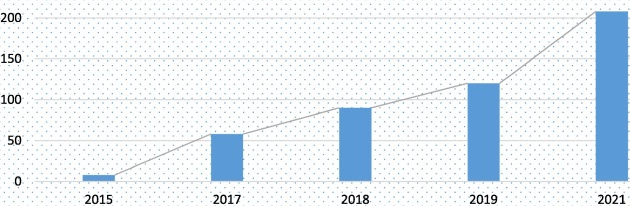
\includegraphics{images/grafica11.png}}}
\end{center}
\caption{Predicción del coste del ransomware en billones de dolares}
\label{fig:im0-es}
\end{figure}

%\change{verificar que los nombres de los labels es el mismo en la versi\'on en español e ingl\'es de la intro y conclusiones } HECHO

En la Figura \ref{fig:cove-es} se observa los resultados obtenidos de un estudio de Coveware \cite{4} sobre las industrias más afectadas por los ataques ransomware en el último trimestre del año 2020. Se puede apreciar que los servicios profesionales, el sector público y sanitario son los más afectados, ya que son los más rentables para los delincuentes. Esto se debe a su necesidad de estar en constante funcionamiento y por su posesión de datos delicados, por lo que suelen pagar los rescates para que se les devuelva sus datos y el acceso a sus sistemas lo más rápido posible.

\begin{figure}[h!]
\begin{center}
{\scalebox{.19}{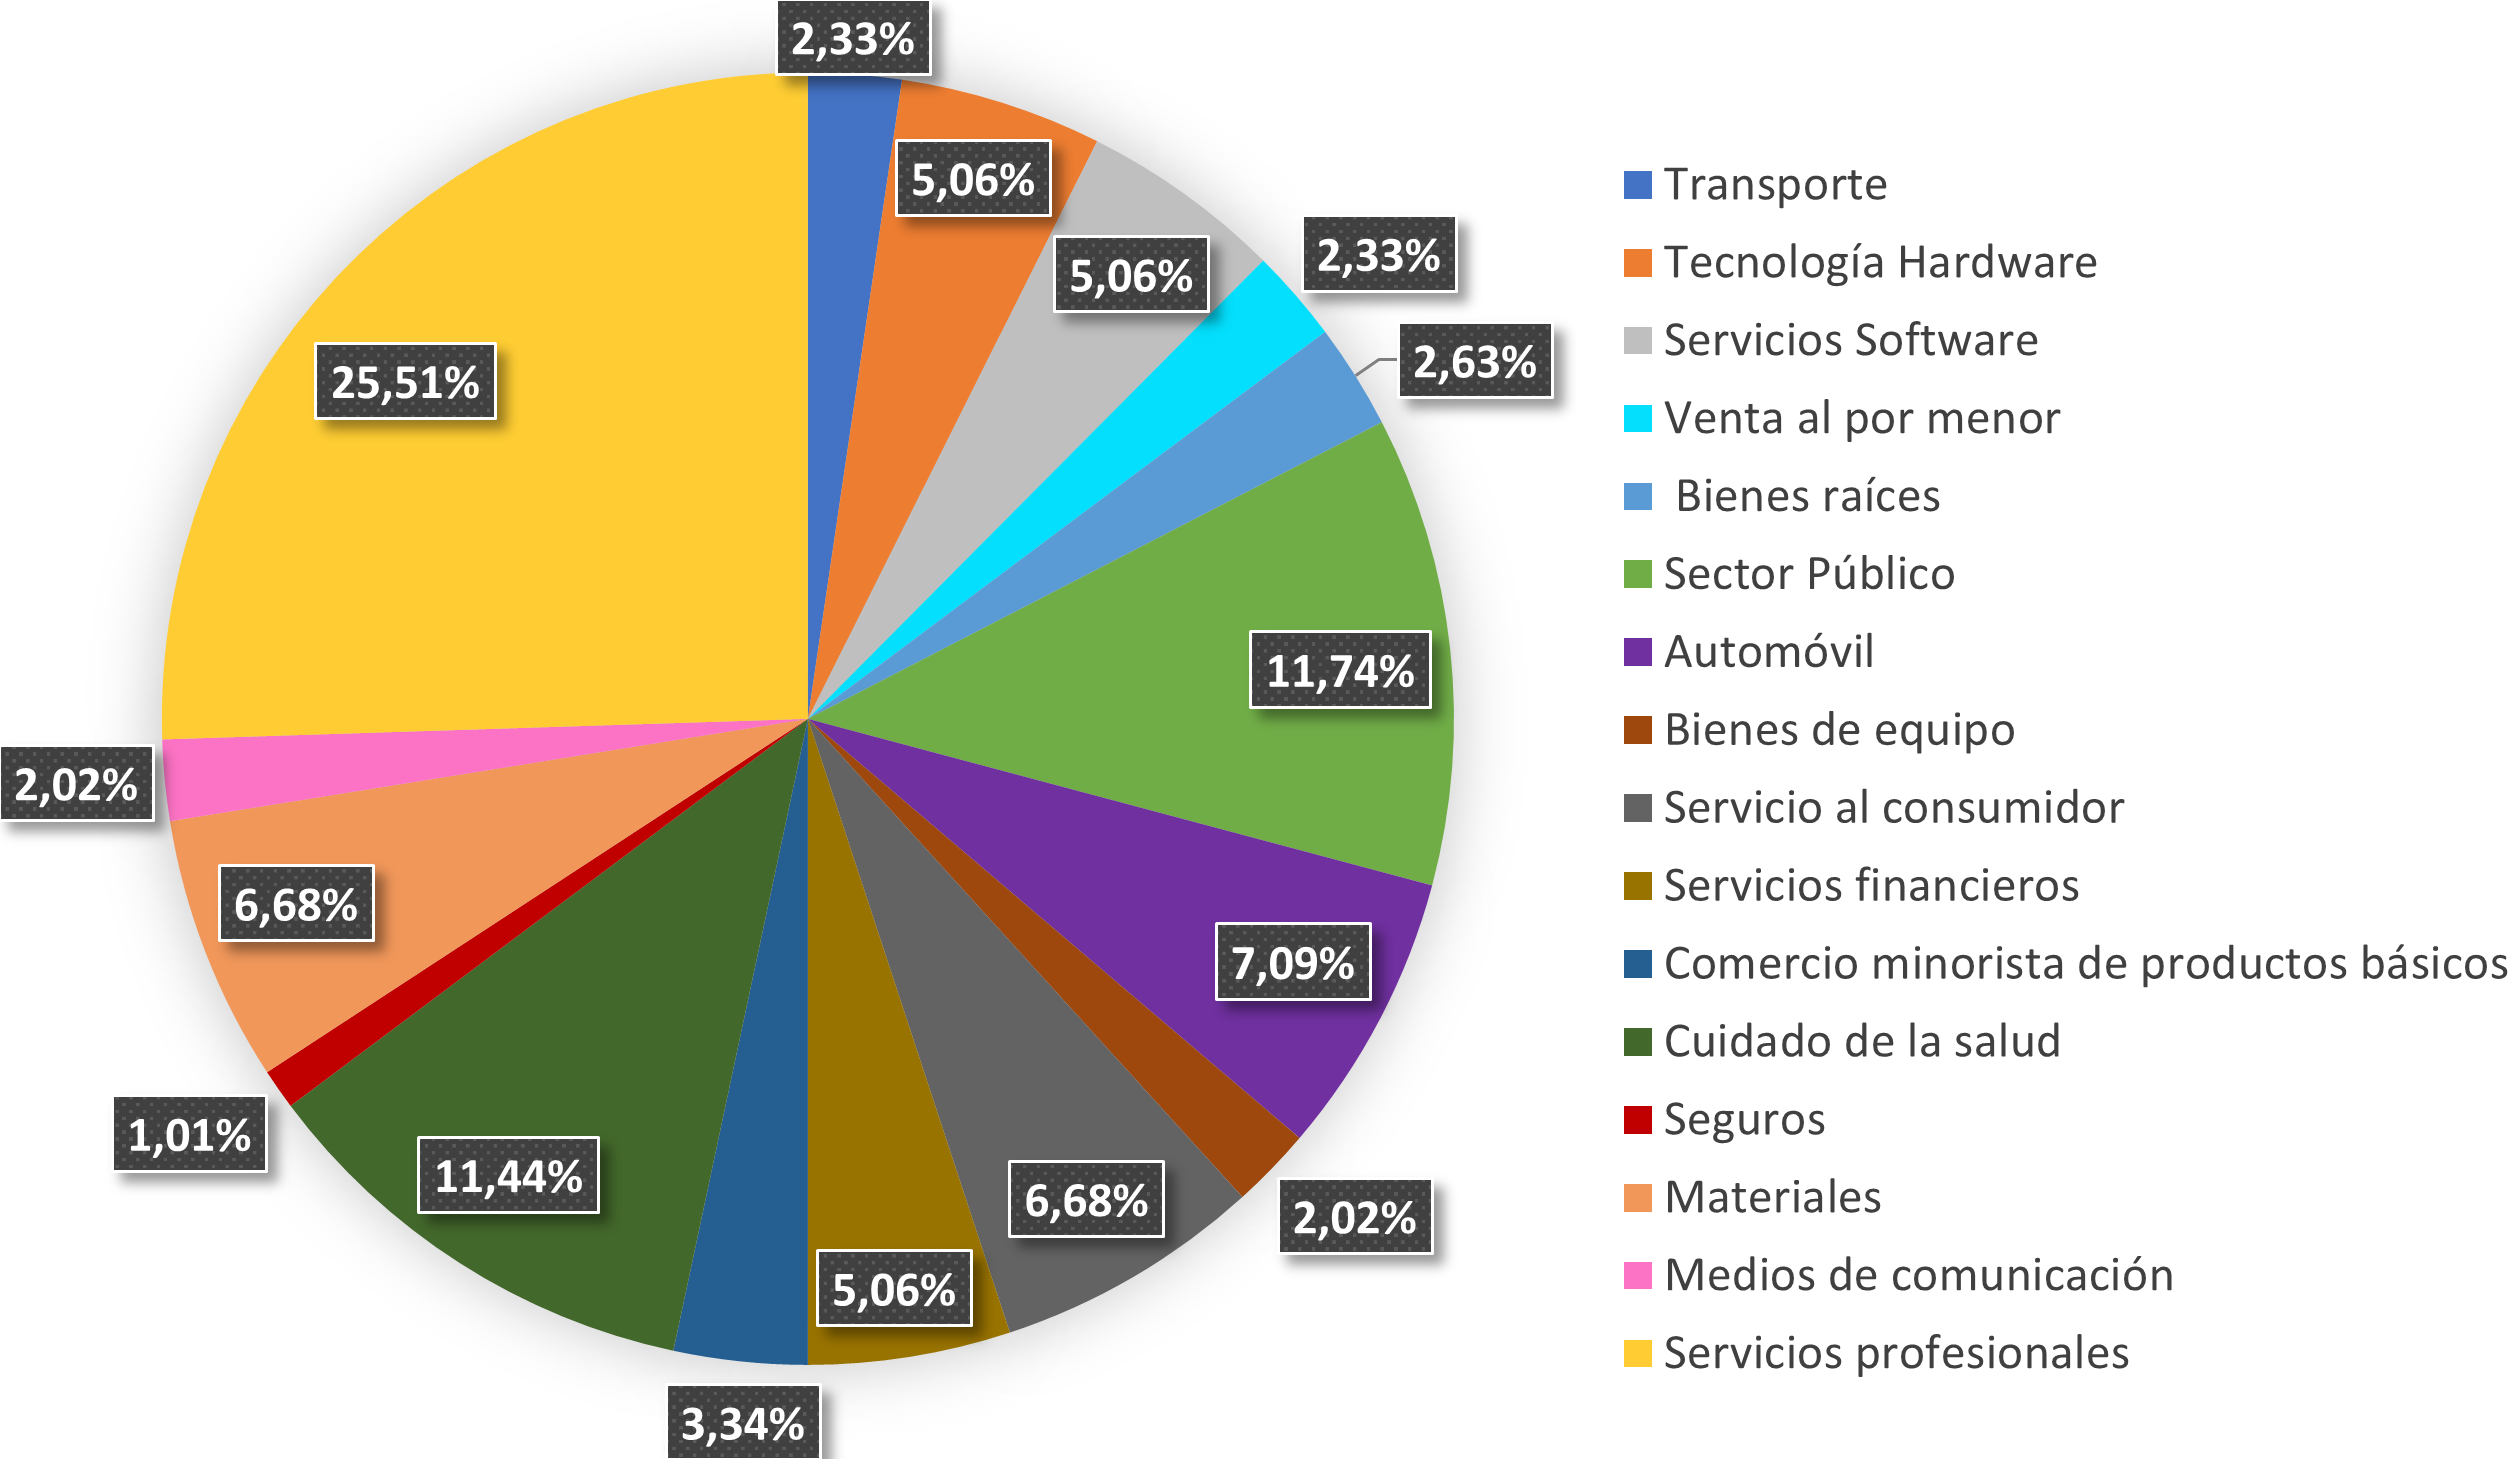
\includegraphics{images/industries2.png}}}
\end{center}
\caption{Sectores más atacados por ransomware en el tercer trimestre de 2020}
\label{fig:cove-es}
\end{figure}

El riesgo de un ciberataque es el mismo para una gran empresa que para una \gls{SME}. Estas compañías también utilizan, producen y almacenan grandes cantidades de datos. La diferencia es que las empresas más pequeñas han de lidiar con estos problemas con recursos mucho más limitados. Por lo tanto, deben hacer un mayor esfuerzo económico para trazar estrategias de seguridad ante estos ataques informáticos \cite{KURPJUHN20155}.

Al escenario planteado se le añade también la situación sanitaria actual, una la pandemia ocasionada por la enfermedad \gls{COVID-19}. Mientras esta se propagaba por el mundo, crecía una amenaza tecnológica secundaria basada en ciberataques indiscriminados y cibercampañas centradas en autoridades públicas y organizaciones \cite{LALLIE2021102248}, así como en los individuos basándose en su desinformación y temor, como la falsa distribución de libros con información sobre el \gls{COVID-19} \cite{MALWLABS}, la oferta fraudulenta de medicamentos vía correo electrónico \cite{NORTON}, etc.
Otro factor que ha favorecido el aumento de ciberataques, y en concreto, de ataques ransomware, es el establecimiento del teletrabajo. En España, estos tipos de ataques aumentaron un 160\% en el segundo semestre del año 2020, encabezando el \textit{ranking} europeo, debido a que las empresas que centraron sus esfuerzos en establecer entornos de trabajo a distancia, no aplicaron la seguridad necesaria para ello \cite{ELPAIS}. En España, las únicas empresas afectadas no han sido solo las privadas, ya que, por ejemplo, instituciones públicas recibieron ataques ransomware. El \gls{SEPE} tuvo que paralizar la totalidad de sus servicios durante 5 días, añadiendo otras 20 jornadas sin permitir el teletrabajo por un ataque en marzo de 2021 por el ransomware Ryuk, provocando una grave situación, pues la actividad del \gls{SEPE} se había disparado por el impacto de la pandemia en el desempleo \cite{RYUKSEPE}.


El desarrollo de la tecnología proporciona beneficios y facilidades en todos los ámbitos y tareas, hasta en los más cotidianos. Ejemplo de ello es el Internet de las Cosas, o \gls{IoT}, que se define como la integración de lugares y objetos de la vida real con Internet, mediante la interconexión de dispositivos, sensores, actuadores, software, etc. mediante una red, que almacena e intercambia información \cite{IoTDEF}. Sin embargo, la existencia de esta tecnología ha permitido que la cantidad de ataques ransomware crezcan con el tiempo, especialmente tras el incremento del uso de dispositivos \gls{IoT} inteligentes, particularmente los móviles. En la Figura \ref{fig:im1-es} se puede observar la cantidad de ataques ransomware a dispositivos móviles por trimestre en 2018. La Figura \ref{fig:im2-es} muestra una predicción del incremento del uso de este tipo de dispositivos debido al auge del \gls{IoT}. Con estos datos se puede predecir que la cantidad de ataques continuará en alza y se demuestra que existe una necesidad tanto de proteger a los individuos y las organizaciones de esta clase de ataques como de ofrecer la información existente a los usuarios y trabajadores  para actuar de una forma responsable y segura para prevenirlos \cite{HUMAYUN2021105}.

% IMAGEN 1
\begin{figure}[htb]
\begin{center}
{\scalebox{.4}{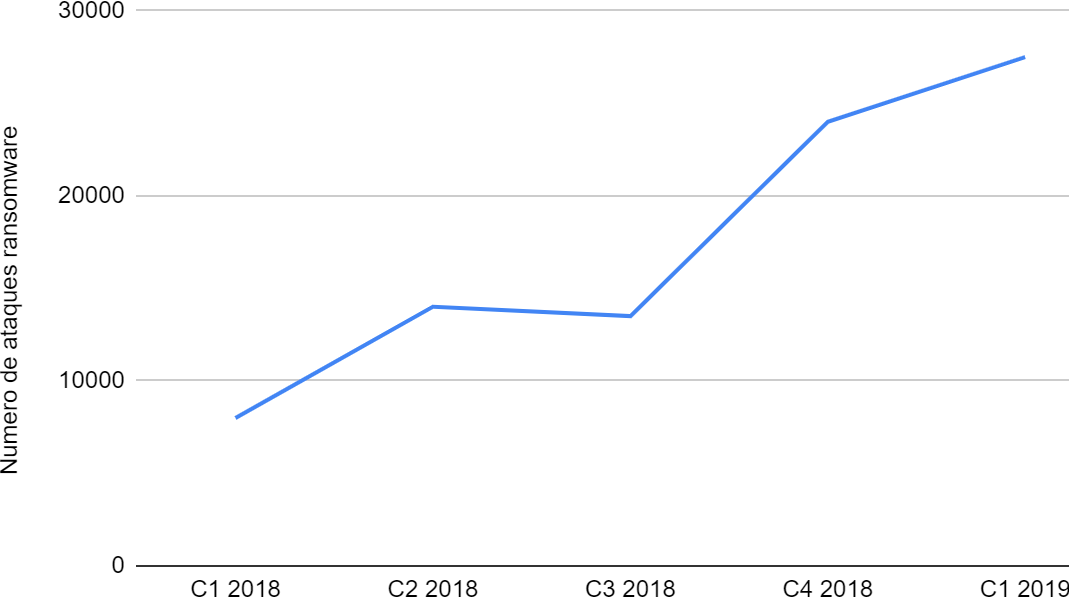
\includegraphics{images/grafica4.png}}}
\end{center}
\caption{Ataques ransomware a dispositivos móviles}
\label{fig:im1-es}
\end{figure}


% IMAGEN 2
\begin{figure}[htb]
\begin{center}
{\scalebox{.6}{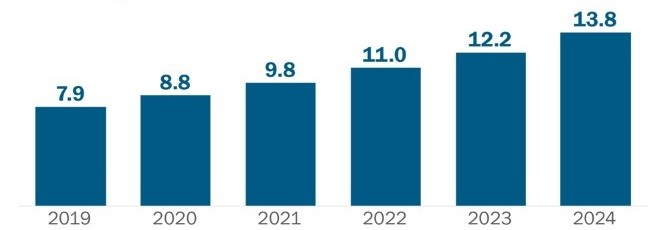
\includegraphics{images/grafica31.jpg}}}
\end{center}
\caption{Predicción de la cantidad de dispositivos IoT móviles en miles de millones}
\label{fig:im2-es}
\end{figure}


\section{Motivación}
\noindent Como se ha visto en la Sección \ref{intro}, es evidente el impacto de los ataques ransomware en las empresas en los últimos años, provocando grandes inversiones económicas para mejorar la seguridad.
Las \gls{SME} tienen mayor dificultad para afrontar dichos gastos y por lo tanto están más expuestas, debido a que no tienen sistemas de prevención, especialistas enfocados en la ciberseguridad e incluso información relativa a este sector.

En la Unión Europea, las \gls{SME} constituyen un pilar fundamental de la economía, representando en septiembre de 2020 un sorprendente 99,8\% de todas las empresas empleadoras, el 65\% del empleo del sector privado y el 54\% del sector privado de producción bruta. 
Éstas han sido además muy vulnerables a la pandemia ocasionada por el \gls{COVID-19}, provocando grandes pérdidas e incluso gran cantidad de cierres \cite{NBER}. 
Debido a todos estos factores, la motivación principal de este estudio es el desarrollo de un modelo de detección de ransomware que cumpla con los siguientes requisitos: Precisión, fiabilidad, escalabilidad, facilidad de uso, rapidez y software libre.

De esta manera se puede llevar a cabo una estrategia de prevención contra ataques ransomware y reducir el impacto de los daños ocasionados por ellos a través de una herramienta accesible a las \gls{SME}, reduciendo de manera drástica los costes de inversión.


%\section{Contexto}
%\noindent Este Trabajo Fin de Grado ha sido realizado dentro del Grupo de Análisis, Seguridad y Sistemas (Grupo GASS \cite{GASS01}, \url{https://gass.ucm.es/}, Grupo 910623 del catálogo de grupos reconocidos por la \gls{UCM}) como parte de un proyecto de investigación aprobado por la Comisión Europea. %decir que nos digan detalles de esto


\section{Objetivos}
\noindent Al inicio del trabajo, se establecen una serie de objetivos para asegurar su calidad y fijar unas pautas para el correcto desarrollo:
\begin{itemize}
    \item Utilizar las competencias adquiridas durante el grado.
    \item Desarrollar un modelo de \gls{ML} capaz de identificar muestras de ransomware con gran precisión.
    \item Construir un extenso \textit{dataset} para garantizar la fiabilidad en los resultados obtenidos. 
    \item Desarrollar y desplegar un laboratorio para el análisis de muestras de malware.
    \item Demostrar la efectividad de las llamadas a las \gls{API} de Windows de un ejecutable como mecanismo de detección de ransomware. %Comprobar, a su vez, la mejora del comportamiento al utilizar la cantidad de llamadas en lugar de su aparición única. %yo esto lo quitaria
\end{itemize}


\section{Plan de Trabajo}
\noindent El desarrollo de este trabajo se ha realizado en las siguientes fases:
\begin{enumerate}
    \item \textbf{Investigación}: Esta fase se llevó a cabo durante los primeros cuatro meses, donde se adquirió la información necesaria para el desarrollo del trabajo. Al comienzo de la fase, se realizaron varias reuniones donde se explicaron los objetivos del proyecto y los conocimientos necesarios, siendo estos los conceptos fundamentales del aprendizaje automático. Una herramienta primordial para la investigación fue \textit{Google Scholar}, ya que permite buscar artículos científicos y citarlos con facilidad. Se buscaron artículos y publicaciones sobre detección tanto de ransomware como de malware, además de libros sobre análisis malware para adquirir conocimientos más profundos del tema y entender el contexto del trabajo.
    \item \textbf{Desarrollo}: Una vez obtenidos los conocimientos necesarios, se comenzó el desarrollo del modelo. No se abandonó por completo la investigación, pero pasó a un segundo plano. Durante esta fase se obtuvieron los datos necesarios y se construyeron los dos \textit{datasets} para entrenar y evaluar el modelo propuesto. Posteriormente se pasó a la familiarización con el lenguaje de programación Python y con la librería \textit{scikit-learn}, usada para la codificación del modelo y la implementación de los algoritmos de \gls{ML}.
    \item \textbf{Experimentación y resultados}: En esta fase experimentó con el modelo desarrollado y los datos extraídos. Al obtener los resultados era necesario evaluarlos y demostrar la validez del modelo, por lo que se usó la validación cruzada K-Fold. La experimentación fue vital para la fase de desarrollo, ya que se tuvo que modificar el modelo para mejorar los resultados, ajustando los parámetros, obteniendo más datos...
    \item \textbf{Documentación}: La fase de documentación se llevó a cabo de manera paralela al resto de fases. Empezó en los últimos meses de la fase de investigación con los conocimientos asentados, y continuó durante el desarrollo y la experimentación. Todos los miembros del equipo participaron en la escritura de la memoria, trabajando en conjunto en todas las secciones. Cualquier actualización debía de ser aceptada y revisada por los otros miembros del equipo.
\end{enumerate}

El modelo desarrollado en este trabajo está subido en el repositorio de Gitlab \href{https://gitlab.fdi.ucm.es/marina.lopez/tfg-ransomware-20-21}{TFG Ransomware 20-21}.


%\change{Agregar las actividades realizadas en y el diagrama de Gannt}
La Figura \ref{fig:gantt} es un diagrama de Gantt donde se pueden apreciar las actividades desempeñadas por el equipo a lo largo de los meses y su duración.

\begin{figure}[htb]
\begin{center}
{\scalebox{.9}{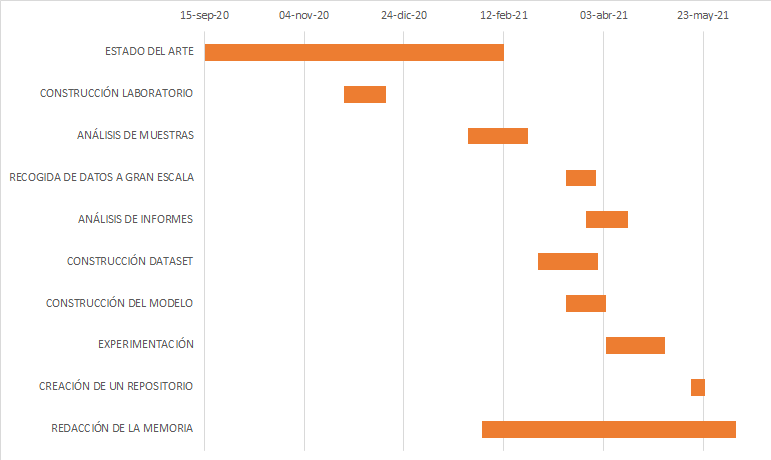
\includegraphics{images/gant.png}}}
\end{center}
\caption{Diagrama de Gantt de las tareas desempeñadas.}
\label{fig:gantt}
\end{figure}

\section{Estructura del Trabajo}
\noindent El resto del trabajo está organizado en 10 capítulos, siguiendo esta estructura:

%\Ransomware
El Capítulo \ref{Capitulo2} introduce el ransomware, explicando los conceptos fundamentales sobre el malware y los diferentes tipos, el modelo de negocio que siguen los ciberdelincuentes para sacar beneficio de los ataques y la evolución histórica del ransomware, detallando cada año los diferentes ataques que han habido en el mundo. También se exponen los diferentes tipos de ransomware, las familias, los métodos de propagación más comunes y posteriormente el modo de operación para infectar el sistema de la víctima. El capítulo termina explicando algunas técnicas usadas por programas antivirus para reconocer la presencia del ransomware y unas estrategias y acciones de prevención que toda empresa debería seguir para proteger sus sistemas de estos ataques, y en caso de sufrirlos, que pasos deberían seguir para recuperas sus datos.

%Análisis e identificación de malware
El Capítulo \ref{Capitulo3} aborda los tipos de análisis de malware que existen, las herramientas que se usan, las limitaciones de cada uno y las diferentes técnicas de identificación. Posteriormente se habla del aprendizaje automático aplicado al análisis malware, exponiendo cómo se construye un modelo de \gls{ML} usando Python como lenguaje de programación y los diferentes algoritmos que existen, indagando en los denominados algoritmos de aprendizaje supervisado, ya que son los que más se utilizan en análisis y detección de malware y ransomware.

%Estado del arte
El Capítulo \ref{Capitulo4} se muestran trabajos relacionados con el tema de análisis y detección de malware y ransomware usando modelos de \gls{ML} y algoritmos de aprendizaje automático. Se distinguen entre trabajos que solo analizan malware de los que analizan ransomware, y dentro de los trabajos de ransomware se diferencian los que usan las llamadas a la \gls{API} de Windows para construir sus modelos de los que no.

%Arquitectura y tecnologías utilizadas (Sistema Propuesto)
El Capítulo \ref{Capitulo5} expone las tecnologías usadas para desarrollar el modelo de \gls{ML}, el entorno de trabajo y la obtención de los datos. Se muestra el diagrama de flujo del sistema propuesto y se habla sobre el desarrollo del laboratorio de análisis para el estudio de las muestras de ransomware y goodware, de las cuales se extraen las llamadas a la \gls{API} de Windows para la construcción de los \textit{datasets}. Posteriormente se hace una limpieza de los datos en los \textit{datasets} para descartar aquellos que no son relevantes para el estudio y se explica cómo se creará el modelo.

%Experimentos y resultados
El Capítulo \ref{Capitulo6} aborda los experimentos realizados y las métricas utilizadas para demostrar la efectividad del modelo para detectar ransomware. Después de mostrar los experimentos sobre los dos \textit{datasets} y los parámetros utilizados para su desarrollo, se obtienen los resultados finales y se validan con la validación cruzada K-fold. Posteriormente se elige el algoritmo que mejores resultados ha obtenido y se comparan con los resultados de los trabajos relacionados expuestos en el Capítulo \ref{Capitulo4}.

%Conclusiones y trabajo futuro
El Capítulo \ref{Capitulo7} muestra las conclusiones del trabajo tras el análisis de los resultados y expone las líneas de investigación futuras.

%Contribucion de cada uno
El Capítulo \ref{Capitulo8} relata las aportaciones individuales de cada miembro del equipo al desarrollo del trabajo.

%Ingles
Los Capítulos \ref{Capitulo9} y \ref{Capitulo10} son las traducciones al inglés de los Capítulos \ref{Capitulo1} y \ref{Capitulo7}. 
	
\chapter{Ransomware}\label{Capitulo2}
%\change{Todos los capítulos deben empezar con un p\'arrafo de este estilo. Usar verbos en presente en tercera (ej. realiza, describe, etc.).}
%\change{Colocar la primera letra en may\'uscula cuando se usa el comando ref. Por ejemplo Figura XX, Cap\'itulo XX, Secci\'on XX, Tabla XX. - HECHO}%solucionado en todos los capitulos
%\change{Como el siguiente p\'arrafo:\\
%cifrar en vez
%de encriptar\\
%" o “ cambiarlas por ``(apertura) y '' (cierre)}%solucionado
%\change{algunas figuras est\'an muy grandes, rediseñarlas para optimizar el espacio. Que sean m\'as anchas que largas, para que se aproveche el ancho de la p\'agina}
%\change{Todos los títulos de secciones y cap\'itulos debe ir la primera letra de cada palabra en mayúsculas salvo art\'iculos y preposiciones-HECHO}%solucionado en todos los capitulos
%\change{Graficas con titulo en new roman}


%MAL
%\st{En este cap\'itulo  se profundiza en lo que concierne a este estudio, el ransomware, uno de los tipos de malware con m\'as impacto en la actualidad, su evolución hist\'orica, las diferencias con respecto otros tipos de malware, las familias más importantes, las t\'ecnicas de prevenci\'on y una secci\'on una sección que explica c\'omo lidiar con un equipo infectado por ransomware. Pero para contextualizar, primero se considera necesario exponer conceptos fundamentales sobre el malware, sus tipos y su modelo de negocio.  }

\noindent En este capítulo se realiza un estudio detallado sobre ransomware. Los conceptos fundamentales sobre el malware, sus tipos y su modelo de negocio se presentan en la Sección \ref{sec:2-1}. Los tipos de malware con mayor impacto en la actualidad. En la Sección \ref{sec:2-2} se define el ransomware y se enumeran las principales diferencias con respecto otros tipos de malware. Su evolución histórica, los tipos  y las familias más importantes se detallan en la Secciones \ref{sec:2-3} a \ref{sec:2-5}. En la Sección \ref{sec:2-6} se exponen los diferentes vectores de ataque y los métodos de operación analizan en la Sección \ref{sec:2-7}.  Las técnicas de detección y prevención de los ataques de ransomware así como las recomendaciones para el post-ataque se explican en las Secciones \ref{sec:2-8} a \ref{sec:2-10}.

\section{Malware}\label{sec:2-1}
\noindent Malware es una abreviación de software malicioso. Se trata de programas o fragmentos de código que ganan acceso o provocan daño en un ordenador, sin necesidad de que su propietario lo sepa. El malware utiliza canales de comunicación populares como el correo electrónico o descargas desde páginas web para expandirse. Su finalidad es explotar vulnerabilidades del sistema. Este software ajeno se instala en el equipo y realiza tareas no deseadas, como la aparición de continua y molesta publicidad en la pantalla, pero incluso puede ser utilizado para obtener beneficios económicos a terceros, mediante el robo de información o infección de redes \cite{mwdef}. El malware se clasifica dependiendo de su modo de operación, que pueden ser los siguientes \cite{virusbomb}:
\begin{enumerate}
    \item \textbf{Auto-replicación}: Intenta propagarse mediante las copias o instancias de él mismo. De modo análogo, otros tipos de malware se copian de manera pasiva, por error de algún usuario, por ejemplo.
    \item \textbf{Expansión de la infección}: Describe la capacidad de crecimiento en el número de instancias creadas. Aquellos que se reproducen mediante auto-replicación crecen de manera mucho más rápida. 
    \item \textbf{Parasitario}: Requiere otro código ejecutable para existir.
\end{enumerate}

\subsection{Tipos de Malware}
\noindent Los tipos de malware más importantes son:

\begin{itemize}
    \item \textbf{Virus}: Un virus es un tipo de malware parasitario y con crecimiento exponencial que, cuando se ejecuta, intenta replicarse en otro código ejecutable. Cuando lo consigue, se dice que dicho código ha sido infectado. El código infectado, cuando se ejecuta, puede a su vez infectar nuevo código. Este modo de auto-replicarse en código existente en un computador es la característica definitoria de un virus. Tradicionalmente, los virus se pueden propagar en un solo ordenador, o migrar de unos a otros, transportados a través de un humano, vía \gls{USB}, \gls{CD-ROM} o \gls{DVD}, pero nunca a través de ninguna red \cite{virusbomb}.
    
    \item \textbf{Spyware}: Una clase de código malicioso que se instala de manera encubierta en la máquina de la víctima, y una vez activo, silenciosamente monitoriza el comportamiento de los usuarios, graba sus hábitos al navegar en la red y sustrae sus archivos sensibles y contraseñas. También permite realizar capturas de pantalla, obtener información de la cámara y el micrófono, evitar ser desinstalado e incluso instalar software \cite{articleSpy}.  Normalmente, la información recogida es enviada al distribuidor de \textit{spyware}, y posteriormente utilizada para realizar estudios de publicidad o marketing, e incluso vendida a terceros. Una de las técnicas más importantes es explotar las vulnerabilidades de los navegadores \cite{Egele2007DynamicSA}.
    
    \item \textbf{Adware}: Es considerada una forma menos dañina de \textit{spyware}. Mientras que el \textit{spyware} trabaja de manera encubierta, el \textit{adware} es evidente. Algunas de sus formas de actuar pueden ser cambiar la página de inicio de un navegador, modificar el contenido de páginas web para insertar anuncios, realizar un seguimiento del comportamiento del usuario y transmitir dicha información, que puede ser manteniendo o no la privacidad del usuario, para obtener algún beneficio \cite{articleSpy}.
    
    \item \textbf{Trojans}: Denominados así en referencia al caballo de madera utilizado por los griegos en el asedio a Troya, debido a que el código malicioso entra en el equipo camuflado, normalmente mediante algún archivo descargado al abrir un correo electrónico extraño. Este tipo de malware parasitario permite a su creador ejecutar comandos sin autorización en un equipo infectado. Permite a los \textit{hackers} modificar ajustes de los archivos, robar información o contraseñas, realizar daños en el equipo, apagarlo o incluso
    deshabilitar antivirus u otros mecanismos de seguridad. Actúan según la Figura \ref{fig:imtroyano} \cite{trojan}.
    
     \begin{figure}[htb!]
        \begin{center}
        \subfigure[Fase I]{
            {\scalebox{.6}{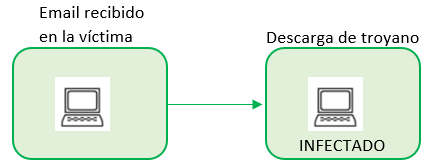
\includegraphics{images/troyano1.png}}}
            \label{fig:troj1}}
        \subfigure[Fase II]{
            {\scalebox{.6}{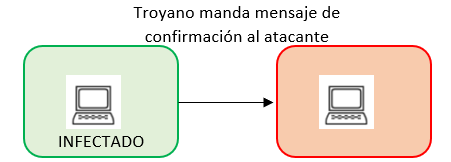
\includegraphics{images/troyano2.png}}}
            \label{fig:troj2}}
        \subfigure[Fase III]{
            {\scalebox{.6}{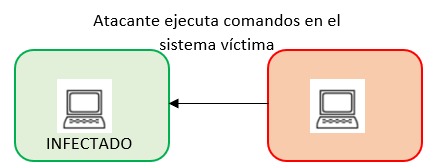
\includegraphics{images/troyano3.png}}}
            \label{fig:troj3}}
        \caption{Flujo de acción de un troyano}
        \label{fig:imtroyano}
        \end{center}
        \end{figure}
    
    
    
    \item \textbf{Worms}: Es un código malicioso que se origina en un único ordenador y busca otros equipos conectados a un área local \gls{LAN} o mediante una conexión a Internet. Cuando el gusano encuentra otro ordenador, se replica en dicho equipo y continúa buscando más ordenadores. Un gusano sigue intentando replicarse indefinidamente o hasta que expira un temporizador, tal como muestra la Figura \ref{fig:im4} \cite{trojan}.
    %\change{Usar la primera letra en mayúscula Figura XX, la Tabla XX. La figura 2.1 no está clara}
    
    \begin{figure}[htb]
    \begin{center}
    {\scalebox{.8}{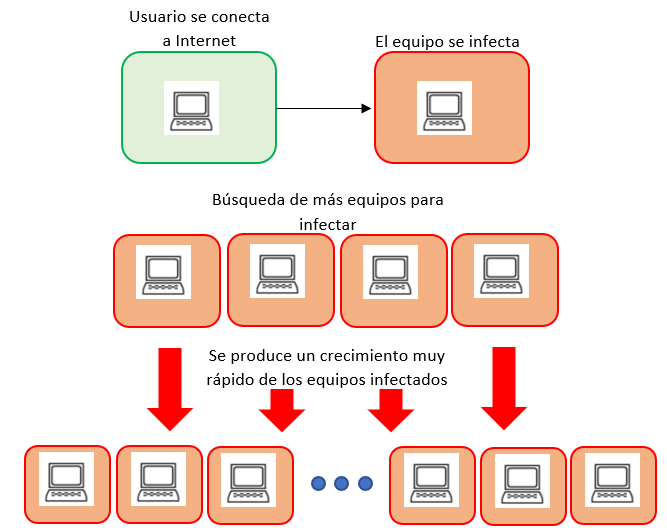
\includegraphics{images/gusano.png}}}
    \end{center}
    \caption{Infección de equipos por gusano}
    \label{fig:im4}
    \end{figure}
    
    \item \textbf{Logic Bomb}. Código malicioso que consiste en una ``carga explosiva'', que puede ser cualquier acción maligna para el equipo víctima, y un disparador: una condición booleana que controla cuando se va a ejecutar la ``carga explosiva'' \cite{virusbomb}.
    %\change{" o “ cambiarlas por ``(apertura) y '' (cierre)}
    
    \begin{algorithm}[htb!]
\renewcommand{\lstlistingname}{Algoritmo}
\begin{lstlisting}[language=config, caption={Ejemplo de bomba lógica sencilla}, captionpos=b, firstnumber=1, linewidth=14.4cm]
    //Codigo legitimo
    if fecha is Viernes 13 then
        apagar_ordenador()
    //Codigo legitimo
    \end{lstlisting}
\label{Alg:imx1}
\end{algorithm}
%\change{utilizar esta forma de hacer los algoritmos o trozos de c\'odigos. Referenciar los algoritmos así como las figuras}

        
\end{itemize}
\subsection{Ingeniería Social Aplicada al Malware}
\noindent La ingeniería social consiste en una serie de técnicas psicológicas y habilidades sociales que permiten persuadir a las personas para obtener de ellas información, ya sea personal o profesional, o para conseguir acceso a su sistema o red. Se basa en una metodología que sigue estas fases \cite{GallegosSegovia2017}:
\begin{enumerate}
    \item \textbf{Recogida de información}: En esta fase se obtiene información sobre la víctima para establecer posibles vectores de ataque.
    \item \textbf{Obtención de confianza}: Las personas tienden a revelar información o secretos con aquellos en quien confían. Debido a esto, el atacante trata de obtener una relación de confianza con la víctima.
    \item \textbf{Fase de aprovechamiento}: La relación de confianza establecida da lugar a la petición de información o la acción requerida. 
    \item \textbf{Fase final}: Los resultados obtenidos en la fase anterior son usados para realizar el ataque planeado previamente.
\end{enumerate}
Los tipos fundamentales de ingeniería social utilizados para realizar ataques malware son los siguientes \cite{GallegosSegovia2017}:
\begin{itemize}
    \item \textbf{Ataques técnicos}: No existe interacción física con la víctima. Se usan herramientas como el correo electrónico o las descargas en la web. Su principal amenaza es que intentan parecer entidades reconocidas y fiables, utilizando logos comerciales, platillas de mensajes, etc.
    \item \textbf{Ataques de ego}: Existe un contacto directo entre el atacante y la víctima.  Los criminales ofrecen ayuda demostrando su inteligencia, de forma que las víctimas caen en un tipo de manipulación transparente, y proporcionan la información con facilidad. 
    \item \textbf{Ataques de simpatía}: Se crea una relación de confianza con la víctima, la cual siente empatía por el atacante. Se basa en el uso de técnicas conversacionales para generar una comunicación espontánea, de manera que la víctima se siente segura y expone sus vulnerabilidades.
    \item \textbf{Ataques de acoso}: Se basan en la intimidación, amenazas y coacción para obtener información.
\end{itemize}

\section{Definición de Ransomware}\label{sec:2-2}
\noindent Ransomware, o secuestro de datos, es un tipo de malware, con características típicas de malware, pero a su vez con sus propias peculiaridades. Se basa en la inyección de procesos en programas destino, que provocan la extracción de datos del usuario y permite la comunicación segura con el servidor de mando y control \gls{CyC}. Su principal objetivo es cifrar los archivos privados del sistema víctima o inutilizar el equipo y forzar al pago por su rescate. El código ransomware es relativamente fácil de encontrar por la web, escribir y modificar. Esta simplicidad del código combinada con su naturaleza lucrativa, ha resultado en la generación explosiva de gran cantidad de variantes \cite{DEFRANSW}. 
El ransomware se diferencia de otros tipos de malware por las siguientes características \cite{ransommasive}:

\begin{itemize}
    \item La finalidad del ransomware es extorsionar dinero a las víctimas, sin dañar el sistema operativo o los datos de manera irreversible, mientras que otros tipos de malware únicamente buscan convertir en inoperante el equipo.
    
    \item No requiere privilegios de administrador para cifrar los archivos.
    
    \item La habilidad tanto de cifrar archivos como de modificar su nombre, hace inconsciente a la víctima de la cantidad de archivos cifrados.
    
    \item Utilizan diferentes métodos para evadir mecanismos de seguridad como \textit{firewalls} o antivirus.
    
    \item Algunos tipos conectan el equipo víctima a \textit{botnets} para otros ciberataques posteriores.
    
    \item Los ataques son independientes de la localización geográfica y del lenguaje del área.
    
\end{itemize}

\section{Historia del Ransomware}\label{sec:2-3}

\noindent El ransomware ha sido una amenaza importante para todo tipo de empresas desde mediados de la década del 2000, pero eso no significa que no haya habido ataques anteriores. Su historia se puede estructurar en dos fases según el tipo de acciones malignas que el malware realiza en el equipo \cite{histRansom}:
\begin{enumerate}
    \item \textbf{Bloqueo de equipo}: En esta etapa se restringía el acceso al sistema operativo, obligando a la víctima a pagar un rescate para poder utilizar su equipo. Este tipo de ataques comenzó a acarrear gran riesgo por parte de los atacantes debido a que los expertos informáticos aprendieron a luchar contra ellos atacando directamente a los pagos electrónicos.
    \item \textbf{Cifrado de información}: Con el nacimiento de las cripto-monedas y habiendo eliminado a los intermediarios en los pagos, como los bancos y al ser imposible su rastreo, surge este tipo de ataque, por el cual se pide un rescate a usuarios y empresas tras cifrar archivos con claves robustas, ofreciéndoles mayor cantidad de beneficios de una manera más segura para los atacantes.
    
\end{enumerate}

El primer ransomware conocido fue el AIDS Trojan, también llamado PC Cyborg Trojan. Fue creado en 1989 por Joseph Popp, un biólogo estadounidense, y distribuido a través de disquetes en una conferencia de la OMS y enviados a través de los servicios postales. Estos disquetes venían en sobres con el remitente ``PC Cybor Corporation'' y decían tener información sobre el SIDA, por lo que fueron enviados a investigadores alrededor del mundo. Se distribuyeron alrededor de 20.000 disquetes en más de 90 países. Usaba criptografía simétrica simple para cifrar nombres de archivos del sistema y hacía que las impresoras conectadas imprimieran una nota de rescate pidiendo al usuario enviar \$189 dólares a un buzón en Panamá para que pudieran recibir el software que desbloquearía su ordenador. Este ransomware causó daños severos al campo científico, haciendo que compañías perdieran todo su trabajo de investigación sobre el tratamiento del SIDA \cite{51}, y fue la base para la evolución del ransomware hacia los ataques más sofisticados que se llevan a cabo hoy en día. %Los primeros desarrolladores de ransomware normalmente escribían su propio código de cifrado, pero hoy en día los atacantes dependen cada vez más del \gls{RaaS}, lo que ha llevado al aumento substancial de los ataques. También se aprovechan de métodos de entrega más sofisticados, como campañas de \textit{spear-phishing}, que es un tipo de \textit{phising} más efectivo por estar dirigido a una organización en específico, siendo una estafa más elaborada \cite{53}.


El siguiente gran paso en la evolución del ransomware fue en 1996, cuando dos investigadores presentaron un artículo en la Conferencia de Seguridad y Privacidad de IEEE llamado \textit{Cryptovirology: extortion-based security threats and countermeasures} \cite{54}. Este documento expuso un programa que usaba cifrado de la clave pública para crear código malicioso que afectara al ordenador infectado y extorsionara a las víctimas para que pagaran una cuantía de dinero por el rescate de su sistema. El documento sugirió los términos \textit{cryptoviral extortion} y \textit{cryptovirology} para nombrar este tipo de ciberataque, que es lo que hoy en día se conoce como ransomware \cite{8}.


Antes del 2005 el ransomware no era muy popular entre los delincuentes y no se produjeron ataques importantes. Sin embargo, esto cambió drásticamente en 2005, cuando los desarrolladores de malware comenzaron a utilizar el cifrado en su código malicioso, creando ransomware de tipo Filecoder. Conocido como el primer ransomware moderno, Trojan Gpcoder o GP Code, fue el más notable ya que utilizaba cifrado \gls{RSA} de 1024 bits, un cifrado fuerte en ese momento, lo que dificultaba la recuperación de los archivos afectados y se propagaba adjunto a correos electrónicos, simulando ser una aplicación de trabajo. Después de GPCoder, surgieron otras familias como Krotten y Cryzip \cite{40}.


En 2007 apareció el primer ransomware de tipo Lockscreen llamado WinLock. Este ransomware se hacía con el control de la pantalla de la víctima y mostraba imágenes inapropiadas junto con un mensaje. Este mensaje informaba al usuario que tenía que pagar un rescate a través de \gls{SMS} para desbloquear su sistema \cite{56}.


En 2009 surgió el primer ataque de un ransomware de tipo Scareware llamado Vundo, y esto supuso el salto a la monetización intensiva de este tipo de crímenes, ayudados por la proliferación de plataformas anónimas de pago en línea. Los delincuentes comprendieron que se podía ganar dinero con el ransomware y este hecho fue el detonante del rápido crecimiento del número de amenazas cada vez más complejas. En 2011, estos tipos de ransomware estaban en auge, detectándose 60.000 nuevos ataques, y en 2012, esa cifra había aumentado hasta los 200.000. Se estimó que, a finales del 2012, el mercado negro de ransomware tenía un valor aproximado de \$5 millones. El ransomware más notable que utilizó tales tácticas para hacerse pasar por agencias de la ley fueron Reveton y Kovter. Reveton cobró los rescates utilizando \textit{bitcoins} y tarjetas anónimas de pago como \textit{MoneyPak} \cite{55}.

%Impulsados por el éxito de Reveton, diferentes variantes de ransomware comenzaron a aparecer entre 2013 y 2015.

CryptoLocker apareció en 2013 y usaba criptografía de clave pública y privada (\gls{AES} y \gls{RSA} de 2048 bits) para cifrar y descifrar los archivos de las víctimas. Fue distribuido por un correo electrónico que simulaba proceder de UPS o FedEx y la versión original de CryptoLocker cifraba alrededor de 67 tipos diferentes de archivos y daba a las víctimas 3 días para pagar. El precio del rescate rondaba entorno a 2 \textit{bitcoins} o 100 dólares. En diciembre de aquel año, se descubrió que 250.000 máquinas fueron infectadas y en torno a 42000 \textit{bitcoins} de rescate habían sido pagados.
Esto provocó un crecimiento explosivo en los pagos de rescate, que alcanzaron más de \$325 millones a finales de 2015 \cite{8}. CryptoLocker fue el primer caso de propagación de ransomware a través páginas web infectadas mediante de la \textit{botnet} llamada Gameover Zeus. No obstante, CryptoLocker también se difundía mediante \textit{spear-phishing} o en correos electrónicos no deseados como un archivo adjunto \cite{55}. La desaparición de CryptoLocker por el cierre de sus servidores \cite{cryptoLock}, condujo a la aparición de varias imitaciones como CryptoWall y TorrentLocker. 

En 2015, CryptoWall superó a CryptoLocker como la versión líder de ransomware, que aprovechaba una vulnerabilidad de Java y se distribuía a través de anuncios maliciosos. En este mismo año aparecieron \gls{RaaS}, un modelo por el que los atacantes distribuían su ransomware mediante la web \gls{TOR}, repartiéndose los beneficios entre los autores y los grupos que realizaban el ataque. CryptoWall fue una de las familias más utilizadas entre abril de 2014 y principios de 2016, habiendo ganado más de \$18 millones \cite{52}. En la Figura \ref{fig:imkap}, realizada con los datos de un estudio de Kaspersky \cite{40}, se puede ver la distribución de todas las variantes de ransomware que surgieron entre los años 2014 y 2015, siendo CryptoWall el más popular después de la caída de CryptoLocker.

\newpage

\begin{figure}[h!]
\begin{center}
{\scalebox{.75}{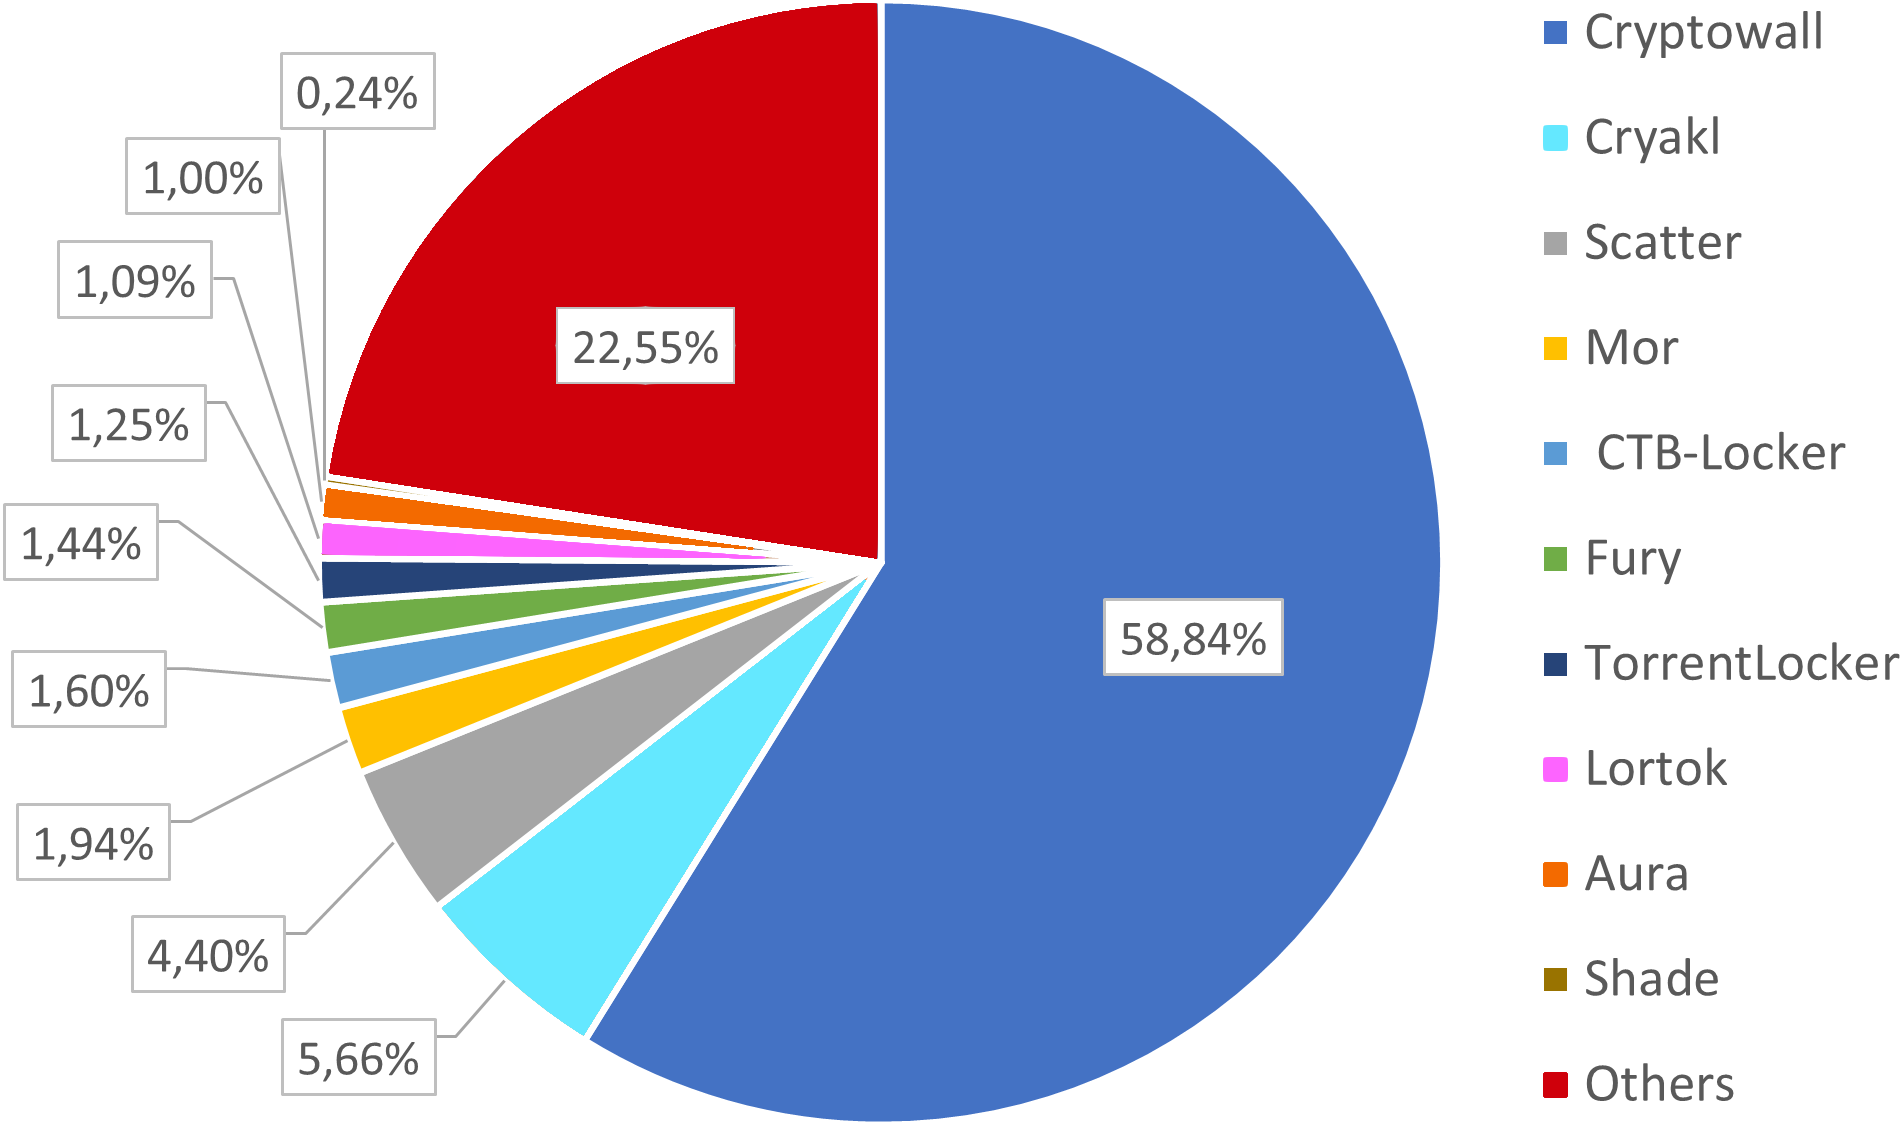
\includegraphics{images/2014-2015.png}}}
\end{center}
\caption{Familias de ransomware más observadas entre 2014 y 2015.}
\label{fig:imkap}
\end{figure}%Marina
%\change{Las gr\'aficas no deben tener el título insertado. Colocar el texto de las figuras en times new roman - HECHO}

En mayo de 2016, ZDNet publicó un artículo \cite{57} donde informaba que las tres principales familias de ransomware más usadas a principios del año fueron Teslacrypt (58,4\%), CTB-Locker (23,5\%) y Cryptowall (3,4\%). A mediados de 2016 surgió Locky y se hizo con el primer puesto, superando a CryptoWall y a Teslacrypt a principios de febrero y solo siendo adelantado por Cerber en junio. El Gráfico \ref{fig:imphish} se ha realizado con los datos de una investigación realizada por PhishMe \cite{6} que estudia todos los hechos mencionados anteriormente.

\begin{figure}[h!]
\begin{center}
{\scalebox{.72}{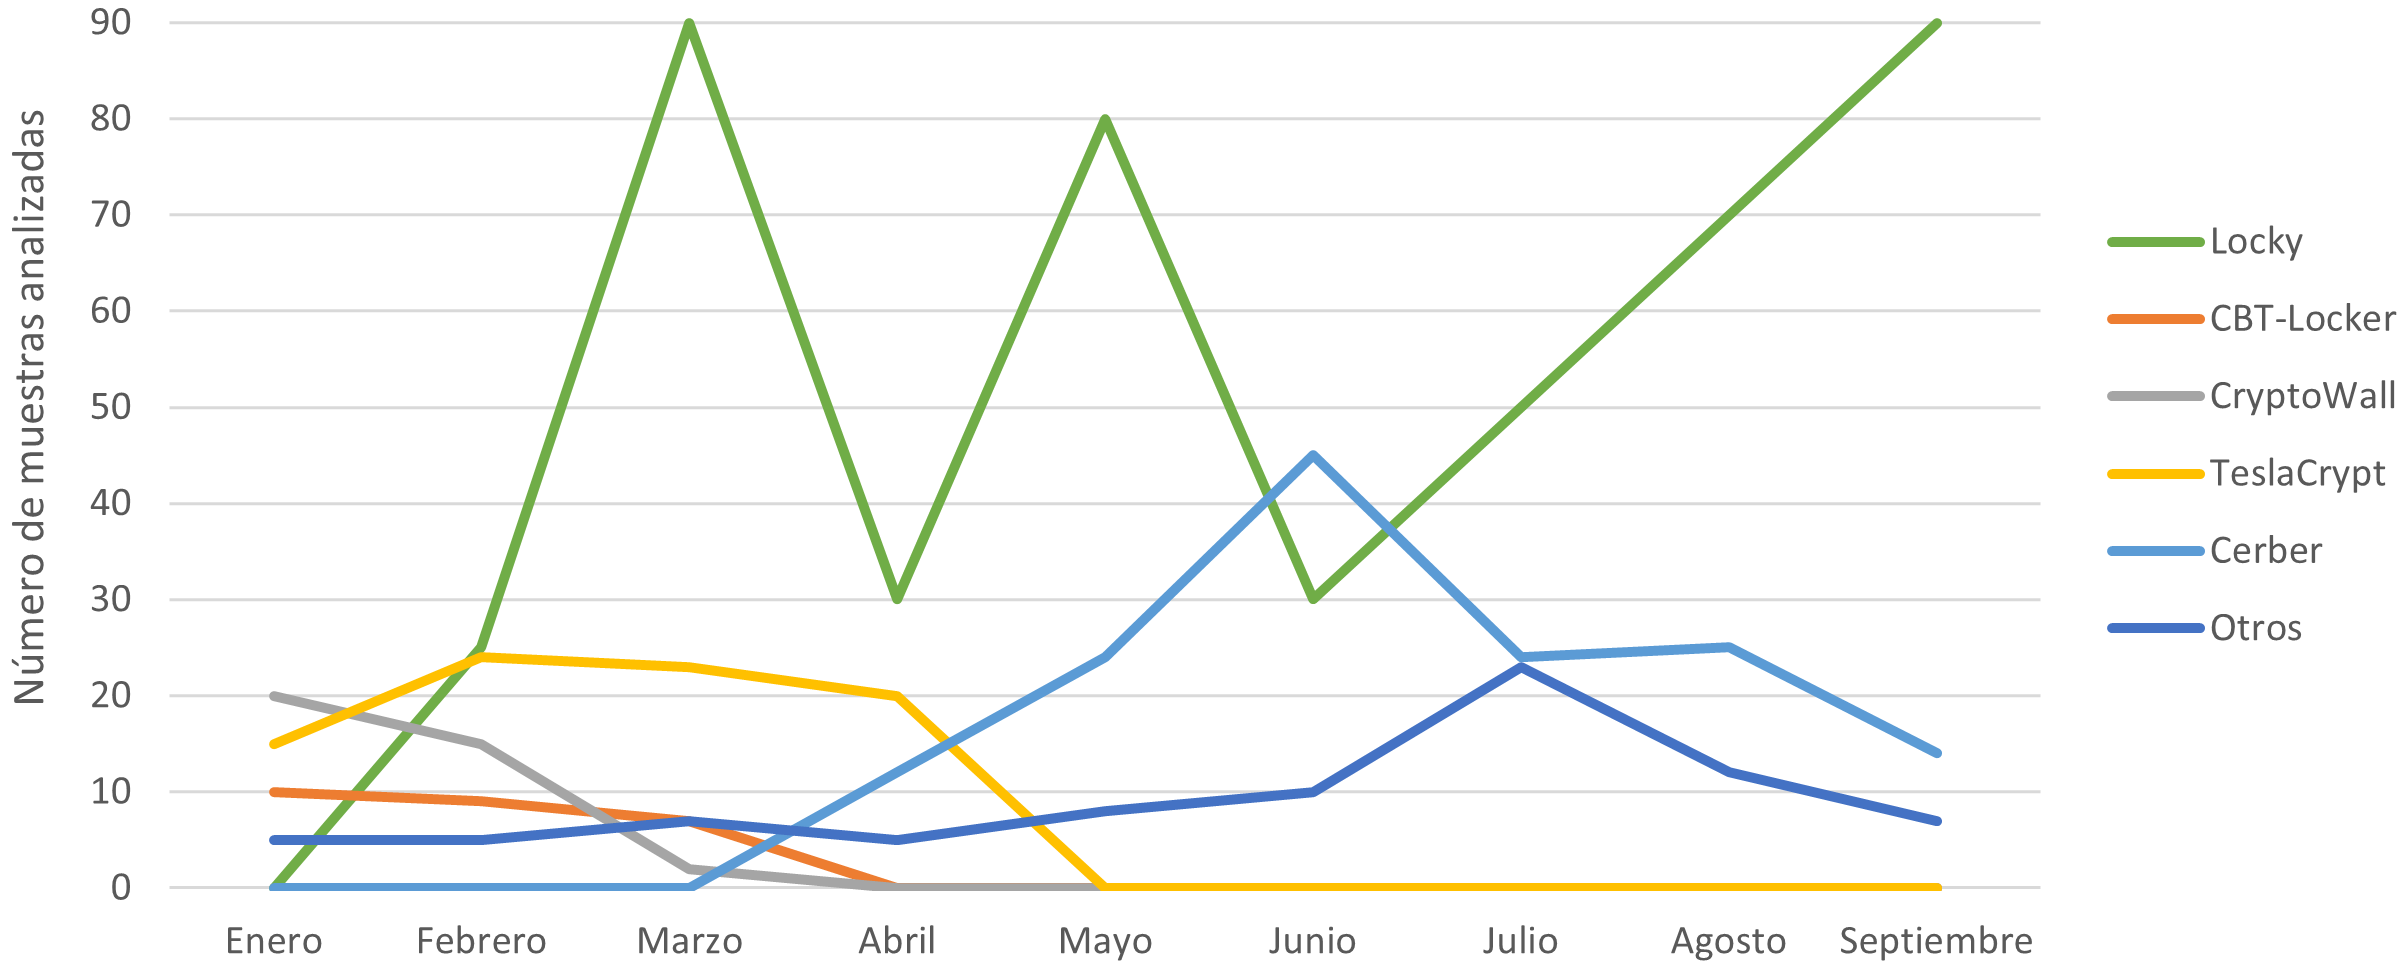
\includegraphics{images/phisme.png}}}
\end{center}
\caption{Familias de ransomware más observadas desde enero hasta septiembre de 2016.}
\label{fig:imphish}
\end{figure}% Marina

%En comparación con las 29 familias de ransomware descubiertas en 2015, en 2016 este número aumentó un 752\%, llegando a 247 en 2016. Los delincuentes recaudaron alrededor de \$1 billón como resultado de atacar a grandes empresas y organizaciones que no tenían copias de seguridad de sus datos, por lo que tuvieron que pagar los rescates \cite{58}. 
%Además, el ransomware continuó su evolución añadiendo nuevas características como contadores para realizar el pago (el rescate se hacía mayor según disminuía) o la propagación por ordenadores mediante la red. Locky, Petya y SamSam fueron las familias más notables descubiertas.

%En 2016 apareció el primer ransomware que atacaba a sistemas Mac \cite{59} y también el primer ransomware llamado ZCryptor que se propagaba automáticamente por los dispositivos conectados a una misma red \cite{60}. Los expertos decían que el 2016 iba a ser un año clave para el ransomware, pero no sabían que lo peor estaba por llegar. 

El año 2017 se consideró por muchos expertos como el ``año de oro del ransomware'', ya que el ataque del ransomware WannaCry fue una epidemia global que sucedió en mayo de ese año. Este ransomware cifraba los archivos de los usuarios, pidiendo \$300 en \textit{bitcoins} por el rescate, y posteriormente esta cifra aumentó hasta los \$600. El 12 de mayo de 2017, WannaCry atacó a sus primeras víctimas en España, en concreto la empresa Telefónica. Días después, el número de usuarios infectados fueron alrededor de 230.000 en más de 150 países, convirtiendo a WannaCry en el mayor ataque de ransomware de la historia. 
Su rápida propagación es debido a que es gusano criptográfico, capaz de replicarse y propagarse automáticamente, aprovechándose de una debilidad en el sistema operativo Microsoft Windows. %siendo capaz de vulnerar cortafuegos y hasta redes privadas virtuales (\gls{VPN}), utilizando herramientas que supuestamente fueron desarrolladas por la Agencia de Seguridad Nacional de los Estados Unidos. 
Este ransomware causó serios daños a bancos, al transporte público, a universidades y a los servicios nacionales de salud, siendo los de Reino Unido los más afectados con costes de alrededor de 92 millones de libras y más de 19.000 citas canceladas \cite{62}.
Además, WannaCry fue el primer ransomware que atacó a los dispositivos \gls{IoT}, en específico a 55 cámaras de tráfico \cite{65}. En definitiva, WannaCry tuvo un impacto importante y se estima que causó pérdidas de alrededor de \$4 billones en todo el mundo \cite{61}.

%Los ataques costaron alrededor del mundo una cifra de 5 billones de dólares, 4 de ellos recaudados por WannaCry, un malware con capacidad para expandirse por las redes, que soporta 27 lenguajes diferentes \cite{ransommasive}.

En 2018 hubo una disminución en los ataques de ransomware. Según los informes publicados por Kaspersky \cite{63} y Malwarebytes \cite{64}, la infección por ransomware cayó un 30\% en todo el mundo, aunque aumentó el número de ataques dirigidos a organizaciones específicas y a dispositivos \gls{IoT}. Estos ataques fueron perpetrados por nuevas variantes de ransomware más sofisticadas, como Ryuk y SamSam. Ryuk atacó a empresas que no se podían permitir periodos de inactividad, como periódicos diarios \cite{66} y una empresa de agua de Carolina del Norte que luchaba contra las secuelas del huracán Florence \cite{67}. %Una característica peligrosa de Ryuk es que puede desactivar la opción restaurar sistema de Windows, lo que dificulta aún más la recuperación de datos cifrados sin pagar un rescate. Las demandas de rescate fueron altas, ya que atacaron empresas con alto valor económico.
SamSam atacó a organizaciones de salud, de educación y de gobierno, explotando el protocolo \gls{RDP} mediante ataques de fuerza bruta y cifrando todos los archivos del sistema. Se estima que el creador de este ransomware ganó alrededor de \$6 millones, ya que atacó a organizaciones tan grandes como el gobierno de Atlanta, que terminó pagando el rescate \cite{9}.

En 2019 se mantuvo la tenencia de lanzar ataques contra organizaciones con gran poder económico y Ryuk siguió siendo un ransomware muy popular entre los criminales junto con Sodinokibi. Sodinokibi o REvil, una variante de GandCrab, fue responsable del cierre de más de 22 pequeñas ciudades de Texas \cite{68} y del ataque a una compañía de cambio de divisas llamada Travelex en la víspera de año nuevo. %Este ataque supuso el cifrado de toda la red de la empresa y el robo de datos personales, incluyendo números completos de tarjetas de crédito de clientes.
Los delincuentes pidieron \$6 millones por el rescate, pero la empresa no pagó \cite{69}.

La Figura \ref{fig:imavg}, creada con datos sacados de un estudio realizado por Crypsis \cite{70}, muestra la media de los rescates pedidos por los delincuentes en los Estados Unidos. Se aprecia un incremento del 140\% entre los dos años, 2018 y 2019 y esto evidencia la situación de que cada vez el ransomware es más sofisticado y ataca a objetivos más grandes con el objetivo de obtener mayores cantidades de dinero. El aumento de la cuantía de los rescates también es debido a que las compañías pagaban a los criminales, lo que les incentivaba a atacar más. En 2018 el 38\% de las empresas afectadas pagaron la suma exigida y en 2019 el 45\%.
%\change{Las gr\'aficas no deben tener el título insertado. colocar el texto de las figuras en times new roman hay texto} 
\begin{figure}[h!]
\begin{center}
{\scalebox{.7}{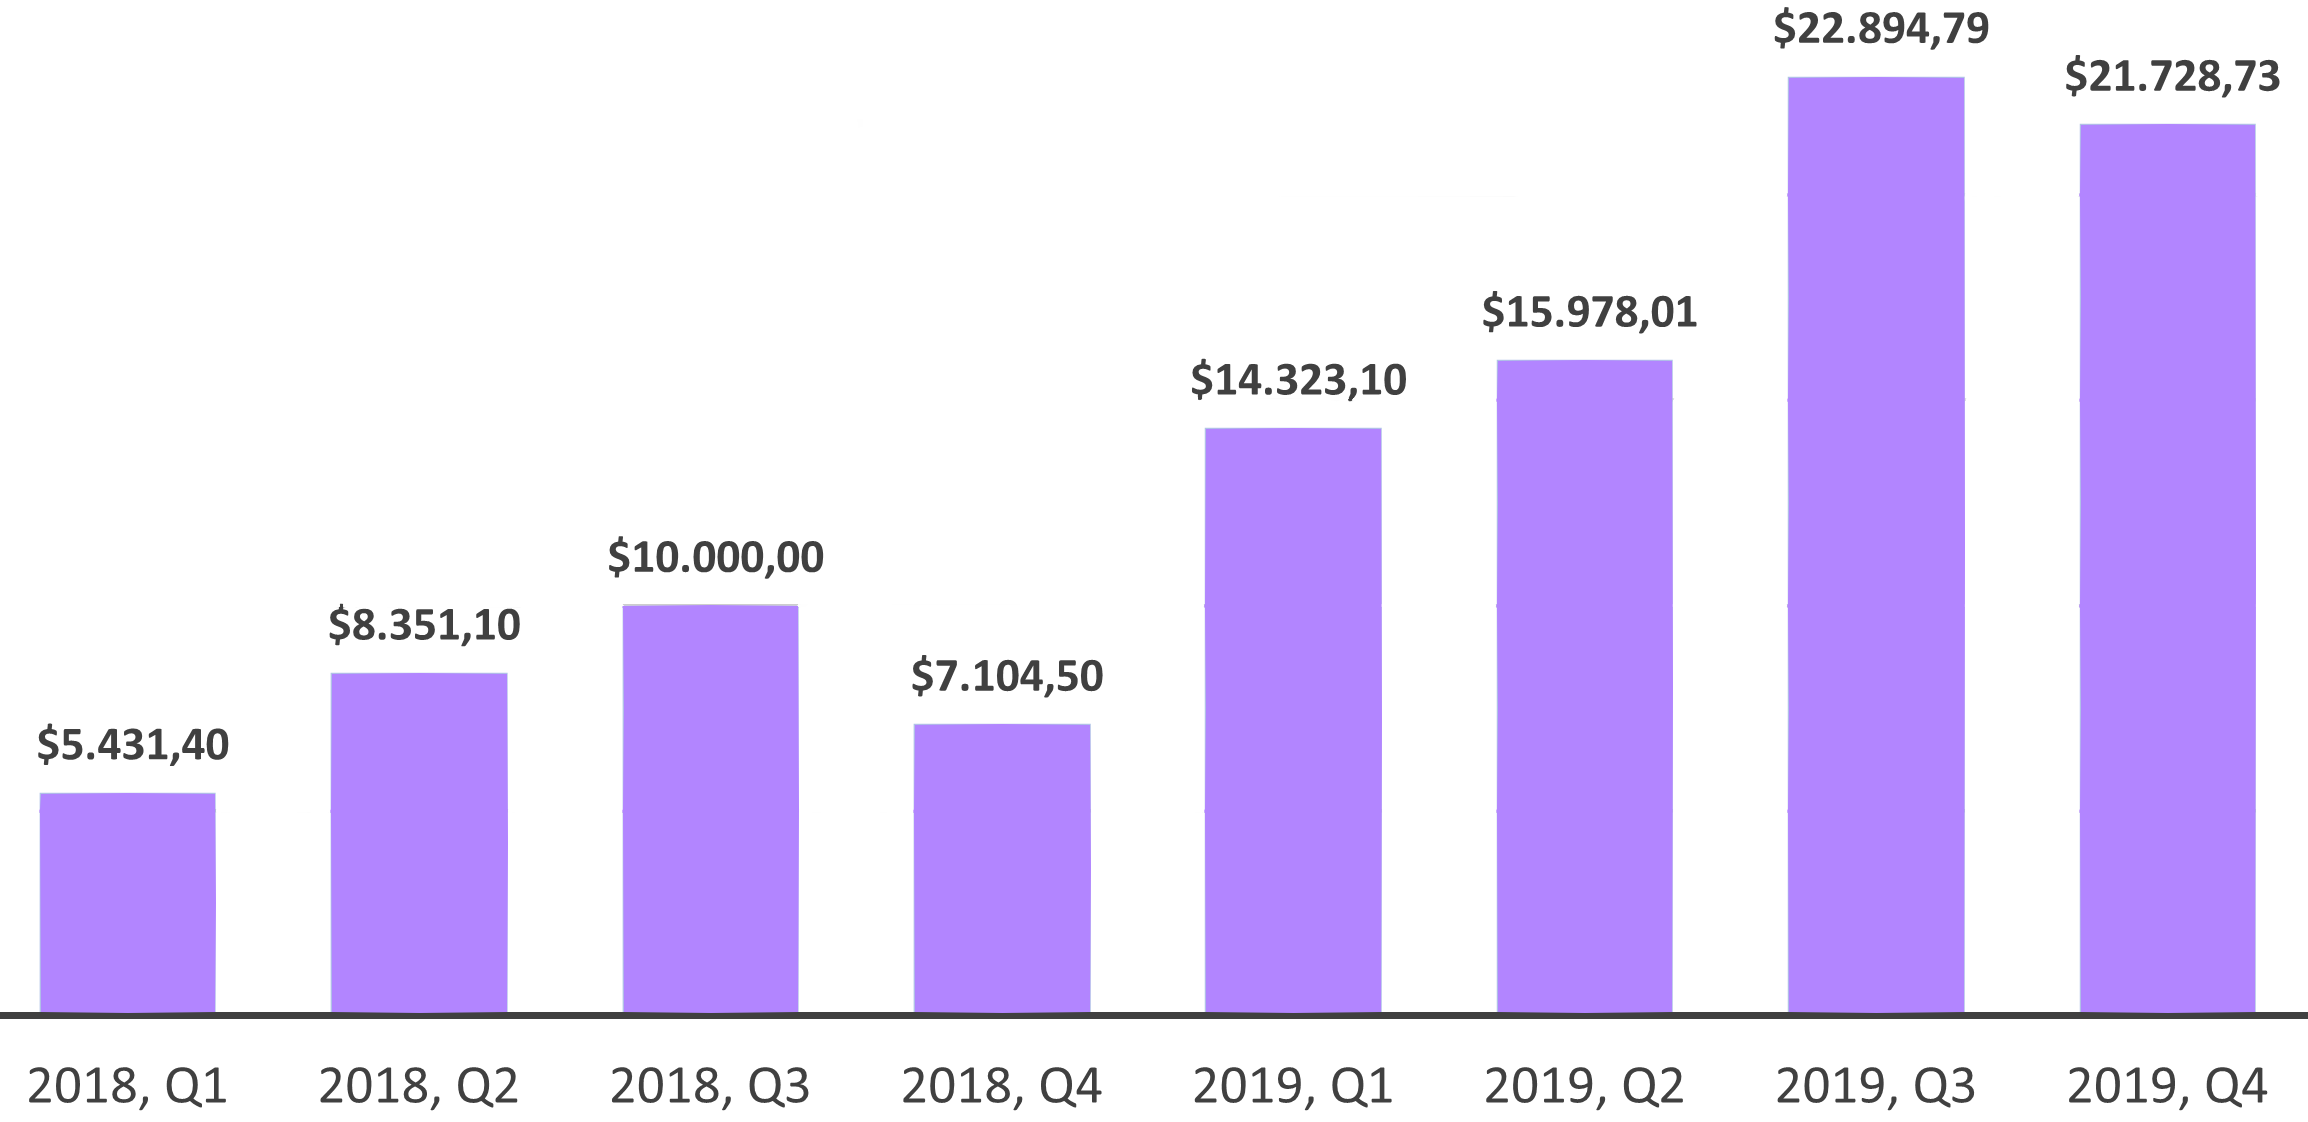
\includegraphics{images/crypsis.png}}}
\end{center}
\caption{Media de la cantidad de dinero que los \textit{hackers} pedían por los rescates en los Estados Unidos (2018-2019).}
\label{fig:imavg}
\end{figure}

En 2020 el ransomware continúa la tendencia de los ataques dirigidos a organizaciones, pero empleando el método de la doble extorsión. No solo cifran y roban los datos, también amenazan con publicarlos si no se pagaba el rescate. Esto supuso una seria amenaza especialmente para las organizaciones más grandes que tienen información altamente confidencial en sus sistemas, y dichos ataques les podrían costar mucho dinero y dañar su reputación e imagen \cite{71}. Maze es un ejemplo de una familia de ransomware que utilizó esta táctica, distribuyéndose de diferentes maneras. La principal fue a través de campañas de \textit{spear-phishing} que instalaban un malware llamado \textit{Cobalt Strike}, pero también infectaba a sistemas con credenciales débiles de \gls{RDP} mediante la explotación de servicios vulnerables de internet para penetrar las redes \cite{25}.
%Gran parte del año 2020 estuvo dominado por las noticias del \gls{COVID-19} y los delincuentes no dudaron en aprovecharse de la crisis y del miedo de las personas. Sucedieron oleadas de campañas de correos electrónicos con archivos maliciosos adjuntos y ransomware dirigido a organizaciones debilitadas o quebradas.
Un estudio realizado por Sophos \cite{38} muestra datos con los que se ha realizado la Figura \ref{fig:imsoph}, que indica el volumen de menciones sobre el \gls{COVID-19} en correos no deseados después de haber sido declarado como pandemia global por la \gls{OMS}.

\begin{figure}[h!]
\begin{center}
{\scalebox{.75}{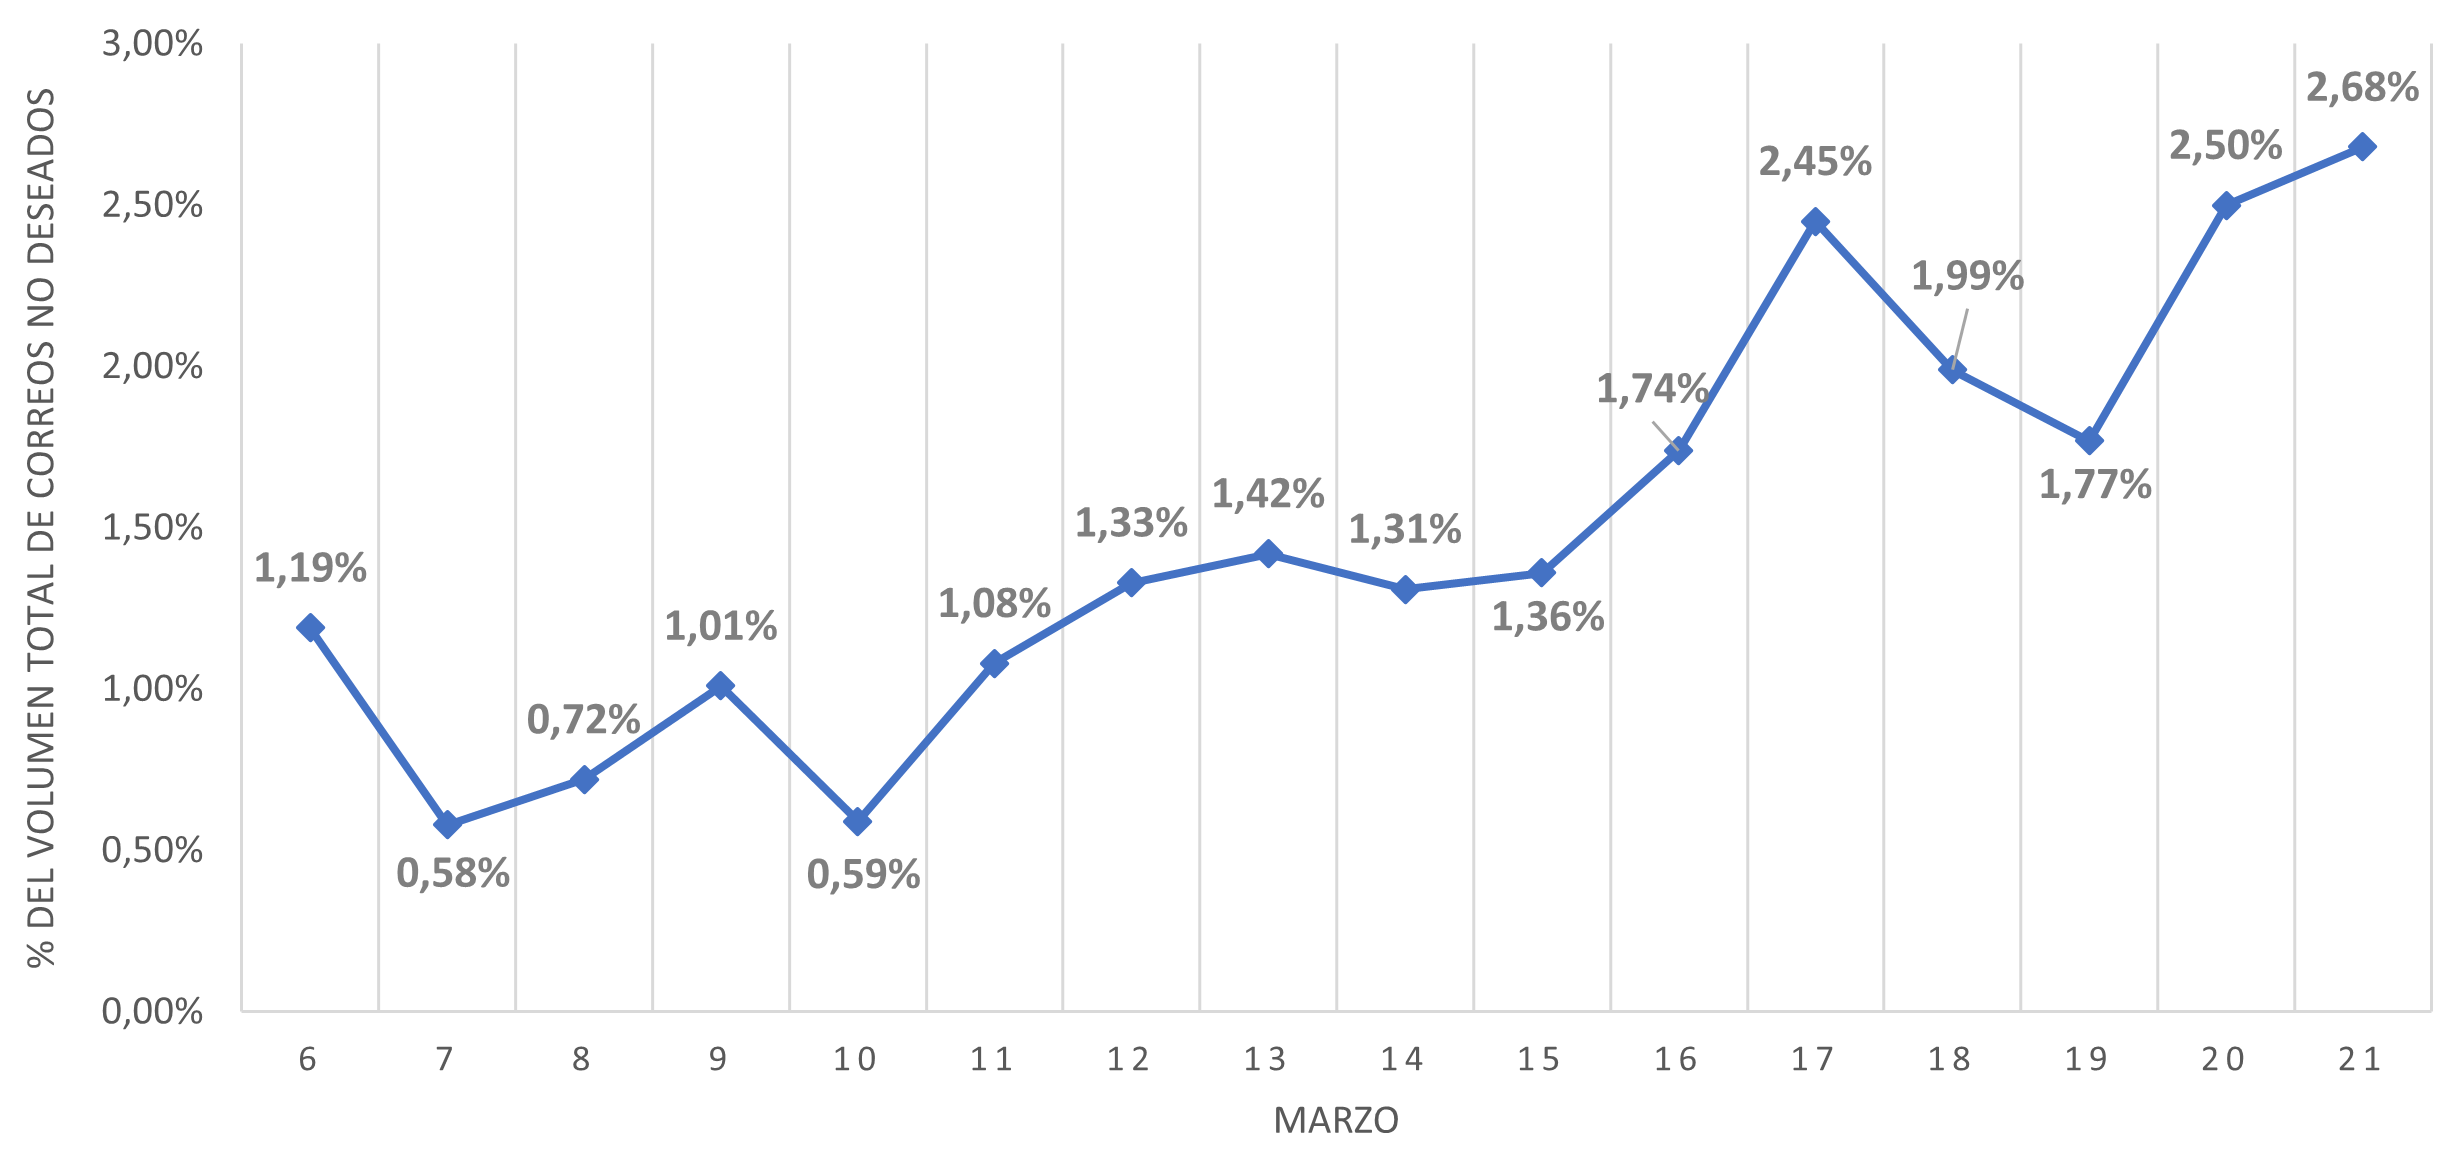
\includegraphics{images/covid_sophos.png}}}
\end{center}
\caption{Volumen de menciones del COVID-19 en correos no deseados de todo el mundo en el mes de Marzo.}
\label{fig:imsoph}
\end{figure}

\begin{comment}

Los expertos pronosticaron un aumento de ataques de ransomware para el 2021 y unas pérdidas mayores para las empresas que están siendo atacadas más y más cada año.
Muchas de las compañías afectadas por ransomware dicen que han experimentado tiempos de inactividad y pérdidas de datos personales, lo que resultó en perdidas millonarias como se puede ver en la Figura \ref{fig:imsafety} creada con los datos sacados de un estudio realizado por SafetyDetectives \cite{72}.

\begin{figure}[h!]
\begin{center}
{\scalebox{.2}{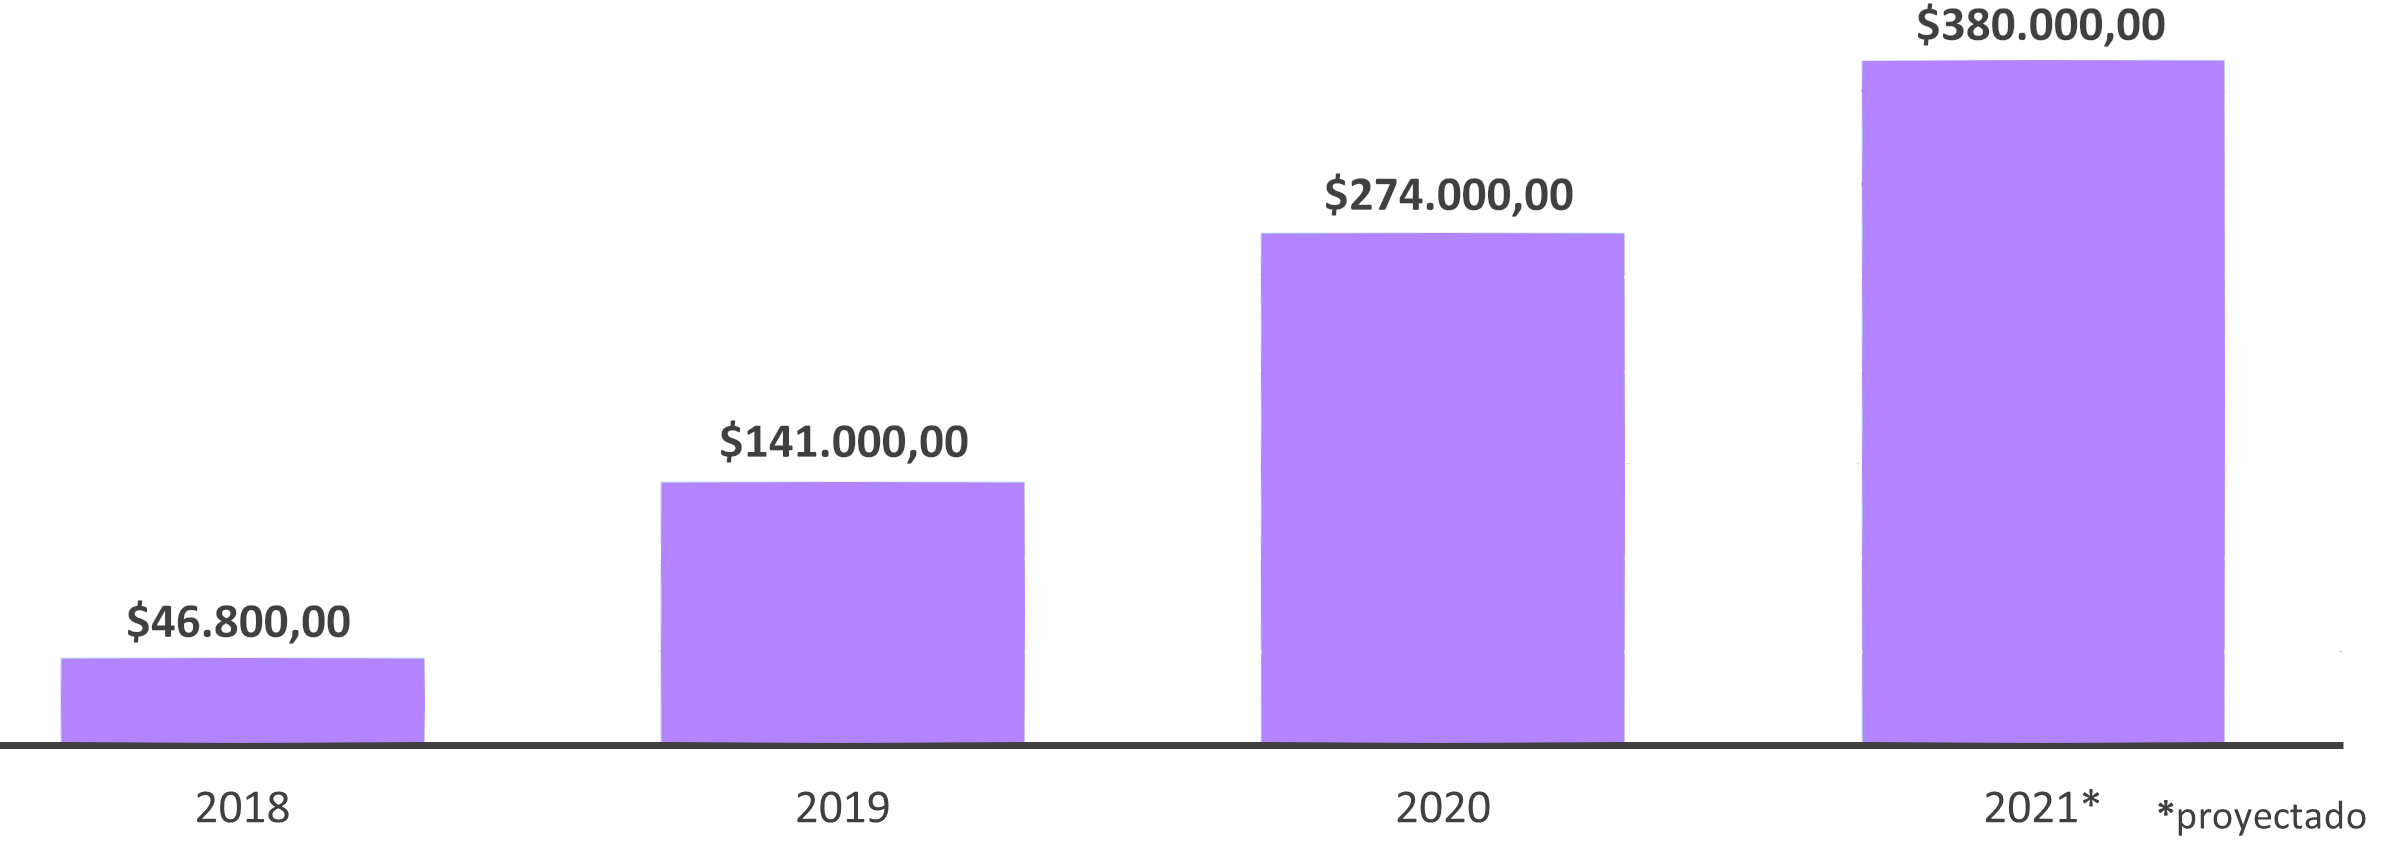
\includegraphics{images/safety_costes.png}}}
\end{center}
\caption{Coste promedio causado por tiempos de inactividad en las empresas afectadas por ransomware.}
\label{fig:imsafety}
\end{figure}


\end{comment}


El primer ransomware del 2021 es Babuk, apareciendo por primera vez en enero y afectando especialmente a empresas de España y Chile. Este ransomware usa su propio esquema de cifrado llamado \textit{ChaCha8}, una variante de Sodinokibi, usando criptografía de curva elíptica. Los precios del rescate oscilan entre \$65.000 y \$85.000 \cite{73}.

En vista de la constante evolución del ransomware, es evidente que las organizaciones son las que están en peligro constante debido a su alto poder económico y a su necesidad de estar operativas todo el tiempo. No se pueden permitir que un ransomware bloquee sus sistemas y tienden a pagar los rescates, sin darse cuenta de que eso solo incentiva a los criminales y no hay certeza de que lleguen a recuperar todos sus archivos y datos afectados. Los criminales pueden intentar negociar y sacar más dinero al ver que la empresa está dispuesta a pagar, por lo que la prevención es clave y la única solución factible. 

La Figura \ref{fig:crono} muestra la cronología de la evolución del ransomware explicada anteriormente, con los ransomware más destacados y los años en los que surgían.
\newpage
\begin{figure}[h!]
\begin{center}
{\scalebox{.4}{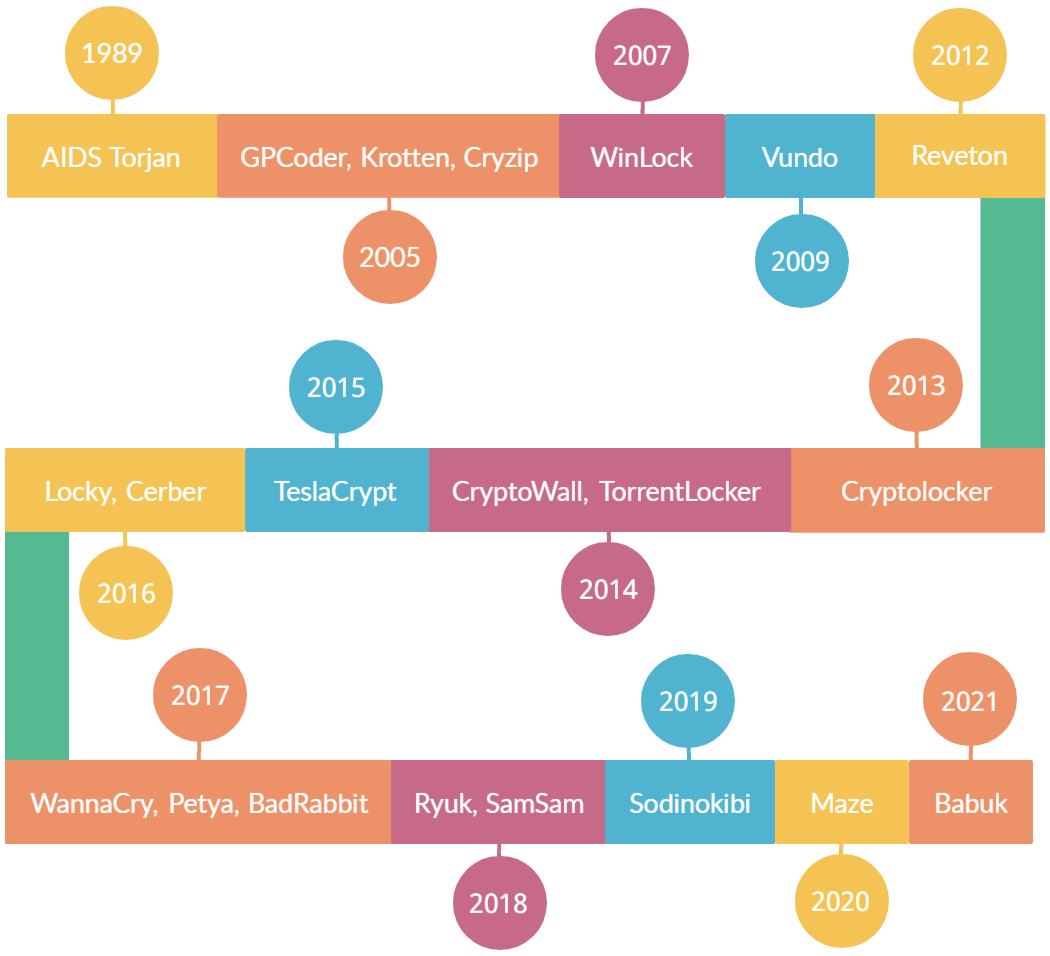
\includegraphics{images/ransomware_timeline.png}}}
\end{center}
\caption{Cronología de la evolución del ransomware.}
\label{fig:crono}
\end{figure}


\section{Tipos de Ransomware}\label{sec:2-4}

\noindent Se identifican dos tipos de ransomware dependiendo de la técnica que utilicen para atacar los sistemas \cite{ransommasive}:

\begin{enumerate}
    \item \textbf{Lockscreen}: Se caracterizan por que bloquean el acceso al sistema a través de la pantalla. En ella se muestra un mensaje indicando que el equipo ha sido infectado y el rescate que deben pagar e imposibilitan al usuario a salir de dicha pantalla.
    Este tipo de ransomware solamente bloquea el acceso a la interfaz del ordenador pero no afecta los archivos. Por lo tanto, existe la posibilidad de eliminar el ransomware y mantener todos los archivos intactos \cite{80}.
    \item \textbf{Filecoder}: Estos ataques cifran archivos del usuario impidiendo el acceso de los usuarios  a su información. Para obtener la clave de descifrado, los usuarios deberán pagar un rescate. Criptolock es el más famoso \cite{79}.
    
\end{enumerate}


En los últimos años además de estos dos tipos han surgido otras variedades que, aunque similares, tienen sus peculiaridades y es importante diferenciarlos para poder comprender su comportamiento y clasificarlos de mejor manera \cite{81}:

\begin{itemize}
\item \textbf{Virus de la policía}: Este ransomware es similar al \textit{Lockscreen}, ya que bloquea el acceso al equipo. La diferencia es el mensaje que muestra al arrancar el sistema, siendo este un mensaje falso de la policía, informando al usuario que se ha detectado accesos a páginas ilegales y que tiene que pagar una multa. 
\item \textbf{Wiper}: Paredico al Filecoder pero más destructivo, ya que bloquea definitivamente el acceso a los archivos y posteriormente los elimina.
\item \textbf{Scareware}: Se hace pasar por un detector de amenazas utilizando ventanas emergentes para informar al usuario sobre supuestos problemas encontrados en su equipo. En lugar de exigir dinero, este ransomware presiona al usuario para que compre un software antivirus falso para resolver todos los problemas instantáneamente. Si el usuario paga e instala el supuesto antivirus, este actuará como malware y recopilará información del equipo y datos personales del usuario \cite{84}.
\item \textbf{Hoax ransomware}: Este ransomware es similar a un Filecoder, pero no cifra ningún archivo ni bloquea el equipo. Simplemente utiliza técnicas de ingeniería social para asustar al usuario y hacerle pagar un rescate falso.
\item \textbf{Leakware}: También llamado \textit{doxware}, este ransomware amenaza al usuario con la publicación de su información personal, como datos confidenciales y conversaciones almacenados si no paga un rescate. Este ransomware es peligroso para las empresas, ya que puede revelar información comprometedora \cite{85}.
\item \textbf{Ataque oculto}: Sucede cuando un usuario simplemente navega a través una página web vulnerada por un \textit{hacker} \cite{82}.
\item \textbf{Dropper}: Infecta al sistema al instalar un programa que en realidad es malware disfrazado, y esto se denomina instalador (\textit{dropper}) de malware. Bad Rabbit, un ransomware que surgió en 2017, se propagó haciendo uso de una solicitud falsa para instalar Adobe Flash, que en realidad era un instalador de malware \cite{83}.
\end{itemize}

Hay otros tipos de ransomware que no tienen un nombre en concreto, pero es conveniente mencionarlas. La reescritura del \gls{MBR} antes de cifrar los datos es una estrategia inusualmente agresiva que usa el ransomware CoViper, y el \gls{FDE} lo realiza el ransomware Mamba. Petya hace algo similar, pero solo cifra la \gls{MFT}, por lo que los datos en si no se ven afectados \cite{82}.


Finalmente, cabe mencionar otras técnicas de extorsionar a las víctimas \cite{ransommasive}:

\begin{enumerate}
    \item \textbf{Scareware}: Este tipo de malware funciona convenciendo a las víctimas para comprar artículos que no necesitan mediante alertas de seguridad falsas.
    
    \item \textbf{Extorsión DDoS}: Puede ser considerado \textit{blackmail} cuando los atacantes solicitan dinero por no realizar un ataque distribuido de denegación de servicio.
    
    \item \textbf{Extorsión por datos comprometidos}: El ciberdelincuente amenaza a la víctima con exponer datos sensibles públicamente a no ser que éste pague un rescate.
\end{enumerate}


\section{Familias de Ransomware}\label{sec:2-5}
\noindent A continuación se listan algunas de las familias más peligrosas y con mas impacto \cite{histRansom} \cite{smartech}:
\begin{itemize}
    
    \item \textbf{Petya}: Tiene dos variantes, una de 2016 y otra, llamada NotPetya, que apareció en 2017. Una vez ejecutado, Petya sobrescribe el sistema de arranque, posteriormente cifra la tabla de ficheros maestros, provocando que Windows sea incapaz de localizar los ficheros almacenados. Posteriormente se reinicia el ordenador, y Petya evita que Windows arranque con normalidad y muestra un mensaje de extorsión como el que se puede observar en la Figura \ref{fig:im5}, procedente del análisis de Cuckoo Sandbox de una muestra realizada en este estudio.
    NotPetya es muy peligroso puesto que puede ser propagada con intervención humana y las claves de cifrado son generadas aleatoriamente y destruidas, lo que hacen que la recuperación de los datos sea imposible \cite{ransommasive}.
    \begin{figure}[htb]
    \begin{center}
    {\scalebox{.5}{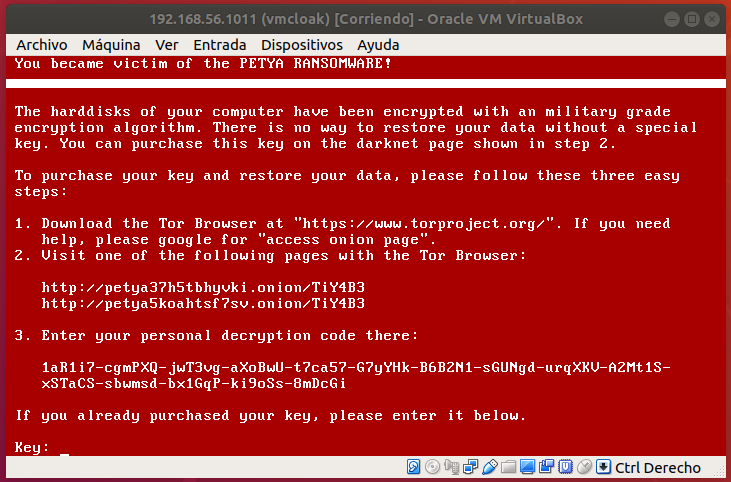
\includegraphics{images/Petya.png}}}
    \end{center}
    \caption{Aviso de extorsión del ransomware Petya}
    \label{fig:im5}
    \end{figure}
    
    \item \textbf{Locky}: Los usuarios se infectan debido a un correo electrónico. Utiliza macros y archivos de \textit{script} para cifrar archivos cuando se abre un documento. Al ejecutarse el \textit{script}, los archivos cifrados se renombran y Locky muestra al usuario una nota de rescate, configurándola como fondo de pantalla. Locky utiliza un algoritmo de cifrado \gls{RSA}-2048+\gls{AES}-128 para cifrar archivos, discos duros e incluso dispositivos extraíbles. Locky ataca a máquinas con base Windows, eliminando el sistema Windows \textit{Shadow Volume Copy} para prevenir cualquier posible recuperación de archivos por parte del usuario.
    
    \item \textbf{SamSam}: Es usado para atacar a una organización, después de haber realizado un estudio y reconocimiento de sus sistemas IT, para reconocer alguna vulnerabilidad en la red o equipos. Afecta a una máquina y se propaga por red a todos las conectadas. Se diferencia a otras familias porque no utiliza técnicas de ingeniería social como correos electrónicos de \textit{spam} o \textit{phising}, sino que los atacantes realizan ataques de fuerza bruta contra las contraseñas débiles para ganar acceso a la red de la organización tras el estudio previamente comentado \cite{ransommasive}. 
    
    \item \textbf{CryptoWall}: Se trata del sucesor de CryptoLocker. Su objetivo son máquinas de base Windows, y se propaga mediante e-mails maliciosos y kits de \textit{exploits} como Nuclear o Angler. Una vez ejecutado en el equipo, escribe su propio registro de auto-arranque, de modo que es resistente a los reinicios. Elimina los sistemas de restauración y procede a cifrar los archivos mediante el algoritmo \gls{RSA}-2048. Su versión más reciente, CryptoWall 4.0 usa un esquema de comunicación con la red \gls{TOR} a través de un servidor \textit{proxy} externo \cite{ransommasive}, como se puede observar en la Figura \ref{fig:imcryp}.
    \begin{figure}[htb]
    \begin{center}
    {\scalebox{.85}{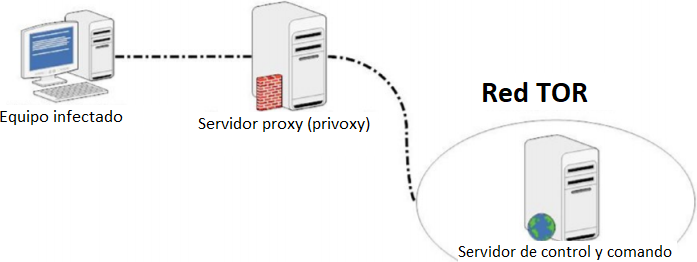
\includegraphics{images/cryptowall.png}}}
    \end{center}
    \caption{Esquema de red de un ataque con Cryptowall}
    \label{fig:imcryp}
    \end{figure}
    
    \item \textbf{CryptXXX}: Familia de ransomware de cifrado que ataca a sistemas operativos Windows. No cifra únicamente los archivos, sino que también ejecuta otro malware de robo de información, como por ejemplo credenciales de VPN, \textit{cookies} o incluso \textit{bitcoins} del ordenador de la víctima y es enviado de nuevo al servidor de control y comando. Utiliza el algoritmo de cifrado \gls{RSA}-4096 y añade la extensión``.crypt'' al nombre del fichero. Posee un sistema anti-sandboxing y anti-analisis \cite{ransommasive}.
    
    \item \textbf{Cerber}: Se diferencia al resto porque es capaz de emitir por los altavoces del dispositivo mensajes de alerta de infección del malware. Incluye ataques a plataformas \textit{Cloud} y \textit{Windows Scripting} y ataques \gls{DDoS}. No solo ataca a máquinas de usuarios individuales, sino que también ha llegado a cifrar bases de datos enteras de empresas.
    
    \item \textbf{Jigsaw}: Debe su nombre a que utiliza como imagen de bloqueo de pantalla al protagonista de la película \textit{Saw}. Infecta archivos de manera exponencial cuanto más tiempo pase sin que la víctima pague el rescate. 
    Posee una característica peculiar que habilita un ``chat'' que ayuda al usuario a pagar para recuperar sus datos.
    
    \item \textbf{CryptoLocker}: Es el primero en utilizar \textit{bitcoin} como moneda de rescate. Accede al sistema utilizando técnicas de ingeniería social, mediante correos electrónicos de empresas de paquetería. Se trata de un ransomware que combina las técnicas de Lockscreen y CriptoLocker.
    
    \item \textbf{WannaCry}: Se diferencia por su éxito de infección, más de 300.000 equipos en más de 150 países fueron afectados por este ransomware debido a una vulnerabilidad de Windows que permite a un atacante remoto ejecutar código arbitrario \cite{exploit}. La dificultad de protegerse contra WannaCry reside en que usa un componente de gusano, que provoca que el ataque sea mucho más efectivo y se necesiten mecanismos de defensa que puedan reaccionar en tiempo real \cite{Akbanov2019}.
 
    \item \textbf{HDDCryptor}: Bloquea la máquina además de afectar a recursos compartidos en la red como impresoras, puertos y archivos a través de \textit{Server Message Block}. Ataca tanto a usuarios individuales como a empresas, y un ejemplo conocido es Mamba.
    
    \item \textbf{Crysis}: También conocido como Dharma, es un ransomware que utiliza ataques de fuerza bruta para propagarse. En 2017, Dharma consiguió que se duplicaran este tipo de ataques por todo el mundo. Esta familia se ha encontrado en 123 países, concentrándose el 60\% de los ataques en 10 países, entre los cuales España ocupa la segunda posición \cite{CcnCert}. 
    
\end{itemize}

En el Anexo \ref{anexo-1} se presenta una lista extendida de las familias de ransomware más conocidas \cite{7}. 

\section{Métodos de Propagación}\label{sec:2-6}
\noindent En esta sección se exponen los diferentes vectores de ataque usados por los creadores de ransomware para invadir los sistemas víctimas \cite{ransommasive}.


\begin{itemize}
    \item \textbf{Ataque de fuerza bruta}: Este ataque sucede cuando los criminales emplean el \gls{RDP} y técnicas para probar una gran variedad de combinaciones de contraseñas, con el objetivo de revelar las credenciales del usuario y así lograr acceso a su sistema \cite{78}.  
    
    \item \textbf{Auto-propagación}: Es la propagación del ransomware de un sistema infectado a otro, difundiendo archivos infectados a todos los contactos disponibles en esa máquina. Antes de iniciar el proceso de cifrado, se expande rápidamente para aumentar sus posibilidades de infectar otros ordenadores \cite{29}.

    \item \textbf{Dispositivos \gls{USB}}: Aunque se trate de un método de propagación primitivo, los cibercriminales siguen utilizándolo para realizar ataques a sistemas. Requiere el acceso físico a algún puerto donde poder conectar el dispositivo ejecutor, aunque existe alguna técnica como esparcir memorias \gls{USB} por diversos lugares con la expectativa de que algún usuario los conecte.
    
    \item \textbf{Drive-by-Downloads}: Los atacantes comprometen sitios web legítimos e incrustan código malicioso en sus páginas, como código \textit{JavaScript}. Este código malicioso realiza publicidad maliciosa, redirecciones engañosas, ataques \gls{XSS} u otros ataques en secreto, sin que el usuario sepa que su sistema está siendo infectado \cite{46} \cite{47}.

    \item \textbf{E-mail}: Es la manera más utilizada, con un 59\%, según un estudio de IBM de 2017 \cite{IBMstats}. Cuando los descuidados usuarios descargan y abren el contenido malicioso, el sistema se infecta de inmediato. También pueden contener \gls{URL} a páginas web maliciosas que infectan el computador. Suelen realizarse mediante campañas de \textit{spam}, e-mails no solicitados enviados a grandes grupos de personas, con el objetivo de realizar promociones. Se trata de algo convincente puesto que, los mensajes de \textit{spam} se contabilizaban como el 53.5\% del tráfico mundial en 2018 \cite{statista}. La técnica más utilizada es el \textit{phising}. Se basa en realizar campañas de \textit{spam} usando el mismo formato que alguna compañía legítima en sus comunicaciones para recaudar información de la víctima. 

    \item \textbf{Botnets troyanos}: El ransomware también puede llegar a un sistema a través de otro malware. Este es el caso de los \textit{Botnets}, que son una red de robots que se ejecutan de manera automática y autónoma. El término \textit{Botnet} surge con una combinación de dos palabras, ``bot'' de robot y ``net'' de red en inglés. Estos robots controlan a los equipos que infectan para que realicen varias tareas, tales como: atacar a otros ordenadores, enviar correos electrónicos no deseados a los contactos del usuario, entregar ransomware, instalar \textit{spyware} y otras actividades maliciosas similares \cite {45}. La Figura \ref{fig:im8} muestra un diagrama de acción de una \textit{Botnet}.

    \begin{figure}[htb]
    \begin{center}
    {\scalebox{.7}{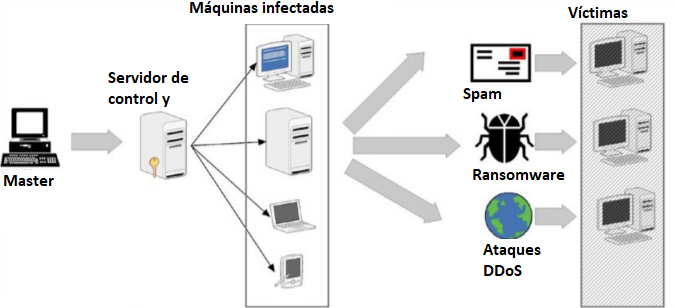
\includegraphics{images/botnet.png}}}
    \end{center}
    \caption{Diagrama de acción de un botnet}
    \label{fig:im8}
    \end{figure}

    \item \textbf{Explotar vulnerabilidades de servidores}: Los criminales explotan las vulnerabilidades del software que se ejecuta en servidores para obtener acceso a la red de una organización y difundir su malware a través de ella \cite{29}.

    \item \textbf{Kits de Exploit}: 
    %Los \textit{exploit kits} aprovechan las vulnerabilidades del software de servidores web para instalar malware, inyectando \textit{iframes} (componentes de un elemento HTML que permiten incrustar contenido) en las páginas web alojadas en ellos. Los \textit{iframes} redirigen a los usuarios que navegan por esos sitios a los \textit{exploit kits}. Se ha visto un aumento del uso de estos kits, especialmente uno llamado \textit{Angler} \cite{30}. Este kit roba las contraseñas del equipo y luego lo infecta con ransomware.
    Se definen como plataformas web que permiten ejecutar \textit{exploits} de manera semi-automática mediante la detección de vulnerabilidades en el sistema operativo o la aplicación víctima y comparándolas con las almacenadas en el kit. Se componen de cuatro partes:
    \begin{enumerate}
        \item \textbf{Página de destino}: Contiene el código responsable para escanear las vulnerabilidades a explotar.
        \item \textbf{Puerta}: fragmento de código que recibe la información de la página de destino y decide si continuar con el ataque o no, según los criterios predefinidos.
        \item \textbf{Exploit}: Explota las vulnerabilidades previamente detectadas ejecutando algún tipo de código malicioso en la máquina víctima para poder acceder a ella.
        \item \textbf{Carga}: Tras haber accedido mediante las vulnerabilidades, el kit de \textit{exploit} envía la carga, algún tipo de malware o algún mecanismo que lo descargue, para realizar el daño real.
    \end{enumerate}
    
    \item \textbf{Malvertising}: Anuncios maliciosos distribuidos a través de páginas web confiables por atacantes que compran espacios publicitarios. Los usuarios que acceden a esas páginas ni siquiera tiene que hacer clic en el anuncio en algunos casos, ya que simplemente cargar la página web que aloja la publicidad maliciosa provocará una infección \cite{44}. Esto era muy común cuando los sitios web usaban Adobe Flash para reproducir anuncios animados \cite{43}.

%La publicidad maliciosa es un tipo de ataque por el que se abusa de canales de publicidad legítimos para propagar malware mediante la inyección de código dentro de los anuncios y las plataformas web. En la práctica, los anuncios maliciosos pueden aparecer como una ventana emergente para llamar la atención del usuario. Si éste hace click en dicho anuncio, se descarga automáticamente el malware.
    
    \item \textbf{Macros de Microsoft Office}\label{item:macros}: Son una serie de instrucciones y comandos para automatizar tares en programas de Microsoft Office como Word o Excel. Los cibercriminales distribuyen por la red ficheros de estos programas con macros maliciosas en ellos y, cuando el usuario las abre, la macro ejecuta funciones malignas para la máquina víctima. 

    \item \textbf{Phishing y técnicas de ingeniería social}: El \textit{phishing} es un ciberataque que usa correos electrónicos como arma, siendo el método más efectivo para distribuir ransomware \cite{41}. Su objetivo es recopilar información personal del usuario mediante correos electrónicos o sitios web maliciosos, engañándole para que acceda a un enlace o que descargue un archivo adjunto. Lo que distingue al \textit{phishing} es la forma del mensaje: los atacantes se disfrazan como una entidad confiable, a menudo una empresa o persona real con la que la víctima podría hacer negocios \cite{42}. Otra técnica de ingeniería social usada comúnmente por los delincuentes es engañar al usuario para que descargue un antivirus falso, y al escanear el equipo con este programa, será infectado por el ransomware.

    \item \textbf{Ransomware as a Service}: \gls{RaaS} es un servicio de ventas de paquetes software de ransomware establecido en mercados negros o foros usando un modelo de suscripción. Se trata de una plataforma emergente muy dañina que permite adquirir software malicioso de manera sencilla. Intervienen tres actores: el autor del código, un proveedor de servicios y los agentes que los adquieren, los futuros atacantes.
    
\end{itemize}

\section{Modo de Operación}\label{sec:2-7}
\noindent Los ataques ransomware siguen las siguientes fases desde que se instalan en el equipo víctima hasta que el usuario puede advertir su presencia \cite{ransommasive}:

\begin{enumerate}
    \item \textbf{Infección}: El ransomware es introducido en el sistema mediante las técnicas detalladas en la Sección \ref{sec:2-6}.
    
    \item \textbf{Ejecución}: Si la infección fue satisfactoria, el ransomware se instala en el equipo víctima y se conecta con el \gls{CyC} mediante el protocolo criptográfico \gls{TLS} y le empezará a enviar información de la víctima de forma segura \cite{35}.
    
    \item \textbf{Destrucción del respaldo}: El ransomware realiza una búsqueda de los ficheros de respaldo y los elimina, de manera que el usuario sea incapaz de recuperar sus archivos. En paralelo, el ransomware también elimina las copias de seguridad del sistema y dependiendo del tipo, también podrá eliminar las \textit{shadow volume copies} (instantáneas) del sistema o cambiar los nombres de los archivos, agregando una extensión relacionada con el nombre de la familia del ransomware \cite{29}. 
    
    \item \textbf{Cifrado}: Se establece una conexión segura con el servidor \gls{CyC} para que le proporcione al ransomware una clave simétrica generada aleatoriamente y este empezará a cifrar los archivos del usuario, usando el algoritmo de cifrado asimétrico \gls{RSA}. Este algoritmo usa dos claves diferentes, una pública para el cifrado de los datos y otra privada para el descifrado  \cite{36}. También pueden usar el algoritmo \gls{AES}, siendo \gls{AES}-256 la forma más común \cite{34}.
    
    \item \textbf{Rescate}: El ransomware reproduce un mensaje de extorsión en la pantalla del ordenador de la víctima, estableciendo un coste y un período de tiempo. 
\end{enumerate}

Los atacantes pueden intentar minimizar la detección del ransomware mediante el uso de certificados digitales legítimos, comprados o robados, para intentar convencer a los software antivirus de que el código es fiable y no necesita ser analizado \cite{39}. Aún así, este método podría fallar, ya que este certificado puede ser revocado en cualquier momento por las autoridades pertinentes, por lo que el ransomware debe actuar rápidamente. Para conseguir rapidez y efectividad, el ransomware dispone de un mecanismo que le ayuda a diferenciar qué archivos son los más importantes para robarlos y cifrarlos primero. La importancia de estos archivos se mide viendo lo relevantes que son para el usuario, comparando cuando se accedieron por última vez y cuando se crearon \cite{33}, dónde están ubicados (el directorio ``Documentos'' suele contener archivos importantes) y su entropía \cite{32}. Si la entropía es demasiado alta o baja, es porque el archivo contiene información aleatoria o simplemente relleno, por lo que el ransomware interpretará que el archivo fue generado automáticamente por el sistema y lo descartará \cite{30}. Otro método más comúnmente utilizado para evitar ser detectado es el aumento de los privilegios mediante el uso de \textit{exploits}, permitiendo a los atacantes instalar programas como \gls{RATS} (herramientas de administración en remoto) para cambiar o borrar datos, crear nuevas cuentas con todos los derechos de usuario y lo más importante, desactivar el software de seguridad \cite{39}.

Todo lo explicado anteriormente es teniendo en cuenta que el ransomware es de tipo Filecoder. Si es de tipo Lockscreen, sigue el mismo patrón excepto por el cifrado de los datos. Después de haber obtenido los privilegios de administrador y de haber enviado la información robada al servidor \gls{CyC}, bloquea el sistema y muestra una alerta al usuario con los pasos a seguir para recuperar el acceso \cite{35}. 

En la Figura \ref{fig:imstages} se representa el patrón de ataque de un ransomware explicado anteriormente, desde que infecta al equipo hasta que demanda un pago por el rescate. 

\begin{figure}[h!]
\begin{center}
{\scalebox{0.23}{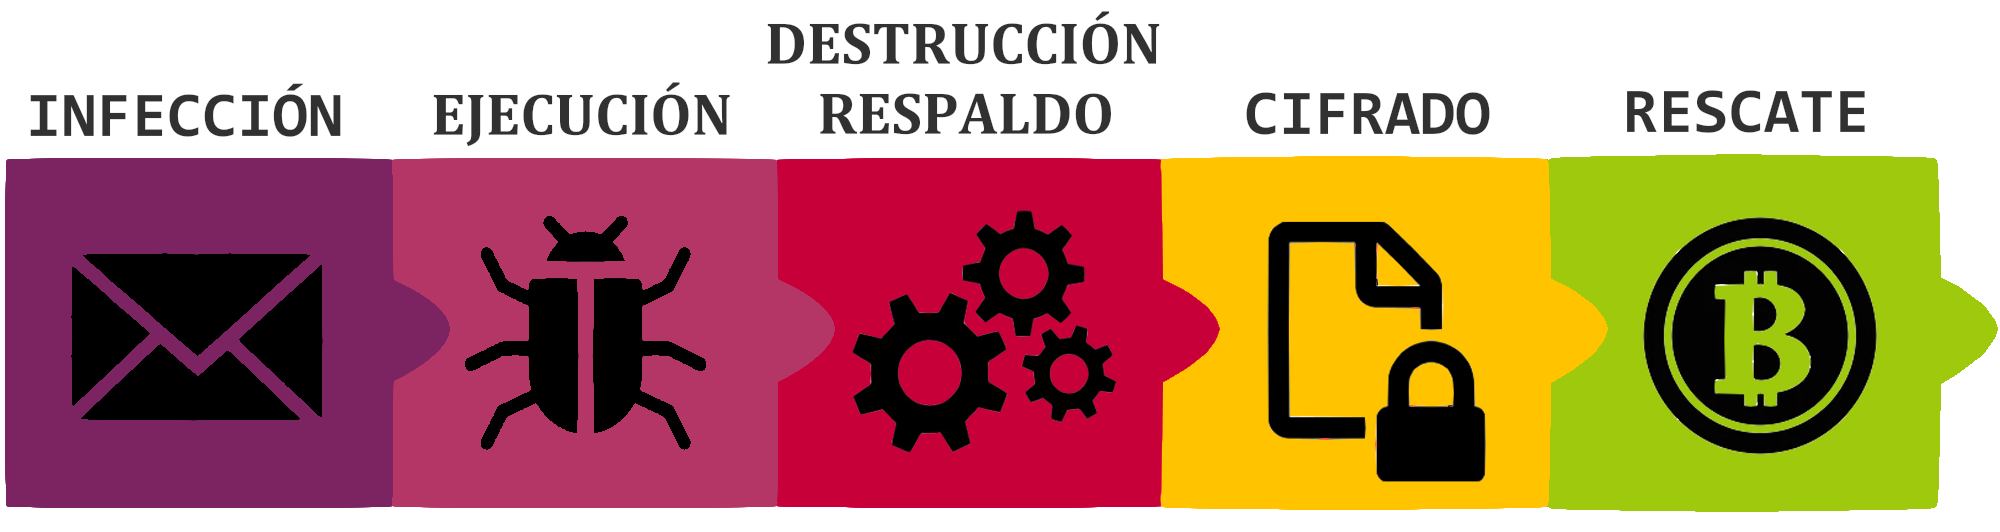
\includegraphics{images/etapas-ataque.png}}}
\end{center}
\caption{Patrón de ataque de un ransomware.}
\label{fig:imstages}
\end{figure}



\subsection{Métodos de Cifrado}
\noindent El ransomware moderno, como WannaCry, Petya o Locky, utiliza esquemas de cifrado híbrido, dificultando aún más la labor de recuperar la información cifrada en el ataque \cite{ransEncr}. A continuación se exponen los métodos de cifrado de archivos más importantes \cite{cypher}:

\begin{enumerate}
    \item \textbf{Cifrado simétrico}: También denominado cifrado de clave secreta. El texto plano se cifra y se descifra con la misma clave. La seguridad del cifrado no depende del algoritmo, si no de la privacidad de la clave. Permite que el ransomware cifre los datos a gran velocidad, y posteriormente almacena en disco las claves para almacenar cada archivo. Existen dos tipos de algoritmos simétricos:
    \begin{itemize}
        \item \textbf{Cifrado de bloque}: Procesa la entrada del texto en bloques de tamaño fijo y produce un texto cifrado de igual tamaño. Los más importantes son \gls{DES}, \gls{3DES}, vistos en la Figura \ref{fig:imdes} y \gls{AES}.
        
        \begin{figure}[htb!]
        \begin{center}
        \subfigure[Cifrado]{
            {\scalebox{.93}{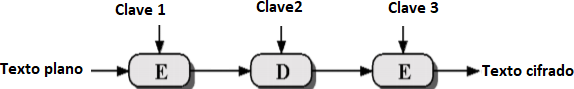
\includegraphics{images/3des_1.png}}}
            \label{fig:des1}}
        \subfigure[Descifrado]{
            {\scalebox{.93}{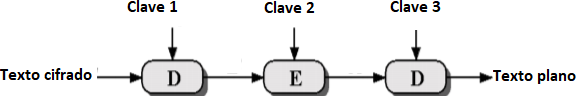
\includegraphics{images/3des_2.png}}}
            \label{fig:des2}}
        \caption{El algoritmo 3DES aplica 3 veces el algoritmo DES con claves distintas}
        \label{fig:imdes}
        \end{center}
        \end{figure}
        
        \item \textbf{Cifrado de flujo}: Procesa elementos de entrada y produce un elemento de salida. El más importante es \gls{RC4}.
        
    \end{itemize}
    
    \item \textbf{Cifrado asimétrico}: También denominado cifrado de clave pública. Está basado en funciones matemáticas en lugar de usar operaciones binarias sobre patrones de bits, por lo tanto este cifrado es más lento. Usa dos claves distintas: una pública y otra privada. El ransomware utiliza la clave pública para cifrar los archivos, y la clave privada es enviada al servidor de mando y control para ser almacenada, por lo que se necesita una conexión a internet. Los algoritmos más utilizados son \gls{DSA}, \gls{RSA} y \gls{DH}. Se diferencian las siguientes aplicaciones:
    \begin{itemize}
        \item \textbf{Cifrado con clave pública}: El emisor cifra con la clave pública del receptor y el receptor descifra con la clave privada.
        \item \textbf{Intercambio de clave}: Dos partes cooperan para establecer una clave secreta compartida.
        \item \textbf{Firma digital}: técnica utilizada para asegurar la autenticación y la integridad de los datos.
        \item \textbf{Certificado digital}: Se utiliza para proporcionar autenticación de las partes y no repudio
    \end{itemize}
    
    \item \textbf{Cifrado híbrido}: Usa cifrado simétrico y asimétrico. No necesita conexión a internet en el cifrado, pero sí en el descifrado. El ransomware y el servidor de mando y control generan un par de claves. Se cifrará la clave privada del cliente utilizando la clave pública del servidor. Al finalizar, todas las claves serán cifradas con la clave pública del cliente. Un ejemplo es el algoritmo utilizado por Locky: \gls{RSA}-2048+\gls{AES}-128 \cite{ransEncr}.
\end{enumerate}

\section{Detección}\label{sec:2-8}
\noindent Las técnicas usadas por los software de antivirus para reconocer la presencia de ransomware en el equipo son las siguientes \cite{ransommasive}:
\begin{itemize}
    \item \textbf{Detección basada en firma digital}: Cuando la compañía del antivirus descubre el malware crea una firma única para el tipo en concreto, y actualiza la base de datos del antivirus para poder comparar y capturar cuando el malware intente acceder a dicho equipo. No puede detectar avanzados tipos de malware polimórficos o que utilizan técnicas de cifrado para evadir dicha detección. 
    \item \textbf{Análisis del comportamiento}: Esta técnica trata de identificar el malware mediante los cambios que produce en el sistema, como puede ser la eliminación de ficheros, el aumento de la entropía (para cifrar los ficheros), las conexiones a redes extrañas, etc. Para recopilar estos datos, una técnica es registrar las llamadas a las \gls{API}s, los recursos del sistema que se están utilizando, los archivos que abre cada proceso, e introducirlas en una solución de \gls{ML} que sea capaz de detectar si esa serie de llamadas pueda corresponder a la ejecución de un ransomware \cite{Arabo2020}. 
    \item \textbf{Detección heurística}: Se basa en reglas y algoritmos para analizar si el código es malicioso. Puede realizarse un análisis estático, mediante un estudio de los indicadores sin ejecución como anomalías estructurales del código, el desmontaje del programa o el estudio de los elementos de una secuencia dada (n-gramas). Análogamente, el análisis dinámico, realiza un estudio de los indicadores del código en ejecución mediante técnicas de \textit{sandboxing} o virtualización \cite{DUBE2012137}. 
    \item \textbf{Detección usando la nube}: El archivo sospechoso se envía a un antivirus en la infraestructura de la nube del vendedor, aprovechando la capacidad computacional de la plataforma para analizarla de manera más rápida y eficiente. 
\end{itemize}

Además de las técnicas usadas por los antivirus y debido a que un ransomware puede cifrar archivos en cuestión de minutos, es importante implementar una detección a tiempo real tanto en el ordenador del usuario como en servidores web. Para implementar esta detección es importante seguir estos pasos \cite{74}:
\begin{itemize}
\item \textbf{Implementar escáneres de vulnerabilidad}: Se necesita saber en todo momento la información del sistema y de sus archivos tanto en local como en la nube. 
\item \textbf{Detección de intrusiones}: El ransomware es difícil de detectar antes de que ataque, pero un buen sistema de detección de intrusiones puede ser lo suficientemente rápido como para frenarlo antes de que cifre algún archivo. Un sistema de detección de intrusiones puede detectar comportamientos característicos de un ataque de ransomware en sus etapas iniciales \cite{107}. Algunos ejemplos de estos comportamientos son: deshabilitar el cortafuegos o el software antivirus, iniciar escáneres de red no autorizados, enviar datos a través de un canal encubierto y actualizar la política de auditoría.
\item \textbf{Activar la monitorización de la integridad de archivos}: Una parte principal del malware, incluyendo el ransomware, es ejecutar procesos para obtener permisos que le permitan acceder a los archivos del sistema. Estos procesos no se ejecutan normalmente, por lo que la monitorización de la integridad de los archivos puede generar una alerta cada vez que los detecta. Esto no va a prevenir el inicio del cifrado de archivos, pero puede evitar futuros ataques y poder aislar y poner en cuarentena el sistema infectado \cite{108}.
\item \textbf{Implementar la automatización de la seguridad}: Una respuesta rápida es un factor crítico de éxito en cualquier tipo de emergencia. Las innovaciones en el sector de la automatización y gestión de la seguridad han mejorado significativamente la respuesta ante amenazas, asegurando el funcionamiento conjunto de varias herramientas de seguridad. Este enfoque puede proporcionar una desconexión inmediata de la red y el aislamiento de los sistemas cuando se detecten las actividades del ransomware \cite{109}.
\item \textbf{Gestionar y analizar los registros}: Los objetivos del atacante se encuentran en los registros del sistema, de las aplicaciones, de la actividad... Detectar el acceso a los registros es complicado debido a la gran cantidad de ellos, por lo que es necesario automatizar su gestión y análisis.
\item \textbf{Combinar inteligencia sobre amenazas con la monitorización del sistema}: Los desarrolladores de ransomware más experimentados están en constantemente evolucionando sus métodos y código. Los analistas de seguridad deben investigan cuidadosamente su desarrollo, innovación e infraestructura para desarrollar métodos de gestión pro-activos (por ejemplo, software para la correlación de eventos) y herramientas para detectar los últimos ataques de ransomware.
\end{itemize}

\section{Prevención}\label{sec:2-9}

\noindent Se diferencian las estrategias de defensa que siguen las empresas contra los ataques ransomware y las acciones que han de seguir los usuarios finales para no estar expuestos \cite{ransommasive}.

\subsection{Defensa Individualizada}
\noindent La seguridad del equipo del usuario final es clave para proteger la red entera de una organización, puesto que basta con infectar un equipo para que algunos tipos de ransomware puedan propagarse por la totalidad de ellos. Al contrario de lo que piensa mucha gente, no basta solo con instalar un antivirus, sino que hay que cumplir una serie de acciones para alcanzar un grado de seguridad superior \cite{ransommasive}:
\begin{itemize}
    \item \textbf{Mantener respaldo de los datos}: Si los datos cifrados estaban replicados de manera consistente en otro dispositivo o en la nube, se pueden recuperar sin problema sin tener que pagar ningún rescate.
    
    \item \textbf{Mantener el sistema operativo y las aplicaciones actualizadas}: Sirven para arreglar las vulnerabilidades detectadas. El sistema operativo debe estar configurado para actualizarse tan pronto como la actualización esté disponible. Esto permitirá que el sistema sea más seguro frente a las vulnerabilidades, los kits de \textit{exploit}, etc. 
    
    \item \textbf{Uso de la virtualización}: El uso de máquinas virtuales permite ejecutar programas, descargarlos de internet y visitar páginas web comprometidas debido a que se ejecuta en un entorno seguro aislado del sistema operativo raíz. Aun así se debe mantener la precaución de que no el ransomware no se propague por la red en la que se encontraba la máquina virtual.
    
    \item \textbf{Bloquear la redirección web}: Esto evita páginas web no deseadas y enlaces maliciosos. Los navegadores actuales permiten esta configuración. También es buena práctica añadir extensiones al navegador para bloquear anuncios y \textit{pop ups} maliciosos, incluso algunas como \href{https://noscript.net/}{\textcolor{blue}{NoScript}}, que únicamente permite que se ejecuten los \textit{plugins} en los sitios web establecidos por el usuario.
    
    \item \textbf{Deshabilitar macros de Microsoft Office}: Como se ha explicado en la Sección \ref{item:macros} esta característica puede ser explotada para introducir ransomware en el equipo víctima. Además, es aconsejable abrir los archivos de Office recibidos vía correo electrónico en otra plataforma como Google Docs.
    
    \item \textbf{Dipositivos \gls{USB}}: Está totalmente desaconsejado conectar dispositivos desconocidos, poco fiables o encontrados en el sistema, puesto que puede contener ransomware que se instale al conectarlo. En algún caso, se debe configurar el antivirus para que escanee la unidad antes de montarla.
    
    \item \textbf{Modificar la extensión de los archivos importantes}: Algunos tipos de ransomware como WannaCry, cifran los ficheros basándose en una búsqueda por la extensión.
    
    \item \textbf{Remote Desktop Protocol}: Este protocolo permite el acceso remoto a un ordenador, de manera que si un atacante se conecta, podría infectar el equipo. Para restringir el acceso se recomienda utilizar una contraseña consistente, utilizar sesiones \gls{VPN} fiables y asegurarse de permitir conexiones autenticadas a nivel de red (\gls{NLA}).
\end{itemize}

\subsection{Estrategias Empresariales}
\noindent De manera complementaria a las medidas de seguridad que deben tomar los usuarios finales vistas en el apartado anterior, las organizaciones, empresas y gobiernos siguen una serie de estrategias de prevención en contra del auge de los ataques ransomware \cite{ransommasive}. 

\begin{itemize}
    \item \textbf{Seguridad física}: La seguridad de los equipos digitales (servidores, almacenamiento del respaldo, ordenadores, dispositivos de red) es tan importante como la de los datos almacenados en ellos. Para asegurarlos, se deben cumplir una serie de reglas como la restricción del acceso con medidas biométricas, monitorizar y restringir los espacios, no dejar equipos desatendidos, desconectar de la red sistemas sin utilizar, etc. 
    \item \textbf{Segmentación de red}: Es una medida para luchar contra el ransomware que limita la posibilidad del atacante de acceder al segmento donde se encuentra la información sensible. En la Figura \ref{fig:im11} de pueden ver las ventajas de esta segmentación.
    \begin{figure}[htb]
    \begin{center}
    {\scalebox{.9}{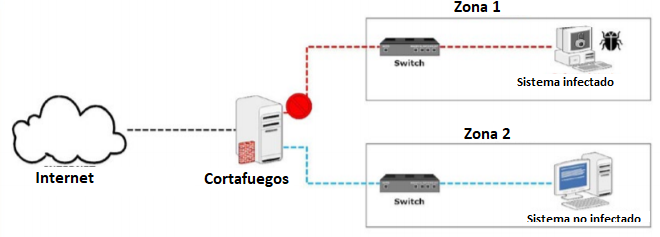
\includegraphics{images/segmentacion.png}}}
    \end{center}
    \caption{Ventajas de la segmentación de la red}
    \label{fig:im11}
    \end{figure}
    \item \textbf{Cortafuegos modernos}: Cualquier plan de seguridad comienza instalando un cortafuegos en el perímetro de la red, limitando las conexiones y permitiendo solo las permitidas. Los de nueva generación añaden otras herramientas de seguridad como antivirus, antimalware y el soporte para las redes privadas virtuales (\gls{VPN}).
    \item \textbf{Seguridad de correo electrónico}: Puesto que es el acceso más utilizado por el ransomware se deben desarrollar sistemas de filtrado avanzado de \textit{spam} mediante filtrado de \gls{IP} y contenido y deshabilitar el código \gls{HTML} en los e-mails recibidos por texto plano.
    \item \textbf{Formación de los trabajadores}: Para la creación de un entorno seguro, los trabajadores de la organización deben ser conscientes del riesgo existente y poner a su disposición la formación necesaria y los hábitos que deben seguir, como utilizar contraseñas seguras, no acceder a enlaces ni descargas de e-mails desconocidos, no conectar dispositivos extraños, etc \cite{TOPAYORNOT}.
    \item \textbf{Honeypots}: Se tratan de señuelos con información falsa que se anuncian online como objetivos de valor para cibercriminales y que permiten la detección de los ataques. En la Figura \ref{fig:im10} se aprecia el funcionamiento de honeypot.
    \begin{figure}[htb]
        \begin{center}
        {\scalebox{.9}{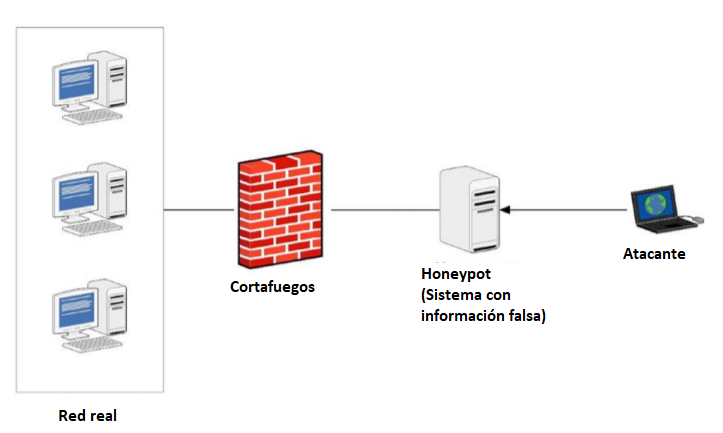
\includegraphics{images/honeypot.png}}}
        \end{center}
        \caption{Funcionamiento de honeypot}
        \label{fig:im10}
    \end{figure}
\end{itemize}


\section{Período Post-ataque}\label{sec:2-10}
\noindent Una vez el sistema ha sido infectado, se plantea una cuestión fundamental: ¿se debe pagar el rescate para recuperar el equipo infectado? La respuesta de los expertos es clara: no. Por un lado, te convertirías en un mayor objetivo, puesto que esta información es compartida entre atacantes, y conociendo que ya has pagado una vez, podrás hacerlo en otras ocasiones. Además, aunque cada vez más los criminales están cumpliendo con devolver los archivos (un ejemplo de ello es Cryptolocker, que permite descifrar 5 archivos elegidos de manera gratuita) debido a que creando esta confianza, más gente pagará por el rescate,  no se puede establecer confianza en los cibercriminales y en que el equipo sea descifrado. Por último, pagar el rescate provoca que los cibercriminales tengan más motivos para seguir con su labor \cite{TOPAYORNOT}. 

Si se ha decidido no pagar el rescate por los datos cifrados todavía se puede albergar alguna esperanza. Se debe realizar una valoración para conocer si se pueden recuperar los archivos cifrados siguiendo unos pasos \cite{CcnCert}:
\begin{enumerate}
    \item \textbf{Respaldo}: Si se dispone de una copia de seguridad, se procede a la desinfección del sistema y a la restauración de la copia de seguridad.
    \item \textbf{Herramientas de descifrado}: Aunque existen pocas variantes de ransomware que se puedan descifrar, por la intervención del \gls{CyC} y se han obtenido las claves, o porque existen vulnerabilidades en el código malicioso, hay disponibles herramientas públicas para descifrar archivos atacados por ransomware concreto, que se listan en la Tabla \ref{tab:recu}.
    

    \item \textbf{Shadow Volume Copy}: Si el ransomware no ha deshabilitado esta función como se ha expuesto previamente, se podrían restaurar los datos que Windows duplica automáticamente estableciendo una copia de seguridad.
    \item \textbf{Software forense}: En algunos casos es factible la recuperación de algunos ficheros originales mediante programas de análisis forense.
\end{enumerate}



    \begin{table}[htb!]
    \centering
    \scriptsize %para hacer la tabla mas pequeña
    \caption{Herramientas para la recuperación de datos}
    \begin{tabular}{|c|p{11.9cm}|}
        \hline
        \rowcolor[HTML]{C0C0C0}
        \textbf{Ransomware} &
        \multicolumn{1}{c|}{\cellcolor[HTML]{C0C0C0}{\textbf{Recuperación de ficheros}}} \\ \hline
        \textbf{Cerber}  &   En las versiones 1 y 2 herramienta Check Point. Versiones posteriores mediante 
        copia de seguridad \\ \hline
        \textbf{Crytolocker} & Comprobar en la web \url{http://www.decryptcryptolocker.com/} por si existe solución para su caso \\ \hline
        \textbf{Locky} & Comprobar mediante la herramienta Autolocky \\ \hline
        \textbf{Petya} & Primera versión: herramienta Bleepingcomputer. Segunda versión: publicada la clave privada. \\ \hline
        \textbf{Wannacry} & Solo mediante copia de seguridad. \\ \hline
        \textbf{Crysis}  & Algunas variantes mediante RakhniDecryptor \\ \hline
        \textbf{NotPetya}    & Solo mediante copia de seguridad \\ \hline
        \textbf{Cryptowall}  & Tercera versión mediante herramientas de recuperación de ficheros. Las demás versiones mediante copia de seguridad. \\ \hline
        \textbf{Cryptodefense} & Herramienta Emsisoft. \\ \hline 
    \end{tabular}
    \label{tab:recu}
    \end{table} 

\chapter{Análisis e Identificación de Malware}\label{Capitulo3}

\noindent En este capítulo se aborda el análisis de malware, en qué consiste, su importancia y los tres tipos de análisis que existen: el estático \ref{sec:aestatico}, el dinámico \ref{sec:adinamico} y el híbrido \ref{sec:ahibrido} . El capítulo termina explicando el aprendizaje automático aplicado al análisis de malware \ref{sec:mlaplicado} y los algoritmos más usados para el desarrollo de modelos que detecten automáticamente las amenazas. 



\section{Introducción}

\noindent El análisis de malware es el estudio del comportamiento del malware, y su objetivo es comprender el funcionamiento del malware, sus capacidades, cómo detectarlo, contenerlo y/o eliminarlo \cite{113}. Esto implica analizar el programa sospechoso en un entorno seguro para identificar sus características y así poder construir mejores defensas para defender la red de una empresa. Además, analizar malware sirve para encontrar vulnerabilidades en nuestros sistemas, nuevos métodos de infección y la evolución de los atacantes y sus propósitos \cite{LMA2018}.
Las razones por las que es importante realizar un análisis de malware son \cite{75}:
\begin{itemize}
\item Determinar la naturaleza y finalidad del malware. Es importante saber si el malware es un ransomware, un \textit{spyware} \cite{114}, un \textit{rootkit} \cite{115}, un \gls{RAT} \cite{116}, etc.
\item Entender cómo se vio comprometido el sistema y el impacto que tuvo el malware sobe él \cite{118}.
\item Encontrar los indicadores de red del malware mediante la monitorización de la red. Estos indicadores se utilizan para detectar infecciones parecidas. Por ejemplo, si durante el análisis se concluye que un malware contacta con una dirección \gls{IP} en particular, se puede monitorizar el tráfico de la red para identificar todos los equipos que contactan con esa dirección.
\item Extraer conclusiones como claves de registro y nombres de archivo basándonos en el equipo. También se utilizan para detectar una infección parecida en otro equipo. Por ejemplo, si un malware crea una clave de registro, se puede utilizar esa misma clave como indicador para identificar todos los equipos que tienen la misma clave de registro.
\item Determinar el motivo del atacante, su intención y su identidad si es posible para poder clasificar el malware correctamente. 
\end{itemize}

Para comprender el funcionamiento y las características del malware y evaluar su impacto en los sistemas que infecta, se utilizan tres tipos de análisis: estático, dinámico e híbrido. 


%Las principales metodologías de análisis de malware son el análisis estático (no ejecuta el malware) y el análisis dinámico (observa el comportamiento del malware mientras actúa).



\section{Análisis Estático}
\label{sec:aestatico}

\noindent El análisis estático de una muestra de malware consiste en analizar un binario en busca de signos de intenciones maliciosas sin tener que ejecutarlo \cite{111}, es decir, poder determinar si se trata de una muestra maliciosa antes de que comience a actuar, incluso es posible encontrar más información acerca del tipo y familia de malware y el comportamiento que tendrá \cite{Mohanta2020}. Es más fácil de realizar y permite extraer los metadatos asociados con el programa sospechoso.
Este tipo de análisis se puede interpretar como una ``disección'' del binario sin el riesgo de que el malware actúe en nuestro equipo \cite{EPN2014}.

A la hora de realizar análisis estático de una muestra, se utiliza principalmente un desensamblador para realizar la “disección” anteriormente mencionada y decodificar el código máquina del malware \cite{SIM2020}.

Puede que el análisis estático no revele toda la información necesaria, pero puede proporcionar información interesante que ayude a determinar el enfoque de los análisis posteriores. Para determinar si un archivo es malicioso, se usan indicadores técnicos denominados \gls{IoC} como nombres de archivo, direcciones \gls{IP}, dominios y datos en el encabezado del archivo \cite{90}, y herramientas como analizadores de red para observar el malware sin ejecutarlo para recopilar información sobre cómo funciona \cite{113}. 


\subsection{Técnicas}

\noindent La elección de la técnica para revelar información de un archivo potencialmente malicioso depende del objetivo y del contexto que rodea al archivo sospechoso \cite{89}. Algunas de las técnicas o fases de análisis estático son:

\begin{itemize}
    \item \textbf{Determinar el tipo de fichero y arquitectura}: La extensión del binario ayuda a averiguar cual es la máquina objetivo del malware (Windows, MacOS, etc.) y la arquitectura del mismo. Por ejemplo, si el tipo del archivo es \gls{PE}, que es el formato de archivo para los ejecutables de Windows (.exe, .dll, .sys, .drv, .com, .ocx, etc) \cite{96}, entonces se puede deducir por la extensión del archivo que el malware está diseñado para atacar el sistema operativo Windows.
    Aun así, esto no es del todo fiable ya que los atacantes utilizan diferentes trucos para ocultar el archivo, modificar la extensión real del fichero y cambiar su apariencia con el fin de engañar a los usuarios para que lo ejecuten.
    Para encontrar la extensión real de un fichero en Windows, es posible fijarse en la firma del mismo (\textit{file signature}). Una firma de archivo es una secuencia única de bytes que se escribe en su encabezado \cite{97}. los primeros bits indicarán si se trata de algún tipo de ejecutable (\gls{PE} files). Esto se puede determinar utilizando métodos manuales o herramientas específicas \cite{LMA2018}. 
    También es posible determinar si se está falseando la extensión o se trata de un archivo sospechoso prestando atención a sus propiedades (información o detalles de la versión, copyright de la aplicación, etc.) o con una aplicación específica, como CFF Explorer, para observar si la miniatura del archivo ha sido modificada para simular ser un fichero legítimo \cite{Mohanta2020}.

    \item \textbf{Huellas digital del malware}: Esta técnica consiste en la generación del \textit{hash} criptográfico para los binarios basándose en el contenido del fichero \cite{LMA2018}. Los algoritmos más comunes son MD5, SHA1 y SHA256 y a la hora de realizar un análisis es bueno generar los tres tipos de \textit{hashes} para la misma muestra. El motivo de generar el hash para una muestra es que podemos compartir esta información con plataformas de análisis u otros usuarios para identificar el malware sin tener que compartir el mismo, evitando infectar un equipo ajeno o transmitir información personal del usuario \cite{Mohanta2020}.La generación de estos valores \textit{hash} se realiza mediante la ejecución los comandos \textit{md5sum}, \textit{sha256sum} y \textit{sha1sum} en Linux o mediante el uso del módulo \textit{hashlib} en Python.


    \item \textbf{Inspección de la información del encabezado \gls{PE}}: La cabecera de un archivo, además de contener su tipo, incluye información sobre dónde se debe cargar el ejecutable en la memoria, la dirección donde comienza la ejecución, la lista de bibliotecas y funciones en las que se basa la aplicación y los recursos utilizados \cite{86}. Para realizar tales interacciones, el malware depende de las funciones del sistema operativo. Windows exporta estas funciones llamadas \gls{API} en archivos \gls{DLL} (archivos pertenecientes a bibliotecas de enlaces dinámicos) \cite{103}. Los ejecutables importan y llaman a estas funciones normalmente desde varios archivos \gls{DLL} que proporcionan diferentes funcionalidades. La inspección de los archivos \gls{DLL} en las que se basa un malware y las funciones \gls{API} que importa pueden dar una idea sobre la funcionalidad y capacidad del malware. Toda esta información de las importaciones se almacena en tablas en el encabezado \gls{PE} \cite{75}.

    \item \textbf{Escaneo del virus con un programa específico como un antivirus}: Realizar esta acción ayuda a saber más acerca de la posible muestra maliciosa y mejorar nuestro análisis \cite{LMA2018}. Para ello, se suele utilizar algún antivirus específico que instalado en el equipo o en páginas web como VirusTotal o Jotti Virus Scan, que ofrecen un servicio de escaneo de malware con varias fuentes con el fin de determinar la peligrosidad de una muestra y almacenan toda la información obtenida a la cual se puede acceder y se comparte con empresas u organizaciones interesadas. Además, existen otras plataformas web como “file2scan” o “scan4you” las cuales son de pago y no comparten la información con nadie, siendo el escaneo anónimo, lo que permite a cibercriminales comprobar la peligrosidad de sus archivos maliciosos \cite{EPN2014} \cite{LMA2018}. El riesgo que existe en esta técnica es que el escaneo no detecte el fin malicioso de la muestra, pero aún así, siga tratándose de un malware.
    
    \item \textbf{Detectar protección o empaquetadores}: Los creadores de malware en su mayoría buscan ocultar el contenido y funcionamiento del malware para que en el análisis del mismo sea difícil o imposible encontrar esta información. Para realizar esto, se utilizan programas específicos conocidos como empaquetadores o \textit{packers} o \textit{cryptors} \cite{EPN2014}. Los empaquetadores o packers ocultan el ejecutable en un nuevo archivo que cuando se activa, “descomprime” el binario original para realizar el ataque. El \textit{cryptor} es parecido, pero utiliza cifrado en lugar de compresión \cite{LMA2018}. Para detectar este tipo de empaquetado o cifrado, se pueden utilizar herramientas como Exeinfo PE,  PEiD o RDG Packer Detector.
    
    \item \textbf{Extracción de cadenas, funciones y metadatos asociados con el binario}: Las cadenas son secuencias de caracteres en \gls{ASCII} y \textit{Unicode} contenidas en un archivo \cite{101}. La extracción de estas cadenas  puede dar pistas sobre la funcionalidad del programa, ya que contienen referencias a nombres de archivo, varias \gls{URL}, nombres de dominio, direcciones \gls{IP}, comandos de ataque, claves de registro, etc. Aunque las cadenas no dan una imagen clara del propósito y la capacidad de un malware, puede ayudar a encontrar información sobre la acción del fichero malicioso o sobre el atacante, como por ejemplo el tipo de malware, direcciones \gls{IP}, comandos de ataque, claves, objetivos del malware, etc. \cite{LMA2018}. Para extraer estas cadenas, existe un comando en Linux llamado \textit{strings}, pero esto sólo es posible si la información no ha sido ocultada mediante \textit{packers} o \textit{cryptors} o si estos han empleado una protección vulnerable. Para estos casos se puede usar la herramienta \textit{pestudio} para extraer cadenas de un binario sospechoso o a \gls{FLOSS} para detectar y extraer información oculta \cite{102}.
    
    \item \textbf{Clasificación de las muestras}: Con el fin de conocer características específicas de un malware o su pertenencia, se compara el binario con otras muestras analizadas previamente o almacenadas en un repositorio que puede ser privado o público. El \textit{hash} criptográfico visto anteriormente es una gran técnica para detectar muestras idénticas, pero no ayuda a identificar muestras similares ya que a menudo los delincuentes cambian ciertos parámetros del malware que modifican el \textit{hash} por completo y dificulta esta tarea. Para poder clasificar las muestras de malware se pueden utilizar técnicas como \textit{Fuzzy Hashing} (mediante la herramienta \textit{ssdeep}) \cite{104}, \textit{Import Hash} (que mira las funciones \gls{API} llamadas por los dos archivos)  \cite{105} o YARA (una herramienta para crear reglas que consisten en expresiones booleanas y cadenas basadas en patrones de información del binario para poder identificarlo cuya complejidad puede ser muy alta) \cite{YARADOC} \cite{77}. 
\end{itemize}

En la Figura \ref{fig:staticFlow} se muestra el diagrama de flujo del proceso de un análisis estático, mencionando todas las técnicas explicadas anteriormente.

\begin{figure}[h!]
\begin{center}
{\scalebox{.3}{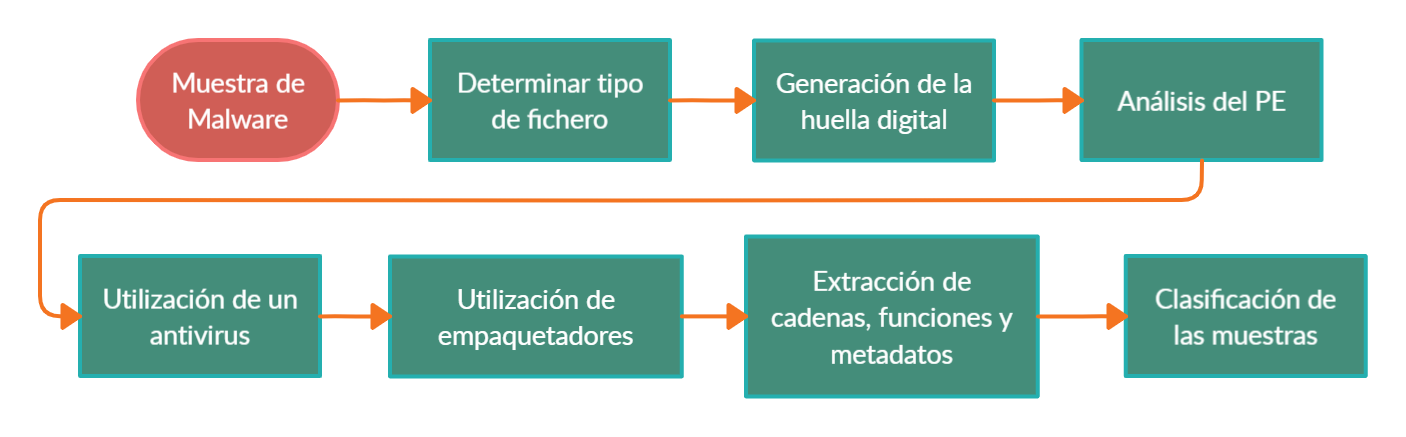
\includegraphics{images/static-flow.png}}}
\end{center}
\caption{Diagrama de flujo de un análisis estático.}
\label{fig:staticFlow}
\end{figure}

El problema del análisis estático es que, al no ejecutar el código, un malware más sofisticado puede incluir comportamientos maliciosos en tiempo de ejecución que pueden pasar desapercibidos. Por ejemplo, si descarga un archivo malicioso basado en una cadena dinámica, el análisis estático no lo detectará \cite{117}. Es por esto por lo que las empresas recurren al análisis dinámico para una comprensión más completa del comportamiento del malware.

\subsection{Herramientas}

\noindent Existen diferentes herramientas de análisis estático según la técnica que apliquen, algunas de las más conocidas y usadas se muestran en la Tabla \ref{tab:toolsEst}.

\begin{table}[htb!]
\centering
\scriptsize %para hacer la tabla mas pequeña
\caption{Herramientas de análisis estático}
\begin{tabular}{|l|p{12cm}|}
\hline
\rowcolor[HTML]{C0C0C0}
\multicolumn{1}{|c|}{\cellcolor[HTML]{C0C0C0}{\textbf{Herramienta}}} & \multicolumn{1}{c|}{\cellcolor[HTML]{C0C0C0}{\color[HTML]{000000} \textbf{Descripción}}}\\ \hline

    \textbf{WinMD5Free}& Una herramienta gratuita con interfaz gráfica para calcular el \textit{hash} de un fichero utilizando el algoritmo \gls{MD5} para comprobar comparando el \textit{hash} generado si el fichero ha sido alterado en algún momento \cite{EPN2014}.\\ \hline
    
    \textbf{CFF Explorer}& Un conjunto de herramientas gratuitas destinado a la monitorización de procesos y la edición de ficheros \gls{PE} que permite la modificación de campos especiales, incluye desensamblador y gestión de firmas entre otras muchas funcionalidades \cite{EPN2014}.\\ \hline

    \textbf{Ollydbg}& Un simple depurador sólo para sistemas Windows de 32 bits enfocado principalmente al análisis de código binario. Las diferentes características de este programa permiten usar \textit{breakpoints} y cambiar instrucciones y condiciones en el ejecutable, además, es libre y no necesita instalación. Destaca también por tener una gran variedad de \textit{plugins} \cite{Vokorokos2017}.\\ \hline
    
    \textbf{Ghidra}&Herramienta desarrollada en Java analiza tanto ficheros \gls{PE} como \gls{ELF} y puede utilizarse en Windows, Linux y MacOS. Se trata de un proyecto desarrollado por la \gls{NSA} de Estados Unidos que, además de desensamblar binarios, contiene un decompilador para sacar un pseudocódigo en lenguaje C del fichero analizado \cite{SIM2020}.\\ \hline
    
    \textbf{IDA Pro}& Es un proyecto de Hex-Rays utilizado para ingeniería inversa del cual se puede obtener una versión básica con pocas funcionalidades gratuitamente. Básicamente, \gls{IDA} Pro es un sofisticado desensamblador con múltiples funcionalidades en su versión completa que busca hacer el código complejo más legible para el usuario \cite{IDA2011}.\\ \hline
    
     \textbf{Radare2}& Un proyecto libre el cual se puede obtener de un repositorio en GitHub y está basado en un conjunto de comandos que se pueden usar juntos o aislados. Cuenta con diferentes programas como rabin2, rasm2, rahash2… siendo el principal de todos radare2, que permite “diseccionar” un binario, analizar los datos, desensamblar el código, etc. Además, admite diferentes lenguajes, entre ellos Python, JavaScript o Perl \cite{RAD2ORG}. \\ \hline
    
    \textbf{PEiD}& Una de las herramientas más usada en todo el mundo para identificar \textit{packers} ya que es la que mejores resultados ha proporcionado. 
    Una de las claves de su éxito es que contiene un alto número de firmas de empaquetadores para identificar a estos. Además, es gratuita \cite{Kancherla2015}.\\ \hline
    
    \textbf{PEStudio}& Una sencilla aplicación libre usada para estudiar cualquier tipo de ejecutable extrayendo cadenas y firmas. Los resultados son similares a los que ofrece VirusTotal, lo que permite complementar la herramienta \cite{Amiruddin2020}.\\ \hline
\end{tabular}
\label{tab:toolsEst}
\end{table}

\subsection{Limitaciones}

\noindent Este tipo de análisis muchas veces no sirve para encontrar una resolución clara y es necesario cambiar de técnica si se quiere llegar a algún tipo de resultado. En definitiva el análisis estático sirve para encontrar información sobre la muestra y que esta ayude en una siguiente fase \cite{Mohanta2020}, además, este análisis puede ser muy complicado debido a que el código ensamblador sea ilegible, ya que algunas funciones las codifican y para poder leerlo sea necesario ejecutar el binario, por lo que ya se hablaría de análisis dinámico \cite{SIM2020}.

\section{Análisis Dinámico} \label{sec:adinamico}

\noindent El análisis dinámico de una muestra se realiza mientras que esta está siendo ejecutada y es más importante que nunca hacerlo en un entorno controlado montando un laboratorio de análisis \cite{111}.  Esta técnica de ejecutar el programa malicioso en un entorno seguro se conoce como \textit{sandboxing} \cite{122}, o aislamiento de procesos en español.  En este tipo de análisis se presta atención a las llamadas a \gls{API}, el tráfico de red o la actividad en procesos, en archivos o en el registro del sistema \cite{Gandotra2014}.
Para realizar el análisis dinámico se pueden utilizar tanto herramientas instaladas en un equipo como plataformas web que ahorran el trabajo de montar un laboratorio de análisis seguro. Normalmente, este análisis se realiza cuando el análisis estático ha llegado a un final ya sea porque es imposible analizarlo o porque los resultados no son satisfactorios.

El malware interactúa con el sistema de varias formas cuando es ejecutado, creando claves de registro y valores para su persistencia, descargando archivos, creando nuevos o comunicándose con un servidor \gls{CyC} \cite{123}. La monitorización de estas interacciones con el sistema y la red ayudará a comprender el propósito y la naturaleza del malware. 

%(la construcción del laboratorio destinado a este trabajo se detalla en el anexo \ref{anexo-a}).
\subsection{Técnicas de Análisis}

\noindent Al hablar de las técnicas de análisis dinámico, es preciso centrarse principalmente en la monitorización, sin dejar de prestar a atención al resto. 
Existen diferentes técnicas utilizadas en el análisis dinámico de malware; sin embargo, para conseguir los mejores resultados, será necesario combinarlas:

\begin{itemize}
    \item \textbf{Sandboxing}: \textit{Sandboxing} es una técnica que consiste en aislar la ejecución de un programa no fiable o malicioso llevándola a un entorno seguro que no comprometa el sistema, de forma que sea posible analizar las actividades del malware sin preocupación por los cambios que realice el proceso maligno. Existen múltiples herramientas que utilicen \textit{sandboxing} y permitan construir un laboratorio de análisis de malware, entre ellas, Buster Sandbox Analyzer, Zero Wine, Malheur o Cuckoo Sandbox. Normalmente estas herramientas simulan servicios de red para que el malware actúe con normalidad. Utilizar \textit{sandboxing} también tiene inconvenientes, por ejemplo, si el malware necesita un comando de activación o este actúa pasado un tiempo superior a la duración del análisis este no llegará a activarse y por lo tanto el análisis será fallido. Además, muchos malwares pueden detectar que se encuentran en una máquina virtual y debido a ello interrumpen su ejecución \cite{PMA2012}.
    \item \textbf{Creación de instantáneas}: Cuando para el análisis se cuente con un laboratorio seguro, las muestras serán ejecutadas en máquinas virtuales con las herramientas de análisis que se vayan a utilizar instaladas en ellas. Al ejecutar una muestra, esta puede realizar cambios en el sistema de la máquina virtual, dejar trazas o mantener el sistema infectado después de haber analizado el malware. En ese caso, si se reutiliza el entorno para analizar una nueva muestra, las acciones de análisis previos podrían interferir en el nuevo análisis. Para solucionar esto, se guarda el estado de la máquina virtual puesta a punto para su primer análisis mediante instantáneas (\textit{snapshots}) de forma que, tras analizar una muestra y obtener los resultados, se retroceda al estado inicial de la máquina para garantizar que ninguna ejecución de malware anterior interfiere en el análisis \cite{Mohanta2020}.
    \item \textbf{Monitorización}: Un malware puede interactuar tanto con el sistema como con la red, descargando algún componente malicioso, modificando el sistema de ficheros (crear nuevos archivos, borrar otros, etc.)  hacerse con el control del equipo  o comunicándose con un servidor \gls{CyC} entre otras cosas \cite{123}. Para estudiar el comportamiento del malware, se recurre a la monitorización de procesos, del sistema de ficheros, de registros y de red \cite{LMA2018}. Existen tipos de malware, como es el caso del ransomware, cuyo comportamiento es muy explícito y se puede notar a simple vista y otros que, si no se recurre a la monitorización, pueden pasar fácilmente por alto \cite{Mohanta2020}. 
    Los diferentes tipos de monitorización que se podrán realizar durante el análisis dinámico son\cite{75}:
\begin{itemize}
\item \textbf{Monitorización de procesos, del registro y del sistema de archivos}: Implica monitorizar las actividades de los procesos y examinar sus propiedades, ver si interactúan con el sistema de archivos y si acceden o modifican claves de registro durante la ejecución del malware. Process Hacker \cite{93} es una herramienta de código abierto para examinar los procesos que se ejecutan en el sistema e inspeccionar sus atributos. También se puede utilizar para explorar servicios, conexiones de red, actividad del disco, etc. Una vez que se ejecuta la muestra de malware, esta herramienta puede ayudar identificar dicha muestra y examinar sus atributos o detener la ejecución. Process Monitor \cite{94} es otra herramienta enfocada en la supervisión que muestra la interacción en tiempo real de los procesos con el sistema de archivos, el registro y la actividad de procesos y subprocesos. Para solo centrarse en las actividades resultantes de la actividad del malware, hay opciones de filtrado que permiten filtrar por atributos específicos. Pero esto puede resultar muy tedioso, por lo que existe un programa en Python llamado Noriben \cite{95} que viene con filtros predefinidos. 
\item \textbf{Monitorización de la red}: Es el estudio del tráfico de la red durante la ejecución de malware en el sistema, necesario para encontrar el canal de comunicación utilizado dicho malware y para determinar los indicadores basados en la red. Como ya sabemos, la mayoría del malware al ejecutarse se comunica con un servidor \gls{CyC}. Para realizar un análisis completo, hay que emular este servidor para proporcionar al malware todos los servicios requeridos para que pueda continuar con su funcionamiento. INetSim \cite{91} es un software gratuito basado en Linux para simular servicios de Internet, como un servidor ficticio, que es justo lo que necesitamos. INetSim puede registrar comunicaciones y también puede responder a solicitudes \gls{HTTP} o \gls{HTTPS} y devolver archivos. Por ejemplo, si el malware solicita un archivo ejecutable, INetSim se lo puede proporcionar. De esa manera se podrá saber qué hace el malware con el archivo después de descargarlo del servidor \gls{CyC}.
\end{itemize}
    
    \item \textbf{Simulación de una red}: Muchos malwares establecen conexión con un servidor externo en la red y si el entorno de análisis no permite conexión a Internet, estas muestras nunca mostrarán su comportamiento al completo. Para solucionar esto, se simula una red y así se obtiene información como \gls{DNS} o direcciones \gls{IP}. En muchas ocasiones, si se utiliza una herramienta de \textit{sandboxing}, se tiene la opción de simular una red \cite{PMA2012}.
    \item \textbf{Análisis de bibliotecas de vínculos dinámicos (\gls{DLL})}: Una \gls{DLL} es un módulo con código y datos que utilizan los distintos programas para realizar cierta función de la \gls{DLL}, ayudando a promover la reutilización de código y el uso eficaz de la memoria \cite{DLL2020}. Las funciones exportadas por los archivos \gls{DLL} se llaman \gls{API} (interfaces de programación de aplicaciones en español) \cite{75}.  Los sistemas operativos proporcionan a las aplicaciones las \gls{API} para que puedan realizar tareas comunes, como interactuar con el sistema de archivos, el registro del sistema, la red y la interfaz gráfica de usuario \cite{113}. Los últimos sistemas operativos de Windows proporcionan tanto una \gls{API} nativa (llamadas al sistema) como una \gls{API} de Windows \cite{119}. Muchas veces los autores de malware implementan el código como \gls{DLL}s ya que esto permite al atacante cargar la \gls{DLL} en cualquier proceso, proporcionando la persistencia del malware en el sistema y ocultando la actividad maliciosa \cite{LMA2018}. Analizar la interacción que realiza el malware mediante \gls{DLL}s es un factor muy importante en el análisis dinámico.
\end{itemize}

En la Figura \ref{fig:dinamFlow} se muestra el diagrama de flujo del proceso de un análisis dinámico, en el que se puede ver todo lo explicado anteriormente.

\begin{figure}[h!]
\begin{center}
{\scalebox{.35}{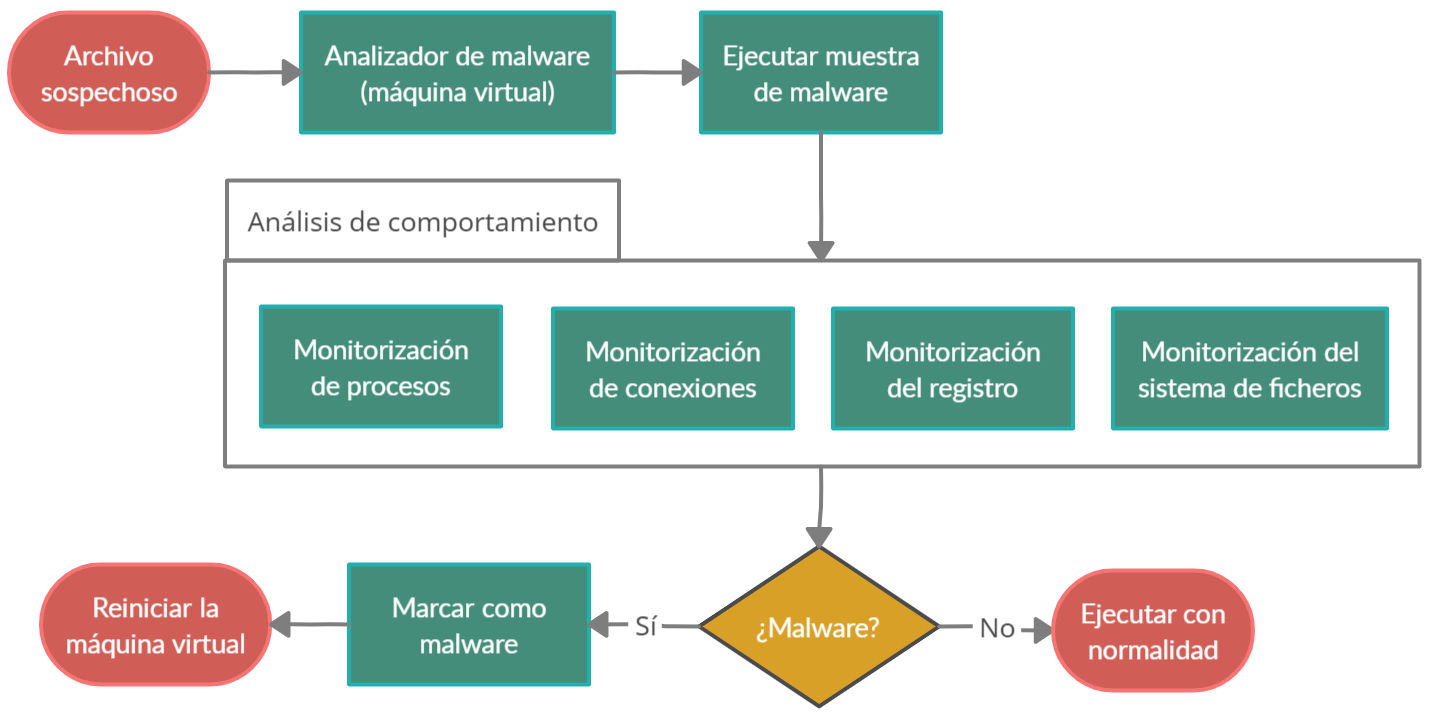
\includegraphics{images/dynamic-flow.png}}}
\end{center}
\caption{Diagrama de flujo de un análisis dinámico.}
\label{fig:dinamFlow}
\end{figure}

\subsection{Herramientas}

\noindent Cuando se habla de las herramientas de análisis dinámico, se puede diferenciar entre análisis dinámico automatizado y análisis dinámico manual. Por lo general, los programas o plataformas web basadas en \textit{sandboxing} pertenecen al análisis automatizado e incluyen monitorización, en cambio, las herramientas de análisis manual implican controlar la información que se quiere obtener de ella y analizarla después. En la Tabla \ref{tab:toolsDin} se muestran las herramientas más utilizadas en el análisis dinámico de malware que no hayan sido explicadas anteriormente.

\begin{table}[htb!]
\centering
\scriptsize %para hacer la tabla mas pequeña
\caption{Herramientas de análisis dinámico.}
\begin{tabular}{|l|p{11.5cm}|}
\hline
\rowcolor[HTML]{C0C0C0}
\multicolumn{1}{|c|}{\cellcolor[HTML]{C0C0C0}{\textbf{Herramienta}}} & \multicolumn{1}{c|}{\cellcolor[HTML]{C0C0C0}{\textbf{Descripción}}}\\ \hline
\textbf{Cuckoo Sandbox}&Herramienta de análisis automatizado de malware de código abierto en Windows, macOS, Linux y Android que utiliza la tecnología de sandboxing. Cuckoo Sandbox tiene un diseño modular, lo que permite personalizar cualquier aspecto del procesamiento del análisis de los resultados, de la generación de informes y del entorno de análisis.\\ \hline
\textbf{Regshot}& Programa que realiza dos instantáneas (una antes de ejecutar el malware y otra después) y las compara encontrando los valores modificados durante la actuación del código malicioso \cite{PMA2012}.\\ \hline
    \textbf{Wireshark}&Herramienta más usada en todo el mundo para analizar el tráfico de red con gran detalle. Soporta gran variedad de plataformas y protocolos y dispone de múltiples filtros, formatos y formas de exportar la información obtenida \cite{WRSKDOC} \cite{92}.\\ \hline
    \textbf{ApateDNS}&Herramienta gratuita que se puede utilizar para encontrar peticiones \gls{DNS} realizadas por un malware. Esto lo hace suplantando respuestas \gls{DNS} a una dirección IP específica escuchando en el puerto 53 \gls{UDP} en la máquina local \cite{PMA2012}.\\ \hline
    \textbf{APIMiner}& Herramienta que registra las llamadas a \gls{API} realizadas durante la actuación de una muestra. El resultado que ofrece es un registro de las llamadas a \gls{API} junto a sus argumentos ordenadas según el momento en el que fueron invocadas \cite{Mohanta2020}.\\ \hline
\end{tabular}
\label{tab:toolsDin}
\end{table}

\begin{comment}
\begin{itemize}
    \item \textbf{Cuckoo Sandbox}: Herramienta de análisis automatizado de malware de código abierto en Windows, macOS, Linux y Android que utiliza la tecnología de \textit{sandboxing}. Cuckoo Sandbox tiene un diseño modular, lo que permite personalizar cualquier aspecto del procesamiento del análisis de los resultados, de la generación de informes y del entorno de análisis.
    \item \textbf{Regshot}: Programa que realiza dos instantáneas (una antes de ejecutar el malware y otra después) y las compara encontrando los valores modificados durante la actuación del código malicioso \cite{PMA2012}.
    \item \textbf{Wireshark}: Herramienta más usada en todo el mundo para analizar el tráfico de red con gran detalle. Soporta gran variedad de plataformas y protocolos y dispone de múltiples filtros, formatos y formas de exportar la información obtenida \cite{WRSKDOC}.
    \item \textbf{ApateDNS}: Herramienta gratuita que se puede utilizar para encontrar peticiones \gls{DNS} realizadas por un malware. Esto lo hace suplantando respuestas \gls{DNS} a una dirección \gls{IP} específica escuchando en el puerto 53 \gls{UDP} en la máquina local \cite{PMA2012}.
    \item \textbf{APIMiner}: Herramienta que registra las llamadas a \gls{API} realizadas durante la actuación de una muestra. El resultado que ofrece es un registro de las llamadas a \gls{API} junto a sus argumentos ordenadas según el momento en el que fueron invocadas \cite{Mohanta2020}.
\end{itemize}
\end{comment}
\subsection{Limitaciones}

\noindent El análisis dinámico es más efectivo que el análisis estático descrito anteriormente y no requiere desensamblar el ejecutable. El punto negativo del análisis dinámico es que el consumo de recursos es mayor y lleva más tiempo, aumentando los problemas de escalabilidad. Por otro lado, a veces el malware está destinado a un cierto sistema o condiciones del mismo (tener un motor de búsqueda concreto, determinadas \gls{DLL}s, etc.), o quizá tenga protección contra máquinas virtuales, lo que podría provocar que no se pueda detectar su comportamiento malicioso en el laboratorio de análisis seguro que se haya montado \cite{Gandotra2014}. En definitiva, lo más efectivo viene a ser combinar tanto el análisis estático como el análisis dinámico para conseguir el mejor resultado posible. La Tabla \ref{tab:tabla2} se muestra de manera clara las diferencias fundamentales entre el análisis el estático y el dinámico, indicando los métodos de análisis que usan cada uno \cite{121}. 

\begin{table}[h!]
\centering
\scriptsize %para hacer la tabla mas pequeña
\caption{Diferencias entre análisis dinámico y estático.}
\begin{tabular}{|l|c|c|}
\hline
\rowcolor[HTML]{C0C0C0}
\multicolumn{1}{|c|}{\cellcolor[HTML]{C0C0C0}{\textbf{Métodos de análisis}}} & \multicolumn{1}{c|}{\cellcolor[HTML]{C0C0C0}{\textbf{Estático}}} & \multicolumn{1}{c|}{\cellcolor[HTML]{C0C0C0}{\textbf{Dinámico}}} \\ \hline
{\color[HTML]{000000} Extracción de cadenas} & {\color[HTML]{000000} Sí} & {\color[HTML]{000000} No} \\ \hline
{\color[HTML]{000000} Secuencias de bytes} & {\color[HTML]{000000} Sí} & {\color[HTML]{000000} No} \\ \hline
{\color[HTML]{000000} Códigos de operación} & {\color[HTML]{000000} Sí} & {\color[HTML]{000000} No} \\ \hline
{\color[HTML]{000000} Llamadas a las \gls{API}} & {\color[HTML]{000000} Sí} & {\color[HTML]{000000} Sí} \\ \hline
{\color[HTML]{000000} Sistema de ficheros} & {\color[HTML]{000000} No} & {\color[HTML]{000000} Sí} \\ \hline
{\color[HTML]{000000} Registros de \gls{CPU}} & {\color[HTML]{000000} Sí} & {\color[HTML]{000000} Sí} \\ \hline
{\color[HTML]{000000} Características del \gls{PE}} & {\color[HTML]{000000} Sí} & {\color[HTML]{000000} No} \\ \hline
{\color[HTML]{000000} Monitorización de la red} & {\color[HTML]{000000} No} & {\color[HTML]{000000} Sí} \\ \hline
{\color[HTML]{000000} Acceso a memoria} & {\color[HTML]{000000} No} & {\color[HTML]{000000} Sí} \\ \hline
{\color[HTML]{000000} Sandboxing} & {\color[HTML]{000000} No} & {\color[HTML]{000000} Sí} \\ \hline
{\color[HTML]{000000} Excepciones} & {\color[HTML]{000000} No} & {\color[HTML]{000000} Sí} \\ \hline
\end{tabular}
\label{tab:tabla2}
\end{table}


\section{Análisis Híbrido}
\label{sec:ahibrido}

\noindent El análisis híbrido es una combinación de las técnicas de análisis estáticas y dinámicas, proporcionando al sistema una mayor seguridad usando ambos enfoques \cite{111}. Este análisis puede detectar malware que está tratando de ocultarse y extraer los indicadores técnicos mediante el análisis estático. Aplica el análisis estático a datos generados por el análisis dinámico en tiempo de ejecución, por lo que, si el malware es cambiante, en análisis dinámico detectaría esto y enviaría los nuevos datos al análisis estático, repitiéndose el ciclo. De esta manera, se generarán indicadores \gls{IoC} de manera más rápida y eficiente \cite{89}. Este enfoque a primera vista parece ser el mejor, ya que combina el análisis estático con el dinámico, pero este no es siempre el caso. Un estudio \cite{120} revela que es poco probable que un enfoque híbrido sea superior al análisis completamente dinámico o estático. Bien es cierto que el análisis híbrido ofrece beneficios en algunos casos, pero en ese trabajo se demuestra que tales afirmaciones deberían estar sujetas a un escrutinio cuidadoso. Además, se debe determinar si estos beneficios existen para el análisis de una amplia gama de muestras de malware o si solo son relevantes para un conjunto reducido de muestras.



\section{Aprendizaje Automático Aplicado al Análisis de Malware}
\label{sec:mlaplicado}


\noindent El aprendizaje automático, en inglés \gls{ML}, es una rama de la inteligencia artificial que permite crear sistemas con la capacidad de identificar patrones de comportamiento y de hacer predicciones de forma autónoma \cite{124}. Esto es posible gracias a algoritmos que analizan una gran cantidad de datos y reconocen patrones para realizar predicciones con nuevos datos sin estar programados para producir un resultado en particular. 
El objetivo final es que el modelo construido aprenda solo de forma que reduzca la implicación del usuario y este realice su tarea de forma independiente \cite{SML2018}. El proceso de construir un modelo sigue ciertos pasos \cite{Thomas_2020}:

\begin{itemize}
    \item \textbf{Recolección de datos}: En esta fase se recogen todos los datos que vayan a ser usados para formar el \textit{dataset} del modelo y se dividen en datos de entrenamiento y datos de prueba. Los primeros serán los utilizados para construir el modelo y los últimos para evaluar el mismo.
    \item \textbf{Preparación de los datos}: Es importante procesar los datos antes de introducirlos al modelo, y para ello, será necesario aplicar una serie de operaciones de transformación y limpieza sobre ellos. Se emplean operaciones como la normalización, la estandarización o la aplicación de expresiones no lineales.
    \item \textbf{Selección del modelo}: Dependiendo del tipo de datos se vayan a utilizar y la finalidad del modelo, se elegirá un modelo de \gls{ML} u otro, ya que existen diversos tipos y cada uno es más adecuado a un tipo de datos o forma de trabajo. Por ejemplo, los modelos de regresión están más destinados a tratar variables continuas.
    \item \textbf{Extracción de características}: El \textit{dataset} utilizado puede tener ciertas variables o características que no sean importantes o determinantes para el modelo, en ese caso, se seleccionaran las necesarias para implementar el modelo de forma que no haya variables redundantes que perjudiquen la precisión del modelo.
    \item \textbf{Entrenamiento del modelo}: Antes de probar e implementar el modelo, será necesario entrenarlo con los datos previamente seleccionados para esta tarea.
    \item \textbf{Prueba del modelo}: En esta fase, se prueba el modelo entrenado con los datos seleccionados para ello.
    \item \textbf{Implementación del modelo}: Por último, se implementa el modelo para su funcionamiento final en tiempo real.
\end{itemize}

En definitiva, el \gls{ML} se utiliza para que los ordenadores, entrenados, tomen sus propias decisiones basándose en un algoritmo, imitando el comportamiento humano. Los algoritmos de \gls{ML} se clasifican en cuatro categorías, que son las siguientes \cite{Thomas_2020}:


\begin{itemize}

    \item \textbf{Aprendizaje supervisado}: Cuando se habla de aprendizaje supervisado, la persona que construye el modelo conoce tanto las variables de entrada como las de salida \cite{MML2018}. La variable de salida es también conocida como la señal de supervisión. Algunos algoritmos usados para este tipo de aprendizaje son los árboles de decisión, el algoritmo \gls{NB} o las máquinas de soporte vectorial (\gls{SVM}) \cite{Thomas_2020}. En la Figura \ref{fig:supervisado} se puede ver un gráfico que muestra el comportamiento descrito.
    
    \begin{figure}[htb]
    \begin{center}
    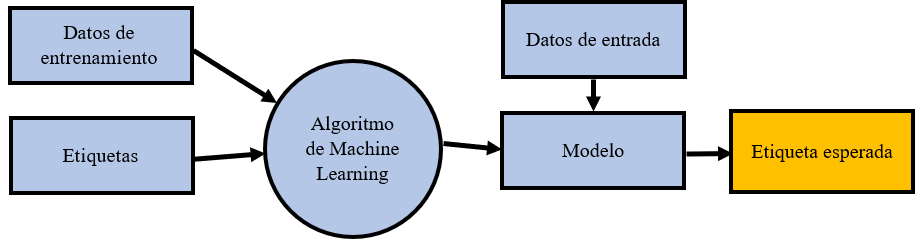
\includegraphics[width=0.80\linewidth]{images/supervisado.PNG}
    \end{center}
    \caption{Modelo de aprendizaje supervisado}
    \label{fig:supervisado}
    \end{figure}
    
    \item \textbf{Aprendizaje no supervisado}: En este tipo de aprendizaje, no se tiene claro cuál será la salida de los modelos \cite{MML2018} y únicamente se conocen los datos de entrada. De esta forma, estos algoritmos intentan encontrar en los datos patrones y clases que puedan ser útiles. Algoritmos comúnmente usados en aprendizaje no supervisado son las redes neuronales o diferentes tipos de agrupamientos (\textit{clustering}) como el algoritmo k-means, normalmente indicado para datos numéricos \cite{Thomas_2020}. En la Figura \ref{fig:nosupervisado} se puede ver un gráfico que muestra el comportamiento descrito.
    
    \begin{figure}[htb]
    \begin{center}
    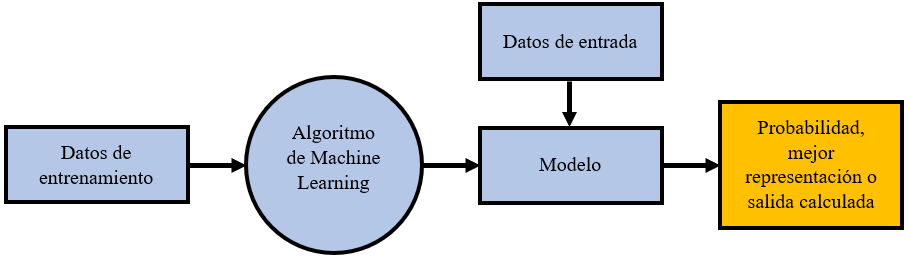
\includegraphics[width=0.80\linewidth]{images/nosupervisado.PNG}
    \end{center}
    \caption{Modelo de aprendizaje no supervisado}
    \label{fig:nosupervisado}
    \end{figure}
    
    \item \textbf{Aprendizaje por refuerzo}: El modelo aprende a base de prueba y error. El modelo (o agente) interactúa con el entorno (contiene las reglas y limitaciones) y va mejorando. El agente, según el estado del entorno, realiza una acción y el entorno responde, entonces, el agente utiliza la información recibida como "recompensa" o "castigo" para orientar su comportamiento de forma que si la respuesta del entorno es positiva (recompensa), el agente reforzará ese comportamiento y si, por el contrario, esta respuesta es negativa (castigo), el agente actuará de forma distinta llegado de nuevo el mismo estado u otro similar \cite{MML2018} \cite{Thomas_2020}. En la Figura \ref{fig:areforzado} se puede ver un gráfico que muestra el comportamiento descrito.
    
    \begin{figure}[htb]
    \begin{center}
    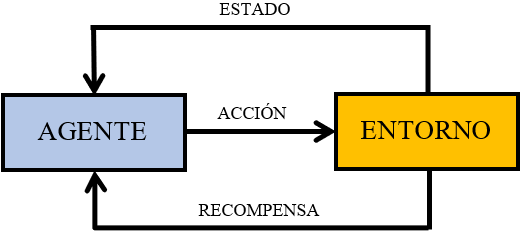
\includegraphics[width=0.45\linewidth]{images/areforzado.PNG}
    \end{center}
    \caption{Modelo de aprendizaje por refuerzo}
    \label{fig:areforzado}
    \end{figure}

     \item \textbf{Aprendizaje semi-supervisado}: El aprendizaje semi-supervisado se aplica cuando una parte de los datos están etiquetados (se conoce la entrada y la salida) y la otra no. Esto puede ocurrir cuando generar datos es un proceso muy costoso \cite{MML2018}. En estos casos, el problema se encuentra entre el aprendizaje supervisado y el no supervisado y se aplican algoritmos como modelos generativos (\textit{generative models}) o métodos basados en gráficos (\textit{graph-based methods}) o máquinas de soporte vectorial semi-supervisadas \cite{Thomas_2020}.
    
\end{itemize}

La utilización de estos tipos depende de las necesidades y del problema que se quiera resolver; en el caso del análisis de malware, el aprendizaje supervisado es el más usado \cite{zero}.

\subsection{Aprendizaje Supervisado}\label{sec:algoritmos}
\noindent La característica que define al aprendizaje supervisado es la disponibilidad de datos de entrenamiento etiquetados. El nombre indica una idea de un ``supervisor'' que instruye al sistema con etiquetas para que pueda asociarlas con los datos de entrada y que posteriormente sea capaz de clasificar otros datos no etiquetados \cite{126}.

El aprendizaje supervisado se puede dividir en dos tipos: clasificación y regresión. Los modelos de regresión se basan en el análisis de relaciones entre tendencias y variables para poder realizar predicciones sobre variables continuas, y los de clasificación asignan etiquetas discretas a observaciones particulares \cite{127}. A continuación, se describirán de forma general los algoritmos de clasificación de aprendizaje supervisado más utilizados en análisis de malware:


\begin{itemize}
\item \textbf{Regresión logística (\gls{LR})}: Es comúnmente empleado para los sistemas de puntuación en aplicaciones y para el modelado de riesgo crediticio \cite{131}. En primer lugar, se realiza una regresión lineal sobre la relación entre variables para obtener el modelo. Después, la función logística se aplicará a la regresión para obtener la probabilidad de que la muestra pertenezca a cada una de las clases y se clasificará en función de la probabilidad más alta. La función logística, también llamada función \textit{sigmoidea}, es una curva en forma de ``S'' que toma cualquier número lo asigna a un valor entre 0 y 1, pero nunca esos valores exactamente \cite{132}. Los trabajos que usan este algoritmo para sus análisis son: \cite{elderan}, \cite{rwguard} y \cite{entropy}.

Para realizar las predicciones, hay que tener en cuenta que la probabilidad debe de transformarse en valores binarios (0 o 1), y para ello se introduce en la ecuación de regresión logística junto con los coeficientes (valores beta) del algoritmo, estimados mediante el método de máxima verosimilitud \cite{133}. Los mejores coeficientes darán como resultado un modelo que prediga un valor muy cercano a 1 para una clase y 0 para la otra.

Para obtener la función de regresión logística se usa la Fórmula \ref{equ:lr} \cite{132}
\begin{equation}\label{equ:lr}
y = \frac{e^{(\beta_0 + \beta_1x)}}{1 + e^{(\beta_0 + \beta_1x)}}
\end{equation}
\noindent donde, $y$ el valor de salida previsto, $\beta_0$ el coeficiente de sesgo o intersección y $\beta_1$ el coeficiente para cada valor de entrada $x$


La Figura \ref{fig:logistic} representa gráficamente todo lo explicado anteriormente. 

\begin{figure}[h!]
\begin{center}
{\scalebox{.7}{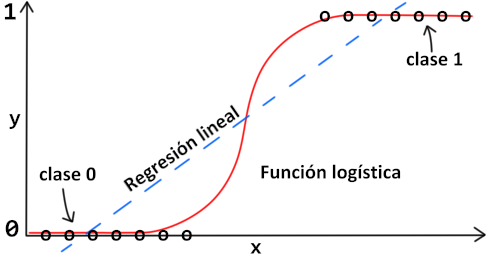
\includegraphics{images/logistic.png}}}
\end{center}
\caption{Gráfico de la regresión logística.}
\label{fig:logistic}
\end{figure}


\item \textbf{Bayesiano ingenuo (\gls{NB})}: Es un clasificador basado en el teorema de Bayes. Almacena la probabilidad previa de cada clase y la probabilidad condicional de cada valor de los atributos. Estima estas cantidades contando la frecuencia de ocurrencia de las clases y de los atributos en los datos de entrenamiento. Después, asumiendo la independencia condicional de los atributos, usa la regla de Bayes para calcular la probabilidad posterior de cada clase dados nuevos datos sin etiquetar \cite{134}. Los trabajos que usan este algoritmo son: \cite{elderan}, \cite{flow}, \cite{shallow}, \cite{rwguard}, \cite{detecting} y \cite{Kok2019}.

Para calcular la probabilidad posterior de la clase se usa la Fórmula \ref{equ:nb} \cite{131}
\begin{equation}\label{equ:nb}
P (clase | datos) = \frac{P (datos | clase)*P (clase)}{P (datos)}
\end{equation}
\noindent donde, $P(clase)$ es la probabilidad previa de una etiqueta, $P(datos | clase)$ es la probabilidad previa de que un conjunto de características dado se clasifique como etiqueta y $P(datos)$ es la probabilidad previa de que apareciera un conjunto de características.


\item \textbf{K-vecinos más cercanos (\gls{KNN})}: Este algoritmo de aprendizaje perezoso clasifica los datos en función de su proximidad con otros mediante funciones de distancia \cite{136}. Ser un algoritmo perezoso significa que no se necesita generalizar los datos de entrenamiento para la generación del modelo \cite{137}. En \gls{KNN}, la ``K'' es el número de vecinos más cercanos y es conveniente que sea impar si hay un número par de clases. Para seleccionar la ``K'' adecuada, se ejecuta el algoritmo \gls{KNN} varias veces con diferentes valores de ``K'' y se elige el valor que reduzca la cantidad de errores y mantenga la capacidad del algoritmo para hacer predicciones con precisión con datos nuevos. La principal desventaja ese algoritmo es que se vuelve más lento a medida que aumenta el número de datos \cite{135}. Los trabajos que usan este algoritmo para construir sus modelos de \gls{ML} son: \cite{shallow} y \cite{detecting}.

La distancia entre los k vecinos se puede calcular con la Fórmula de distancia euclidiana \ref{equ:knn} \cite{143}
\begin{equation}\label{equ:knn}
d(p,q) = \sqrt{\sum_{i=1}^{n} (q_i - p_i)^2}
\end{equation}
\noindent donde, $p$ y $q$ son la posición de dos vecinos cualquiera, $d$ la distancia que queremos calcular y $n$ el número de dimensiones o características.

En la Figura \ref{fig:knn} se puede ver una representación gráfica del algoritmo.

\begin{figure}[h!]
\begin{center}
{\scalebox{.65}{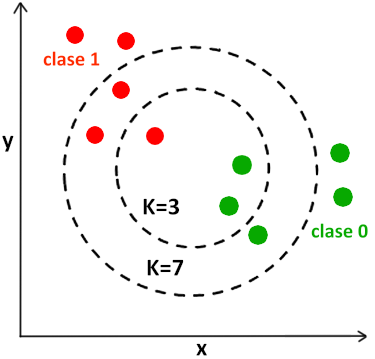
\includegraphics{images/knn.png}}}
\end{center}
\caption{Representación gráfica del algoritmo KNN.}
\label{fig:knn}
\end{figure}

\item \textbf{Árboles de decisión (\gls{DT})}: Proporciona una partición jerárquica de los datos de entrenamiento, donde las 'hojas' o nodos del árbol representan etiquetas y las ramas representan las características o atributos de los datos \cite{141}. El conjunto de datos es dividido en subconjuntos cada vez más pequeños, y esto se repite de manera recursiva hasta que ya no haya más datos por analizar o se cumplan ciertas condiciones, como una profundidad límite. Sigue la estructura del algoritmo \gls{ID3} para determinar la división de los datos \cite{142}. Los trabajos que usan este algoritmo para sus análisis son: \cite{shallow}, \cite{rwguard} y \cite{detecting}.

El algoritmo \gls{ID3} selecciona la mejor característica mientras construye el árbol de decisión. Para esta elección, se usa una métrica llamada mérito o \textit{information gain}, que calcula la reducción de la entropía \cite{144}. La característica con el mayor mérito será la mejor. El mérito de una característica se calcula con la Fórmula \ref{equ:merito}
\begin{equation}\label{equ:merito}
IG(S,a) = E(S) - E(S | a)
\end{equation}
\noindent donde, $IG(S,a)$ es el mérito para el conjunto de datos $S$ para la característica de la columna $a$, $E(S)$ es la entropía del conjunto de datos antes de cualquier cambio y $E(S | a)$ es la entropía condicionada por $a$.


%\st{Para obtener la entrop\'ia se usa la siguiente f\'ormula, donde...} %\textit{E} es la entropía que queremos calcular del es el conjunto de datos o \textit{dataset} \textit{S}, \textit{n} el número total de clases en la columna de destino y \(p_i\) la probabilidad de la clase \textit{i} o la relación entre el número de filas con clase \textit{i} en la columna de destino y el número total de filas en el conjunto de datos \cite{142}:
%\change{modificar el estilo de describir las f\'ormulas por el siguiente. 
%Unificar t\'erminos F\'ormula o Ecuaci\'on utilizas \$ en vez de el comando textit - HECHO}

Para obtener la entropía se usa la Fórmula \ref{equ:entropy} \cite{142}
%\[ E(S) = \sum_{i=1}^{n} - p_i\log_2(p_i) \]
\begin{equation}\label{equ:entropy}
E(S) = \sum_{i=1}^{n} - p_i\log_2(p_i)
\end{equation}
\noindent donde, $E$ es la entropía que queremos calcular del es el conjunto de datos $S$, $n$ el número total de clases en la columna de destino y $p_i$ la probabilidad de la clase $i$ o la relación entre el número de filas con clase $i$ en la columna de destino y el número total de filas del conjunto de datos.

En la Figura \ref{fig:tree} se puede ver un ejemplo de un árbol de decisión sobre préstamos.

\begin{figure}[h!]
\begin{center}
{\scalebox{.34}{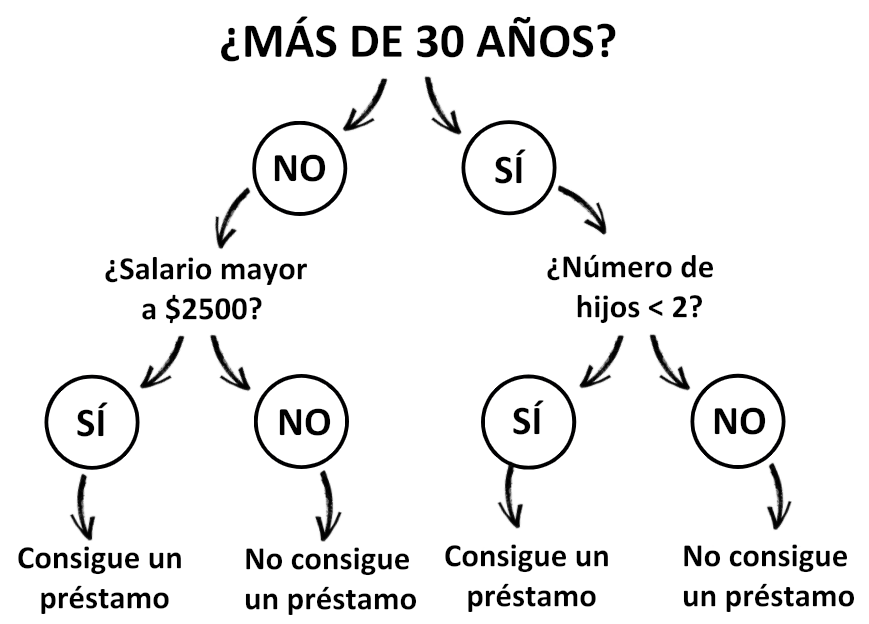
\includegraphics{images/tree.png}}}
\end{center}
\caption{Representación gráfica de un árbol de decisión.}
\label{fig:tree}
\end{figure}

\newpage

\item \textbf{Bosque aleatorio (\gls{RF})}: Como sugiere el nombre, un bosque aleatorio es la fusión de valores aleatorios provenientes de un conjunto de árboles de decisión \cite{138}. Estos árboles de decisión están generalmente entrenados con el método de \textit{``bagging''}, que consiste en la combinación de modelos de aprendizaje para aumentar la precisión del resultado final \cite{140}. Una ventaja de este algoritmo es que se puede utilizar para problemas de clasificación y también para problemas de regresión. Los trabajos que hacen uso de este algoritmo son: \cite{flow}, \cite{traffic}, \cite{sdn}, \cite{rwguard}, \cite{detecting} y \cite{Kok2020}.
%\change{ordenar por fecha las citas ..17, ..18, ..18a, ..19 - HECHO}
Para elegir los valores aleatorios, se buscará la mejor característica en un conjunto aleatorio de características. Se pude incrementar la aleatoriedad aún más mediante el uso de umbrales para cada característica en lugar de buscar las mejores \cite{139}.

La Figura \ref{fig:RF} es una representación gráfica del algoritmo con dos árboles de decisión.

\begin{figure}[h!]
\begin{center}
{\scalebox{.29}{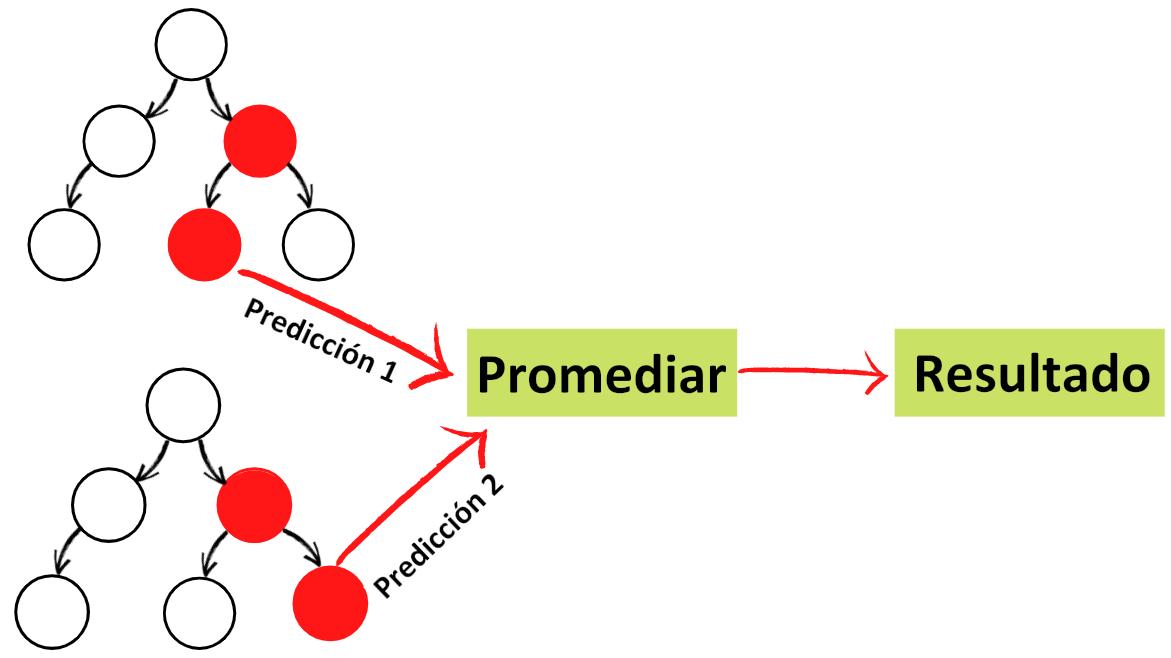
\includegraphics{images/rf.png}}}
\end{center}
\caption{Representación gráfica del algoritmo Bosque Aleatorio.}
\label{fig:RF}
\end{figure}


Para promediar los resultados, se utiliza la Fórmula \ref{equ:rf} \cite{145}
\begin{equation}\label{equ:rf}
RFfi_i = \frac{\sum_{j \in n} normfi_{ij}}{T}
\end{equation}
\noindent donde, $T$ es el número de árboles de decisión, $RFfi_i$ la importancia de la característica $i$ calculada a partir de todos los árboles de decisión $n$ y $normfi_{ij}$ la importancia de la característica $i$ normalizada en el árbol de decisión $j$.


\item \textbf{Máquina de soporte vectorial (\gls{SVM})}:
Una máquina de soporte vectorial clasifica los datos mediante la construcción de un plano de decisión (hiperplano) de N dimensiones que separa los datos en dos categorías, dependiendo de sus características \cite{131}. Los modelos \gls{SVM} están relacionados con las redes neuronales, ya que un modelo que utilice una función sigmoide es equivalente a una red neuronal de perceptrón de dos capas \cite{128}. Un conjunto de características junto con sus etiquetas, que representan las categorías, se llama vector. El objetivo del \gls{SVM} es encontrar el hiperplano óptimo que separe a los vectores según sus categorías. Los trabajos que usan este algoritmo para sus análisis son: \cite{elderan}, \cite{flow}, \cite{shallow}, \cite{detecting} y \cite{entropy}.

Los vectores cercanos al hiperplano se llaman vectores de apoyo, y la distancia entre estos vectores de apoyo se llama margen o \textit{maximal margin} \cite{146}. Es difícil separar datos perfectamente en dos categorías, por lo que se puede permitir cierta flexibilidad en la clasificación con los denominados márgenes blandos o \textit{soft-margins}, introduciendo un nuevo parámetro \textit{c} en la máquina.

\gls{SVM} utiliza un conjunto de funciones matemáticas que se definen como el núcleo o kernel, el cual procesa los datos de entrada y devuelve el producto interno entre dos puntos en un espacio de características de cualquier dimensión \cite{147}. Si los datos se pueden separar con un hiperplano lineal, usamos \gls{SVM} Lineal con kernel lineal. Si ese no es el caso, debemos recurrir a \gls{SVM} No Lineal y usar kernels para transformar espacios no lineales en espacios lineales \cite{148}.

Los diferentes algoritmos de \gls{SVM} utilizan diferentes tipos de kernel. Los más comúnmente usados son los siguientes con sus respectivas ecuaciones: 

\begin{itemize}
    \item \textbf{Lineal}: El más simple de todos, calculado con la Fórmula \ref{equ:l} \cite{150}
    \begin{equation}\label{equ:l}
    k(x_i,x_j) = (x_ix_j+c)
    \end{equation}
    \noindent donde, $(x_i,x_j)$ son los dos puntos en el espacio de características y $c$ es el parámetro de flexibilidad.
    
    \item \textbf{Polinómico}: Usado en el procesamiento de imágenes y calculado con la Fórmula \ref{equ:p} \cite{149}
    \begin{equation}\label{equ:p}
    k(x_i,x_j) = (\alpha x_ix_j+c)^d
    \end{equation}
    \noindent donde, $(x_i,x_j)$ son los dos puntos en el espacio de características, $d$ es el grado del polinomio, $\alpha$ la pendiente y $c$ un parámetro que intercambia la influencia de los términos de orden superior frente a los de orden inferior en el polinomio. Si $c = 0$, el kernel se denomina homogéneo.
    
    \item \textbf{Función de base radial Gaussiana}: Utilizado cuando no hay conocimiento previo sobre los datos y calculado con la Fórmula \ref{equ:rg} \cite{147}
    \begin{equation}\label{equ:rg}
    k(x_i,x_j) = \exp(-\gamma \vert\vert x_i-x_j \vert\vert^2)
    \end{equation}
    \noindent donde, $(x_i,x_j)$ son los dos puntos en el espacio de características y $\gamma$ es la función \gls{RBF}.
    
    \item \textbf{Sigmoide}: Usada para las redes neuronales y calculada con la Fórmula \ref{equ:s} \cite{150}
    \begin{equation}\label{equ:s}
    k(x_i,x_j) = \tanh(\alpha x_ix_j + c)
    \end{equation}
    \noindent donde, $(x_i,x_j)$ son los dos puntos en el espacio de características y $\alpha$ es la pendiente.
\end{itemize}


La  Figura \ref{fig:SVM} muestra una representación gráfica de un ejemplo de \gls{SVM} lineal de dos dimensiones:

\begin{figure}[h!]
\begin{center}
{\scalebox{.3}{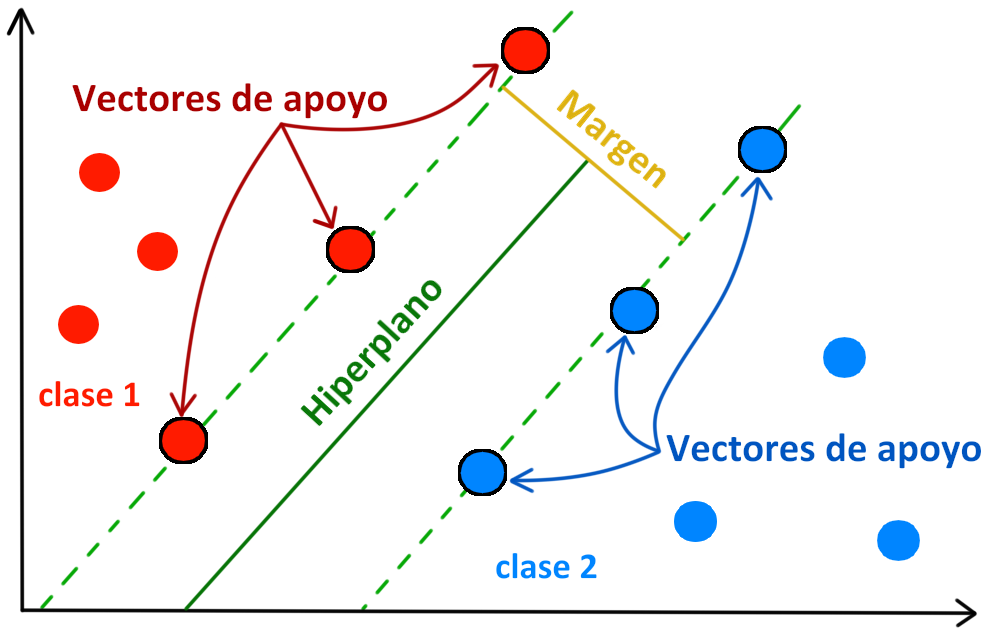
\includegraphics{images/svm.png}}}
\end{center}
\caption{Representación gráfica de SVM lineal de dos dimensiones.}
\label{fig:SVM}
\end{figure}
%\change{unificar el tipo de letra de alas figuras - HECHO}

\end{itemize}

A continuación, se listan las librerías de Python más utilizadas para desarrollar un modelo de \gls{ML}: 

\begin{itemize}
    \item \textbf{Numpy}: Se trata de una de las librerías numéricas más utilizadas para llevar a cabo tanto operaciones matemáticas y lógicas, como ordenado, selección,transformaciones y operaciones estadísticas  sobre \textit{arrays}. Proporciona cantidad de funcionalidades de álgebra lineal, muy útiles en \gls{ML}. Se trata de una librería cuyas operaciones se realizan con gran rapidez, debido a la vectorización: no existe ninguna clase de bucle, indexado, etc. en el código, sino que estas partes más costosas se encuentran por debajo en código C pre-compilado \cite{NMPYDOC}. 
    
    \item \textbf{TensorFlow}: Es una interfaz para expresar algoritmos de \gls{ML}, y una implementación para ejecutarlos. Es un sistema flexible con capacidad para la utilización de una gran cantidad de algoritmos, así como para sistemas heterogéneos y diferentes dispositivos, incluidos móviles, desarrollado por Google \cite{45166}.
    
    \item \textbf{Keras}: Esta librería es muy utilizada para implementar modelos de \textit{deep learning}. Está construida encima de TensorFlow, lo que hace que sea sencilla de utilizar \cite{MML2018}.
     
    \item \textbf{Pandas}: Pandas es un herramienta para explorar, limpiar y procesar datos tabulares, como bases de datos, convirtiéndolos en un tipo de datos concreto, mucho más fácil de manejar, denominado \textit{DataFrame}. Es ampliamente utilizada en modelos de \gls{ML} para obtener una entrada de datos eficiente y eficaz \cite{PNDSDOC}. 
    
    \item \textbf{Matplotlib}: Es una librería utilizada en el campo de la ciencia de datos para visualizar los datos gráficamente. Este aspecto es muy importante para obtener conocimiento de los datos y para razonar los resultados que ofrece el modelo de \gls{ML} \cite{MML2018}.
    
    \item \textbf{Scikit-learn}: Se trata de una librería que proporciona herramientas de \gls{ML} con un entorno para usuarios que no sean expertos. Está enfocada para un uso de propósito general mediante lenguaje de alto nivel. Destaca por su eficiencia, accesibilidad y reusabilidad en varios contextos \cite{sklearn_api}.

\end{itemize}

\subsection{Aplicación del Aprendizaje Automático al Análisis de Malware}

\noindent Cuando se habla del aprendizaje automático en el análisis de malware, es preciso saber que existen diferentes objetivos posibles a conseguir, distintas características a utilizar y cómo extraerlas y el tipo de algoritmo de aprendizaje automático que se utiliza.

Primero, es necesario saber cuál es el objetivo del análisis, que puede ser: la detección de malware (el principal y predominante) para determinar si una muestra es maliciosa; el análisis de similitudes, para estudiar la evolución o variación de las muestras o detectar la pertenencia de una muestra desconocida a una familia; o la detección de categorías de malware, para conocer el objetivo del malware.

Dependiendo del objetivo y del conjunto de datos que se tenga, se hará uso de un tipo concreto de algoritmo de \gls{ML} \cite{Ucci2019}. Esto se puede ver reflejado en el esquema que se muestra en la Figura \ref{fig:esquemaml}.

\begin{figure}[htb!]
\begin{center}
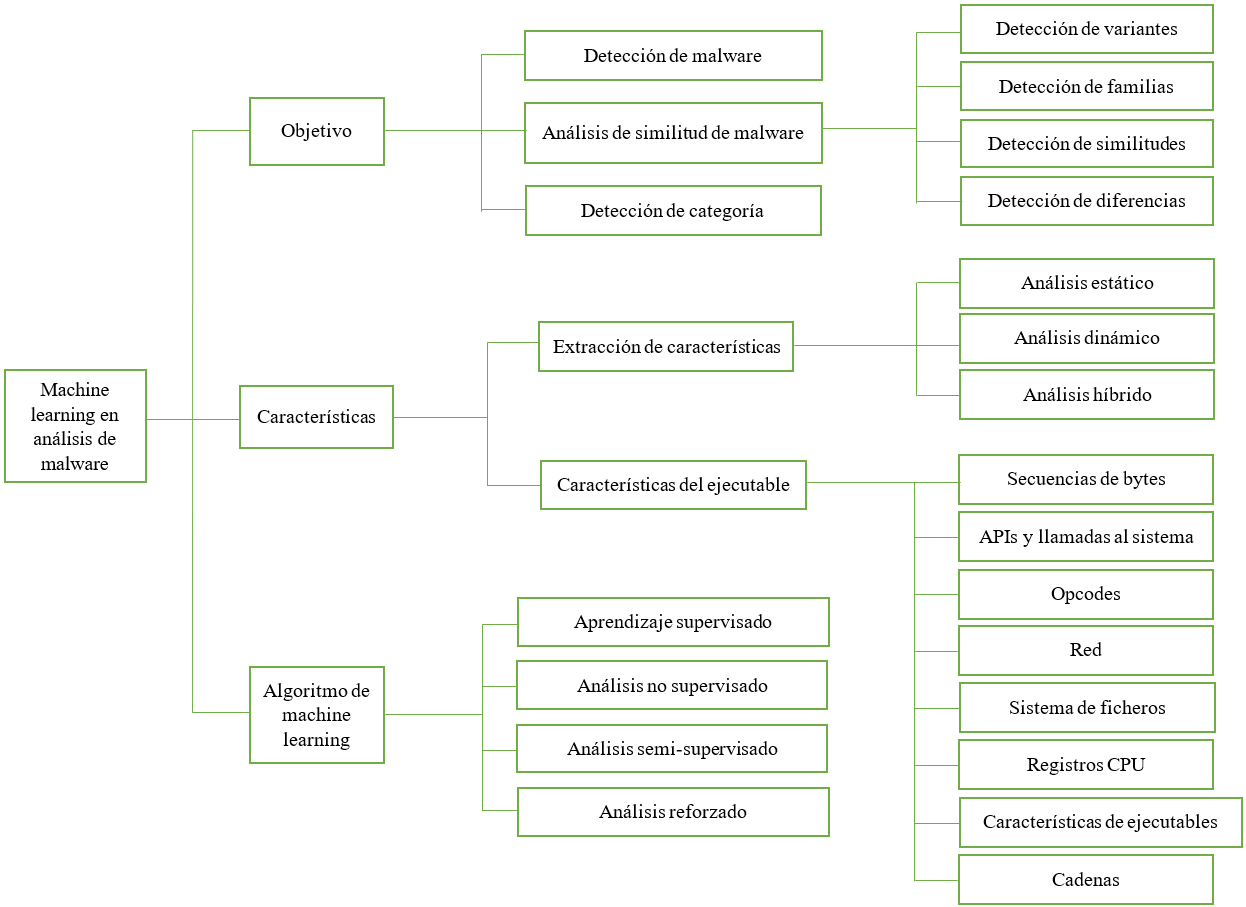
\includegraphics[width=1\linewidth]{images/esquemaml.PNG}
\end{center}
\caption{Taxonomía de las técnicas de ML en el análisis de malware \cite{Ucci2019}}
\label{fig:esquemaml}
\end{figure}

Es importante también conocer las características del ejecutable que se van a utilizar para el análisis, como pueden ser secuencias de bytes, llamadas al sistema y \gls{API}s, actividad de red o cadenas. Todas estas características se extraerán haciendo uso del análisis estático (Sección \ref{sec:aestatico}), del análisis dinámico (Sección \ref{sec:adinamico}) o de la combinación de ambos.

En el caso del análisis de malware y de este trabajo, que está enfocado en detectar programas ransomware, usar un modelo de clasificación es lo más conveniente.
 

%trabajos relaccionados	
\chapter{Estado del Arte}\label{Capitulo4}
\noindent En este capítulo se abordan los trabajos relacionados con el tema de análisis y detección de amenazas de malware y ransomware mediante el uso de algoritmos de aprendizaje automático y otras técnicas mencionadas en el Capítulo \ref{Capitulo3}. Se describirá cómo han creado sus modelos de \gls{ML} y qué resultados han obtenido. Se realiza una distinción entre los estudios cuya finalidad es la detección de malware \ref{sec:trabajosmalware} y aquellos para el análisis de ransomware \ref{sec:trabajosransom}. Al final del capítulo se mostrará una tabla con los trabajos relacionados y los resultados detallados.

\section{Trabajos sobre Análisis de Malware} 
\label{sec:trabajosmalware}

\noindent Konrad Rieck \textit{et al.} (2011) \cite{automatic} proponen un \textit{framework} (entorno o marco de trabajo) para analizar mediante el aprendizaje automático el comportamiento de malware. Este marco permite identificar nuevas clases de malware con un comportamiento parecido (\textit{clustering} o agrupamiento) y asignarlas en una estas clases (clasificación). En la Figura \ref{fig:automatic} se muestra una descripción esquemática de este marco de análisis. Exponen un enfoque para el análisis basado en el comportamiento que puede procesar miles de archivos de malware a diario en un entorno seguro usando CWSandbox. Proponen un mapeo del comportamiento en un espacio vectorial, de modo que los patrones de comportamiento sean accesibles de manera eficiente por las técnicas de aprendizaje automático. El comportamiento que coincide con el de malware conocido se identifica mediante vectores prototipo de clústeres previamente descubiertos, y posteriormente los informes que contienen el comportamiento no identificado se agrupan para descubrir nuevos tipos de malware. Usan dos conjuntos de datos para los experimentos, uno que contiene 3.133 muestras de malware conocido sacado de la página web de CWSandbox, y otro con 33.698 muestras desconocidas obtenidas de Sunbelt Software. Limitan las muestras de cada tipo de malware a 300, las analizan usando CWSandbox, y esto da como resultado 3.133 informes de comportamiento. Su \textit{framework} reduce los requisitos de memoria en un 94\% con un factor de aceleración de 4, lo que permite procesar 33.000 informes de comportamiento de malware en menos de 25 minutos, algo que superaba a los métodos de análisis más avanzados en su día. En los experimentos con uno de los prototipos obtienen una exactitud (\textit{precision}) del 99,6\% y un valor-F (\textit{F-score}) del 95\%.

\begin{figure}[h!]
\begin{center}
{\scalebox{.26}{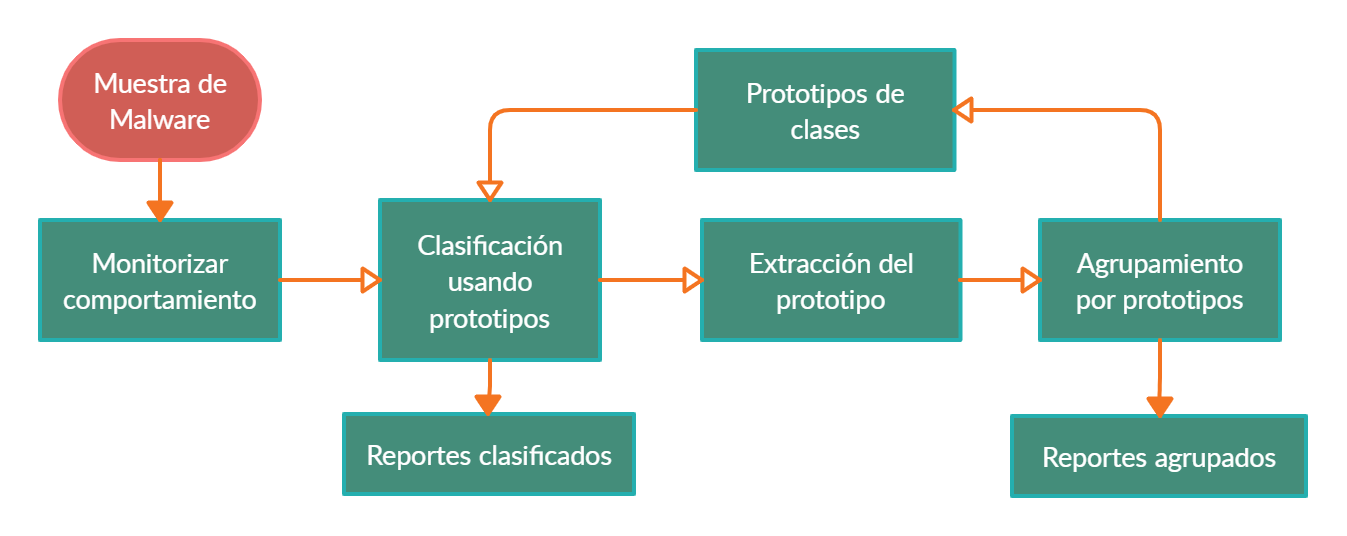
\includegraphics{images/automatic.png}}}
\end{center}
\caption{Descripción esquemática del marco de análisis de Konrad Rieck \textit{et al.}}
\label{fig:automatic}
\end{figure}

\newpage

Mamoun Alazab \textit{et al.} (2011) \cite{zero} proponen un sistema que emplea varias técnicas de minería de datos para detectar y clasificar malware en función de la frecuencia de las llamadas a la \gls{API} de Windows. La metodología general que siguen es la mostrada en la Figura \ref{fig:zero}, donde primero desempaquetan el malware, extraen las \gls{API} y analizan su comportamiento, comparando los resultados con una base de datos de firmas. Después de haber extraído las mejores características, crean el modelo de aprendizaje supervisado para clasificar la muestra (malware o benigno), utilizando algoritmos como \gls{NB}, \gls{KNN}, \gls{DT} y \gls{SVM} con 4 diferentes núcleos. Utilizan la validación cruzada de k iteraciones (\textit{K-fold cross-validation}) para evaluar los resultados del análisis con k = 10. El conjunto de datos consta de 51.223 muestras de malware sacadas de VX Heaven y Honeynet y 15.480 muestras de software benigno. El sistema consigue una tasa de verdaderos positivos (\gls{TPR}) de más del 98,5\% y una tasa de falsos positivos (\gls{FPR}) de menos del 2,5\%, algo que no se había logrado antes.

\begin{figure}[h!]
\begin{center}
{\scalebox{.23}{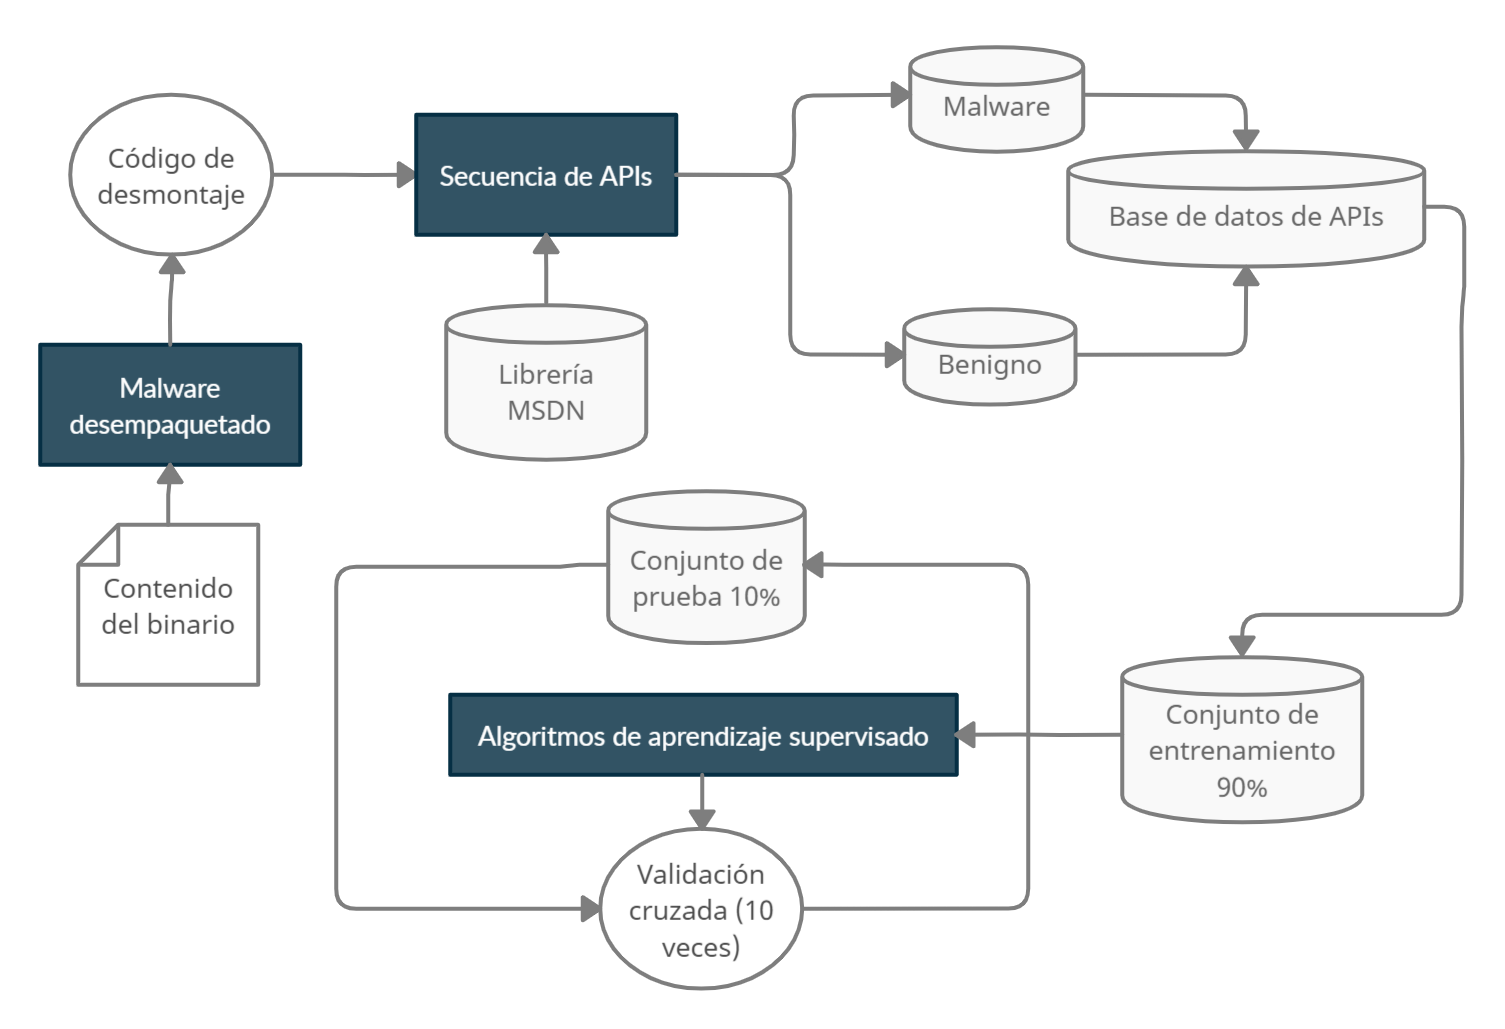
\includegraphics{images/zero.png}}}
\end{center}
\caption{Metodología general del sistema usado en el trabajo de Mamoun Alazab \textit{et al.}}
\label{fig:zero}
\end{figure}


Chandrasekar Ravi \textit{et al.} (2012) \cite{ravimalware} proponen un sistema de detección de malware que modela la secuencia de llamadas de la \gls{API} de Windows con una cadena de Markov de tercer orden. La Figura \ref{fig:ravi} es una representación de la arquitectura de este sistema. Usan algoritmos de clasificación basados en asociación y monitorizan un subconjunto mínimo de categorías de \gls{API} para asegurar la eficiencia del sistema. La novedad que introducen es el proceso de aprendizaje iterativo combinado con la monitorización del comportamiento del programa sospechoso en tiempo de ejecución, creando un sistema dinámico de detección de malware que consta de 3 fases de aprendizaje: offline, online e iterativo. La fase offline están constituida por los siguientes componentes: un conjunto de datos (\textit{dataset}), un rastreador de llamadas de las \gls{API}, una base de datos con los índices de las \gls{API}, una base de datos de firmas, un generador de reglas y una base de datos de reglas. El conjunto de datos contiene 179 muestras de varios tipos de malware y 94 programas benignos. La fase online consta de: el proceso sospechoso que se va a analizar, un rastreador de llamadas de las \gls{API} para ese proceso en específico, una base de datos con los índices de las \gls{API} y el clasificador. El clasificador asigna una etiqueta (benigno o malware) al proceso, utilizando la secuencia rastreada de llamadas a las \gls{API} y las reglas generadas en la fase offline. En la fase iterativa, después de cada clasificación, la etiqueta asignada y la secuencia de las \gls{API} del proceso analizado se agregan iterativamente a la base de datos de firmas. Esto mejorará el modelo de entrenamiento al tener más información para comparar con otros procesos en el futuro. El rendimiento de este sistema supera a los sistemas de detección de malware existentes de la época, con una precisión (\textit{accuracy}) del 90\%.

\begin{figure}[h!]
\begin{center}
{\scalebox{.33}{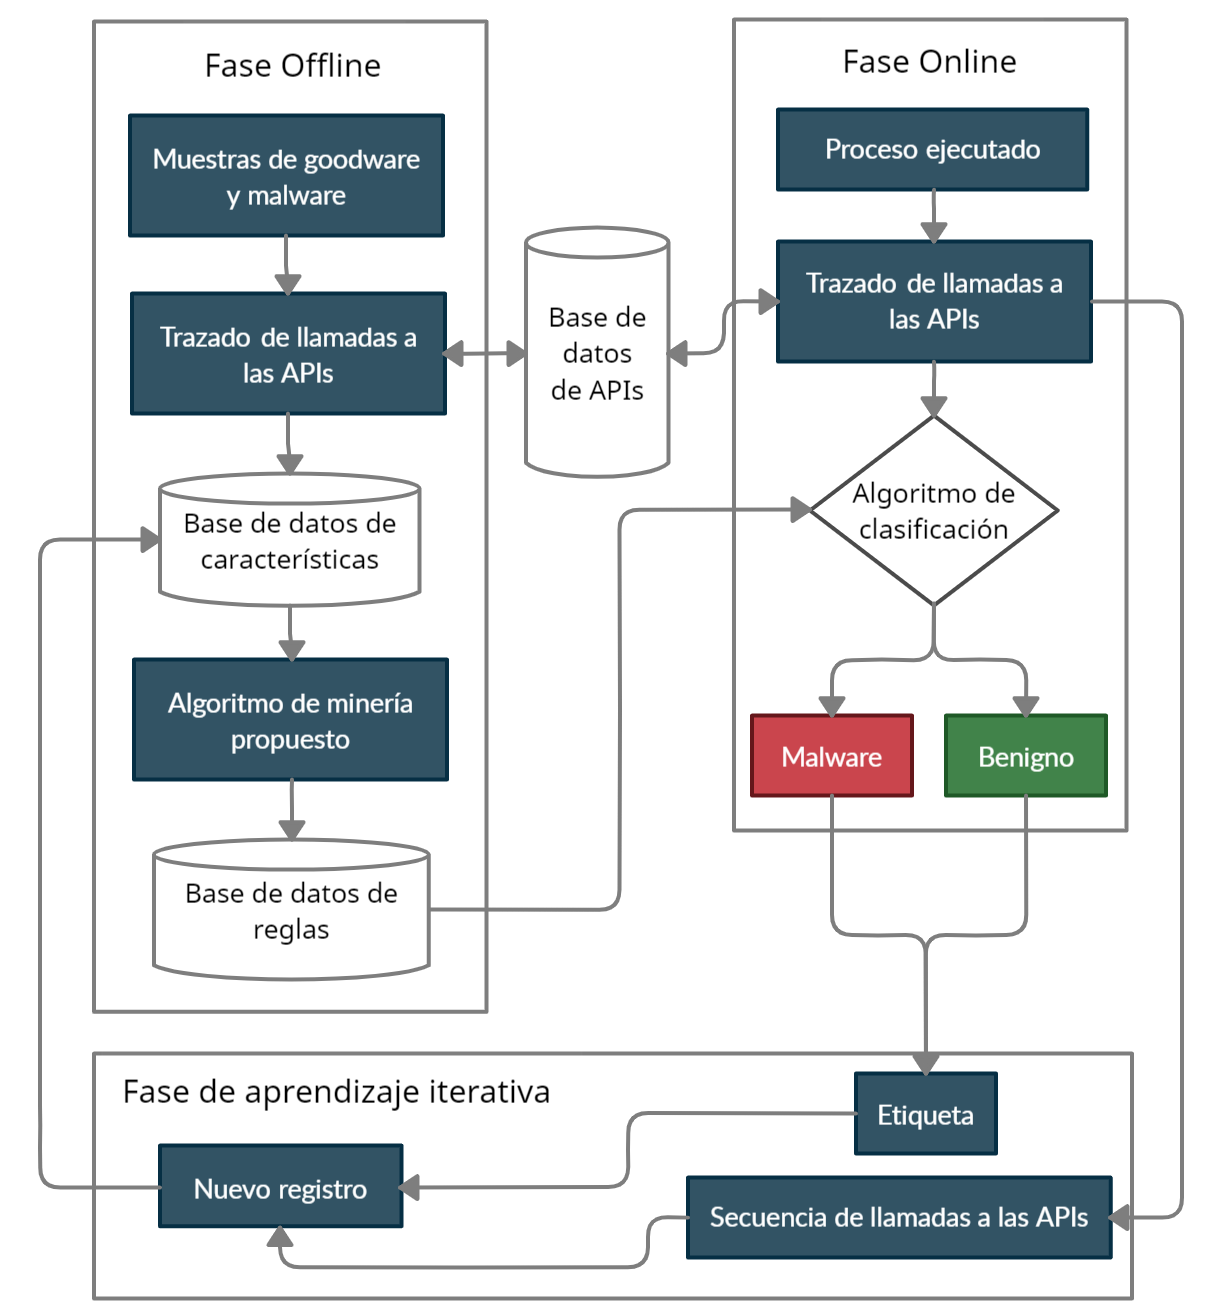
\includegraphics{images/ravimalware.png}}}
\end{center}
\caption{Arquitectura del sistema de detección de malware propuesto por Chandrasekar Ravi \textit{et al.}}
\label{fig:ravi}
\end{figure}


\section{Trabajos sobre Análisis de Ransomware}
\label{sec:trabajosransom}
\subsection{Trabajos que Utilizan Características Heterogéneas}
\noindent En esta sección se agrupan diversos trabajos con métodos heterogéneos para la detección de ransomware distintos a los que se van a utilizar en este estudio, pero de los cuales se puede obtener información relevante.

Amin Kharaz \textit{et al.} en \cite{197235} (2016) realizan un estudio analizando 148.223 muestras de malware reciente, mostrando que el sistema es capaz de detectar correctamente 13.367 muestras de ransomware de diferentes familias, 7.572 de ellas eran desconocidas previamente y no habían sido detectadas por ningún antivirus. 

Se trata de una aplicación que se acopla al sistema al driver del sistema de ficheros, permitiendo su monitorización. 
Además, se combina con la creación de un entorno artificial, que detecta cambios en el escritorio para la detección de ransomware Lockscreen. Este ha de ser lo más realista posible: los datos tienen que ser reales, válidos y no deterministas para no ser reconocidos por los atacantes. Para cada extensión de archivos presente en el sistema de usuario, se crean un número aleatorio de archivos con cabeceras válidas y contenido usando bibliotecas estándar y \textit{queries} de palabras en inglés obteniendo 100.000 frases distintas. Al igual se tiene precaución a la hora de crear los directorios y su estructura de forma realista y no determinista. Se lleva a cabo un algoritmo estadístico para establecer las fechas de creación, modificación y acceso.
En cuanto a la monitorización de sistema de archivos se observa que existen patrones repetidos, usan diferentes estrategias para evitar el acceso a los archivos, hay tres patrones diferenciados que aparecen en la Figura \ref{fig:im12}. Se comprueba la entropía de los archivos en las operaciones de entrada y salida, en lugar de las llamadas a la \gls{API} de Windows, para saber si están siendo cifrados. Se realiza mediante el \textit{framework} Windows Filesystem Minifilter Driver, del kernel de Windows. Esto permite que Unveil este localizado en la capa más cercana posible al \textit{Filesystem}.

\begin{figure}[h!]
\begin{center}
{\scalebox{.825}{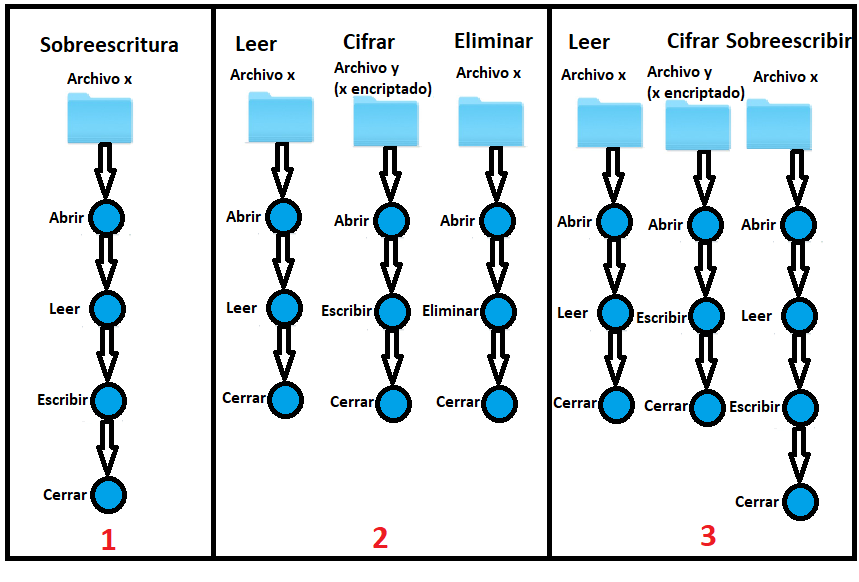
\includegraphics{images/unveil2.png}}}
\end{center}
\caption{Patrones del ransomware para cifrar archivos: 1- El atacante sobrescribe el fichero del usuario con la versión cifrada. 2- El atacante lee un fichero, lo cifra en otro distinto y elimina el original. 3- El atacante lee un fichero, crea una nueva versión cifrada, sobrescribiendo el fichero original }
\label{fig:im12}
\end{figure}

Por otro lado, la detección de Lockscreens se realiza mediante capturas de pantalla de antes y después de ejecutar la muestra y se realizan métodos de análisis de imágenes para comprobar si una gran parte de la pantalla ha cambiado repentinamente, como intensidad de los \textit{pixels}, contraste, dependencias de los píxeles cercanos,etc. También se realiza el análisis del texto de la pantalla en búsqueda de palabras claves de un mensaje de extorsión.

Amin Kharraz \textit{et al.} (2017) en \cite{AminK2017} proporcionan una defensa ante ataques ransomware, garantizando cero pérdidas de datos. Es una solución \textit{end-point} sin limitación ya que está diseñado para proteger los archivos originales intactos ofreciendo recuperación total de datos si ocurre un ataque. Además, no depende de ninguna técnica para identificar funciones de cifrado.
En la investigación de este proyecto se asume que el ransomware puede emplear cualquier técnica para atacar máquinas, es decir, puede emplear estrategias para evadir la detección, comprometer máquinas vulnerables y atacar ficheros. También se asume que el proceso puede emplear cualquier sistema de cifrado personalizado o estándar, así como longitudes de clave arbitrarias. Sumado a esto, se plantea que el usuario puede instalar programas de fuentes no fiables y así el código malicioso puede ejecutarse con privilegios del usuario.

Redemption media el acceso al sistema de ficheros y redirige cada petición de escritura a un área protegida para ejecutar la acción en un archivo reflejado sin cambiar el estado del archivo original. De esta forma, cuando se sabe que no supone un riesgo de ransomware, se aplican los cambios al archivo original. Redemption sabe que la acción no es maliciosa basándose en una puntuación que establece al proceso (usando como métricas la entropía, la operación de borrado y la reescritura de contenido) y que compara con un umbral establecido.

Este sistema hace mucho énfasis en garantizar la consistencia de los datos, por ejemplo cuando el sistema se cuelga, si los metadatos no están actualizados, el sistema trata los cambios como incompletos y descarta los cambios realizados retrocediendo y vuelve a repetir la acción.

En cuanto a los resultados, Redemption detecta ransomware en todas las familias de ransomware utilizadas para las pruebas, con una media de observación de 5 ficheros, no encontrando problemas si el sistema no ha sido entrenado con ciertas familias desconocidas. Además, se obtiene que las aplicaciones tan solo tardan un 2,6\% más en completar sus tareas por utilizar Redemption, demostrando su eficiencia y el ligero impacto al rendimiento.

Shagufta Mehnaz \textit{et al.} (2018) en \cite{Mehnaz2018} exponen que la mayoría de herramientas de detección de ransomware no son capaces de reconocer el agente maligno en tiempo real, lo que conlleva el cifrado de los archivos que luego y las técnicas de descifrado actuales están limitadas, y tienen una tasa de falsos negativos elevada: no son capaces de distinguir el malware de grandes operaciones con archivos como el cifrado benigno o la compresión. RWGuard es una herramienta que cumple los siguientes puntos:
\begin{enumerate}
\item Emplea técnicas de señuelo. Se colocan archivos falsos en nuestro sistema, que el usuario nunca va a escribir. Por lo tanto, si se detecta alguna operación con ellos se deduce al instante que estamos siendo atacados.
\item Monitoriza los procesos en ejecución, así como el sistema de ficheros.
\item Omite los cambios benignos del usuario en los archivos (\textit{file change monitoring}): mediante un mecanismo que monitoriza las propiedades del archivo modificado. Además se utiliza CryptoAPI para que los usuarios y las aplicaciones modifiquen los archivos, así si se producen llamadas a ésta, sabremos que es un cifrado benigno.
\end{enumerate}
El tiempo medio del sistema para la detección de todos los procesos malignos del ransomware es de 8.87 segundos. Se puede descifrar los datos de ataques realizados por las familias Locky, CryptoWall, y CryptoLocker, ya que se pueden recuperar los parámetros del cifrado (como la clave de descifrado) de las llamadas a las funciones criptográficas debido a la monitorización que se realiza. 

Las limitaciones del sistema residen en que está basado en el registro de llamadas \gls{IRP} y actividad de archivos. El lapso de tiempo entre el registro de estas actividades y su análisis en busca de anomalías proporciona una pequeña ventana para que el ransomware pueda realizar sus actividades malignas.

Fei Tang \textit{et al.} (2020) en \cite{TANG2020101997} proponen un sistema cuya finalidad es detectar ransomware de cifrado, basándose en la técnica de introspección de máquina virtual \gls{VMI}. Esta técnica permite, monitorizar cualquier operación que se realiza tanto en el sistema de ficheros como en la comunicación de red, mediante la utilización de máquinas virtuales, en este caso con una Windows 7, de forma que el sistema que queremos defender no se infecta por el malware. El sistema se ha de establecer fuera del sistema operativo. En otro caso, el programa malicioso podría escalar privilegios en el sistema y podría ejecutar órdenes o eliminar/modificar archivos. En este trabajo se explica cómo se realiza el escalado de privilegios y cómo poder detectarlo.

La técnica que emplean para la detección del ransomware se basa en calcular la entropía de los datos escritos en los ficheros, puesto que los datos cifrados tienen un alto valor, y se comparan con un umbral definido para conocer si el sistema de ficheros está siendo atacado por ransomware de cifrado.

También cabe destacar la monitorización de las redes, a través de la cual se puede rastrear la forma en que los atacantes obtienen de servidores remotos las claves de cifrado y posteriormente pueden enviarlas. 

El sistema predice el 100\% de los patrones de entrada/salida provocados en el sistema de ficheros por el ransomware, y tan solo en un 6,23\% de los ejemplos no se apreció ninguna comunicación por red producida por el ransomware. Sumando la capacidad de detección de estas técnicas, teniendo en cuenta falsos negativos y positivos, se calcula una precisión del 100\% en las muestras utilizadas.

En cuanto a las limitaciones, este estudio solo se centra en una serie de patrones tanto del sistema de ficheros como de la red, por lo tanto, pueden existir ejemplos de ransomware que utilicen diferentes patrones o modos de operación. Por otro lado, tampoco es posible recuperar los datos cifrados porque no se realiza la detección en tiempo real.

Amos Ren \textit{et al.} (2020) en \cite{Ren2020} proponen como objetivo aislar los archivos potencialmente maliciosos (fundamentalmente el ransomware de la familia Petya) en máquinas virtuales antes de que dañen el equipo mediante un sistema de seguridad en tres niveles. 

El primer nivel se trata de una extensión para navegador web que detecta las páginas que intenta descargar cualquier contenido sin autorización, bloqueando el sitio. Está construido mediante dos capas:
\begin{enumerate}
    \item La primera capa usa un método híbrido de detección basado en firmas, que permite analizar las propiedades sintácticas y estructurales del programa.
    \item La segunda capa utiliza una detección basada en anomalías, que es capaz de detectar nuevos tipos de malware.
\end{enumerate}

El segundo nivel hace uso de las máquinas virtuales para crear un entorno seguro, dentro del que actúa el tercer nivel, que usa soluciones anti-ransomware para escanear los archivos y eliminar las amenazas que hayan pasado los niveles anteriores.

La creación del entorno seguro además provoca que el atacante piense que el ataque ha sido exitoso, evitando así un segundo ataque. La solución se basa en la creación de un entorno virtual individual para cada descarga, para evitar infecciones de entornos seguros por parte de entornos infectados. 

La limitación fundamental de este sistema reside en la dificultad de los ordenadores actuales en ejecutar varias máquinas virtuales al mismo tiempo, por lo que solo se permiten 4 descargas simultaneas.


Firoz Khan \textit{et al.} (2020) exponen en \cite{9121260} una nueva técnica para la detección de ransomware basadas en secuencias de \gls{DNA} digital, rechazando aquellas basadas en firmas.

Este mecanismo primero selecciona las características para generear la secuencia de \gls{DNA} digital y posteriormente clasificarlas mediante un algoritmo de \gls{ML}, como se aprecia en la Figura \ref{fig:adn}. 
\begin{figure}[h!]
\begin{center}
{\scalebox{.76}{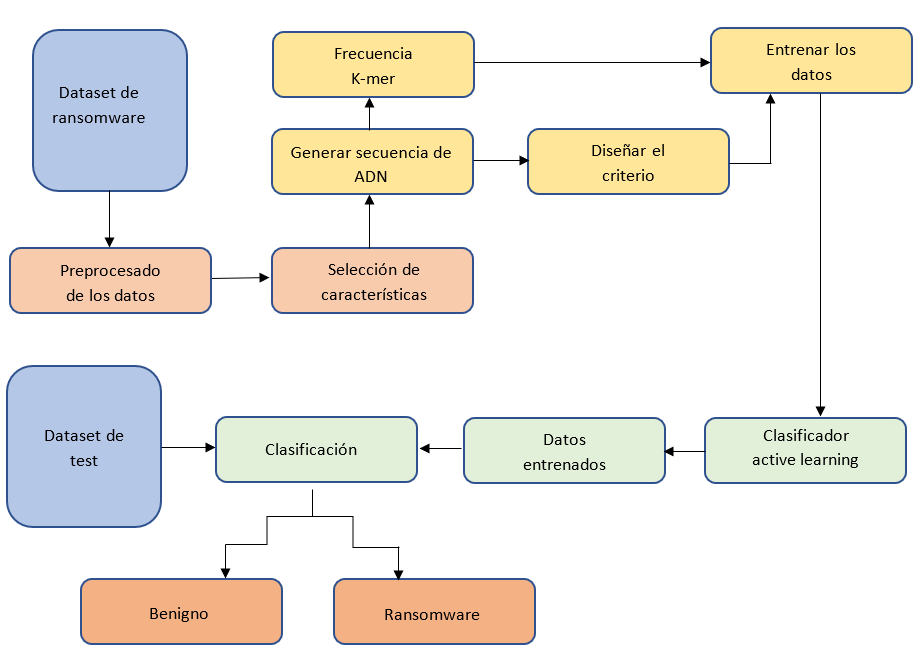
\includegraphics{images/adn.png}}}
\end{center}
\caption{Diagrama de secuencia del proyecto}
\label{fig:adn}
\end{figure}
El \gls{DNA} se usa para construir proteínas y otros componentes celulares de los seres vivos. Está compuesta por largas cadenas conformadas por las bases nitrogenadas: Adenina (A), Guanina (G), Citosina (C) y Timina (T).  Para la creación de la secuencia de \gls{DNA} digital, se realiza una correspondencia binaria para mapear estas moléculas como se observa en la Tabla \ref{tab:moleculas}.


\begin{table}[htb!]
    \centering
    \scriptsize %para hacer la tabla mas pequeña
    \caption{Mapeo de las bases nitrogenadas en código binario}
    \begin{tabular}{|m{3cm} | m{3cm}|}
        \hline
        \rowcolor[HTML]{C0C0C0} 
        \textbf{Codificación} & \textbf{Moléculas}\\ \hline
        00 & A\\ \hline
        01 & C \\ \hline
        10 & G\\ \hline
        11 & T\\ \hline
    \end{tabular}
    \label{tab:moleculas}
\end{table}

Posteriormente, se generan secuencias de \gls{DNA} digital de manera aleatoria para entrenar un modelo de \gls{ML}. Se utiliza \textit{active learning}, un método por el que se pueden realizar consultas de manera interactiva para etiquetar nuevos datos con su salida deseada. Finalmente, se usan algoritmos de clasificación (\gls{NB}, \gls{RF} y Optimización Mínima Secuencial) para detectar las familias de ransomware. 

El \textit{dataset} utilizado se compone de 1524 muestras, de las cuales 582 pertenecen a ransomware y 942 a goodware, con un total de 30970 características.

\subsection{Trabajos que Utilizan Llamadas a la API de Windows}

\noindent En esta sección se agrupan los trabajos que usan las llamadas a la \gls{API} de Windows como característica para desarrollar sus modelos, al igual que este trabajo.

Daniele Sgandurra \textit{et al.} (2016) \cite{elderan} presentan EldeRan, un sistema que usa un algoritmo de aprendizaje automático para clasificar y analizar ransomware dinámicamente. EldeRan se basa en la observación de que las muestras de ransomware suelen realizar acciones que son únicas o significativas con respecto a las realizadas por un programa benigno. Por lo tanto, EldeRan monitoriza los programas sospechosos en sus primeras fases de instalación en un entorno controlado con Cuckoo Sandbox, comprobando si sus acciones coinciden con las que haría un ransomware. La Figura \ref{fig:elderan} representa este sistema. Analizan un conjunto de datos descargados de VirusShare que contiene 582 muestras de ransomware pertenecientes a 11 familias y 942 aplicaciones benignas. A partir de estos datos, se analizan las siguientes características: llamadas a la \gls{API} de Windows, operaciones de clave de registro y del sistema de archivos (lectura, apertura, escritura y eliminación), el conjunto de operaciones realizadas con cierta extensión, operaciones de directorio, archivos eliminados (es decir, el conjunto de archivos que se eliminan por una aplicación durante su instalación) y las cadenas de caracteres incrustadas en el archivo. Todas las funciones, excepto las cadenas, se recopilan mientras se analiza dinámicamente el ransomware. Después de esta fase de análisis, se aplica un algoritmo de selección de características para seleccionar las más relevantes. Por último, las matrices que contienen estas características se utilizan en un clasificador \gls{LR} regularizado que devuelve si es ransomware o un archivo benigno. EldeRan no se basa en firmas, por lo que no necesita tener conocimientos previos de ransomware y puede detectar nuevas familias. Comparan EldeRan con los algoritmos \gls{SVM} y \gls{NB} y demuestran que el rendimiento máximo de estos algoritmos se alcanza con 400 características. Por lo tanto, agregar más características no mejora la precisión, por lo que la selección de características es importante para reducir la complejidad de los algoritmos de aprendizaje automático sin afectar el rendimiento. EldeRan alcanza un área bajo la curva \gls{ROC} del 99,5\% y tiene una tasa de fallos de 2,4\%, inferior a la de \gls{SVM} (4,2\%) y \gls{NB} (8,0\%).

\begin{figure}[h!]
\begin{center}
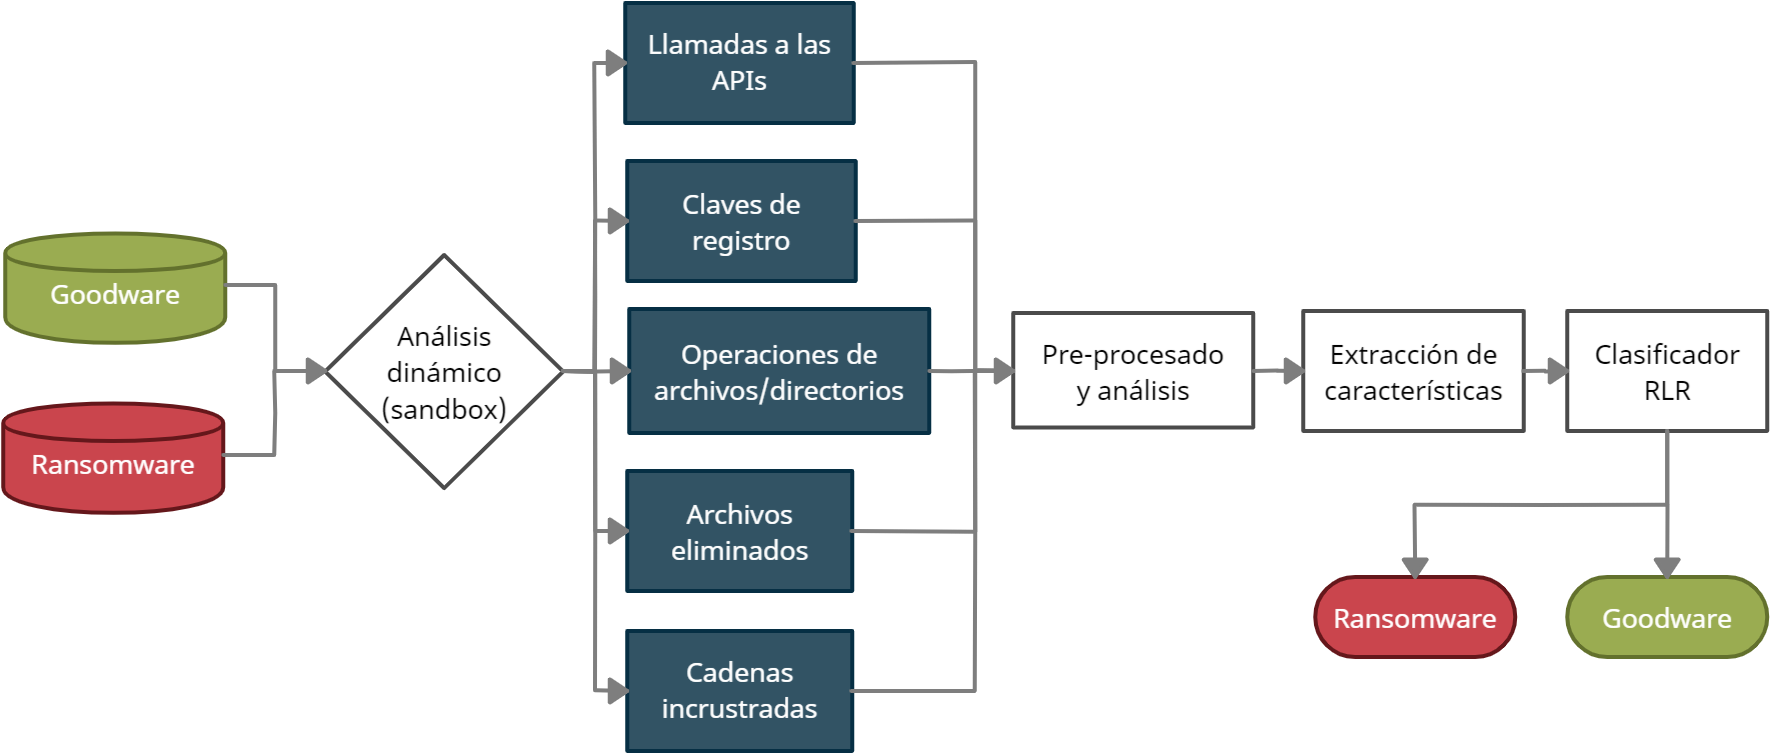
\includegraphics[width=1\linewidth]{images/elderan.png}
\end{center}
\caption{Representación del sistema EldeRan \cite{elderan}}
\label{fig:elderan}
\end{figure}

\newpage

Zhi-Guo Chen \textit{et al.} (2017) \cite{flow} proponen un sistema dinámico representado en la Figura \ref{fig:flow} que utiliza gráficos de flujo de llamadas \gls{API} (\gls{CFG}) y algoritmos como \gls{RF}, \gls{SVM}, \gls{NB} y \gls{LR} para detectar programas ransomware conocidos y desconocidos. Este sistema utiliza la herramienta \textit{API Monitor} para recopilar los datos de las llamadas a las \gls{API} que realiza el programa sospechoso cuando se ejecuta en una máquina virtual. Después, el sistema genera los \gls{CFG} para representar el comportamiento del programa y convierte estos gráficos en vectores de características etiquetados. Posteriormente selecciona el mínimo número de características para reducir el tiempo de la fase de aprendizaje y mejorar el rendimiento. Por último, se usan los algoritmos anteriormente mencionados para construir el modelo de detección que prediga si un programa es ransomware o no, entrenándolo con los vectores de características generados. 

\begin{figure}[h!]
\begin{center}
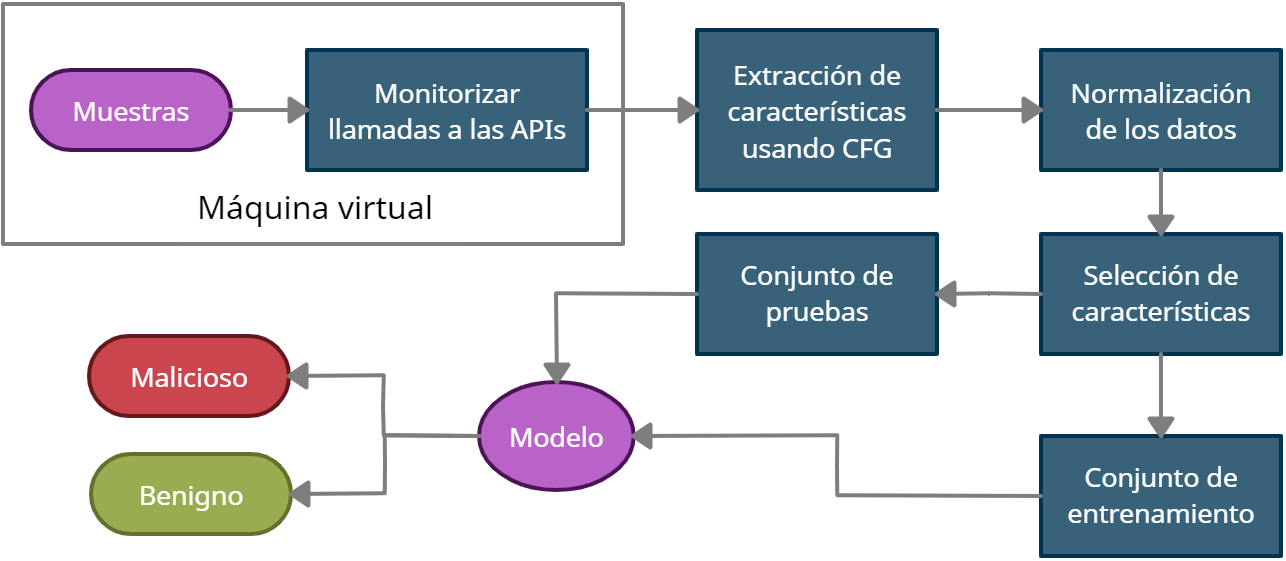
\includegraphics[width=0.9\linewidth]{images/flow.png}
\end{center}
\caption{Representación del sistema dinámico de detección de ransomware \cite{flow}}
\label{fig:flow}
\end{figure}

Hacen uso de la validación cruzada de k iteraciones (\textit{K-fold cross-validation}) para entrenar y probar el modelo. Esta validación consiste en dividir aleatoriamente el conjunto de datos original en k subconjuntos de igual tamaño, usando los k-1 conjuntos para el entrenamiento y el conjunto restante para las pruebas. Este proceso se repite k veces para que todos los subconjuntos se usen para las pruebas una vez. En este trabajo, se realiza la validación con k = 10. Tras varios experimentos, los mejores resultados se obtienen cuando se normalizan los datos y se aplican criterios de correlación y ganancia, obteniendo un 98,2\% en precisión (\textit{accuracy}) y un 97,6\% en \gls{TPR} con el algoritmo \gls{LR}. En cuanto al conjunto de datos usado, recopilan 83 muestras de ransomware diferentes y 85 muestras de software benigno.


Vinayakumar R \textit{et al.} (2017) \cite{shallow} proponen un sistema con una red neuronal profunda, en específico un perceptrón multicapa (\gls{MLP}), para la detección y clasificación de ransomware, usando las llamadas a las \gls{API}, algo que usan todos los trabajos. Analizan 7 familias de ransomware diferentes que han sacado de diversas fuentes, como Open Malware, Contagio Malware Dump, Malwr, theZoo, VirusTotal y VirusShare, recopilando un total de 755 muestras de ransomware y 219 de software benigno. Consideran alrededor de 131 llamadas \gls{API} sacadas de los registros de Cuckoo Sandbox tras analizar las muestras con dicha herramienta. La red \gls{MLP} es una función parametrizada, lo que significa que la \gls{TPR} de ransomware depende de los parámetros óptimos, la cantidad de capas ocultas, número de unidades, la tasa de aprendizaje, etc. Todos los experimentos con \gls{MLP} se realizan en tres capas con 1000, 500 y 250 unidades y se ejecutan con 500 ciclos de aprendizaje (llamados \textit{epochs}), con una tasa de aprendizaje entre 0,01 y 0,5. Este sistema alcanza una precisión (\textit{accuracy}) de 1,0 para detectar si un programa es ransomware o no.

Yuki Takeuchi \textit{et al.} (2018) \cite{detectingSVM} proponen un sistema de detección de ransomware utilizando máquinas de soporte vectorial (\gls{SVM}) y transformando las llamadas \gls{API} que realiza en ransomware en un conjunto de datos vectoriales. A diferencia de las soluciones existentes, este sistema propuesto analiza en profundidad el historial de llamadas a las \gls{API} con más detalle, demostrando una mejora en la \gls{TPR} correcta de ransomware. Usan \gls{SVM} porque generalmente tiene una generalización más alta que los otros algoritmos. La generalización es la capacidad de predecir datos desconocidos, y en este caso es muy útil para detectar ransomware desconocido, ya que no siempre se tienen muestras de todos los tipos posibles de ransomware. Ejecutan 276 muestras de ransomware y 312 muestras de programas benignos o \textit{goodware} en un entorno controlado y seguro con Cuckoo Sandbox, como se ha visto en anteriores trabajos. Después de la ejecución, Cuckoo Sandbox genera reportes que no solo contienen las llamadas a la \gls{API} de Windows, sino también los accesos a los archivos, los árboles de procesos, etc. A partir de estos reportes, solo se extraen las llamadas a la \gls{API} y se guardan como vectores que serán usados en \gls{SVM}. Para evaluar el sistema, usan la métrica de precisión (\textit{accuracy}) y obtienen un 97,48\%. También calculan la tasa de fallos, que es el número de falsos negativos (\gls{FN}) entre el número total de muestras, obteniendo un 1,64\%.

Seong Il Bae \textit{et al.} (2019) \cite{detecting} proponen un sistema de detección de ransomware en un entorno virtual en Windows 7 utilizando VMware que pueda distinguir entre ransomware y archivos benignos, así como entre ransomware y malware. Afirman que los métodos de detección de malware basados en firmas tienen dificultades para detectar ataques de día cero, por lo que no son adecuados para proteger los archivos de los usuarios. Por lo tanto, plantean un nuevo mecanismo de protección especializado que se centra en operaciones específicas de ransomware para poder diferenciarlos de otros malware y archivos benignos. La Figura \ref{fig:detecting} muestra el diagrama de flujo del sistema propuesto. En este trabajo extraen las secuencias de invocación de la \gls{API} de Windows mediante la herramienta intel PIN tool que realizan 1000 archivos de ransomware, 900 archivos de malware y 300 archivos ejecutables benignos. Si el tamaño del reporte de las llamadas es inferior a 10 KB, el reporte se descarta, ya que consideran que el archivo no se ejecutó correctamente. Con esa información generan los vectores de características utilizando un conjunto de n-grama, una subsecuencia de n elementos, y valores de \gls{CF-NCF}, un indicador para modelos de clasificación basado en \gls{TF-IDF}, que es un algoritmo que permite medir la importancia de una palabra en un conjunto de documentos. El rango del valor n de n-grama es entre 1 y 4, ya que comentan que las matrices se vuelven demasiado grandes para ser calculadas cuando n es mayor a cuatro. Posteriormente usan seis algoritmos de aprendizaje automático para crear su modelo de \gls{ML} con los vectores de características generados. Los seis algoritmos que utilizan son: \gls{RF}, \gls{LR}, \gls{NB}, descenso de gradiente o \gls{SGD}, \gls{KNN} y \gls{SVM}. Se realiza una validación cruzada a los datos de entrenamiento, que constituyen el 80\% del \textit{dataset}, y a los de test, el 20\% restante. Dichos procesos de entrenamiento y test fueron repetidos 5 veces. Al realizar sus experimentos con todos los algoritmos, consiguen una precisión (\textit{accuracy}) de entre 97\% y 98,65\%.

\begin{figure}[h!]
\begin{center}
{\scalebox{.3}{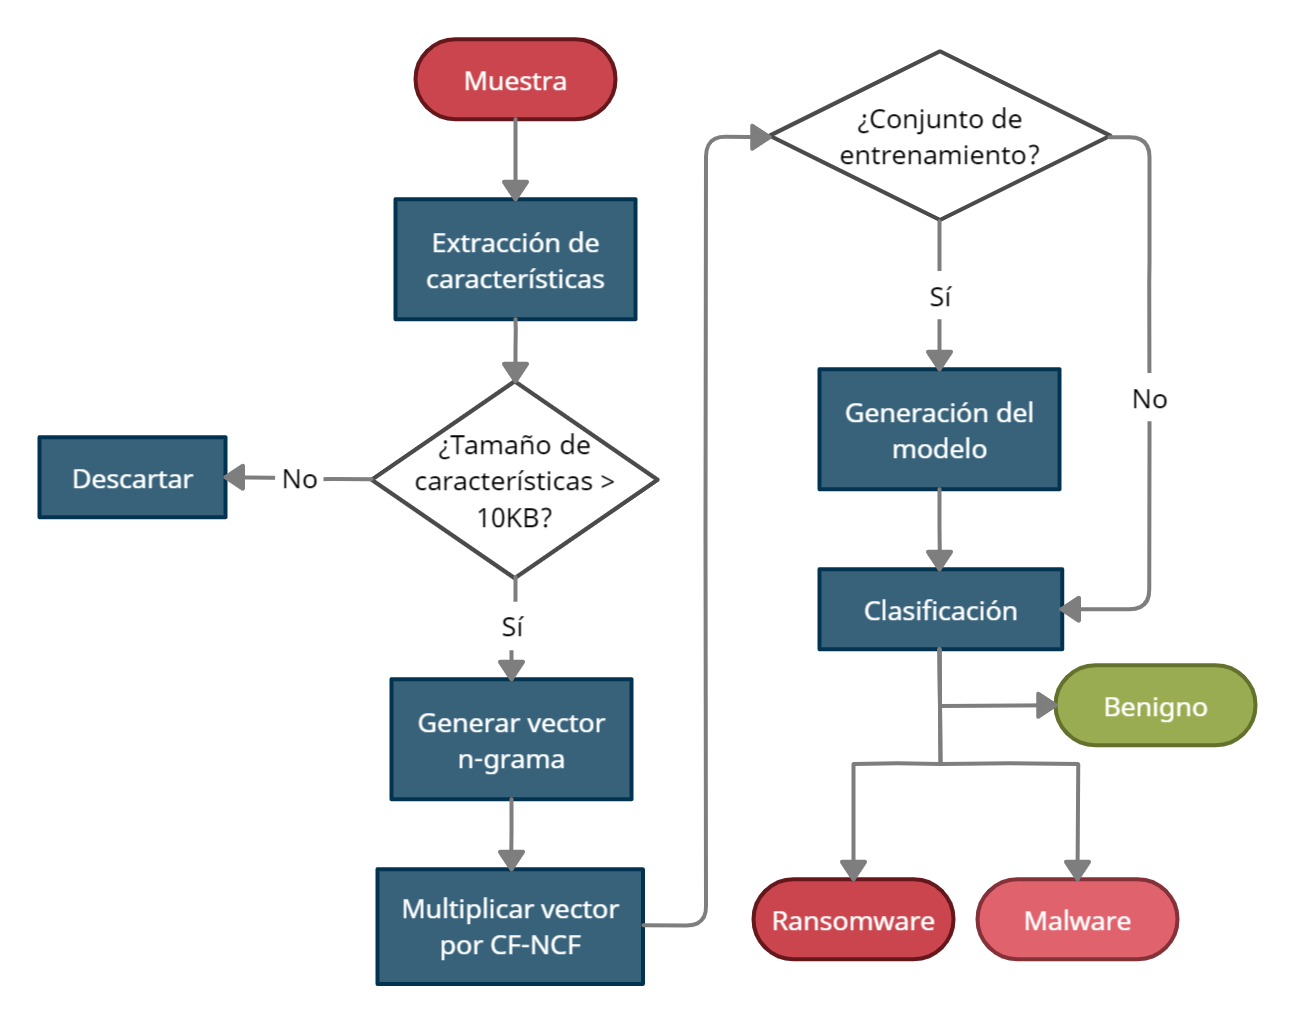
\includegraphics{images/detecting.png}}}
\end{center}
\caption{Diagrama de flujo del sistema propuesto \cite{detecting}}
\label{fig:detecting}
\end{figure}

Mahadevan Supramaniam \textit{et al.} (2019) \cite{Kok2019} proponen un sistema de dos fases que detecta cripto-ransomware antes de que pueda cifrar los archivos del usuario. Las dos fases son:

\begin{itemize}
    \item \textbf{Algoritmo de aprendizaje}: El archivo de muestra se introduce en Cuckoo Sandbox, el cual extrae las llamadas a las \gls{API} de Windows de cifrado (un total de 232). Posteriormente se analizan utilizando un algoritmo de aprendizaje que determina si el programa sospechoso es un cripto-ransomware o no. Este algoritmo selecciona características de forma aleatoria para generar árboles de decisión, ya que hay una gran cantidad de llamadas a las \gls{API} y esto causa \textit{overfitting} o ``sobreajuste''. Si el programa es un cripto-ransomware, el algoritmo genera una firma del programa malicioso y envía una notificación a un repositorio de firmas. 
    
    \item \textbf{Repositorio de firmas}: Una vez que se ha clasificado la muestra, se almacena un la firma de ella utilizando el algoritmo \gls{RSA} en una base de datos \gls{SQL}. La finalidad es que, cuando se vaya a ejecutar un archivo, primero se compruebe en la base de datos, de forma más rápida y eficiente, mediante consultas \gls{SQL}. Tener este repositorio permite la detección de las amenazas en una etapa mucho más temprana, aunque solo puede detectar cripto-ransomware conocido.
\end{itemize}

Las dos fases de este sistema, el cual está representado en la Figura \ref{fig:peda}, forman dos capas de detección temprana para cripto-ransomware, garantizando al usuario que no va a perder ningún archivo. En este trabajo se centran en la primera fase, desarrollando un algoritmo de aprendizaje al que llaman PEDA, obteniendo una \gls{TPR} del 98,72\%, un \gls{AUC} del 99,3\% y una tasa de falsos positivos (\gls{FPR}) un 1,56\% más baja en comparación con los algoritmos \gls{NB}, \gls{RF}, una mezcla de los dos anteriores (método de ensemble) y con el algoritmo EldeRan desarrollado en \cite{elderan}. Usan un \textit{dataset} extraído por el \gls{RISS} en 2016, que contiene datos de \gls{API} de 10 familias de ransomware y de software benigno, en concreto 582 muestras de ransomware y 942 de software benigno.


\begin{figure}[h!]
\begin{center}
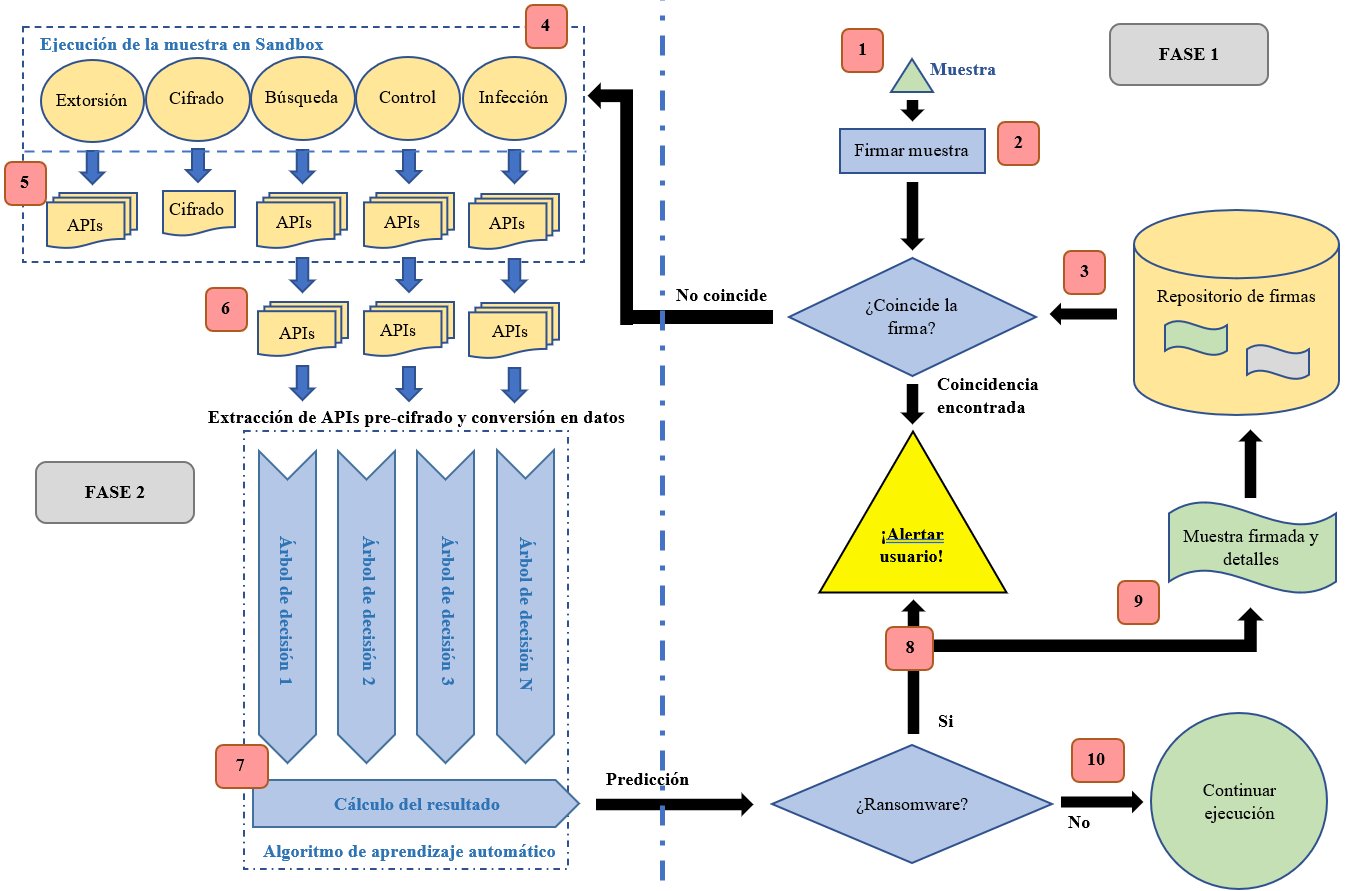
\includegraphics[width=1\linewidth]{images/peda.PNG}
\end{center}
\caption{Modelo del sistema propuesto por \cite{Kok2019}}
\label{fig:peda}
\end{figure}

\newpage

Brijesh Jethva \textit{et al.} (2019) \cite{entropy} propone un sistema de detección de ransomware dinámico mediante la combinación de un modelo de aprendizaje automático con modelos de entropía y firmas de archivos. Con este nuevo enfoque, se observa que el objetivo del ransomware son áreas específicas de claves de registro y su ejecución implica operaciones de alta entropía en extensiones de archivo desconocidas. Las características más seleccionadas son las llamadas a la \gls{API} y las claves de las operaciones de registro, pero la presencia de otras características como las bibliotecas de enlaces dinámicos (\gls{DLL}), los directorios accedidos, las líneas de comando, cadenas insertadas, etc. Con todas estas características, se seleccionan las más importantes con la ayuda de métodos de selección de características para evitar el \textit{overfitting} o sobreajuste para posteriormente clasificarlas mediante técnicas de aprendizaje automático, que son \gls{SVM}, \gls{LR} y \gls{RF}. Para realizar el estudio, utilizan un conjunto de datos que consta de 666 muestras de ransomware y 103 archivos benignos. Para balancear estos datos, usan la técnica \gls{SMOTE}, la cual utiliza el algoritmo \gls{KNN} para generar datos nuevos para las clases con menos muestras. En este caso, se generan datos para ambas clases, obteniendo 1.072 muestras de cada una. En los experimentos, el algoritmo que mejor rendimiento tiene es el de \gls{LR}, obteniendo una \gls{TPR} del 100\%, una precisión (\textit{accuracy}) del 98,7\% y una tasa de falsos positivos del 1,41\%.


Jinsoo Hwang \textit{et al.} (2020) \cite{two} proponen un modelo de detección de ransomware con dos etapas. La primera etapa es un modelo de Markov constituido por dos cadenas de Markov, una para ransomware y la otra para programas benignos. Una cadena de Markov se crea con un espacio de estados y una matriz de probabilidades de transición. El espacio de estado abarca todas las llamadas a la \gls{API} de Windows realizadas tanto por las muestras de ransomware como por las de \textit{goodware}. Estas cadenas se utilizan para decidir si la muestra entrante es ransomware o no, comparando las probabilidades de que una muestra pertenezca a cada clase. La segunda etapa consiste en un modelo de aprendizaje automático, usando \gls{RF} para controlar la tasa de falsos negativos (\gls{FNR}) que devuelve el modelo de Markov, ya que es bastante alta (20\%). Para los experimentos, recopilan 1909 muestras de ransomware de VirusShare y 1139 muestras de \textit{goodware} de Softonic, ejecutándolas dentro de Cuckoo Sandbox para obtener los reportes de donde extraen la secuencia de llamadas a las \gls{API}. Al final de las dos etapas, obtienen una precisión (\textit{accuracy}) del 97,3\%, una tasa de falsos positivos (\gls{FPR}) del 4,8\% y una tasa de falsos negativos (\gls{FNR}) del 1,5\%.


S.H. Kok \textit{et al.} (2020) \cite{Kok2020} proponen un sistema que detecte cripto-ransomware antes de que entre en la etapa de cifrado de archivos (\gls{PEDA}). \gls{PEDA} proporciona dos niveles de detección: el primer nivel consiste en una comparación de firmas, generadas con \gls{SHA}-256. Se compara la firma del archivo sospechoso con firmas de diferentes tipos de ransomware conocidos almacenadas en un repositorio MySQL. Si coinciden los \textit{hashes}, se alerta al usuario de que el archivo es un ransomware. Si no, \gls{PEDA} entra en la segunda etapa, que consiste en enviar ese archivo a Cuckoo Sandbox para que lo analice y obtenga el reporte de su comportamiento. De ese reporte se extraen las \gls{API} que se llaman antes de que empiece el proceso de cifrado, por lo que el algoritmo sacará todas las \gls{API} hasta que encuentre una que empiece por ``crypt''. Se identifican 14 \gls{API}s importantes para diferenciar entre ransomware y goodware, con 3 de ellas encontradas en la mayor parte de ransomwares. Posteriormente las \gls{API} extraídas (232 en total) se guardarán en un archivo de valores separados por comas (\gls{CSV}), el cual se introducirá en el algoritmo de aprendizaje automático \gls{RF} para que prediga si el archivo sospechoso es un ransomware o no. Si la predicción lo identifica como ransomware, \gls{PEDA} pondrá en cuarentena el archivo, alertará al usuario y almacenará su firma en el repositorio MySQL de firmas. La Figura \ref{fig:peda2} muestra el flujo de datos del sistema \gls{PEDA}. Para entrenar el modelo de \gls{ML}, utilizan tres \textit{datasets} con un total de 942 muestras de \textit{goodware} y 1691 muestras de ransomware de VirusShare y theZoo. El modelo obtiene una exhaustividad (\textit{recall}) del 99,9\% con validación cruzada de 10 iteraciones en dos de las tres \textit{datasets}, usando un ratio de entrenamiento:prueba 80:20. En cuanto a las limitaciones, \gls{PEDA} tiene una importante dependencia de uso de las \gls{API}s de Windows, lo que supone que no sería capaz de detectar ransomware que utilice su propio código nativo de cifrado, lo que convierte este algoritmo en un suplemento para la detección de ransomware y no un sistema completo para ello.

\begin{figure}[htb]
\begin{center}
\includegraphics[width=1\linewidth]{images/peda2.PNG}
\end{center}
\caption{Representación del flujo de datos del sistema PEDA propuesto por S.H. Kok \textit{et al.} \cite{Kok2020}}
\label{fig:peda2}
\end{figure}

La detección basada en el análisis del comportamiento se basa en identificar cambios relevantes en el sistema. Abdullahi Arabo \textit{et al.} en \cite{ARABO2020289} (2020) desarrollaron un programa que recopila del sistema las llamadas a \gls{DLL} de \gls{API}, el uso de los recursos del sistema, y los archivos utilizados por  los procesos. Dicha información se discretiza y posteriormente toma dos caminos: a una solución de \gls{ML}, utilizando árboles de decisión, \gls{RF} y redes neuronales, que será capaz de detectar ransomware después del suficiente entrenamiento, y a un sistema de detección mediante umbrales, debido a que no cualquier tipo de datos, como las cadenas, pueden ser introducidos a una solución de \gls{ML}.

La detección del ransomware se lleva a cabo mediante un \textit{script} de Python. Se ejecutan ataques ransomware en una máquina virtual Windows 7, que destruirían dicho \textit{script} con la información que ha recopilado, así que, dicha máquina está conectada con otra base Linux mediante un canal seguro para el paso de la información. Se crean dos hilos principales diferenciados porque hay datos que no tardan el mismo tiempo en ser obtenidos: Hilo ``analysis'', que recoge datos variables en bucle hasta el final del proceso y el  Hilo ``info'', el cual recoge datos constantes, los manda y finaliza.También existen otros tres para leer el nombre de los ficheros,y reconocer su extensión, puesto que los datos cifrados de forma maligna adaptan extensiones reconocibles(p.e.: .wncry), los \textit{tagfiles} y para los datos que son muy lentos de obtener. Se utiliza también el programa Tiny tracer: cuando se ejecuta un programa con él, genera un archivo con todas las llamadas a \gls{DLL} de \gls{API}.

Se crea un sistema basado en media de pesos para reconocer si un dato detecta el ransomware o no. Los datos son procesados por funciones, que tienen un cierto umbral: si lo sobrepasan devolverán 1, por el contrario 0, y se compara con un coeficiente, que depende del umbral y la función. Al final, todos estos valores se utilizan para elaborar una media. Si es por encima de 0,5 es sospechoso de ser malicioso y salta un pop-up al usuario para permitir matar al proceso.

Sana Aurangzeb \textit{et al.} (2021) \cite{Aurangzeb2021} exponen un trabajo basado principalmente en el análisis dinámico enfocado a los \gls{HPC}, que son variables propias de la actividad del hardware como por ejemplo ciclos de reloj, accesos a caché, fallos de caché, instrucciones de salto tomadas, etc. En este estudio se utilizan 11 variables \gls{HPC} para la clasificación de ransomware, que se hará entre ransomware y non-ransomware, siendo non-ransomware muestras de malware y no de goodware. Esto se debe ya que se el ransomware está considerado uno de los tipos de malware que mayor daño provocan en términos financieros. 
A la hora de construir el \textit{dataset}, se obtienen 160 muestras de malware de VirusShare y tras un análisis estático en la misma plataforma se etiquetan como ransomware o non-ransomware. Una vez obtenidas las muestras, se ejecutan en un entorno seguro y se recoge la información relativa a los \gls{HPC}. Para asegurar la precisión y corrección de los datos se ejecuta cada muestra tres veces en una máquina virtual. Los 11 \gls{HPC} recogidos para entrenar el modelo son \textit{task clock}, \textit{context switching}, \textit{\gls{CPU} utilized}, \textit{\gls{CPU} migrations}, \textit{page faults}, \textit{\gls{CPU} cycles}, \textit{cache-misses}, \textit{instruction retires}, \textit{branch taken}, \textit{branch-misses} y \textit{execution time}. Con estas variables se construye una matriz de correlación para seleccionar los atributos concretos a utilizar y así ahorrar costes computacionales.
Para el entrenamiento de los datos se utiliza un 80\% del \textit{dataset} y el resto son usados para prueba. Además, se utiliza el método \textit{k-fold cross-validation}.
En la Figura \ref{fig:im13} se puede ver el flujo del proceso de entrenamiento y prueba.
Se utilizan cuatro modelos de clasificación, árboles de decisión (ofrece una precisión de 0,94), bosques aleatorios (precisión de 0,97), potenciación de gradiente (precisión de 0,94) y potenciación extrema de gradiente (ofrece una precisión de 0,97).
Las conclusiones obtenidas de este estudio es que existe la posibilidad de explotar características hardware para la detección de ransomware. Por otro lado, como no se trabaja con muestras benignas, se desconoce el comportamiento que tendrá el uso de estas características para detectar ransomware, además, la recogida de características es específica de un sistema con una configuración hardware determinada, lo que implica que si el sistema en el que se recogen los datos tiene otra arquitectura, el modelo no será aplicable.

\begin{figure}[htb]
\begin{center}
\includegraphics[width=1\linewidth]{images/hpc.PNG}
\end{center}
\caption{Flujo del proceso de entrenamiento y prueba.}
\label{fig:im13}
\end{figure}


A continuación se muestra una Tabla \ref{tab:estadoarte} comparativa de los trabajos previamente mencionados que usan la extracción de \gls{API}s para la detección de malware y ransomware, exponiendo de manera clara qué algoritmos de aprendizaje automático utilizan, qué datos usan y qué resultados obtienen:

{\footnotesize
\begin{longtable}{|p{0.11\textwidth}|p{0.13\textwidth}|p{0.3\textwidth}|p{0.35\textwidth}|}
\caption{Tabla comparativa de los trabajos que usan aprendizaje automático para detectar malware mediante la extracción de APIs.}
\label{tab:estadoarte}
\\
\hline
\rowcolor[HTML]{C0C0C0} 
\multicolumn{1}{|c|}{\cellcolor[HTML]{C0C0C0}{\color[HTML]{000000} \textbf{Trabajo}}} &
\multicolumn{1}{c|}{\cellcolor[HTML]{C0C0C0}{\color[HTML]{000000} \textbf{Algoritmos}}} &
\multicolumn{1}{c|}{\cellcolor[HTML]{C0C0C0}{\color[HTML]{000000} \textbf{Conjuntos de datos}}} &
\multicolumn{1}{c|}{\cellcolor[HTML]{C0C0C0}{\color[HTML]{000000} \textbf{Resultados}}} \\ \hline
\endfirsthead

\hline
\rowcolor[HTML]{C0C0C0} 
\multicolumn{1}{|c|}{\cellcolor[HTML]{C0C0C0}{\color[HTML]{000000} \textbf{Trabajo}}} &
\multicolumn{1}{c|}{\cellcolor[HTML]{C0C0C0}{\color[HTML]{000000} \textbf{Algoritmos}}} &
\multicolumn{1}{c|}{\cellcolor[HTML]{C0C0C0}{\color[HTML]{000000} \textbf{Conjuntos de datos}}} &
\multicolumn{1}{c|}{\cellcolor[HTML]{C0C0C0}{\color[HTML]{000000} \textbf{Resultados}}} \\ \hline
\endhead

\cite{automatic} (2011)    &
  - Hierarchical clustering (agrupamiento jerárquico) \newline - Nearest prototype classifier &
  - 3.133 muestras de clases conocidas de malware de CWSandbox \newline - 33.698 muestras de clases desconocidas de malware de Sunbelt Software &
  - Precisión: 99,6\% \newline - Valor-F: 95\%. \\ \hline
\cite{zero} (2011)    &
  - \gls{NB} \newline - \gls{KNN} \newline - \gls{DT} \newline - \gls{SVM} &
  - 51.223 muestras de malware del proyecto Honeynet y VX Heaven \newline - 15.480 muestras de goodware &
  - \gls{DT}: \gls{TPR} 93\%, \gls{FPR} 6,8\%, Precisión 93,1\%, Valor-F 93\%, Area \gls{ROC} 93,1\% \newline - \gls{KNN}: \gls{TPR} 94,8\%, \gls{FPR} 5,1\%, Precisión 94,8\%, Valor-F 94,8\%, Area \gls{ROC} 96,6\% \newline - \gls{NB}: \gls{TPR} 91\%, \gls{FPR} 9\%, Precisión 91\%, Valor-F 91\%, Area \gls{ROC} 93,8\% \newline - \gls{SVM} PolyKernel normalizado: \gls{TPR} 98,6\%, \gls{FPR} 2,5\%, Precisión 97,8\%, Valor-F 98,6\%, Area \gls{ROC} 98,2\% \newline - \gls{SVM} PolyKernel: \gls{TPR} 93,4\%, \gls{FPR} 6,9\%, Precisión 93,6\%, Valor-F 93,4\%, Area \gls{ROC} 93,2\% \newline - \gls{SVM} Puk: \gls{TPR} 94\%, \gls{FPR} 6,4\%, Precisión 94\%, Valor-F 93,2\%, Area \gls{ROC} 93,9\% \newline - \gls{SVM} \gls{RBF}: \gls{TPR} 92,9\%, \gls{FPR} 7,3\%, Precisión 92,9\%, Valor-F 92,9\%, Area \gls{ROC} 92,8\% \\ \hline
\cite{ravimalware} (2012)  & 
    - \gls{NB} \newline - \gls{SVM} \newline - \gls{DT} \newline - Algoritmo clasificador propio de 4-gramas & 
    - 179 muestras de malware de VXHeavens \newline - 94 muestras de goodware de una instalación de Windows XP &
    Precisión: \newline - \gls{NB}: 48,69\% \newline - \gls{SVM}: 64,43\% \newline - \gls{DT}: 56,77\% \newline - Algoritmo propuesto: 90\%\\ \hline
\cite{elderan} (2016)      & 
    - \gls{NB} \newline - \gls{SVM} \newline - EldeRan & 
    - 582 muestras de ransomware de 11 familias de VirusShare \newline - 942 muestras de goodware de Software Informer &
    - EldeRan: \gls{AUC} 99,49\%, \gls{FPR} 1,61\%, \gls{TPR} 96,34\% \newline - \gls{SVM}: \gls{AUC} 99,29\%, \gls{FPR} 1,99\%, \gls{TPR} 92,19\% \newline - \gls{NB}: \gls{AUC} 96,96\%, \gls{FPR} 9,58\%, \gls{TPR} 94,53\% \\ \hline
\cite{shallow} (2017)      & 
    - \gls{MLP} \newline - \gls{LR} \newline - \gls{NB} \newline - \gls{DT} \newline - \gls{RF} \newline - \gls{KNN} \newline - \gls{SVM} & 
    - 755  muestras  de  ransomware de varias fuentes \newline -  219 muestras de goodware &
    - \gls{MLP}: Precisión 100\%, Exactitud 100\%, Exhaustividad 100\%, Valor-F 100\% \newline - \gls{LR}: Precisión 98,8\%, Exactitud 98,5\%, Exhaustividad 100\%, Valor-F 99,3\% \newline - \gls{NB}: Precisión 97,2\%, Exactitud 96,6\%, Exhaustividad 100\%, Valor-F 98,3\% \newline - \gls{DT}: Precisión 96,4\%, Exactitud 95,7\%, Exhaustividad 100\%, Valor-F 97,8\% \newline - \gls{RF}: Precisión 98,4\%, Exactitud 98\%, Exhaustividad 100\%, Valor-F 99\% \newline - \gls{KNN}: Precisión 96,8\%, Exactitud 96,2\%, Exhaustividad 100\%, Valor-F 99,3\% \newline - \gls{SVM}: Precisión 98,8\%, Exactitud 98,5\%, Exhaustividad 100\%, Valor-F 99,3\% \\ \hline
\cite{flow} (2017)         & 
    - \gls{NB} \newline - \gls{SVM} \newline - \gls{RF} \newline - \gls{LR} & 
    - 83 muestras de ransomware diferentes de VirusShare \newline - 85 muestras de goodware de Software Informer &
    - \gls{LR}: Precisión: 98,2\%, \gls{TPR} 97,6\%, \gls{FPR} 1,2\% \newline - \gls{SVM}: Precisión: 95,8\%, \gls{TPR} 96,4\%, \gls{FPR} 4,7\% \newline - \gls{RF}: Precisión: 95,8\%, \gls{TPR} 96,4\%, \gls{FPR} 4,7\% \newline - \gls{NB}: Precisión: 92,3\%, \gls{TPR} 94\%, \gls{FPR} 9,4\% \\ \hline
\cite{detectingSVM} (2018) & 
    - \gls{SVM} & 
    - 276 muestras de ransomware \newline - 312 muestras de goodware &
    - Precisión: 97.48\% \newline - Tasa de error: 1.64\% \\ \hline
\cite{detecting} (2019)    & 
    - \gls{RF} \newline - \gls{LR} \newline - \gls{NB} \newline - \gls{SGD} \newline - \gls{KNN} \newline - \gls{SVM} & 
    - 1000 muestras de ransomware \newline - 900 muestras de malware \newline - 300 muestras de goodware &
    - \gls{RF}: Precisión 98,39\%, Exhaustividad 98,55\%, Valor-F 98,56\%, Exactitud 98,58\% \newline - \gls{KNN}: Precisión 96,13\%, Exhaustividad 96,13\%, Valor-F 96,25\%, Exactitud 95,50\% \newline - \gls{NB}: Precisión 87,43\%, Exhaustividad 87,92\%, Valor-F 82,72\%, Exactitud 89,38\% \newline - \gls{SGD}: Precisión 93,96\%, Exhaustividad 90,95\%, Valor-F 90,22\%, Exactitud 91,61\% \newline - \gls{LR}: Precisión 90,08\%, Exhaustividad 93,99\%, Valor-F 92,98\%, Exactitud 92,07\% \newline - \gls{SVM}: Precisión 74,81\%, Exhaustividad 78,99\%, Valor-F 75,98\%, Exactitud 79,95\% \\ \hline
\cite{Kok2019} (2019)         & 
    - \gls{PEDA} \newline - \gls{RF} \newline - \gls{NB} \newline - Ensamble (\gls{RF}+\gls{NB}) & 
    - 582 muestras de ransomware \newline - 942 muestras de goodware \newline Los dos conjuntos de muestras fueron extraídos por el \gls{RISS} &
    - \gls{PEDA}: \gls{AUC} 99,30\%, \gls{FPR} 1,56\%, Precisión 97,05\%, \gls{TPR} 95\% \newline - \gls{RF}: \gls{AUC} 95\%, \gls{FPR} 7\%, Precisión 92\%, \gls{TPR} 91\% \newline - \gls{NB}: \gls{AUC} 81\%, \gls{FPR} 15\%, Precisión 83\%, \gls{TPR} 79\% \newline - Ensamble: \gls{AUC} 82,5\%, \gls{FPR} 16\%, Precisión 88\%, \gls{TPR} 98\% \\ \hline
\cite{entropy} (2019)      & 
    - \gls{SVM} \newline - \gls{RF} \newline - \gls{LR} & 
    Inicialmente: \newline - 666 muestras de ransomware \newline - 103 muestras de goodware \newline Para balancear los datos, usan \gls{SMOTE} y obtienen 1.072 muestras de cada clase &
    - \gls{SVM}: Precisión 98\%, Exhaustividad 97\%, Valor-F 97\% \newline - \gls{RF}: Precisión 97\%, Exhaustividad 97\%, Valor-F 97\% \newline - \gls{LR}: Precisión 97\%, Exhaustividad 97\%, Valor-F 97\% \newline \\ \hline
\cite{two} (2020)          & 
    - \gls{RF} & 
    - 1909 muestras de ransomware de VirusShare \newline - 1139 muestras de goodware de Softonic &
    - Precisión: 97,3\% \newline - \gls{FPR}: 4,8\% \newline - \gls{FNR}: 1,5\% \newline - Valor-F: 97,0\% \\ \hline
\cite{Kok2020} (2020)        & 
    - \gls{PEDA} (\gls{RF} discretizado) \newline - \gls{RF} & 
    Tres datasets: \newline - Dataset PE (con ransomware criptográfico): \newline 942 muestras de goodware \newline 205 muestras de cripto-ransomware \newline - Dataset Old (creada en 2016): \newline 942 muestras de goodware \newline 582 muestras de ransomware \newline - Dataset Full (PE + Old + nuevas muestras de VirusShare y theZoo ): \newline 942 muestras de goodware \newline 904 muestras de ransomware 
    \newline Tras obtener dicho dataset y realizar mediante el algoritmo de este estudio una limpieza de los datos para eliminar repetidos, el dataset restante obtenido es de 912 muestras &
    - Dataset PE: \newline \gls{PEDA}: \gls{TPR} 99,8\%, Precisión 99,9\%, Valor-F 99,9\%, \gls{ROC} 99,9\% \newline \gls{RF}: \gls{TPR} 99,6\%, Precisión 99,6\%, Valor-F 99,4\%, \gls{ROC} 99,5\% \newline - Dataset Old: \newline \gls{PEDA}: \gls{TPR} 95,6\%, Precisión 95,8\%, Valor-F 95,6\%, \gls{ROC} 98,5\% \newline \gls{RF}: \gls{TPR} 95,2\%, Precisión 95,2\%, Valor-F 95,2\%, \gls{ROC} 97,0\% \newline - Dataset Full: \newline \gls{PEDA}: \gls{TPR} 99,6\%, Precisión 99,6\%, Valor-F 99,4\%, \gls{ROC} 99,6\% \newline \gls{RF}: \gls{TPR} 99,7\%, Precisión 99,7\%, Valor-F 99,5\%, \gls{ROC} 99,5\% \\ \hline
\cite{ARABO2020289} (2020) & 
- \gls{NN} \newline
- \gls{KNN} \newline
- \gls{SVM} lineal\newline
- \gls{SVM} \gls{RBF} \newline 
- \gls{GP} \newline
- \gls{DT} \newline
- \gls{RF} \newline
- AdaBoost \newline
- \gls{QDA} \newline
- \gls{NB} &
- 41 aplicaciones benignas \newline
- 34 procesos malware, includios 7 muestras de ransomware &
Precisión: \newline
- \gls{NN}: 52,85\% \newline
- \gls{KNN}: 57,06\% \newline
- \gls{SVM} lineal: 63,05\% \newline
- \gls{SVM} \gls{RBF}: 60,50\%\newline 
- \gls{GP}: 59,8\% \newline
- \gls{DT}: 70,14\% \newline
- \gls{RF}: 75,01\% \newline
- AdaBoost: 61,64\% \newline
- \gls{QDA}: 62,7\% \newline
- \gls{NB}: 58,55 \%  \\ \hline
\cite{Aurangzeb2021} (2021) &
- \gls{DT} \newline
- \gls{RF} \newline
- Gradient Boosting \newline
- Extreme Gradient Boosting \newline&
 160 muestras de las cuales pertenecen 80 a ransomware y 80 a otros tipos de malware &
Precisión: \newline
- \gls{DT}: 94,5\% \newline
- \gls{RF}: 97\% \newline
- Gradient Boosting: 94,5\% \newline
- Extreme Gradient Boosting: 97\% \newline
Valor F: \newline
- \gls{DT}: 94\% \newline
- \gls{RF}: 97\% \newline
- Gradient Boosting: 94\% \newline
- Extreme Gradient Boosting: 97\% \newline
\gls{TPR}: \newline
- \gls{DT}: 88\% \newline
- \gls{RF}: 94\% \newline
- Gradient Boosting: 88\% \newline
- Extreme Gradient Boosting: 94\% \newline
\\ \hline


\end{longtable}}



 

\chapter{Técnica de Detección de Ransomware Propuesta}\label{Capitulo5}
\noindent El capitulo incluye información relacionada con las tecnologías utilizadas en el proyecto, el entorno de trabajo y los datos. En la Sección \ref{sec:sistema} se describe el concepto de \gls{API}, una de las fuentes de datos en crudo y la estructura del modelo. A continuación, la Sección \ref{sec:dataset} está destinada al montaje del laboratorio de análisis de muestras \textit{ransomware}. La Sección \ref{sec:reports} incluye el proceso de construcción del conjunto de datos final, incluyendo información de la estructura de los reportes obtenidos en el análisis y las pautas seguidas para la limpieza y la extracción de características. Por último, en la Sección \ref{sec:model} se detallan el modelo y los algoritmos utilizados, así como librerías importantes para la construcción del mismo.

\section{Descripción del Sistema Propuesto} \label{sec:sistema}

\noindent El objetivo del sistema propuesto es la detección de ransomware mediante la extracción de las llamadas a la \gls{API} de Windows, utilizando algoritmos supervisados de aprendizaje automático para construir un modelo de clasificación que detecte si un archivo es ransomware o no.



Una \gls{API} (interfaz de programación de aplicaciones) proporciona una abstracción para un problema y especifica cómo los clientes deben interactuar con los componentes software para implementar una solución. Suelen ser distribuidas como librerías software, definiendo bloques de desarrollo reusables que permiten añadir funcionalidades en múltiples aplicaciones \cite{reddy2011api}. 

Microsoft suministra a los desarrolladores de Windows una \gls{API} documentada profesionalmente para facilitar el proceso de creación de una aplicación. Ésta provee todas las funcionalidades básicas y permite el despliegue de entornos ricos e interactivos. De manera análoga, una aplicación de Windows puede ser mapeada y explicada por las llamadas a la {API} que realice, entendiendo así su comportamiento. Por ejemplo, si el proceso llama a la función \textit{WriteFile}, se puede saber que se va a escribir en un fichero del sistema. Si se invoca, por ejemplo a \textit{CryptEncrypt}, la aplicación va a efectuar un cifrado en nuestro sistema de ficheros. Este tipo de llamadas pueden ser muy útiles para la detección de ransomware de cifrado, aunque aplicaciones benignas también lo utilicen. Para este estudio, se han recogido un total de 302 llamadas distintas a la \gls{API} de Windows, realizando una distinción en la recogida de datos: se conforma un \textit{dataset} en el que, de manera binaria, un proceso a invocado a la función de sistema correspondiente, y otro que señala la cantidad de llamadas totales para cada función \cite{10.1145/1654988.1655003}.


Los datos utilizados en el proyecto se han obtenido de dos formas diferentes. Primero, el grupo de investigación GASS \cite{GASS01} proporcionó 21 muestras de \textit{ransomware} para su análisis en un entorno controlado, como se explica en la Sección \ref{sec:lab}. Por otro lado, el grupo GASS \cite{GASS01} ha desarrollado una herramienta con la que se accede a un número elevado de muestras, extrayendo múltiples informes obtenidos de análisis realizados en la página web de Cuckoo Sandbox por usuarios anónimos. De esta forma se obtiene un fichero en formato .json con información de 5435 muestras de \textit{ransomware} y otro fichero con información de 10896 muestras de \textit{goodware} (software benigno). Combinando ambos métodos, es posible componer un conjunto de datos inicial de gran extensión y mayor variedad. El análisis de las muestras y la extracción de las características relevantes se explica con más detalle en la Sección \ref{sec:reports}. Finalmente, los resultados obtenidos del análisis se usarán para entrenar al modelo de \gls{ML}.
La Figura \ref{fig:fase1} muestra el proceso en términos generales.

\begin{figure}[h!]
\begin{center}
\includegraphics[width=1\linewidth]{images/fase1.png}
\end{center}
\caption{Extracción de características y creación del modelo predictivo.}
\label{fig:fase1} 
\end{figure}

A partir del entrenamiento se creará un modelo predictivo que podrá decir si archivo es ransomware o benigno. En la fase de predicción se hace uso del modelo predictivo para sacar inferencias, y este proceso es similar al de entrenamiento, ya que ambos comienzan extrayendo características. Sin embargo, esta vez en lugar de entrenar el modelo usando esas características, se predecirá la naturaleza del archivo desconocido. El desarrollo del modelo y los algoritmos de aprendizaje automático usados se detallan en la Sección \ref{sec:algoritmos}. 
La Figura \ref{fig:fase2} muestra este proceso.

\begin{figure}[h!]
\begin{center}
\includegraphics[width=1\linewidth]{images/fase2.png}
\end{center}
\caption{Clasificación de un archivo con un modelo predictivo.}
\label{fig:fase2} 
\end{figure}


La Figura \ref{fig:sistema} representa el diagrama de flujo del sistema propuesto en este trabajo, siguiendo los pasos detallados a continuación:
\begin{enumerate}
    \item Obtención de muestras ransomware y benignas e información de reportes.
    \item Ejecución y análisis de las muestras en un entorno controlado usando Cuckoo Sandbox.
    \item Unión y limpieza de los datos, extracción de características y \textit{dataset}.
    \item División del \textit{dataset} en datos de entrenamiento y datos de prueba.
    \item Entrenamiento del modelo.
    \item Utilización del modelo.
    \item Salida del modelo y clasificación de la muestra.
    \item Análisis, generación de gráficas y conclusiones.
\end{enumerate}

\begin{figure}[h!]
\begin{center}
\includegraphics[width=1\linewidth]{images/sistemapropuesto.PNG}
\end{center}
\caption{Diagrama de flujo del sistema propuesto.}
\label{fig:sistema} 
\end{figure}



\section{Entorno de Obtención de Datos} \label{sec:dataset}

\noindent A la hora de ejecutar muestras reales de \textit{ransomware} para su análisis, se puede causar daño al sistema con borrado de archivos, cambios en los registros y robo de información confidencial, entre otras cosas. Para evitar esto, es preciso contar con un entorno seguro donde ejecutar el malware sin poner en riesgo los equipos o la red \cite{CMA}.

Cuckoo Sandbox es una herramienta de análisis automatizado de malware de código abierto en Windows, macOS, Linux y Android. Esta herramienta utiliza la tecnología de \textit{sandboxing}, que, en terminología informática, es una técnica que consiste en aislar la ejecución de un programa no fiable o malicioso llevándola a un entorno seguro que no comprometa el sistema, de forma que se puedan analizar las actividades del malware sin preocupación por los cambios que realice el proceso maligno.

Existen múltiples herramientas que utilicen \textit{sandboxing} y permitan construir un laboratorio de análisis de malware, entre ellas, Buster Sandbox Analyzer, Zero Wine o Malheur, pero en este trabajo se recurre a Cuckoo Sandbox debido a que es la más completa y, siendo de código abierto y teniendo un diseño modular, permite personalizar cualquier aspecto del procesamiento del análisis de los resultados, de la generación de informes y del entorno de análisis. Además, tiene una guía detallada de los requisitos para integrar la herramienta con el sistema.

Cuckoo Sandbox, se inició como un proyecto de verano parte del programa Google Summer of Code en 2010, lanzando la primera beta en febrero de 2011. El diseñador y desarrollador de Cuckoo, Claudio Guarnieri, es aún el principal coordinador del proyecto. En marzo de 2012, Cuckoo Sandbox ganó la primera ronda del programa Magnificent7 organizado por Rapid7 (un importante sistema de Gestión de Vulnerabilidades y análisis de \textit{endpoints}, con más  de 20 años de trayectoria). Esta herramienta fue mejorando y obteniendo méritos hasta febrero de 2016, cuando la versión 2.0 fue publicada, siendo esta una versión muy completa y adaptada al uso diario.

La arquitectura de Cuckoo se muestra en la Figura \ref{fig:Diagrama}. Consiste en un software central que maneja la ejecución y el análisis de muestras, en el caso de este proyecto, ejecutando cada una en una máquina virtual aislada. De esta forma, los componentes principales de la infraestructura del laboratorio de análisis de malware (y por lo tanto de Cuckoo Sandbox) son una máquina anfitrión que gestiona el proceso de análisis, la cual tendrá acceso a Internet, y un número de máquinas virtuales conectadas a una red virtual donde las muestras de malware se ejecutan de forma segura y aislada para ser analizadas.

\begin{figure}[!htb]
\begin{center}
\includegraphics[width=0.9\linewidth]{images/infraestructuracuckoo.png}
\end{center}
\caption{Arquitectura de Cuckoo Sandbox}
\label{fig:Diagrama}
\end{figure}

Hay otra manera de utilizar Cuckoo Sandbox sin necesidad de una máquina virtual propia, y es mediante el uso de la interfaz web de la herramienta (\href{https://cuckoo.cert.ee/}{Cuckoo Sandbox Online}). La ventaja de este método es que no es necesario construir un laboratorio de análisis con Cuckoo descargado, ya que es accesible mediante Internet. Pero tiene un gran inconveniente, y es la lentitud del análisis, ya que es necesario subir los archivos manualmente uno por uno y si la página web tiene mucha afluencia, el análisis tardará más. Por esta razón se decidió construir un laboratorio de análisis propio en una máquina con el sistema operativo recomendado por los autores de Cuckoo Sandbox, que es Linux con distribución Ubuntu 18.04.5 \gls{LTS}.

\subsection{Laboratorio de análisis} \label{sec:lab}
%anexo a
\label{anexo-a}
\noindent Una vez entendido el concepto de \textit{sandboxing}, y la necesidad de construir un laboratorio de análisis de malware para el trabajo, comienza la preparación del mismo.

La máquina anfitrión será un ordenador con sistema operativo Linux, utilizando la distribución Ubuntu en la versión 18.04.5 \gls{LTS}.

Se necesitan una serie de requisitos para la instalación y el correcto funcionamiento de Cuckoo.

Será necesario tener la versión adecuada de Python (actualmente soporta Python 2.7) e instalar una serie de bibliotecas:

\begin{listing}[style=consola, numbers=none]
$ sudo apt-get install python python-pip python-dev libffi-dev libssl-dev
$ sudo apt-get install python-virtualenv python-setuptools
$ sudo apt-get install libjpeg-dev zlib1g-dev swig
\end{listing}

Para poder utilizar la interfaz web Django y PostgreSQL como base de datos, se necesita MongoDB y PostgreSQL:

\begin{listing}[style=consola, numbers=none]
$ sudo apt-get install mongodb
$ sudo apt-get install postgresql libpq-dev
\end{listing}

Las máquinas virtuales basadas en Windows 7 donde se ejecutarán las muestras de malware serán generadas a través de VirtualBox, un software de virtualización muy completo el cual está soportado por Cuckoo, aunque se puede utilizar otro software de virtualización. En este caso se utiliza la versión 5.2.42 de VirtualBox, la cual se puede descargar e instalar desde la página oficial o utilizando los comandos siguientes:

\begin{listing}[style=consola, numbers=none]
$ echo deb http://download.virtualbox.org/virtualbox/debian xenial contrib | sudo \
tee -a /etc/apt/sources.list.d/virtualbox.list
$ wget -q https://www.virtualbox.org/download/oracle_vbox_2016.asc -O- | sudo \
apt-key add -
$ sudo apt-get update
$ sudo apt-get install virtualbox-5.2
\end{listing}

Para poder obtener información de la actividad de red del malware se recurre a tcpdump, que rastreará la red para capturar el tráfico a la hora de analizar una muestra.

\begin{listing}[style=consola, numbers=none]
$ sudo apt-get install tcpdump apparmor-utils
\end{listing}

Esta herramienta necesita privilegios de superusuario, los cuales les serán otorgados únicamente a ella y no a Cuckoo Sandbox:

\begin{listing}[style=consola, numbers=none]
$ sudo groupadd pcap

$ sudo usermod -a -G pcap (nombre_usuario)
$ sudo chgrp pcap /usr/sbin/tcpdump
$ sudo setcap cap_net_raw,cap_net_admin=eip /usr/sbin/tcpdump
$ sudo aa-disable /usr/sbin/tcpdump
\end{listing}

Tras esto, se instala M2crypto, un módulo de Python que será necesario para el análisis de muestras:

\begin{listing}[style=consola, numbers=none]
$ sudo pip install m2crypto
\end{listing}

En este caso, se utiliza VirtualBox y será necesario incluir al usuario con el que se ejecuta Cuckoo en el grupo ``vboxusers'', para que Cuckoo pueda identificar las máquinas virtuales:

\begin{listing}[style=consola, numbers=none]
$ sudo usermod -a -G vboxusers (nombre_usuario)
\end{listing}

A continuación, se crea un entorno virtual, para añadir otro factor más de seguridad al laboratorio y en este entorno será donde posteriormente se instale Cuckoo Sandbox y se trabaje. Para ello, descargamos un \href{https://gist.github.com/jstrosch/de20131dda2aac5cd1116dd44b8f2474#file-cuckoo-setup-virtualenv-sh}{\textcolor{blue}{script bash de GitHub}} el cual sirve para instalar esta funcionalidad: 

\begin{listing}[style=consola, numbers=none]
$ sudo -u <USERNAME> cuckoo-setup-virtualenv.sh
\end{listing}

Una vez instalada esta herramienta, se crea un entorno virtual, en el caso de este trabajo se le ha dado el nombre de ``cuckoo-test'' y llegados a este punto, siempre se trabajará dentro de este entorno, por lo que será muy importante asegurarse de que estamos dentro del entorno virtual al utilizar un terminal.


\begin{listing}[style=consola, numbers=none]
$ mkvirtualenv -p python2.7 cuckoo-test
\end{listing}

Tras la ejecución del comando anterior, se estará trabajando dentro de un entorno virtual donde se realizan el resto de pasos. Primero se requiere la actualización de los módulos pip y setuptools y después, se procede a la instalación de Cuckoo:

\begin{listing}[style=consola, numbers=none]
(cuckoo-test) $ pip install -U pip setuptools
(cuckoo-test) $ pip install -U cuckoo
\end{listing}

A continuación, se deberá descargar una ISO de Windows 7 y se monta: \cite{HATCHING}

\begin{listing}[style=consola, numbers=none]
(cuckoo-test) $ wget https://cuckoo.sh/win7ultimate.iso
(cuckoo-test) $ mkdir /mnt/win7
(cuckoo-test) $ sudo mount -o ro,loop win7ultimate.iso /mnt/win7
\end{listing}

Para gestionar la creación de máquinas virtuales para Cuckoo, el software que usan y la captura de estados, el uso de la herramienta VMCloak facilitará estas tareas ya que está diseñada para crear máquinas virtuales que Cuckoo Sandbox pueda utilizar. \cite{VMCLOAK} Es necesario instalar algunos paquetes previos para la correcta integración con Cuckoo, y después instalar VMCloak: \cite{HATCHING}

\begin{listing}[style=consola, numbers=none]
(cuckoo-test) $sudo apt-get -y install build-essential libssl-dev libffi-dev \ 
python-dev genisoimage
(cuckoo-test) $ sudo apt-get -y install zlib1g-dev libjpeg-dev
(cuckoo-test) $ sudo apt-get -y install python-pip python-virtualenv \ 
python-setuptools swig

(cuckoo-test) $ pip install -U vmcloak
\end{listing}

Una vez la herramienta está instalada, se crea una interfaz de red a la que se conectarán las máquinas virtuales, se configura la ISO montada previamente con las características adecuadas (en este caso, serán máquinas virtuales con 2 CPUs y una memoria RAM de 2048MB) utilizando los siguientes comandos: \cite{HATCHING}

\begin{listing}[style=consola, numbers=none]
(cuckoo-test) $ vmcloak-vboxnet0 
(cuckoo-test) $ vmcloak init --verbose --win7x64 win7x64base --cpus 2 --ramsize 2048
\end{listing}

El siguiente paso es instalar el software necesario, que una vez creados los estados de la imagen, no se podrá modificar, por eso, el primer paso será clonar la máquina en su versión original vacía, para instalar software ahí y guardar los estados. 
Entre el software que necesario para las máquinas encontramos java, adobepdf, flash y pillow (este último será el paquete que realice capturas de pantalla durante el análisis del malware): \cite{HATCHING}

\begin{listing}[style=consola, numbers=none]
(cuckoo-test) $ vmcloak clone win7x64base cuckooVM
(cuckoo-test) $ vmcloak install cuckooVM adobepdf dotnet java flash vcredist \ 
vcredist.version=2015u3 wallpaper
(cuckoo-test) $ vmcloak install cuckooVM pillow
\end{listing}

Llegados a este punto, se crean los estados de la máquina virtual. Dadas las características del equipo en el que se está construyendo el laboratorio de análisis de malware, se crean 3 estados, lo que permitirá realizar un máximo de 3 análisis simultáneos. Con el siguiente comando, se crearán 3 máquinas virtuales con IPs 192.168.56.101, 192.168.56.102 y 192.168.56.103: \cite{HATCHING}

\begin{listing}[style=consola, numbers=none]
(cuckoo-test) $ vmcloak snapshot --count 3 cuckooVM 192.168.56.101
\end{listing}

Con todo lo realizado hasta ahora, el laboratorio está casi preparado y únicamente quedaría configurar Cuckoo Sandbox para ponerlo a funcionar. Para ello es necesario iniciar cuckoo, que mostrará por defecto el directorio de trabajo ``\verb!/home/nombre_usuario/.cuckoo!'', este directorio se podrá modificar sin problema, aunque en el caso de este proyecto, se trabajará en el definido por defecto. 

\begin{listing}[style=consola, numbers=none]
(cuckoo-test) $ cuckoo init
(cuckoo-test) $ cuckoo community
\end{listing}

También será necesario modificar los ficheros de configuración de Cuckoo, que se encuentran en la carpeta ``\verb!conf!'' dentro del directorio principal de trabajo, personalizando los ajustes y configurando las máquinas virtuales.

En primer lugar, la edición del fichero ``\verb!virtualbox.conf!'' que contiene opciones sobre el software de virtualización, en este caso, se edita el campo ``\verb!mode!'' que por defecto tendrá el valor ``\verb!headless!'' y pone el valor ``\verb!gui!''. Este cambio permitirá ver la máquina virtual en ejecución cuando se realice un análisis, si por el contrario se quiere ver únicamente el resultado final y no lo que va sucediendo, se mantendrá el valor ``\verb!headless!''. El fichero quedaría de la siguiente manera:

\lstset{language=bash,breaklines=true, basicstyle=\footnotesize}
\begin{lstlisting}[frame=single, caption=Fichero ``virtualbox.conf'']
[virtualbox]
# Specify which VirtualBox mode you want to run your machines on.
# Can be "gui" or "headless". Please refer to VirtualBox's official
# documentation to understand the differences.
mode = gui
\end{lstlisting}

Con el siguiente comando, que modificará el fichero anterior, se añaden las máquinas virtuales creadas a Cuckoo con su configuración. \cite{HATCHING}

\begin{listing}[style=consola, numbers=none]
(cuckoo-test) $ while read -r vm ip; do cuckoo machine --add $vm $ip; 
done < <(vmcloak list vms)
\end{listing}

El resultado del fichero será el siguiente:

\break

\lstset{language=bash,breaklines=true, basicstyle=\footnotesize}
\begin{lstlisting}[frame=single, caption=Fichero ``virtualbox.conf'', breaklines=true]
[192.168.56.1011]
# Specify the label name of the current machine as specified in your
# VirtualBox configuration.
label = 192.168.56.1011

# Specify the operating system platform used by current machine
# [windows/darwin/linux].
platform = windows

# Specify the IP address of the current virtual machine. Make sure that the
# IP address is valid and that the host machine is able to reach it. If not,
# the analysis will fail.
ip = 192.168.56.101

# (Optional) Specify the snapshot name to use. If you do not specify a
# snapshot name, the VirtualBox MachineManager will use the current snapshot
# Example (Snapshot1 is the snapshot name):
snapshot = 

# (Optional) Specify the name of the network interface that should be used
# when dumping network traffic from this machine with tcpdump. If specified,
# overrides the default interface specified in auxiliary.conf
# Example (vboxnet0 is the interface name):
interface = 

# (Optional) Specify the IP of the Result Server, as your virtual machine 
# sees it.
# The Result Server will always bind to the address and port specified in
# cuckoo.conf, however you could set up your virtual network to use NAT/PAT,
# so you can specify here the IP address for the Result Server as your 
# machine sees it. If you don't specify an address here, the machine will 
# use the default value from cuckoo.conf.
# NOTE: if you set this option you have to set result server IP to 0.0.0.0 
# in cuckoo.conf.
# Example:
resultserver_ip = 192.168.56.1
# (Optional) Specify the port for the Result Server, as your virtual machine
# sees it. The Result Server will always bind to the address and port 
# specified in cuckoo.conf, however you could set up your virtual network 
# to use NAT/PAT, so you can specify here the port for the Result Server as 
# your machine sees it. If you don't specify a port here, the machine will 
# use the default value from cuckoo.conf.
# Example:
resultserver_port = 0
# (Optional) Set your own tags. These are comma separated and help to
# identify specific VMs. You can run samples on VMs with tag you require.
tags = 
# Mostly unused for now. Please don't fill it out.
options = 
# (Optional) Specify the OS profile to be used by volatility for this
# virtual machine. This will override the guest_profile variable in
# memory.conf which solves the problem of having multiple types of VMs
# and properly determining which profile to use.
osprofile = 

[192.168.56.1012]
.
.
. 
\end{lstlisting}

Hecho esto, se quiere dar acceso a Internet a las máquinas de análisis y para ello, es necesario activar la redirección de paquetes (\textit{forwarding}) en la interfaz creada para VirtualBox y en la interfaz de salida (que en este caso es ``wlo1'', pero puede ser ``eth0'' u otra, dependiendo del sistema).

La conexión a Internet es importante para que las muestras de malware muestren su comportamiento completo en los análisis, ya que que se conecten a la red es algo básico en la mayoría de ellas \cite{HATCHING}:

\begin{listing}[style=consola, numbers=none]
(cuckoo-test) $ sudo sysctl -w net.ipv4.conf.vboxnet0.forwarding=1
(cuckoo-test) $ sudo sysctl -w net.ipv4.conf.wlo1.forwarding=1
\end{listing}

Otro aspecto a configurar de Cuckoo, es el módulo ``rooter'', que concede a Cuckoo ciertos permisos para trabajar con comandos de red y poder realizar análisis con opciones de encaminamiento y así sacar el máximo partido a análisis:

\begin{listing}[style=consola, numbers=none]
(cuckoo-test) $ cuckoo rooter --sudo --group gonzalo
\end{listing}

Por último, antes de poder iniciar la interfaz web de Cuckoo Sandbox y empezar a realizar análisis, los últimos ficheros que necesitan edición son el fichero ``\verb!routing.conf!'', cambiando el apartado ``\verb!internet!'' con valor ``\verb!none!'' y dándole el nuevo valor ``\verb!wlo1!'' (la interfaz de red) y el fichero ``\verb!reporting.conf!'' cambiando el valor de ``\verb!enabled!'' en el apartado ``\verb!mongodb!'' de ``\verb!no!'' a ``\verb!yes!'' \cite{HATCHING}.

\lstset{language=bash,breaklines=true, basicstyle=\footnotesize}
\begin{lstlisting}[frame=single, caption=Fichero ``routing.conf'']
[routing]
# Network interface that allows a VM to connect to the entire internet, the
# "dirty line" so to say. Note that, just like with the VPNs, this will allow
# malicious traffic through your network. So think twice before enabling it.
# (For example, to use eth0 as dirty line: "internet = eth0").
internet = wlo1
\end{lstlisting}

\lstset{language=bash,breaklines=true, basicstyle=\footnotesize}
\begin{lstlisting}[frame=single, caption=Fichero ``reporting.conf'']
[mongodb]
enabled = yes
host = 127.0.0.1
port = 27017
db = cuckoo
store_memdump = yes
paginate = 100
# MongoDB authentication (optional).
username = 
password = 
\end{lstlisting}

Con el laboratorio puesto a punto, ya es posible realizar el análisis de las muestras para obtener parte de los datos que serán procesados para alimentar el modelo de \gls{ML}. El análisis de una muestra usando Cuckoo Sandbox se detalla en el Anexo \ref{anexo-b}.

%\section{Análisis de una muestra con Cuckoo Sandbox}
%\noindent Configurada la herramienta, se podrán realizar análisis en el laboratorio construido utilizando Cuckoo Sandbox. Para ello, es necesario ejecutar una serie de comandos para iniciar correctamente el entorno cada vez que el sistema sea reiniciado:

\begin{enumerate}
\item En cada terminal que se abra para trabajar, iniciar el entorno virtual “cuckoo-test”: 
\begin{listing}[style=consola, numbers=none]
$ workon cuckoo-test 
\end{listing}
\item Activar forwarding para la interfaz de red:
\begin{listing}[style=consola, numbers=none]
(cuckoo-test) $ sudo sysctl -w net.ipv4.conf.wlo1.forwarding=1
\end{listing}
\item Crear interfaz con VMCloak:
\begin{listing}[style=consola, numbers=none]
(cuckoo-test) $ vmcloak-vboxnet0
\end{listing}
\item Ejecutar Cuckoo Rooter:
\begin{listing}[style=consola, numbers=none]
(cuckoo-test) $ cuckoo rooter --sudo --group gonzalo
\end{listing}
\item Ejecutar Cuckoo:
\begin{listing}[style=consola, numbers=none]
(cuckoo-test) $ cuckoo
\end{listing}
\item Ejecutar Cuckoo Web:
\begin{listing}[style=consola, numbers=none]
(cuckoo-test) $ cuckoo web --host 127.0.0.1 --port 8080
\end{listing}
\end{enumerate}

Una vez ejecutados estos comandos, si se accede en el navegador a la dirección 127.0.0.1:8080 se encontrará la página principal de la interfaz web de Cuckoo Sandbox, como muestra la Figura \ref{fig:DashboardCuckoo}, donde aparece información de la versión de la herramienta, detalles sobre el uso de memoria y otros. Además, desde aquí será posible subir una muestra para su análisis.


\begin{figure}[h!]
\begin{center}
\includegraphics[width=0.9\linewidth]{images/principalcuckoo.png}
\end{center}
\caption{Pantalla principal Cuckoo Sandbox}
\label{fig:DashboardCuckoo}
\end{figure}

Al subir un archivo de malware para analizar, es posible configurar las opciones del análisis para todas las muestras o personalizar cada una. Entre las opciones, la que más interesa es la de "Internet" dentro de "Network Routing", para permitir al proceso acceder a conexión a Internet durante la ejecución. En la Figura \ref{fig:confAnalisis} se pueden observar distintas opciones de configuración.

\begin{figure}[h!]
\begin{center}
\includegraphics[width=0.9\linewidth]{images/configuracionanalisis.png}
\end{center}
\caption{Configuración del análisis}
\label{fig:confAnalisis}
\end{figure}

Después de configurar las opciones, pulsando en "Analyze" comenzará el análisis y se podrá observar cómo se abre la máquina virtual de Windows 7 y comienza la ejecución, viendo en todo momento qué va ocurriendo. Si se decide cambiar la configuración de Cuckoo para que no aparezcan las máquinas virtuales, no se podrá observer el comportamiento en directo de la muestra pero al haber instalado la herramienta "pillow" en las máquinas virtuales, se realizarán capturas de pantalla de lo que está ocurriendo.

En las Figuras \ref{fig:avisomalware} y \ref{fig:pagorescate}, se pueden observar capturas de pantalla realizadas durante el proceso de análisis que muestran un aviso de equipo infectado y una pantalla de instrucciones para el pago del rescate por la encriptación.

\begin{figure}[h!]
\begin{center}
\includegraphics[width=0.72\linewidth]{images/wannacry1.jpg}
\end{center}
\caption{Aviso de malware}
\label{fig:avisomalware}
\end{figure}

\begin{figure}[h!]
\begin{center}
\includegraphics[width=0.72\linewidth]{images/wannacry2.jpg}
\end{center}
\caption{Pantalla de pago del rescate}
\label{fig:pagorescate}
\end{figure}

Al terminar, la máquina virtual se cerrará y en el navegador se podrán visualizar los resultados del análisis, con la puntuación obtenida, detalles técnicos sobre la muestra, capturas de pantalla, información sobre los eventos y su peligrosidad y un menú lateral para acceder a distintas características, entre otras cosas, tal y como se muestra en las Figuras \ref{fig:resulanalisis1} y \ref{fig:resulanalisis2}.

\begin{figure}[h!]
\begin{center}
\includegraphics[width=0.9\linewidth]{images/resultadosanalisis1.png}
\end{center}
\caption{Resultados de análisis 1}
\label{fig:resulanalisis1}
\end{figure}

\begin{figure}[h!]
\begin{center}
\includegraphics[width=0.9\linewidth]{images/resultadosanalisis2.png}
\end{center}
\caption{Resultados de análisis 2}
\label{fig:resulanalisis2}
\end{figure}

Toda esta información que se encuentra en la interfaz web, estará también en la carpeta ``storage'' dentro del directorio principal de trabajo de Cuckoo, organizada por carpetas para cada muestra, y repartida en sus correspondientes archivos de extensión ``.log'', ``.json'', ``.pcap''...



%SECCION DE HERRAMIENTAS/LIBRERIAS/PAQUETES QUE HEMOS USADO

\section{Conformación del \textit{Dataset}} \label{sec:reports}

\noindent En esta sección se explica cómo se ha formado el \textit{dataset} a partir de los datos obtenidos del entorno de laboratorio con Cuckoo Sandbox instalado, descrito en la Sección \ref{sec:dataset}.

\subsection{Estructura de reportes}

\noindent Cuando se realiza el análisis de muestras de ransomware, los resultados obtenidos y los informes generados se guardan en carpetas nombradas con un identificador generado automáticamente por Cuckoo Sandbox en el directorio ``\verb!/storage/analyses/!'' dentro del directorio principal de trabajo de la herramienta. La estructura de la información generada sigue aproximadamente el siguiente esquema:

\begin{listing}[style=consola, numbers=none]
.
|-- analysis.log
|-- binary
|-- dump.pcap
|-- memory.dmp
|-- files
|   |-- 1234567890_dropped.exe
|-- logs
|   |-- 1232.bson
|   |-- 1540.bson
|   `-- 1118.bson
|-- reports
|   |-- report.html
|   |-- report.json
`-- shots
    |-- 0001.jpg
    |-- 0002.jpg
    |-- 0003.jpg
    `-- 0004.jpg
\end{listing}

De todos los archivos que genera Cuckoo Sandbox, se hace hincapié en el fichero ``\verb!report.json!'', que contiene todo lo generado por el análisis divido por secciones según la información que contengan, tal y como se muestra en el siguiente esquema \cite{CKRPRT}:

\begin{listing}[style=consola, numbers=none]
report
|-- info
|-- signatures
|-- target
|-- shots
|-- static
|-- dropped
|-- behavior
|-- debug
|-- metadata
|-- screenshots
|-- strings
|-- network
`-- virustotal
\end{listing}


De todas las secciones anteriores, se presta especial atención a ``\verb!behavior!'', que muestra todo lo relacionado con los procesos ejecutados por el malware durante su actuación, el orden de los procesos, el comportamiento, las interacciones con el sistema, las llamadas a \gls{API}s de Windows, etc., y a ``\verb!signatures!'', que contiene las firmas que han dado un resultado positivo en el análisis, y sirven para identificar patrones o comportamientos concretos personalizados ya que Cuckoo Sandbox ofrece la posibilidad de crear firmas u obtener firmas creadas por otros usuarios de la comunidad \cite{CKRPRT} \cite{CKDOC}. 


\subsection{Limpieza y Extracción de Características} \label{sec:features}

\noindent En los ficheros proporcionados por el Grupo de Investigación \cite{GASS01} con resultados de análisis de muestras de \textit{ransomware} y muestras de \textit{goodware} se encuentra información variada como la puntuación del análisis, una lista \gls{API}s o información de red (\textit{pcaps}), entre otros. Se realiza una limpieza de los datos, dejando únicamente la lista de \gls{API}s y la lista de \textit{signatures}, que será la información necesaria para componer el \textit{dataset} final.

En cuanto a los informes generados por los análisis de muestras realizados en el laboratorio construido en este proyecto, se hará uso del fichero ``\verb!report.json!'' para obtener tanto las llamadas a \gls{API}s de Windows, que se encuentran en la sección ``\verb!apistats!'' dentro de ``\verb!behavior!'', donde para cada proceso de la ejecución, referido por su \gls{PID}, se muestran las \gls{API}s llamadas por cada uno y el número de veces que se realizan estas llamadas, como los nombres de las firmas (\textit{signatures}) del análisis, que se encuentran en la sección ``\verb!signatures!''.

Mediante un \textit{script} en Python, se analizan todos los informes de una sola vez, tanto los incluidos en el fichero de extensión .json en el cual se ha ejecutado la limpieza anteriormente mencionada, como los generados con el análisis de muestras, accediendo a la sección correspondiente para cada uno y recorriendo las llamadas a \gls{API}s, obteniendo todas las diferentes y generando un fichero \gls{CSV} con la información. 

\begin{algorithm}[htb!]
\renewcommand{\lstlistingname}{Algoritmo}
\begin{lstlisting}[language=config, caption={Pseudocódigo de análisis de informes ransomware}, captionpos=b, firstnumber=1, linewidth=14.4cm]
    Abrir y leer fichero
    Inicializar diccionario vacío

    Para cada muestra dentro del fichero json
        extraer lista de apis
        para cada api de la lista
            si la api no se encuentra en el diccionario entonces
                incluir api al diccionario

    Crear fichero csv
    Escribir cabecera

    Para cada muestra dentro del fichero
        asignar diccionario vacío
        inicializar lista de llamadas vacía
        extraer lista de apis
        para cada api de la lista
            si la api se encuentra en el diccionario vacío
                asignar cantidad de llamadas
                
        escribir lista en csv
        
    \end{lstlisting}
\label{Alg:imx}
\end{algorithm}

En cuanto a la representación del fichero de extensión \gls{CSV} generado en el análisis de los reportes, la primera de las columnas se utiliza para identificar cada informe mediante el listado de las \textit{signatures} del informe generado, la siguiente, determinará si se trata de una muestra ransomware o una muestra benigna y, el resto de columnas se corresponden con las 302 diferentes \gls{API}s únicas que se han obtenido en el análisis de los informes recogidos. En cuanto a las filas, cada una de ellas corresponde a una muestra representando de manera binaria en sus celdas, si la \gls{API} correspondiente ha sido llamada durante el proceso de ejecución o no.

Una vez construido el fichero \gls{CSV}, compuesto por 15352 filas, de las cuales 5456 corresponden a muestras \textit{ransomware} y 10896 a muestras \textit{goodware}, se procede a una limpieza de datos en dos pasos. En el primer paso se eliminan las filas cuyo identificador (compuesto por la lista de firmas (\textit{signatures})) se encuentre repetido, eliminando las muestras que realicen el mismo patrón de firmas y obteniendo 5416 filas \textit{ransomware} y 9648 filas \textit{goodware}. En el segundo paso, considerando que las muestras que hacen uso de las mismas funciones tienen un comportamiento y objetivos similares, se eliminan las filas idénticas en cuanto a llamadas a \gls{API}s, buscando la mayor heterogeneidad posible del conjunto de datos y evitando el \textit{overfiting} (el sobreentrenamiento de los datos, lo que refuerza comportamientos concretos del modelo). Con esta limpieza, el resultado obtenido es de 1596 filas \textit{ransomware} y 357 filas \textit{goodware}.

Tras la limpieza, el número de filas \textit{ransomware} supera ampliamente al resto, por lo que para equilibrar el \textit{dataset}, se escogen aleatoriamente 357 filas de este tipo de muestras para que no existan sesgos en los datos por la presencia predominante de un tipo de muestras. Realizado este proceso, el \textit{dataset} que se utilizará para alimentar el modelo de \gls{ML} estará compuesto de 714 filas, correspondiendo la mitad a muestras \textit{ransomware} y la otra mitad a muestras \textit{goodware} y teniendo la misma representación detallada anteriormente, con la excepción de que existirá una primera columna con un número entero identificador único que es asignado a cada fila durante la limpieza de los datos. Este \textit{dataset} se denomina \textit{dataset binario}.

Debido a la gran reducción de datos ocasionada por la limpieza y a la intención de ampliar la investigación, se decide formar un segundo \textit{dataset} siguiendo las mismas pautas y empleando las mismas técnicas aplicadas anteriormente con la diferencia de que esta vez, además de reflejar las llamadas por cada muestra a las diferentes \gls{API}s, se detallará el número de veces que éstas han sido invocadas, por lo que ya no es necesario eliminar las filas idénticas en cuanto a llamadas a \gls{API}s.

Siguiendo estos pasos, el segundo \textit{dataset} tendrá un total de 6630 filas, correspondiendo cada mitad (3315) a muestras \textit{ransomware} y \textit{goodware} respectivamente, lo que supone una cantidad considerablemente mayor respecto a la primera limpieza de datos realizada. Este segundo \textit{dataset} se denomina \textit{dataset suma}.

La Tabla \ref{tab:datasetsfin} muestra el nombre, distribución y tamaño de los \textit{datasets} finales que se usarán para alimentar el modelo de \gls{ML}.

\begin{table}[htb!]
\centering
\scriptsize %para hacer la tabla mas pequeña
\caption{\textit{Datasets} finales.}
\begin{tabular}{|c|c|c|}
\hline
\rowcolor[HTML]{C0C0C0}
\multicolumn{1}{|c|}{\cellcolor[HTML]{C0C0C0}{\textbf{Nombre}}} & \multicolumn{1}{c|}{\cellcolor[HTML]{C0C0C0}{\textbf{Distribución}}} & 
\multicolumn{1}{|c|}{\cellcolor[HTML]{C0C0C0}{\textbf{Tamaño}}} \\ \hline
    \textbf{\textit{Dataset binario}} & 357 muestras de ransomware y 357 muestras de goodware & 714 muestras \\ \hline
    \textbf{\textit{Dataset suma}} & 3315 muestras de ransomware y 3315 muestras de goodware & 6630 muestras\\ \hline
\end{tabular}
\label{tab:datasetsfin}
\end{table}






\section{Modelo y Algoritmos} \label{sec:model}
\noindent En esta sección se exponen el modelo de \gls{ML} utilizado para la clasificación del ransomware, así como los diversos algoritmos empleados para ello. 
Para desarrollar un modelo adecuado para el problema es preciso seguir una serie de pasos \cite{MLMODEL2019} \cite{Thomas_2020}:

\begin{enumerate}
    \item \textbf{Definición del problema}: Es necesario conocer si existe una solución para el problema, y si las salidas se podrán predecir con una serie de entradas proporcionadas. Se debe tener claro que el \gls{ML} se utiliza para memorizar pautas en los datos, por lo que solo se podrá obtener soluciones a problemas similares al entrenamiento realizado. En el caso de este proyecto, el problema se define como la clasificación de muestras ejecutables en benignas y ransomware.
    
    \item \textbf{Recopilación de los datos}: En esta fase se recogen todos los datos que vayan a ser usados para formar el \textit{dataset} del modelo y se dividen en datos de entrenamiento y datos de prueba. Los primeros serán los utilizados para construir el modelo y los últimos para evaluar el mismo. Se trata de un proceso crítico, puesto que los datos de entrada constituyen el combustible principal para el funcionamiento correcto del modelo. La obtención de los datos se explica con detalle en la Sección \ref{sec:dataset}.
    
    \item \textbf{Elección de indicadores de éxito}: Las métricas o indicadores son imprescindibles para conocer el funcionamiento y los resultados del modelo, de forma que se puedan introducir cambios para superarlos. En el caso de este estudio se escogen la precisión (\textit{accuracy}), exactitud (\textit{precision}), exhaustividad (\textit{recall} o \gls{TPR}), valor-F (\textit{f1-score}), la tasa de error, \gls{TNR}, \gls{FPR} y \gls{FNR}, explicadas con mayor detalle en la Sección \ref{sec:metricas}.
    
    \item \textbf{Establecimiento de protocolo de evaluación}: La validación cruzada permite estimar la capacidad de predicción de un modelo, evaluando el rendimiento de los algoritmos de aprendizaje automático que se utilizan \cite{automatic}. Se basa en la división de las muestras en un conjunto de entrenamiento para entrenar el modelo y un conjunto de pruebas para evaluarlo. La Figura \ref{fig:kfold} muestra el funcionamiento de la validación cruzada K-Fold \cite{6226477}.
    
    \begin{figure}[htb]
    \begin{center}
    {\scalebox{.68}{\includegraphics{images/kfold.png}}}
    \end{center}
    \caption{Funcionamiento de la validación cruzada K-Fold}
    \label{fig:kfold}
    \end{figure}
    
    En esta validación, el conjunto de muestras se divide aleatoriamente en K subconjuntos de igual tamaño. El entrenamiento se realiza con un subconjunto k-1, y el subconjunto restante se emplea para probar los datos. Este proceso se repite k veces para que cada uno de los k subconjuntos se use una vez como datos de prueba. Los resultados de cada iteración se promedian para estimar el rendimiento del modelo \cite{151}. Este trabajo utiliza el método de validación \textit{k-Fold}, en el cual el \textit{dataset} se divide de manera aleatoria en k subconjuntos. Uno de estos subconjuntos se emplean para el test como datos de validación, mientras que los k-1 restantes conforman los datos de entrenamiento. Los k resultados obtenidos son ponderados para proporcionar un único resultado.
    
    
    \item \textbf{Preparación de los datos}: Es necesario procesar los datos antes de introducirlos al modelo, por lo que se debe realizar una limpieza para obtener un formato adecuado: eliminar campos vacíos, despreciar muestras insignificantes, eliminar filas repetidas, etc. Para ello, será necesario aplicar una serie de operaciones de transformación sobre ellos. Se emplean operaciones como la normalización, la estandarización o la aplicación de expresiones no lineales. Es preciso que los datos sean del mismo tipo, y deben ser datos categóricos, transformando los datos a enteros, por ejemplo mediante codificación ``one hot'' que se aprecia en la Figura \ref{fig:onehot}. 
    
    \begin{figure}[h!]
    \begin{center}
    {\scalebox{.625}{\includegraphics{images/one_hot.png}}}
    \end{center}
    \caption{Codificación one hot}
    \label{fig:onehot}
    \end{figure}
    
    \item \textbf{Extracción de características}: El \textit{dataset} utilizado puede tener ciertas características que no sean importantes para el modelo, por lo que se seleccionaran las necesarias para implementar el modelo de forma que no haya variables redundantes que perjudiquen la precisión del modelo y se obtenga la mayor eficiencia. Se trata de un proceso de vital importancia, que junto a las pautas anteriores para la preparación de los datos, ayuda a reducir el \textit{overfitting}, un mal funcionamiento del modelo debido a la redundancia de los datos. La extracción de características llevada a cabo en el proyecto se detalla en la Sección \ref{sec:features}.
    
    \item \textbf{Selección del modelo}: Dependiendo del tipo de datos se vayan a utilizar y la finalidad del modelo, se elegirá un modelo de \gls{ML} u otro, ya que existen diversos tipos y cada uno es más adecuado a un tipo de datos o forma de trabajo. Por ejemplo, los modelos de regresión están más destinados a tratar variables continuas.
    
    \item \textbf{Desarrollo del modelo}: El objetivo es crear un modelo de comparación, para medir el rendimiento de los diferentes algoritmos para obtener el mejor resultado posible y más ajustado. En este estudio se han utilizado los siguientes algoritmos: \gls{SVM} tanto con kernel \gls{RBF} como lineal, \gls{NB}, \gls{KNN}, \gls{LR}, \gls{DT} y \gls{RF}, explicados en mayor profundidad en la Sección \ref{sec:algoritmos}.
    
    \item \textbf{Prueba del modelo}: En esta fase, se prueba el modelo entrenado con los datos seleccionados y se obtienen los resultados correspondientes.
    
\end{enumerate}


%Hablar de la libreria utilizada:scikit, matplotlib para generar los graficos...

Para el desarrollo del modelo y los experimentos, se utiliza el lenguaje de programación Python y se hace uso principalmente de la librería de \gls{ML} ``scikit-learn'' \cite{scikit-learn}. Esta librería \textit{open source} proporciona herramientas simples y eficientes para el análisis predictivo de datos. Su diseño permite la interoperabilidad con la librería matemática NumPy, que proporciona gran capacidad de cómputo numérico en Python. 
Una vez obtenidos los resultados, se emplea la librería ``matplotlib'' \cite{matplotlib} para mostrar de manera gráfica el comportamiento del modelo, que posibilita la creación de figuras y esquemas de gran precisión totalmente adaptables.  

 

\chapter{Experimentos y Resultados}\label{Capitulo6}
\noindent En este capítulo se exponen los experimentos realizados para demostrar la efectividad del estudio para clasificar ransomware. En la Sección \ref{sec:metricas} se listan las métricas usadas para detectar la efectividad del modelo. La Sección \ref{sec:experimentos} expone la elección de los parámetros más relevantes, se detallan los experimentos realizados en los dos \textit{datasets} y se muestran los resultados con diferentes algoritmos. En la Sección \ref{sec:resultados} se elegirá el algoritmo con mejor rendimiento y se compararán los resultados con los de los trabajos mencionados en el Capítulo \ref{Capitulo4}.

\section{Métricas Utilizadas}\label{sec:metricas}

\noindent Antes de explicar las métricas utilizadas, se deben definir los siguientes conceptos fundamentales:
\begin{itemize}
    \item \textbf{P}: Archivos ransomware.
    \item \textbf{N}: Archivos benignos.
    \item \textbf{\gls{TP}}: Número de archivos ransomware que han sido correctamente etiquetados como ransomware.
    \item \textbf{\gls{FP}}: Número de archivos benignos que han sido incorrectamente etiquetados como ransomware.
    \item \textbf{\gls{TN}}: Número de archivos benignos que han sido correctamente etiquetados como benignos.
    \item \textbf{\gls{FN}}: Número de archivos ransomware que han sido incorrectamente etiquetados como benignos.
    \item \textbf{Matriz de confusión}: Matriz mostrada en la Figura \ref{fig:matrix} donde se visualizan los conceptos anteriores para saber el rendimiento del algoritmo.
    
    \begin{figure}[h!]
    \begin{center}
    {\scalebox{.55}{\includegraphics{images/matrix.png}}}
    \end{center}
    \caption{Matriz de confusión.}
    \label{fig:matrix} 
    \end{figure}
\end{itemize}

\newpage

A continuación se explicarán las métricas que se utilizarán en los experimentos:

\begin{itemize}
    \item \textbf{Precisión}: También conocida como \textit{accuracy}, es la proporción de archivos ransomware y benignos que han sido correctamente etiquetados.
    \begin{align*} Precisi\acute{o}n = \frac{\gls{TP} + \gls{TN}}{P + N} \end{align*}
    
    \item \textbf{Exactitud}: También conocida como \textit{precision}, es la proporción entre los positivos reales predichos por el algoritmo y todos los casos positivos.
    \begin{align*} Exactitud = \frac{\gls{TP}}{\gls{TP} + \gls{FP}} \end{align*}
    
    \item \textbf{Tasa de error}: Proporción de archivos ransomware y benignos etiquetados incorrectamente respecto al número total de archivos.  \begin{align*} ERR = \frac{\gls{FP} + \gls{FN}}{P + N} \end{align*}
    
    \item \textbf{\gls{TPR}}: También conocida como \textit{recall} o exhaustividad, es la proporción de archivos ransomware etiquetados correctamente.
    \begin{align*} \gls{TPR} = \frac{\gls{TP}}{\gls{TP} + \gls{FN}}\end{align*}
    
    \item \textbf{\gls{TNR}}: También conocida como \textit{specificity}, es la proporción de archivos benignos etiquetados correctamente.
    \begin{align*} \gls{TNR} = \frac{\gls{TN}}{\gls{TN} + \gls{FP}}\end{align*}
    
    \item \textbf{\gls{FPR}}: Proporción de archivos benignos etiquetados incorrectamente.
    \begin{align*} \gls{FPR} = \frac{\gls{FP}}{\gls{FP} + \gls{TN}} \end{align*}
    
    \item \textbf{\gls{FNR}}: Proporción de archivos ransomware etiquetados incorrectamente.
    \begin{align*} \gls{FNR} = \frac{\gls{FN}}{\gls{FN} + \gls{TP}} \end{align*}
    
    \item \textbf{Valor F}: También conocido como \textit{F1-score}, es la media harmónica de la exactitud y la exhaustividad o \gls{TPR}.
    \begin{align*} Valor\,F = 2 \cdot\frac{exactitud \cdot exhaustividad}{exactitud + exhaustividad} \end{align*} 
\end{itemize}


\section{Experimentos} \label{sec:experimentos}

\noindent Los experimentos se han realizado sobre los dos \textit{datasets} explicados en la Sección \ref{sec:features} y se han extraído todas las métricas detalladas en la Sección \ref{sec:metricas}. Como bien se ha mencionado en la Sección \ref{sec:model}, se ha utilizado el lenguaje de programación Python y la librería ``scikit-learn'' \cite{scikit-learn} para el desarrollo de los experimentos, y para la visualización de las gráficas se ha usado ``matplotlib'' \cite{matplotlib}.


\subsection{Ajustar Parámetros} \label{adjust}
\noindent Primero se realizan una serie de pruebas sobre los \textit{datasets} para obtener los parámetros que mejor precisión vayan a proporcionar a nuestros experimentos. Los parámetros a estudiar son: 
\begin{itemize}
    \item Método de escalado utilizado: Debido a que el \textit{dataset suma} posee un rango muy amplio de valores, se decide llevar a cabo una estandarización de los datos, de manera que el modelo se comporte de una manera más eficiente y se obtenga un mayor rendimiento. Para ello, en este estudio se proponen dos métodos de la librería de Python ``sci-kit learn''. Por un lado, la función \textit{StandardScaler()}, estandariza los valores de X restando la media y luego escalando a la varianza de la unidad, mientras que \textit{MinMaxScaler()}, escala las características a un rango dado, en este caso [0,1]. Mediante la Figura \ref{fig:compsuma3}, es posible observar una mayor precisión en los algoritmos utilizando la función \textit{StandardScaler()}. 
    
    \begin{figure}[h!]
    \begin{center}
    {\scalebox{.53}{\includegraphics{images/ComparacionEscalado.jpg}}}
    \end{center}
    \caption{Comparación de la precisión con distintos métodos de escalado usando el \textit{dataset suma}}
    \label{fig:compsuma3}
    \end{figure}
    
    \item Valor de K en la validación cruzada: Para la validación mediante la técnica K-Fold se utilizan 3 valores distinto para tratar de obtener el mejor resultado posible. Las Figuras \ref{fig:compbin2} y \ref{fig:compsuma2} dan constancia de un mejor comportamiento para K=10 en ambos \textit{datasets}, por lo tanto será el valor usado en los experimentos que utilicen validación cruzada.
    
    \begin{figure}[htb!]
    \begin{center}
    \subfigure[Precisión en \textit{dataset binario}]{
        {\scalebox{.52}{\includegraphics{images/ComparacionKFoldBinario.jpg}}}
        \label{fig:compbin2}}
    \subfigure[Precisión en \textit{dataset suma}]{
        {\scalebox{.52}{\includegraphics{images/ComparacionKFoldSuma.jpg}}}
        \label{fig:compsuma2}}
    \caption{Comparación de la precisión con distintos valores de K en validación cruzada K-fold usando en los dos \textit{datasets}}
    \label{fig:comp_kfold}
    \end{center}
    \end{figure}
    
    \item Distribución del \textit{dataset}: Se realizan experimentos para utilizar una proporción óptima entre los datos de entrenamiento y los datos de prueba. Como se puede observar en las Figuras \ref{fig:compbin1} y \ref{fig:compsuma1}, se decide utilizar un 70\% de los datos para el entrenamiento del modelo y un 30\% para las pruebas, puesto que reflejan una mayor precisión tanto en el \textit{dataset suma} como en el \textit{dataset binario}.
    
    \begin{figure}[htb!]
    \begin{center}
    \subfigure[Precisión en \textit{dataset binario}]{
        {\scalebox{.52}{\includegraphics{images/ComparacionTestBinario.jpg}}}
        \label{fig:compbin1}}
    \subfigure[Precisión en \textit{dataset suma}]{
        {\scalebox{.52}{\includegraphics{images/ComparacionTestSuma.jpg}}}
        \label{fig:compsuma1}}
    \caption{Comparación de la precisión con distintas distribuciones de los dos \textit{datasets}}
    \label{fig:comp_distrib}
    \end{center}
    \end{figure}
    
    
\end{itemize}


\subsection{Experimentos con el \textit{Dataset binario}} \label{sec:exp1}

\noindent El primer \textit{dataset} es el llamado \textit{dataset binario}, que contiene los archivos y las \gls{API}s a las que llama (1 si llama a esa \gls{API}, 0 si no). Para realizar los experimentos, se utiliza un script de Python para entrenar los datos y realizar las predicciones. Posteriormente, dicho script genera una serie de gráficas para visualizar los resultados y poder decidir qué algoritmo y qué configuración es la deseada para construir el modelo.

Todos los resultados de las métricas analizadas pueden observarse en la Tabla \ref{tab:rto_binario_nokfold}. Se puede apreciar que el algoritmo con le mejor rendimiento es \gls{RF} por tener la precisión y el valor f más altos, unas tasas verdaderas (\gls{TPR} y \gls{TNR}) altas y tasas falsas bajas (\gls{FPR} y \gls{FNR}), lo que significa que el algoritmo ha sido capaz de clasificar las muestras con pocos errores, hecho que se confirma con su tasa de error, que es la más baja de todas (0.041).

\begin{table}[h!]
    \centering
    \scriptsize %para hacer la tabla mas pequeña
    \caption{Resultados con el \textit{dataset binario}.}
    \begin{tabular}{|c|c|c|c|c|c|c|c|c|}
        \hline
        \rowcolor[HTML]{C0C0C0} 
        \textbf{Algoritmo} & \textbf{Precisión} & \textbf{Exactitud} & \textbf{Valor F} & \textbf{\gls{TPR}} & \textbf{\gls{TNR}} & \textbf{\gls{FPR}} & \textbf{\gls{FNR}} & \textbf{Tasa de Error}\\ \hline
        
        \gls{SVM} Lineal & 0.86 & 0.89 & 0.86 & 0.84 & 0.88 & 0.12 & 0.16 & 0.042\\ \hline
        \gls{SVM} \gls{RBF} & 0.82 & 0.91 & 0.81 & 0.72 & 0.92 & 0.09 & 0.25 & 0.055 \\ \hline
        \gls{DT} & 0.83 & 0.88 & 0.83 & 0.79 & 0.88 & 0.12 & 0.21 & 0.050\\ \hline
        \gls{LR} & 0.85 & 0.89 & 0.85 & 0.80 & 0.89 & 0.11 & 0.2 & 0.045\\ \hline
        \gls{NB} & 0.73 & 0.89 & 0.68 & 0.55 & 0.92 & 0.11 & 0.34 & 0.081\\ \hline
        \gls{KNN} & 0.8 & 0.89 & 0.79 & 0.71 & 0.90 & 0.11 & 0.26 & 0.056\\ \hline
        \gls{RF} & 0.87 & 0.90 & 0.87 & 0.83 & 0.90 & 0.09 & 0.17 & 0.041\\ \hline
        
    \end{tabular}
    \label{tab:rto_binario_nokfold}
\end{table}

\newpage

Las gráficas de barras de las Figuras \ref{fig:comp_precision}, \ref{fig:comp_exactitud} y \ref{fig:comp_recall} permiten comparar la precisión, la exactitud y la exhaustividad (\gls{TPR}) de los algoritmos del modelo al usar o no la validación K-Fold.

\begin{figure}[h!]
    \begin{center}
    \subfigure[Precisión sin validación K-fold]{
        {\scalebox{.5}{\includegraphics{images/PrecisionBinario3.jpg}}}
        \label{fig:precision_bin1}}
    \subfigure[Precisión con validación K-fold]{
        {\scalebox{.5}{\includegraphics{images/PrecisionBinarioKF3.jpg}}}
        \label{fig:precision_bin2}}
    \caption{Comparación de la precisión con y sin validación k-fold de todos los algoritmos en \textit{dataset binario}}
    \label{fig:comp_precision}
    \end{center}
\end{figure}

\begin{figure}[h!]
    \begin{center}
    \subfigure[Exactitud sin validación K-fold]{
        {\scalebox{.5}{\includegraphics{images/ExactitudBinario3.jpg}}}
        \label{fig:exactitud_bin1}}
    \subfigure[Exactitud con validación K-fold]{
        {\scalebox{.5}{\includegraphics{images/ExactitudBinarioKF3.jpg}}}
        \label{fig:exactitud_bin2}}
    \caption{Comparación de la exactitud con y sin validación k-fold de todos los algoritmos en \textit{dataset binario}}
    \label{fig:comp_exactitud}
    \end{center}
\end{figure}

\begin{figure}[h!]
    \begin{center}
    \subfigure[\gls{TPR} sin validación K-fold]{
        {\scalebox{.5}{\includegraphics{images/RecallBinario3.jpg}}}
        \label{fig:exactitud_rec1}}
    \subfigure[\gls{TPR} con validación K-fold]{
        {\scalebox{.5}{\includegraphics{images/RecallBinarioKF3.jpg}}}
        \label{fig:exactitud_rec2}}
    \caption{Comparación de la TPR con y sin validación k-fold de todos los algoritmos en \textit{dataset binario}}
    \label{fig:comp_recall}
    \end{center}
\end{figure}


Los resultados no varían demasiado al usar o no la validación K-fold, y hasta algunos algoritmos rinden mejor sin usarla, como es el caso de \gls{RF}, \gls{LR} y \gls{DT} con la precisión y exactitud, y de \gls{SVM} Linear con la \gls{TPR}. Con esto se garantiza que nuestro modelo es válido, ya que los resultados son independientes de la partición de datos de prueba y entrenamiento. Se concluye que los mejores resultados se obtienen con el algoritmo \gls{RF}.


\subsection{Experimentos con el \textit{Dataset suma}} \label{sec:exp2}

\noindent El segundo \textit{dataset} es el llamado \textit{dataset suma}, que contiene los archivos y el número de veces que llama a las \gls{API}s. Al igual que para el \textit{dataset} anterior, se utiliza un \textit{script} muy similar, pero se añade la estandarización de las características para reducir el tiempo de cómputo.


En la Tabla \ref{tab:rto_suma_nokfold} se muestras todos los datos obtenidos en los experimentos realizados para el \textit{dataset suma}. Al igual que sucedió con el primer \textit{dataset}, el algoritmo que da mejores resultados es \gls{RF}, siendo mejor que los demás en todas las métricas exceptuando la tasa de falsos positivos \gls{FPR} con un valor de 0.026, pero la diferencia con la mejor, que es 0.020 con el algoritmo \gls{SVM} \gls{RBF}, es mínima.

\begin{table}[h!]
    \centering
    \scriptsize %para hacer la tabla mas pequeña
    \caption{Resultados con el \textit{dataset suma} escalando los datos con \textit{StandardScaler}.}
    \begin{tabular}{|c|c|c|c|c|c|c|c|c|}
        \hline
        \rowcolor[HTML]{C0C0C0} 
        \textbf{Algoritmo} & \textbf{Precisión} & \textbf{Exactitud} & \textbf{Valor F} & \textbf{\gls{TPR}} & \textbf{\gls{TNR}} & \textbf{\gls{FPR}} & \textbf{\gls{FNR}} & \textbf{Tasa de Error}\\ \hline
        
        \gls{SVM} Lineal & 0.95 & 0.96 & 0.95 & 0.95 & 0.96 & 0.04 & 0.051 & 0.014\\ \hline
        \gls{SVM} \gls{RBF} & 0.95 & 0.93 & 0.95 & 0.96 & 0.93 & 0.068 & 0.041 & 0.021\\ \hline
        \gls{DT} & 0.98 & 0.98 & 0.97 & 0.97 & 0.98 & 0.020 & 0.03 & 0.008\\ \hline
        \gls{LR} & 0.96 & 0.97 & 0.96 & 0.95 & 0.97 & 0.03 & 0.05 & 0.012\\ \hline
        \gls{NB} & 0.92 & 0.97 & 0.91 & 0.87 & 0.97 & 0.03 & 0.12 & 0.024\\ \hline
        \gls{KNN} & 0.97 & 0.98 & 0.97 & 0.96 & 0.98 & 0.23 & 0.036 & 0.009\\ \hline
        \gls{RF} & 0.98 & 0.97 & 0.98 & 0.99 & 0.97 & 0.026 & 0.013 & 0.006\\ \hline
        
    \end{tabular}
    \label{tab:rto_suma_nokfold}
\end{table}

\newpage

Las Figuras \ref{fig:comp_p_suma}, \ref{fig:comp_e_suma} y \ref{fig:comp_r_suma} muestran las diferencias en las métricas de precisión y exactitud tras usar o no la validación K-Fold. Como se ha visto en el primer \textit{dataset}, los resultados al usar o no la validación no son muy diferentes, y en algoritmos como \gls{RF} y \gls{DT} los resultados son mejores sin la validación cruzada. Una vez más se demuestra la validez del modelo, gracias a que los resultados con y sin validación son muy similares.

\begin{figure}[h!]
    \begin{center}
    \subfigure[Precisión sin validación K-fold]{
        {\scalebox{.5}{\includegraphics{images/PrecisionSuma3.jpg}}}
        \label{fig:precision_suma1}}
    \subfigure[Precisión con validación K-fold]{
        {\scalebox{.5}{\includegraphics{images/PrecisionSumaKF3.jpg}}}
        \label{fig:precision_suma2}}
    \caption{Comparación de la precisión con y sin validación k-fold de todos los algoritmos en \textit{dataset suma}}
    \label{fig:comp_p_suma}
    \end{center}
\end{figure}

\begin{figure}[h!]
    \begin{center}
    \subfigure[Exactitud sin validación K-fold]{
        {\scalebox{.5}{\includegraphics{images/ExactitudSuma3.jpg}}}
        \label{fig:exactitud_bin3}}
    \subfigure[Exactitud con validación K-fold]{
        {\scalebox{.5}{\includegraphics{images/ExactitudSumaKF3.jpg}}}
        \label{fig:exactitud_bin4}}
    \caption{Comparación de la exactitud con y sin validación k-fold de todos los algoritmos en \textit{dataset suma}}
    \label{fig:comp_e_suma}
    \end{center}
\end{figure}

\begin{figure}[h!]
    \begin{center}
    \subfigure[\gls{TPR} sin validación K-fold]{
        {\scalebox{.5}{\includegraphics{images/RecallSuma3.jpg}}}
        \label{fig:exactitud_rec3}}
    \subfigure[\gls{TPR} con validación K-fold]{
        {\scalebox{.5}{\includegraphics{images/RecallSumaKF3.jpg}}}
        \label{fig:exactitud_rec4}}
    \caption{Comparación de la TPR con y sin validación k-fold de todos los algoritmos en \textit{dataset suma}}
    \label{fig:comp_r_suma}
    \end{center}
\end{figure}

\newpage

Al igual que con el primer \textit{dataset}, se concluye que el algoritmo más eficiente y con los mejores resultados es \gls{RF}.

\section{Resultados Finales} \label{sec:resultados}

%PONER AQUI EL MEJOR ALGORITMO Y DECIR QUE CON ESE CREAMOS NUESTRO MODELO

%poner aqui la comparación de los experimentos con otros trabajos comentados en el capitulo de estado del arte

\noindent Como se ha visto en las Secciones \ref{sec:exp1} y \ref{sec:exp2}, el algoritmo con los mejores resultados es \gls{RF}, usando el \textit{dataset suma} distribuido de manera que el 70\% de los datos se usen para el entrenamiento del modelo y un 30\% para las pruebas. Con todo esto en cuenta, se generará el modelo final de este trabajo.

A continuación se muestran la Tabla \ref{tab:comparacion} que compara los resultados del modelo final de este trabajo con los resultados de los otros trabajos que usan el algoritmo \gls{RF}, vistos en la Tabla \ref{tab:estadoarte} del Capitulo \ref{Capitulo4}. Se puede apreciar que los resultados de este trabajo están entre los mejores, teniendo las menores tasas de falsos positivos y negativos (\gls{FPR} y \gls{FNR}), la segunda mejor tasa de verdaderos positivos (\gls{TPR}) y unos valores de precisión y valor F bastante altos, demostrando la efectividad del modelo propuesto.

%COMPARAR CON LOS RANDOM FOREST DE LOS OTROS TRABAJOS
\begin{table}[htb!]
    \centering
    \scriptsize %para hacer la tabla mas pequeña
    \caption{Comparación de los resultados obtenidos con otros trabajos usando el algoritmo RF}
    \begin{tabular}{|c|c|c|c|c|c|c|c|c|}
        \hline
        \rowcolor[HTML]{C0C0C0} 
        \textbf{Trabajo} & \textbf{Precisión} & \textbf{Exactitud} & \textbf{Valor F} & \textbf{\gls{TPR}} & \textbf{\gls{TNR}} & \textbf{\gls{FPR}} & \textbf{\gls{FNR}} & \textbf{Tasa de Error}\\ \hline
        
        \cite{shallow} (2017) & 0.98 & 0.98 & 0.99 & 1.0 & - & - & - & -\\ \hline
        \cite{flow} (2017) & 0.958 & - & - & 0.96 & - & 0.047 & - & -\\ \hline
        \cite{detecting} (2019) & 0.98 & 0.98 & 0.98 & 0.98 & - & - & - & -\\ \hline
        \cite{Kok2019} (2019) & 0.92 & - & - & 0.91 & - & 0.07 & - & -\\ \hline
        \cite{entropy} (2019) & 0.97 & - & 0.97 & 0.97 & - & - & - & -\\ \hline
        \cite{two} (2020) & 0.973 & - & 0.97 & - & - & 0.048 & 0.015 & -\\ \hline
        \cite{Kok2020} (2020) & 0.99 & - & 0.99 & 0.99 & - & - & - & -\\ \hline
        \cite{ARABO2020289} (2020) & 0.75 & - & - & - & - & - & - & -\\ \hline
        \cite{Aurangzeb2021} (2021) & 0.97 & - & 0.97 & 0.94 & - & - & - & -\\ \hline
        Este trabajo & 0.98 & 0.97 & 0.98 & 0.99 & 0.97 & 0.026 & 0.013 & 0.006\\ \hline
        
    \end{tabular}
    \label{tab:comparacion}
\end{table}

\newpage

%%COMENTAR TODO

%alzar nuestros resultados aunque sean peores, pero como hacemos con mas muestras pues es mejor, ya que nosotros usamos muuchas muestras y eso esta bien

La Tabla \ref{tab:comparacionDatasets} coteja el \textit{dataset} construido en este trabajo con el de los demás trabajos. 

\begin{table}[htb!]
    \centering
    \scriptsize %para hacer la tabla mas pequeña
    \caption{Comparación de los \textit{datasets} construidos con los del estado del arte}
    \label{tab:comparacionDatasets}
    \begin{tabular}{|p{0.17\textwidth}|p{0.5\textwidth}|p{0.24\textwidth}|}
        \hline
        \rowcolor[HTML]{C0C0C0}
        \multicolumn{1}{|c|}{\cellcolor[HTML]{C0C0C0}{\textbf{Trabajo}}} &
        \multicolumn{1}{c|}{\cellcolor[HTML]{C0C0C0}{\textbf{Distribución de las muestras}}} &
        \multicolumn{1}{c|}{\cellcolor[HTML]{C0C0C0}{\textbf{Tamaño total}}} \\ \hline
        \cite{shallow} (2017) & 755 muestras de ransomware y 219 muestras benignas & 974 \\ \hline
        \cite{flow} (2017) & 83 muestras de ransomware y 85 muestras benignas & 168 \\ \hline
        \cite{detecting} (2019) & \textit{Dataset} conformado por 1000 muestras de ransomware, 900 muestras de malware y 300 muestras benignas & 2200\\ \hline
        \cite{Kok2019} (2019) & 582 muestras de ransomware y 942 muestras benignas & 1524 \\ \hline
        \cite{entropy} (2019) & 1072 muestras de ransomware y 1072 muestras benignas generadas sintéticamente a partir de un \textit{dataset} real de 663 muestras ransomware y 103 muestras benignas & 2144\\ \hline
        \cite{two} (2020) & 1909 muestras de ransomware y 1139 muestras benignas & 3048 \\ \hline
        \cite{Kok2020} (2020) & 904 muestras de ransomware y 942 muestras benignas. & Eliminando repetidos, al igual que en este estudio, se obtiene un \textit{dataset} final de 912 muestras totales. \\ \hline
        \cite{ARABO2020289} (2020) & 34 muestras de malware, de las cuales 7 son ransomware, y 41 muestras benignas & 75 \\ \hline
        \cite{Aurangzeb2021} (2021) & 80 muestras de ransomware y 80 muestras de otros tipos de malware & 160 \\ \hline
        \multirow{2}{*}{Este trabajo} & \textit{Dataset} binario: mitad ransomware mitad benigno. Representada la aparición de las \gls{API} en formato binario & 714 \\ \cline{2-3}& \textit{Dataset} suma: Muestras ransomware y benignas a partes iguales. Representando la aparición de las \gls{API} por el número de llamadas. & 6630 \\ \hline
    \end{tabular}
\end{table}

Los datos reflejan la superioridad en tamaño del \textit{dataset} conformado en este trabajo, en concreto el segundo \textit{dataset}, con un número total de 6630 muestras, que es el que se ha usado para obtener los mejores resultados. Además, gracias a la cortesía de S.H. Kok \textit{et al.} en \cite{Kok2020}, se han podido hacer pruebas con el \textit{dataset} que utilizan en el trabajo. Tras realizar el proceso de limpieza de su \textit{dataset} con el sistema propuesto, se reducen las muestras casi al 50\%. Se puede asumir por lo tanto, que el \textit{dataset} del modelo propuesto, a parte de ser mayor, es menos propenso al \textit{overfitting}, debido a que no aparecen muestras repetidas en ningún caso. 

Por otro lado, al utilizar dos \textit{datasets} diferentes, se proporcionan dos enfoques distintos, realizando así un estudio más completo. Con toda esta información, y debido a unos resultados muy favorables vistos en la Tabla \ref{tab:comparacion}, %ES SOLO UNA IDEA, HABRIA QUE CONSULTAR 
se puede afirmar que se obtiene una mayor precisión en la identificación de ransomware al utilizar una mayor cantidad de muestras, con un equilibrio entre las muestras benignas y de ransomware y recogiendo la cantidad de llamadas a las \gls{API} de Windows en lugar de utilizar su aparición.

\chapter{Conclusiones y Trabajo Futuro}\label{Capitulo7}
\section{Conclusiones} \label{conclusiones}
\noindent Los ataques ransomware son cada vez más comunes y, en consecuencia, son más las empresas y organizaciones que los sufren, en concreto las \gls{SME}. Estas constituyen un pilar fundamental en la economía europea y sus recursos destinados a la prevención de ciber-ataques son más limitados. Por lo tanto, existe la necesidad de elaborar un modelo \gls{ML} \textit{open source} de fácil uso, capaz de proteger a este tipo de empresas de manera eficaz. Los datos de entrada del modelo consisten en las llamadas a la \gls{API} de Windows que realizan las muestras ejecutables. Tras la realización de este trabajo se han obtenido las siguientes conclusiones:


\begin{itemize}
    \item En el campo de la detección de malware, el uso de \gls{ML} es fundamental para obtener resultados óptimos, por lo que se opta por crear un modelo de \gls{ML}.
    \item En trabajos sobre análisis y detección tanto de malware como de ransomware, los algoritmos utilizados en los modelos de \gls{ML} son algoritmos de aprendizaje supervisado.
    \item Las llamadas a la \gls{API} de Windows son un atributo fiable para analizar y detectar ransomware, ya que una gran cantidad de proyectos las emplean como características principales para la construcción de sus modelos.
    \item Usar el número de llamadas a cada una de las \gls{API}s para construir un \textit{dataset} proporciona mejores resultados que considerar únicamente la aparición de estas con una representación binaria. Esto se evidencia en los experimentos, donde se usan dos \textit{datasets}, \textit{dataset binario} y \textit{dataset suma}, siendo el \textit{dataset suma} el que obtiene una mejora de alrededor de un 10\% en los resultados.
    \item El \textit{sandboxing} es una técnica muy fiable para la ejecución y análisis de muestras en un entorno seguro. Por lo tanto, se construye un laboratorio de análisis de malware para examinar este tipo de muestras, puesto que suponen un gran riesgo para los equipos. Para analizar las muestras, se utiliza una herramienta llamada Cuckoo Sandbox, que ofrece multitud de configuraciones para recoger características específicas de las muestras.
    \item La mayoría de los estudios relacionados con la detección de ransomware utilizan \textit{datasets} relativamente pequeños, en comparación con la cantidad de muestras que se utilizan para el \gls{ML} en general. Por lo tanto, en este trabajo se ha utilizado un primer \textit{dataset} de extensión similar a los de los otros trabajos, obteniendo una precisión del 87\%, y un segundo \textit{dataset} considerablemente mayor, obteniendo una precisión del 98\%. Con esto se concluye que el sistema propuesto obtiene mejores resultados con un \textit{dataset} más extenso que los otros trabajos usando menos datos.
    \item En la experimentación se han utilizado 7 algoritmos de \gls{ML} y \gls{RF} ha sido el que mejor resultados ofrece a la hora de detectar muestras de ransomware, siendo mejor que otros algoritmos como \gls{DT}, \gls{SVM} o \gls{NB}.

    %\item Los trabajos estudiados con valores de precisión más altos son un 98\% en \cite{shallow}, 98\% en \cite{detecting} y 99\% en \cite{Kok2020}. La precisión del modelo propuesto es de un 98\% %la he reescrito arriba, uniendola con otra y no mencionando los otros trabajos xq no lo veo necesario 
\end{itemize}


\section{Trabajo Futuro}
\noindent Las posibles líneas de investigación y desarrollo en un futuro son las siguientes:

\begin{itemize}
    \item Implementación de un modelo cliente-servidor incluyendo una \gls{API} de consumo o una interfaz gráfica para facilitar el uso del modelo. De esta manera, apoyándose en el modelo de \gls{ML} construido, sería posible analizar archivos para detectar la posible presencia de ransomware.
    \item Incluir un sistema basado en firmas para la detección de ransomware, almacenando dichas firmas en una base de datos accedida para comparar las firmas de las nuevas muestras analizadas.
    \item Implementar detección temprana de ransomware, encontrando la presencia del mismo antes de su ejecución.
    \item Tras la preparación y limpieza del \textit{dataset}, se ha reducido el número de muestras finales, por lo es conveniente continuar ampliando el conjunto de datos con muestras de otras fuentes, aumentando así la fiabilidad del sistema.
    \item Considerar otras perspectivas para mejorar la detección de ransomware. Entre las posibles se encuentran analizar las conexiones a la red efectuadas por la muestra, la entropía del sistema, la monitorización del sistema de archivos o la observación de los \gls{HPC}, tal y como se ha visto en otros trabajos relacionados en el Capítulo \ref{Capitulo4}.
    \item Tener en cuenta muestras de malware y no solamente de ransomware, creando un modelo con más posibilidades de uso.
\end{itemize}

\chapter{Contribuciones Individuales}\label{Capitulo8}
\noindent En este capitulo se explica la implicación de cada miembro del equipo y las tareas que han realizado para la elaboración de este trabajo. Cabe destacar que los tres miembros estaban en constante contacto y se ayudaban mutuamente, tanto en la fase de investigación como en la de desarrollo, experimentación y escritura de la memoria. Trabajar en equipo para realizar las tareas era indispensable y se ha llevado a cabo con éxito, ya que todos los miembros han adquirido conocimientos importantes y han aportado en todas las áreas del trabajo.


\section{Gonzalo Fernández Megía}
\noindent Al inicio, se realizó una búsqueda exhaustiva de información relacionada con el tema, en concreto con proyectos ya realizados por otros investigadores. Leímos gran cantidad de artículos, de los que se realizaban resúmenes, extrayendo conclusiones, plasmándolas en tablas. Se trató de un proceso que nos llevó gran cantidad de horas, puesto que la intención era tener una base sólida de conocimientos para poder después desarrollar nuestro trabajo propio, de manera que estuviera bien fundamentado y tuviera la calidad necesaria. Toda esta información ha sido utilizada a lo largo del proyecto para replicar otros trabajos. En mi caso, además hice hincapié en la investigación de los conjuntos de datos utilizados por estudios similares, así como en otros trabajos exclusivamente de \gls{ML}, información que nos sería útil para la construcción de nuestro \textit{dataset}, y que luego nos serviría para hacer la comparación con nuestro \textit{dataset}, superior en tamaño.

Una vez elegido el camino a seguir y los métodos a utilizar para la detección de ransomware, se realiza otra recogida de información, esta vez para contextualizar el trabajo y proporcionar conocimientos sobre las materias claves del estudio: el malware, el ransomware y los métodos más importantes para analizarlos. Al empezar a escribir la memoria del trabajo, realicé una búsqueda de información sobre la situación social y económica en relación a los ataques ransomware para enmarcar nuestro trabajo en la actualidad y poder preparar una introducción adecuada al momento. Es destacable también el aprendizaje de lenguaje Latex para el desarrollo y escritura de la memoria, haciendo uso de manuales, que nos proporpcionó un mecanismo muy potente a la hora de plasmar toda la información con apoyo visual como tablas, figuras o esquemas. Posteriormente se continúa estudiando para obtener material, en este caso, centrándonos más en los aspectos tecnológicos y científicos para poder aplicarlos en nuestro trabajo de manera independiente. Tras toda esta investigación, se decide realizar un modelo de \gls{ML} para la identificación de ransomware, puesto que es el mecanismo más usado por la mayoría de los investigadores y el que mejor resultados ofrece. Como características elegimos las llamadas a la \gls{API} de Windows, puesto que son relativamente fáciles de extraer y constituyen un artefacto sólido para la detección de ransomware debido a que trazan el comportamiento de este en el sistema víctima.

A continuación, debíamos comenzar a construir un \textit{dataset} para alimentar el modelo y comenzar a hacer pruebas. Tras la investigación relativa a los conjuntos de datos, pudimos solicitar a aquellos autores cuyos \textit{dataset} se consideraban de mayor calidad para realizar las primeras aproximaciones y establecer una referencia que posteriormente nos facilitaría la tarea. Resulté de ayuda para mis compañeros en el desarrollo de los \textit{scripts} necesarios para la extracción y limpieza de los datos para la creación de nuestro conjunto de datos propio, proceso fundamental en el desarrolo del proyecto, puesto que era de vital importancia obtener un conjunto de datos adecuado y lo suficientemente grande con la finalidad de alimentar al modelo de \gls{ML} con datos reales y consistentes, obtener óptimos resultados y evitar el \textit{overfitting}. Primero se construye el \textit{dataset binario}, en el que solo se cuentan las apariciones de las llamadas a la \gls{API} de Windows. Tras aplicar el algoritmo de limpieza de datos se ve reducido de manera brusca. Debido a este factor, y al de ampliar la investigación para obtener otro enfoque, se construye un segundo conjunto de datos, el \textit{dataset binario}. Los datos que contiene se forman sumando la cantidad de llamadas a la \gls{API} de Windows que realizan los procesos pertenecientes a las muestras obtenidas. Obtenemos así un \textit{dataset} de mayor tamaño tras la limpieza y unos mejores resultados posteriores.

De manera paralela, se empieza a desarrollar el modelo. Lo primero que hice fue aprender a construir un modelo desde cero mediante el uso de la librería de Python \textit{sci-kit Learn}, para lo cual, tuve que leer la documentación ofrecida por los desarrolladores en su manual de uso. En los inicios tuve que llevar a cabo gran cantidad de pruebas con distintos conjuntos de datos y diversos algoritmos para entender el funcionamiento del sistema y obtener la configuración y parámetros idóneos para nuestro proyecto. Una vez construido un modelo mínimamente funcional, comienzo a desarrollar los experimentos en mi máquina virtual Kali Linux 2020.3, y a registrar los primeros resultados. Decidimos llevar a cabo la extracción de gran variedad de métricas para analizar mejor dichos resultados y poder mejorar la efectividad del modelo. Asimismo, se utilizan un total de 7 algoritmos de \gls{ML} distintos, consiguiendo una gran variedad en los experimentos y unos resultados contrastados. Cuando el modelo alcanza la efectividad que esperábamos, se lleva a cabo una recogida de los resultados, los introducimos en tablas y realizo la labor de plasmarlos en gráficas para su mejor entendimiento.  

También contribuyo a la creación de un \href{https://gitlab.fdi.ucm.es/marina.lopez/tfg-ransomware-20-21}{repositorio online} para el almacenamiento de los ficheros relacionados con el \textit{dataset} y el modelo. Además, junto a mi compañero Gonzalo Figueroa, hemos desarrollado un manual para su mejor entendimiento y uso de manera más sencilla para todo tipo de usuario.

Es necesaria la mención al desarrollo de un diagrama de Gantt, que muestra las actividades realizadas por el grupo de trabajo a lo largo del tiempo. Este facilita el entendimiento de la pauta de trabajo que hemos seguido y cuáles son los ciclos de tiempo de realizar un estudio como el nuestro.

Finalmente, aunando resultados obtenidos e información recogida, somos capaces de redactar una serie de conclusiones finales para afianzar nuestro estudio, que traduzco al inglés junto con mi compañero Gonzalo Figueroa.

\newpage
\section{Gonzalo Figueroa del Val}
\noindent A la hora de iniciar el proyecto, lo primero fue realizar una amplia investigación acerca del tema a tratar para construir una base de conocimiento de la que partir. Para esta investigación, hemos leído y analizado gran cantidad de trabajos y libros sobre análisis y detección de malware, haciendo hincapié en el detección de ransomware, aprendiendo sobre diferentes técnicas y enfoques para ello. La documentación leída la hemos obtenido de fuentes verificadas, como la biblioteca online de la Universidad Complutense de Madrid o editoriales como \textit{SpringerLink} o \textit{IEEE Xplore}, entre otras, realizando las búsquedas a través de \textit{Google Scholar}. Además, recogimos las referencias correspondientes en formato \textit{BibTeX} para incorporarlas a nuestra memoria.

El siguiente paso fue montar un laboratorio de análisis de malware para extraer características de las muestras que teníamos para analizar. El laboratorio lo construí en mi equipo con sistema operativo Linux con distribución Ubuntu LTS 18.0.5 e incorporando la herramienta Cuckoo Sandbox, la cual ha sido esencial para el desarrollo del trabajo. El proceso de montar el laboratorio fue bastante tedioso puesto que el trabajo con este entorno era nuevo para mí y aparecían continuamente errores. Finalmente, consultando el manual de Cuckoo Sandbox y otras fuentes externas, el laboratorio de análisis de malware quedó construido y listo para trabajar, desarrollando mi propio manual de montaje y configuración que se puede contemplar en la Sección \ref{sec:lab} del Capítulo \ref{Capitulo5}.

Mientras no dejábamos de empaparnos de información, se llegó a la conclusión de que la característica principal que alimentaría nuestro trabajo y por lo tanto también el modelo de \gls{ML} que desarrollaríamos serían las llamadas a la \gls{API} de Windows. Esta característica se puede obtener fácilmente de los informes generados por Cuckoo Sandbox al analizar muestras ya que se concentran en una sección concreta llamada \textit{'apistats'}. Con esto, empezamos a trabajar en la extracción de las llamadas a la \gls{API} de Windows por cada proceso de ejecución del malware dando lugar a la creación de un \textit{script} Python para procesar la información que acabaría construyendo nuestro \textit{dataset}. 

Con nuestros informes y los proporcionados por el grupo de investigación dediqué bastante tiempo para, con la ayuda de mis compañeros, escribir los \textit{scripts} definitivos que procesarían correctamente todos los informes y limpiarían los datos adecuadamente para así construir los dos \textit{datasets} finales que se utilizarían para los experimentos. El primero de ellos, nombrado como \textit{dataset binario} representa de manera binaria la llamada o no de cada \gls{API} durante la actuación de cada muestra y se construyó basándonos en otros trabajos que utilizaban también esta representación binaria. La creación del segundo \textit{dataset} nombrado como \textit{dataset suma} cuenta para cada llamada \gls{API} el número de veces que ha sido realizada por la muestra, diferenciándonos así de otros trabajos utilizando este \textit{dataset}. Para realizar todo este proceso se tuvo en cuenta las buenas prácticas para construir un \textit{dataset} adecuado, teniendo en cuenta las fases de extracción, transformación, limpieza y carga.

A la hora de trabajar con \gls{ML}, se han tenido en cuenta todas las fases correspondientes al proceso de desarrollar un modelo de aprendizaje automático, desde la definición del problema hasta la prueba del modelo. Probamos multitud de algoritmos y configuraciones para los dos \textit{datasets}, probando diferentes técnicas de escalado, repartos de datos de entrenamiento y prueba o validaciones cruzadas con varios valores. Una vez recopilados los resultados ofrecidos por el modelo, los plasmamos en la memoria y realizamos una comparación entre los algoritmos utilizados y las distintas configuraciones probadas. Además, comparamos los resultados con los trabajos del estado del arte más relevantes. Por último, se redactaron las conclusiones finales para terminar la memoria del trabajo.

Cabe mencionar que también hemos creado un \href{https://gitlab.fdi.ucm.es/marina.lopez/tfg-ransomware-20-21}{repositorio online} donde se almacenan los datos y ficheros relacionados con la construcción del \textit{dataset} y el modelo y donde junto a mi compañero Gonzalo Fernández se ha escrito un manual de uso del sistema propuesto, incluyendo la instalación de requisitos previa al desarrollo del \textit{dataset} y del modelo, la construcción del laboratorio y del \textit{dataset} y la ejecución del modelo de \gls{ML} desarrollado con sus diferentes configuraciones.

Durante todo el proceso de investigación y experimentación he realizado consultas a los manuales de las diferentes herramientas o módulos de Python de los que he hecho uso, así como realizado consultas concretas en foros muy reputados como \textit{StackOverflow}. En cuanto al equipo hemos trabajado con una comunicación constante estructurando tareas y colaborando entre todos contribuyendo al proyecto de forma equilibrada y apoyándonos en las dificultades encontradas.


\section{Marina López Osorio}
\noindent Al comenzar este trabajo, el primer paso fue buscar información, artículos y todo tipo de estudios sobre el malware, su análisis y detección para luego centrarse en el ransomware. Para encontrar toda esta información, mis compañeros y yo usamos la herramienta llamada \textit{Google Scholar} que permitía buscar con facilidad artículos científicos y leer los que eran más citados por otros estudios, lo que indicaba que era un artículo útil y con información veraz. Leyendo estos artículos aprendí los conceptos fundamentales del malware y ransomware, como se distribuían e infectaban a los sistemas, cómo se podían analizar y detectar, los diferentes tipos y familias, etc. También buscamos información sobre el aprendizaje automático, ya que muchos trabajos lo utilizaban para la detección de amenazas, y una asignatura que me ayudó a comprender los conceptos y me enseñó algunos algoritmos de aprendizaje automático fue Ingeniería del Conocimiento. Además de eso, realicé algunos cursos de Coursera sobre aprendizaje automático para afianzar lo aprendido. Con todos estos conocimientos ya nos pudimos centrar en cómo implementar un modelo de \gls{ML} para detectar ransomware.  

El método más común que utilizan los trabajos para detectar amenazas tanto de ransomware como de malware es la extracción de las llamadas a la \gls{API} de Windows que realizan al infectar el sistema de la víctima. Estas llamadas son las que transforman en vectores de características para alimentar al modelo de \gls{ML} para detectar ransomware. Para la extracción de características, la mayoría de trabajos utilizaban la herramienta llamada Cuckoo Sandbox, por lo que buscamos información sobre ella y empecé a hacer pruebas con muestras en la versión online de la herramienta. Cuckoo Sandbox devolvía unos reportes en formato json, por lo que tuve que escribir un \textit{script} en Python que extrajese las llamadas a la \gls{API}. Había programado antes en Python pero muy pocas veces en comparación con otros lenguajes como C++ o Java, por lo que tuve que refrescarme la memoria y familiarizarme con la librería de \textit{scikit-learn} para implementar los algoritmos de aprendizaje automático, y otras librerías como \textit{Pandas} para la lectura y análisis de las muestras. Este \textit{script} que extraía las \gls{API}s de los reportes de Cuckoo Sandbox al final fue reemplazado por otro, ya que los datos de las \gls{API}s los terminamos cogiendo directamente de otra fuente con los reportes ya analizados por Cuckoo, pero sirvió para familiarizarme con la herramienta y saber qué se sacaba exactamente de las muestras.

Al tener el vector de las características, era hora de construir el modelo. Busqué tutoriales de todo tipo y empecé a escribir el código, utilizando simplemente un algoritmo de aprendizaje supervisado, que era \gls{SVM}. Después de muchas pruebas con diferentes datos, tanto de nuestras muestras como las de otros trabajos, junté mi \textit{script} con el de mis compañeros y así pudimos comparar posibles errores y tener más algoritmos para obtener resultados con todos ellos y ver cual era el que mejor rendía. Para obtener estos resultados, se utilizaron las métricas del módulo \textit{sklearn.metrics} de la librería \textit{scikit-learn}. Busqué información de todas las métricas que se podían sacar y elegí las que me parecían más relevantes y las que usaban otros trabajos relacionados. Para la validación de los resultados, decidimos usar la validación cruzada K-Fold, por lo que busqué información de cómo implementarla y lo añadimos al código.

El modelo sufrió varios cambios debido a que nuestro \textit{dataset} también los tuvo, y después obtener los dos \textit{datasets} finales (\textit{dataset binario} y \textit{dataset suma}), se pudo experimentar más a fondo con los algoritmos y obtener los resultados definitivos. Al ver que el \textit{dataset suma} tenía valores no binarios, era necesario escalar los datos, ya que el tiempo de ejecución era demasiado alto y algunos algoritmos no funcionaban correctamente. Investigué y encontré dos escaladores de la librería \textit{scikit-learn} que podríamos utilizar, el \textit{MinMaxScaler} y el \textit{StandardScaler}. Experimenté con los dos escaladores sobre el \textit{dataset suma} y el \textit{StandardScaler} obtuvo mejores resultados, y esto se confirmó cuando mi compañero realizó las gráficas que lo mostraban de manera clara. Posteriormente pasé a experimentar con el \textit{dataset binario} y a obtener los resultados. De todos los algoritmos usados, vi que el \gls{RF} era el que mejores resultados obtenía, por lo que ese fue el que se usó para construir el modelo final de este trabajo.

Durante las etapas de investigación y desarrollo del sistema propuesto, se fue realizando la memoria en \textit{LaTeX}, una herramienta para redactar artículos y documentos en el ámbito de la investigación. Nunca la había usado antes, pero gracias a mis tutores y al manual que se puede encontrar en la web, no fue difícil adaptarme a la herramienta y me pareció muy útil, debido a que facilito enormemente la realización de las citas. Escribí todos los conocimientos que iba adquiriendo y el desarrollo del trabajo a medida que avanzábamos, coordinándome con mis compañeros para no repetir información. También me encargué de la traducción al inglés de varias partes de la introducción. 

Contribuí a la creación del \href{https://gitlab.fdi.ucm.es/marina.lopez/tfg-ransomware-20-21}{repositorio online} y público en Gitlab para el almacenamiento de todos los ficheros relacionados con el desarrollo del modelo.

A lo largo del desarrollo de este trabajo he adquirido conocimientos tanto técnicos como de trabajo en equipo, ya que tenia que estar en constante contacto con mis compañeros y asistir a reuniones semanales con mis tutores, siendo una experiencia importante para el futuro en una empresa. También adquirí la habilidad de extraer información de fuentes científicas, distinguiendo cuales son las fiables de las que no. Este trabajo ha sido una buena experiencia que me ha permitido aprender mucho sobre la ciberseguridad y el aprendizaje automático, dos áreas que actualmente están muy presentes en el mundo laboral. 





\chapter{Introduction}\label{Capitulo9}
\noindent Nowadays, information is stored digitally and can be easily accessed at any time. Most people are connected continuously with numerous devices through Internet, an increasingly safe platform due to the work of many specialists, but in which cybercriminals still find vulnerabilities and attack all kinds of entities to acquire profits \cite{STDWNCRY}. There are many malicious programs such as viruses, worms or trojans that can damage systems. One of the most common cyberattacks according to a report published by the Europol (European Union Agency for Law Enforcement Cooperation) \cite{ZETTER} is ransomware. Ransomware is a malware type that blocks devices or prevents data access using private key encryption until the victims pays an economic ransom, usually in bitcoin. Data theft extortion has been used since 2005, but due to the rise of ransomware and bitcoin, the number of cases has increased hugely and almost 40\% of companies have suffered at least one ransomware attack according to a study by Malwarebytes \cite{2}, which shows the evidence that these malicious programs are an important threat to detect and mitigate as soon as possible.

Cybercriminals are becoming more creative and innovative and the damage caused by them is getting worse. Figure \ref{fig:im0} shows the prediction of mitigating damage cost against ransomware attacks for the year 2021, making it clear that there has been a huge increase in comparison to the past decade. These costs are both to the investment in defending systems and the losses resulting from not being able to use the devices and the ransom payments.

\begin{figure}[h!]
\begin{center}
{\scalebox{.68}{\includegraphics{images/grafica11.png}}}
\end{center}
\caption{Ransomware cost prediction in billions of dollars}
\label{fig:im0}
\end{figure}

Figure \ref{fig:cove} shows the results obtained from a Coveware study \cite{4} about most attacked industries by ransomware attacks in the last quarter of 2020. Professional services, public sector and health sector are the most affected, considering that they are the most profitable for criminals. This is caused by the need of being in constant operation and because they store sensitive data, so they usually pay the ransom to recover their data and the access to the system as soon as possible.

\begin{figure}[h!]
\begin{center}
{\scalebox{.19}{\includegraphics{images/industries2.png}}}
\end{center}
\caption{Most attacked sector by ransomware in the third quarter of 2020}
\label{fig:cove}
\end{figure}

The risk of this is just as significant for large enterprises as for \gls{SME}. These companies also use, produce and store large amounts of data. The difference is that smaller companies have to deal with these problems using limited resources. Therefore, they need an economic effort to draw up security strategies against these cyberattacks \cite{KURPJUHN20155}.

The current health situation is also added to the suggested scene, a pandemic caused by the \gls{COVID-19} disease. While this disease was spreading around the world, a technological threat was growing based on indiscriminate cyberattacks and cybercampaigns focused on public authorities and organisations \cite{LALLIE2021102248}, as well as on people based on their misinformation and concern, such as the false distribution of \gls{COVID-19} books \cite{MALWLABS}, the fraudulent medicine offered via email \cite{NORTON}, etc. Another factor that supported the increase of cyberattacks, especially ransomware attacks, is the establishment of remote work. In Spain, these attacks increased by 160\% in the second half of 2020, leading the European ranking, due to the fact that companies that focused their efforts on establishing remote work environments, did not apply the necessary security to do so \cite{ELPAIS}. In Spain, the affected companies have not been only private ones, public institutions have as well received ransomware attacks. The \gls{SEPE} had to paralyse its services for 5 days, adding 20 without remote work due to an attack in March 2021 by Ryuk ransomware, causing a serious situation, so the \gls{SEPE} activity shot up due to the pandemic impact on unemployment \cite{RYUKSEPE}.

The development of technology provides benefits and facilities in all fields and tasks, even in the more quotidian. An example of this is \gls{IoT}, that is defined as the integration of real life places and objects that use Internet through an interconnected network of devices, sensors, software, etc. that store and exchange data \cite{IoTDEF}. However, the existence of this technology allows for the number of ransomware attacks to grow over time, especially after the use of intelligent \gls{IoT} devices, in particular smartphones. In Figure \ref{fig:im1} we can observe the amount of ransomware attacks intended to smartphones in each quarter of 2018. Figure \ref{fig:im2} shows a prediction of how the use of these devices will rise due to the growth of \gls{IoT}. Based on this data we can predict that the amount of attacks will continue rising and it demonstrates the need both for protecting users and organisations from this type of attacks and for providing users and workers the existing information to act in a responsible and safe way to prevent them \cite{HUMAYUN2021105}.

% IMAGEN 1
\begin{figure}[htb]
\begin{center}
{\scalebox{.4}{\includegraphics{images/grafica4.png}}}
\end{center}
\caption{Ransomware attacks on mobile devices}
\label{fig:im1}
\end{figure}


% IMAGEN 2
\begin{figure}[htb]
\begin{center}
{\scalebox{.6}{\includegraphics{images/grafica31.jpg}}}
\end{center}
\caption{Prediction of the number of mobile IoT devices in billions}
\label{fig:im2}
\end{figure}


\section{Motivation}
\noindent As seen in Section \ref{intro}, the impact of the ransomware attacks on companies in recent years is evident, causing large financial investments from those companies to improve their security.
\gls{SME}s have greater difficulty in meeting those expenses due to the lack of prevention systems, specialists focused on cybersecurity and information related to this sector, therefore they are more exposed to the attacks.


In the European Union, \gls{SME} are a fundamental pillar of the economy, representing in September 2020 an astonishing 99,8\% of all employing companies, 65\% of private sector employment and 54\% of the private sector. They have also suffered large economic losses and an even larger number of closures \cite{NBER} due to the \gls{COVID-19} pandemic.
Due to all of those factors, the main motivation for this study is the development of a ransomware detection model that meets the following requirements: High precision, reliability, scalability, easy to use, speed and open source software.


With this approach it is possible to carry out a prevention strategy against ransomware attacks and mitigate the impact of the damage caused by them, drastically reducing the expenses of the \gls{SME}.


%\section{Context}
%\noindent This Final Degree Project has been carried out within the Analysis, Security and Systems Group (GASS Group \cite {GASS01}, \url{https://gass.ucm.es/}, Group 910623 from the catalogue of groups recognised by the \gls{UCM}) as part of a research project approved by the European Commission.


\section{Objectives}
\noindent At the beginning of this work, a series of objectives and guidelines were established to ensure its quality and correct development:
\begin{itemize}
    \item Use the acquired skills during the academic degree.
    \item Develop a \gls{ML} model capable of identifying ransomware samples with great precision.
    \item Create a large enough dataset to guarantee the reliability of the obtained results.
    \item Develop and deploy a laboratory to analyse the malware samples.
    \item Prove the effectiveness of the Windows \gls{API} calls done by an executable as a ransomware detection mechanism.
\end{itemize}


\section{Work Plan}
\noindent The development of this work has been carried out in the following phases:
\begin{enumerate}
    \item \textbf{Research}: This phase was carried out during the first four months to acquire the necessary information for the development of the work. At the beginning of this phase, several meetings were held where the objectives of the project and the necessary knowledge were explained, which was the fundamental concepts of machine learning. The main research tool used was \textit{Google Scholar}, since it allows to search for scientific articles with ease and facilitates the citing. Articles and papers on detection of both ransomware and malware were searched, as well as books on malware analysis to gain a deeper understanding of the topic and the context of the study.
    \item \textbf{Development}: The development of the model began once the necessary knowledge has been obtained. The investigation was not completely abandoned, but it was second priority. During this phase, the necessary data was obtained and the two \textit{datasets} were built to train and evaluate the proposed model. For coding the model and implementing the \gls{ML} algorithms, the programming language Python and the \textit{scikit-learn} library were used. 
    \item \textbf{Experimentation and results}: In this phase the developed model with the extracted data was experimented on. It was necessary to evaluate the results obtained and to demonstrate the validity of the model, so the K-fold cross validation was used. The experimentation was vital for the development phase, since the model had to be modified to improve the results. The parameters were adjusted, more data was obtained...
    \item \textbf{Documentation}: This phase was carried out in parallel to the rest of the phases. It started in the final months of the research phase and continued throughout the development and experimentation phases. All the members of the team participated in the writing of the documentation, working together in all of the sections. Any update had to be accepted and reviewed by the other team members.
\end{enumerate}

The model developed in this work was uploaded to the  Gitlab repository \href{https://gitlab.fdi.ucm.es/marina.lopez/tfg-ransomware-20-21}{TFG Ransomware 20-21}

Figure \ref{fig:gantt} is a Gantt chart where the different activities performed by the team throughout the months and their duration is shown.

\begin{figure}[htb]
\begin{center}
{\scalebox{.9}{\includegraphics{images/gant.png}}}
\end{center}
\caption{Gantt chart of the performed tasks.}
\label{fig:gantt}
\end{figure}

\section{Work Structure}
\noindent The rest of the work is organised in 10 chapters, following this structure:

Chapter \ref{Capitulo2} introduces ransomware, explaining the fundamental concepts about malware and the different types, the business model that cybercriminals follow to profit from the attacks and the historical evolution of ransomware, detailing the different attacks that happened in the world each year. The different types of ransomware, the families, the most common spreading methods and subsequently the mode of operation to infect the victim's system are also explained. The chapter ends with the explanation of techniques used by antivirus programs to recognise the presence of ransomware, and with some prevention strategies and actions that every company should follow to protect their systems from these attacks, and if they are a victim of them, what steps they should follow to recover their data.

Chapter \ref{Capitulo3} addresses the types of malware analysis that exist and the limitations of each one, the tools used for the analysis and the different identification techniques. Machine learning applied to malware analysis is also discussed, exposing how a model is built using Python as a programming language and the different algorithms that exist. The supervised learning algorithms are the main focus since they are most commonly used in malware and ransomware detection and analysis.

Chapter \ref{Capitulo4} shows related works to the topic of malware and ransomware analysis and detection using \gls{ML} models and algorithms. A distinction is made between papers that only analyse malware from those that analyse ransomware, and within the ransomware works, those that use Windows \gls{API} calls to build their models are distinguished from those that do not.

Chapter \ref{Capitulo5} explains the technologies used to develop the proposed \gls{ML} model, the sandbox environment and the process of obtaining the data. The flow diagram of the proposed system is shown and the development of the analysis laboratory for the study of ransomware and goodware samples is discussed, from which the calls to the Windows \gls{API} are extracted for the construction of the datasets. The data is then cleaned to discard those elements that are not relevant for the study. Finally, it is explained how the model will be created.

Chapter \ref{Capitulo6} discusses the experiments performed and the metrics used to demonstrate the effectiveness of the model to detect ransomware. After doing the experiments on the two datasets and showing the parameters used for their development, the final results are obtained and validated with K-fold cross validation. The algorithm that performs better than others is chosen and the results obtained with it are compared with the results of the related works presented in Chapter \ref{Capitulo4}.

Chapter \ref{Capitulo7} shows the conclusions of the work after analysing the results, and exposes future lines of research.

Chapter \ref{Capitulo8} explains the individual contributions of each team member to the development of the work.

Chapters \ref{Capitulo9} and \ref{Capitulo10} are the English translations of Chapters \ref{Capitulo1} and \ref{Capitulo7}.

\chapter{Conclusions and Future Work}\label{Capitulo10}
\section{Conclusions}
\noindent Ransomware attacks are becoming more and more common everyday and, consequently, more companies and organizations suffer them, in particular \gls{SME}. These constitute a key pillar for the European economy and their resources destined to the prevention of cyber-attacks are more limited. Therefore, there is a need to develop an easy to use open source ML model able to protect these kinds of companies effectively. The model input data consists of the Windows \gls{API} calls made by the executable samples. After carrying out this work, the following conclusions have been obtained:

\begin{itemize}
    \item In malware detection field, the use of \gls{ML} is essential to obtain optimal results, so we decided to create a \gls{ML} model.
    
    \item In related work on malware and ransomware analysis and detection, the algorithms used in \gls{ML} models are supervised learning algorithms.
    
    \item Windows \gls{API} calls are a reliable attribute to analyze and detect ransomware, as a large number of projects use them as main features to build their models.
    
    \item Using the number of calls to each of the \gls{API}s to build a dataset provides better results than considering only their appearance with a binary representation. This is evidenced on the experiments, where two datasets are used, \textit{dataset suma} and \textit{dataset binario}, being \textit{dataset suma} the one that obtains an improvement of around 10\% in the results.
    
    \item Sandboxing is a very reliable technique to run and analyze samples in a safe environment. Therefore, a malware analysis lab is built to examine these sample types, since they suppose a great risk to computers. To analyze the samples, we use a tool called Cuckoo Sandbox, which offers a multitude of settings to collect specific sample characteristics.
    
    \item Most related works on ransomware detection use relatively small datasets, compared to the number of samples used for \gls{ML} at large. Therefore, in this work we have used a first dataset with a similar extension to those of the other works, obtaining a precision of 87\%, and a second dataset, considerably bigger, which obtains a precision of 98\%. This concludes that the proposed system obtains better results with a larger dataset than the other works using less data.
    
    \item In the experimentation, 7 \gls{ML} algorithms have been used and \gls{RF} has been the one that offers the best results when detecting ransomware samples, being better than other algorithms such as \gls{DT}, \gls{SVM} or \gls{NB}.

\end{itemize}


\section{Future Work}
\noindent The possible research and development lines in the future are the following:

\begin{itemize}
    \item Implementation of a client-server model including a consumer \gls{API} or a graphical interface to make the use of the model easier. In this way, based on the \gls{ML} model built, it would be possible to analyze files to detect the potential presence of ransomware.
    
    \item Include a signature-based system for ransomware detection, storing these signatures in a database accessed to compare the new samples analyzed signatures.
    
    \item Implement early detection of ransomware, finding its presence ahead of its execution.
    
    \item After the dataset preparation and cleaning, the number of final samples has been reduced, so it is convenient to continue expanding the dataset with samples from other sources, increasing the system's reliability.

    \item Consider other perspectives to improve ransomware detection. Among the possible options are analyzing network connections made by the sample, entropy of the system, monitoring the file system or \gls{HPC} observation, as seen in other related works in 
    Chapter \ref{Capitulo4}

    \item Consider malware samples and not just ransomware ones, creating a model with more application possibilities.
    
\end{itemize}

\appendix

%\chapter{Entorno y laboratorio de análisis}
%\label{anexo-a} \label{anexo-a}
\noindent Una vez entendido el concepto de \textit{sandboxing}, y la necesidad de construir un laboratorio de análisis de malware para el trabajo, comienza la preparación del mismo.

La máquina anfitrión será un ordenador con sistema operativo Linux, utilizando la distribución Ubuntu en la versión 18.04.5 \gls{LTS}.

Se necesitan una serie de requisitos para la instalación y el correcto funcionamiento de Cuckoo.

Será necesario tener la versión adecuada de Python (actualmente soporta Python 2.7) e instalar una serie de bibliotecas:

\begin{listing}[style=consola, numbers=none]
$ sudo apt-get install python python-pip python-dev libffi-dev libssl-dev
$ sudo apt-get install python-virtualenv python-setuptools
$ sudo apt-get install libjpeg-dev zlib1g-dev swig
\end{listing}

Para poder utilizar la interfaz web Django y PostgreSQL como base de datos, se necesita MongoDB y PostgreSQL:

\begin{listing}[style=consola, numbers=none]
$ sudo apt-get install mongodb
$ sudo apt-get install postgresql libpq-dev
\end{listing}

Las máquinas virtuales basadas en Windows 7 donde se ejecutarán las muestras de malware serán generadas a través de VirtualBox, un software de virtualización muy completo el cual está soportado por Cuckoo, aunque se puede utilizar otro software de virtualización. En este caso se utiliza la versión 5.2.42 de VirtualBox, la cual se puede descargar e instalar desde la página oficial o utilizando los comandos siguientes:

\begin{listing}[style=consola, numbers=none]
$ echo deb http://download.virtualbox.org/virtualbox/debian xenial contrib | sudo \
tee -a /etc/apt/sources.list.d/virtualbox.list
$ wget -q https://www.virtualbox.org/download/oracle_vbox_2016.asc -O- | sudo \
apt-key add -
$ sudo apt-get update
$ sudo apt-get install virtualbox-5.2
\end{listing}

Para poder obtener información de la actividad de red del malware se recurre a tcpdump, que rastreará la red para capturar el tráfico a la hora de analizar una muestra.

\begin{listing}[style=consola, numbers=none]
$ sudo apt-get install tcpdump apparmor-utils
\end{listing}

Esta herramienta necesita privilegios de superusuario, los cuales les serán otorgados únicamente a ella y no a Cuckoo Sandbox:

\begin{listing}[style=consola, numbers=none]
$ sudo groupadd pcap

$ sudo usermod -a -G pcap (nombre_usuario)
$ sudo chgrp pcap /usr/sbin/tcpdump
$ sudo setcap cap_net_raw,cap_net_admin=eip /usr/sbin/tcpdump
$ sudo aa-disable /usr/sbin/tcpdump
\end{listing}

Tras esto, se instala M2crypto, un módulo de Python que será necesario para el análisis de muestras:

\begin{listing}[style=consola, numbers=none]
$ sudo pip install m2crypto
\end{listing}

En este caso, se utiliza VirtualBox y será necesario incluir al usuario con el que se ejecuta Cuckoo en el grupo ``vboxusers'', para que Cuckoo pueda identificar las máquinas virtuales:

\begin{listing}[style=consola, numbers=none]
$ sudo usermod -a -G vboxusers (nombre_usuario)
\end{listing}

A continuación, se crea un entorno virtual, para añadir otro factor más de seguridad al laboratorio y en este entorno será donde posteriormente se instale Cuckoo Sandbox y se trabaje. Para ello, descargamos un \href{https://gist.github.com/jstrosch/de20131dda2aac5cd1116dd44b8f2474#file-cuckoo-setup-virtualenv-sh}{\textcolor{blue}{script bash de GitHub}} el cual sirve para instalar esta funcionalidad: 

\begin{listing}[style=consola, numbers=none]
$ sudo -u <USERNAME> cuckoo-setup-virtualenv.sh
\end{listing}

Una vez instalada esta herramienta, se crea un entorno virtual, en el caso de este trabajo se le ha dado el nombre de ``cuckoo-test'' y llegados a este punto, siempre se trabajará dentro de este entorno, por lo que será muy importante asegurarse de que estamos dentro del entorno virtual al utilizar un terminal.


\begin{listing}[style=consola, numbers=none]
$ mkvirtualenv -p python2.7 cuckoo-test
\end{listing}

Tras la ejecución del comando anterior, se estará trabajando dentro de un entorno virtual donde se realizan el resto de pasos. Primero se requiere la actualización de los módulos pip y setuptools y después, se procede a la instalación de Cuckoo:

\begin{listing}[style=consola, numbers=none]
(cuckoo-test) $ pip install -U pip setuptools
(cuckoo-test) $ pip install -U cuckoo
\end{listing}

A continuación, se deberá descargar una ISO de Windows 7 y se monta: \cite{HATCHING}

\begin{listing}[style=consola, numbers=none]
(cuckoo-test) $ wget https://cuckoo.sh/win7ultimate.iso
(cuckoo-test) $ mkdir /mnt/win7
(cuckoo-test) $ sudo mount -o ro,loop win7ultimate.iso /mnt/win7
\end{listing}

Para gestionar la creación de máquinas virtuales para Cuckoo, el software que usan y la captura de estados, el uso de la herramienta VMCloak facilitará estas tareas ya que está diseñada para crear máquinas virtuales que Cuckoo Sandbox pueda utilizar. \cite{VMCLOAK} Es necesario instalar algunos paquetes previos para la correcta integración con Cuckoo, y después instalar VMCloak: \cite{HATCHING}

\begin{listing}[style=consola, numbers=none]
(cuckoo-test) $sudo apt-get -y install build-essential libssl-dev libffi-dev \ 
python-dev genisoimage
(cuckoo-test) $ sudo apt-get -y install zlib1g-dev libjpeg-dev
(cuckoo-test) $ sudo apt-get -y install python-pip python-virtualenv \ 
python-setuptools swig

(cuckoo-test) $ pip install -U vmcloak
\end{listing}

Una vez la herramienta está instalada, se crea una interfaz de red a la que se conectarán las máquinas virtuales, se configura la ISO montada previamente con las características adecuadas (en este caso, serán máquinas virtuales con 2 CPUs y una memoria RAM de 2048MB) utilizando los siguientes comandos: \cite{HATCHING}

\begin{listing}[style=consola, numbers=none]
(cuckoo-test) $ vmcloak-vboxnet0 
(cuckoo-test) $ vmcloak init --verbose --win7x64 win7x64base --cpus 2 --ramsize 2048
\end{listing}

El siguiente paso es instalar el software necesario, que una vez creados los estados de la imagen, no se podrá modificar, por eso, el primer paso será clonar la máquina en su versión original vacía, para instalar software ahí y guardar los estados. 
Entre el software que necesario para las máquinas encontramos java, adobepdf, flash y pillow (este último será el paquete que realice capturas de pantalla durante el análisis del malware): \cite{HATCHING}

\begin{listing}[style=consola, numbers=none]
(cuckoo-test) $ vmcloak clone win7x64base cuckooVM
(cuckoo-test) $ vmcloak install cuckooVM adobepdf dotnet java flash vcredist \ 
vcredist.version=2015u3 wallpaper
(cuckoo-test) $ vmcloak install cuckooVM pillow
\end{listing}

Llegados a este punto, se crean los estados de la máquina virtual. Dadas las características del equipo en el que se está construyendo el laboratorio de análisis de malware, se crean 3 estados, lo que permitirá realizar un máximo de 3 análisis simultáneos. Con el siguiente comando, se crearán 3 máquinas virtuales con IPs 192.168.56.101, 192.168.56.102 y 192.168.56.103: \cite{HATCHING}

\begin{listing}[style=consola, numbers=none]
(cuckoo-test) $ vmcloak snapshot --count 3 cuckooVM 192.168.56.101
\end{listing}

Con todo lo realizado hasta ahora, el laboratorio está casi preparado y únicamente quedaría configurar Cuckoo Sandbox para ponerlo a funcionar. Para ello es necesario iniciar cuckoo, que mostrará por defecto el directorio de trabajo ``\verb!/home/nombre_usuario/.cuckoo!'', este directorio se podrá modificar sin problema, aunque en el caso de este proyecto, se trabajará en el definido por defecto. 

\begin{listing}[style=consola, numbers=none]
(cuckoo-test) $ cuckoo init
(cuckoo-test) $ cuckoo community
\end{listing}

También será necesario modificar los ficheros de configuración de Cuckoo, que se encuentran en la carpeta ``\verb!conf!'' dentro del directorio principal de trabajo, personalizando los ajustes y configurando las máquinas virtuales.

En primer lugar, la edición del fichero ``\verb!virtualbox.conf!'' que contiene opciones sobre el software de virtualización, en este caso, se edita el campo ``\verb!mode!'' que por defecto tendrá el valor ``\verb!headless!'' y pone el valor ``\verb!gui!''. Este cambio permitirá ver la máquina virtual en ejecución cuando se realice un análisis, si por el contrario se quiere ver únicamente el resultado final y no lo que va sucediendo, se mantendrá el valor ``\verb!headless!''. El fichero quedaría de la siguiente manera:

\lstset{language=bash,breaklines=true, basicstyle=\footnotesize}
\begin{lstlisting}[frame=single, caption=Fichero ``virtualbox.conf'']
[virtualbox]
# Specify which VirtualBox mode you want to run your machines on.
# Can be "gui" or "headless". Please refer to VirtualBox's official
# documentation to understand the differences.
mode = gui
\end{lstlisting}

Con el siguiente comando, que modificará el fichero anterior, se añaden las máquinas virtuales creadas a Cuckoo con su configuración. \cite{HATCHING}

\begin{listing}[style=consola, numbers=none]
(cuckoo-test) $ while read -r vm ip; do cuckoo machine --add $vm $ip; 
done < <(vmcloak list vms)
\end{listing}

El resultado del fichero será el siguiente:

\break

\lstset{language=bash,breaklines=true, basicstyle=\footnotesize}
\begin{lstlisting}[frame=single, caption=Fichero ``virtualbox.conf'', breaklines=true]
[192.168.56.1011]
# Specify the label name of the current machine as specified in your
# VirtualBox configuration.
label = 192.168.56.1011

# Specify the operating system platform used by current machine
# [windows/darwin/linux].
platform = windows

# Specify the IP address of the current virtual machine. Make sure that the
# IP address is valid and that the host machine is able to reach it. If not,
# the analysis will fail.
ip = 192.168.56.101

# (Optional) Specify the snapshot name to use. If you do not specify a
# snapshot name, the VirtualBox MachineManager will use the current snapshot
# Example (Snapshot1 is the snapshot name):
snapshot = 

# (Optional) Specify the name of the network interface that should be used
# when dumping network traffic from this machine with tcpdump. If specified,
# overrides the default interface specified in auxiliary.conf
# Example (vboxnet0 is the interface name):
interface = 

# (Optional) Specify the IP of the Result Server, as your virtual machine 
# sees it.
# The Result Server will always bind to the address and port specified in
# cuckoo.conf, however you could set up your virtual network to use NAT/PAT,
# so you can specify here the IP address for the Result Server as your 
# machine sees it. If you don't specify an address here, the machine will 
# use the default value from cuckoo.conf.
# NOTE: if you set this option you have to set result server IP to 0.0.0.0 
# in cuckoo.conf.
# Example:
resultserver_ip = 192.168.56.1
# (Optional) Specify the port for the Result Server, as your virtual machine
# sees it. The Result Server will always bind to the address and port 
# specified in cuckoo.conf, however you could set up your virtual network 
# to use NAT/PAT, so you can specify here the port for the Result Server as 
# your machine sees it. If you don't specify a port here, the machine will 
# use the default value from cuckoo.conf.
# Example:
resultserver_port = 0
# (Optional) Set your own tags. These are comma separated and help to
# identify specific VMs. You can run samples on VMs with tag you require.
tags = 
# Mostly unused for now. Please don't fill it out.
options = 
# (Optional) Specify the OS profile to be used by volatility for this
# virtual machine. This will override the guest_profile variable in
# memory.conf which solves the problem of having multiple types of VMs
# and properly determining which profile to use.
osprofile = 

[192.168.56.1012]
.
.
. 
\end{lstlisting}

Hecho esto, se quiere dar acceso a Internet a las máquinas de análisis y para ello, es necesario activar la redirección de paquetes (\textit{forwarding}) en la interfaz creada para VirtualBox y en la interfaz de salida (que en este caso es ``wlo1'', pero puede ser ``eth0'' u otra, dependiendo del sistema).

La conexión a Internet es importante para que las muestras de malware muestren su comportamiento completo en los análisis, ya que que se conecten a la red es algo básico en la mayoría de ellas \cite{HATCHING}:

\begin{listing}[style=consola, numbers=none]
(cuckoo-test) $ sudo sysctl -w net.ipv4.conf.vboxnet0.forwarding=1
(cuckoo-test) $ sudo sysctl -w net.ipv4.conf.wlo1.forwarding=1
\end{listing}

Otro aspecto a configurar de Cuckoo, es el módulo ``rooter'', que concede a Cuckoo ciertos permisos para trabajar con comandos de red y poder realizar análisis con opciones de encaminamiento y así sacar el máximo partido a análisis:

\begin{listing}[style=consola, numbers=none]
(cuckoo-test) $ cuckoo rooter --sudo --group gonzalo
\end{listing}

Por último, antes de poder iniciar la interfaz web de Cuckoo Sandbox y empezar a realizar análisis, los últimos ficheros que necesitan edición son el fichero ``\verb!routing.conf!'', cambiando el apartado ``\verb!internet!'' con valor ``\verb!none!'' y dándole el nuevo valor ``\verb!wlo1!'' (la interfaz de red) y el fichero ``\verb!reporting.conf!'' cambiando el valor de ``\verb!enabled!'' en el apartado ``\verb!mongodb!'' de ``\verb!no!'' a ``\verb!yes!'' \cite{HATCHING}.

\lstset{language=bash,breaklines=true, basicstyle=\footnotesize}
\begin{lstlisting}[frame=single, caption=Fichero ``routing.conf'']
[routing]
# Network interface that allows a VM to connect to the entire internet, the
# "dirty line" so to say. Note that, just like with the VPNs, this will allow
# malicious traffic through your network. So think twice before enabling it.
# (For example, to use eth0 as dirty line: "internet = eth0").
internet = wlo1
\end{lstlisting}

\lstset{language=bash,breaklines=true, basicstyle=\footnotesize}
\begin{lstlisting}[frame=single, caption=Fichero ``reporting.conf'']
[mongodb]
enabled = yes
host = 127.0.0.1
port = 27017
db = cuckoo
store_memdump = yes
paginate = 100
# MongoDB authentication (optional).
username = 
password = 
\end{lstlisting}

Con el laboratorio puesto a punto, ya es posible realizar el análisis de las muestras para obtener parte de los datos que serán procesados para alimentar el modelo de \gls{ML}. El análisis de una muestra usando Cuckoo Sandbox se detalla en el Anexo \ref{anexo-b}.

%\section{Análisis de una muestra con Cuckoo Sandbox}
%\noindent Configurada la herramienta, se podrán realizar análisis en el laboratorio construido utilizando Cuckoo Sandbox. Para ello, es necesario ejecutar una serie de comandos para iniciar correctamente el entorno cada vez que el sistema sea reiniciado:

\begin{enumerate}
\item En cada terminal que se abra para trabajar, iniciar el entorno virtual “cuckoo-test”: 
\begin{listing}[style=consola, numbers=none]
$ workon cuckoo-test 
\end{listing}
\item Activar forwarding para la interfaz de red:
\begin{listing}[style=consola, numbers=none]
(cuckoo-test) $ sudo sysctl -w net.ipv4.conf.wlo1.forwarding=1
\end{listing}
\item Crear interfaz con VMCloak:
\begin{listing}[style=consola, numbers=none]
(cuckoo-test) $ vmcloak-vboxnet0
\end{listing}
\item Ejecutar Cuckoo Rooter:
\begin{listing}[style=consola, numbers=none]
(cuckoo-test) $ cuckoo rooter --sudo --group gonzalo
\end{listing}
\item Ejecutar Cuckoo:
\begin{listing}[style=consola, numbers=none]
(cuckoo-test) $ cuckoo
\end{listing}
\item Ejecutar Cuckoo Web:
\begin{listing}[style=consola, numbers=none]
(cuckoo-test) $ cuckoo web --host 127.0.0.1 --port 8080
\end{listing}
\end{enumerate}

Una vez ejecutados estos comandos, si se accede en el navegador a la dirección 127.0.0.1:8080 se encontrará la página principal de la interfaz web de Cuckoo Sandbox, como muestra la Figura \ref{fig:DashboardCuckoo}, donde aparece información de la versión de la herramienta, detalles sobre el uso de memoria y otros. Además, desde aquí será posible subir una muestra para su análisis.


\begin{figure}[h!]
\begin{center}
\includegraphics[width=0.9\linewidth]{images/principalcuckoo.png}
\end{center}
\caption{Pantalla principal Cuckoo Sandbox}
\label{fig:DashboardCuckoo}
\end{figure}

Al subir un archivo de malware para analizar, es posible configurar las opciones del análisis para todas las muestras o personalizar cada una. Entre las opciones, la que más interesa es la de "Internet" dentro de "Network Routing", para permitir al proceso acceder a conexión a Internet durante la ejecución. En la Figura \ref{fig:confAnalisis} se pueden observar distintas opciones de configuración.

\begin{figure}[h!]
\begin{center}
\includegraphics[width=0.9\linewidth]{images/configuracionanalisis.png}
\end{center}
\caption{Configuración del análisis}
\label{fig:confAnalisis}
\end{figure}

Después de configurar las opciones, pulsando en "Analyze" comenzará el análisis y se podrá observar cómo se abre la máquina virtual de Windows 7 y comienza la ejecución, viendo en todo momento qué va ocurriendo. Si se decide cambiar la configuración de Cuckoo para que no aparezcan las máquinas virtuales, no se podrá observer el comportamiento en directo de la muestra pero al haber instalado la herramienta "pillow" en las máquinas virtuales, se realizarán capturas de pantalla de lo que está ocurriendo.

En las Figuras \ref{fig:avisomalware} y \ref{fig:pagorescate}, se pueden observar capturas de pantalla realizadas durante el proceso de análisis que muestran un aviso de equipo infectado y una pantalla de instrucciones para el pago del rescate por la encriptación.

\begin{figure}[h!]
\begin{center}
\includegraphics[width=0.72\linewidth]{images/wannacry1.jpg}
\end{center}
\caption{Aviso de malware}
\label{fig:avisomalware}
\end{figure}

\begin{figure}[h!]
\begin{center}
\includegraphics[width=0.72\linewidth]{images/wannacry2.jpg}
\end{center}
\caption{Pantalla de pago del rescate}
\label{fig:pagorescate}
\end{figure}

Al terminar, la máquina virtual se cerrará y en el navegador se podrán visualizar los resultados del análisis, con la puntuación obtenida, detalles técnicos sobre la muestra, capturas de pantalla, información sobre los eventos y su peligrosidad y un menú lateral para acceder a distintas características, entre otras cosas, tal y como se muestra en las Figuras \ref{fig:resulanalisis1} y \ref{fig:resulanalisis2}.

\begin{figure}[h!]
\begin{center}
\includegraphics[width=0.9\linewidth]{images/resultadosanalisis1.png}
\end{center}
\caption{Resultados de análisis 1}
\label{fig:resulanalisis1}
\end{figure}

\begin{figure}[h!]
\begin{center}
\includegraphics[width=0.9\linewidth]{images/resultadosanalisis2.png}
\end{center}
\caption{Resultados de análisis 2}
\label{fig:resulanalisis2}
\end{figure}

Toda esta información que se encuentra en la interfaz web, estará también en la carpeta ``storage'' dentro del directorio principal de trabajo de Cuckoo, organizada por carpetas para cada muestra, y repartida en sus correspondientes archivos de extensión ``.log'', ``.json'', ``.pcap''...


\chapter{Análisis de una Muestra con Cuckoo Sandbox}
\label{anexo-b} \noindent Configurada la herramienta, se podrán realizar análisis en el laboratorio construido utilizando Cuckoo Sandbox. Para ello, es necesario ejecutar una serie de comandos para iniciar correctamente el entorno cada vez que el sistema sea reiniciado:

\begin{enumerate}
\item En cada terminal que se abra para trabajar, iniciar el entorno virtual “cuckoo-test”: 
\begin{listing}[style=consola, numbers=none]
$ workon cuckoo-test 
\end{listing}
\item Activar forwarding para la interfaz de red:
\begin{listing}[style=consola, numbers=none]
(cuckoo-test) $ sudo sysctl -w net.ipv4.conf.wlo1.forwarding=1
\end{listing}
\item Crear interfaz con VMCloak:
\begin{listing}[style=consola, numbers=none]
(cuckoo-test) $ vmcloak-vboxnet0
\end{listing}
\item Ejecutar Cuckoo Rooter:
\begin{listing}[style=consola, numbers=none]
(cuckoo-test) $ cuckoo rooter --sudo --group gonzalo
\end{listing}
\item Ejecutar Cuckoo:
\begin{listing}[style=consola, numbers=none]
(cuckoo-test) $ cuckoo
\end{listing}
\item Ejecutar Cuckoo Web:
\begin{listing}[style=consola, numbers=none]
(cuckoo-test) $ cuckoo web --host 127.0.0.1 --port 8080
\end{listing}
\end{enumerate}

Una vez ejecutados estos comandos, si se accede en el navegador a la dirección 127.0.0.1:8080 se encontrará la página principal de la interfaz web de Cuckoo Sandbox, como muestra la Figura \ref{fig:DashboardCuckoo}, donde aparece información de la versión de la herramienta, detalles sobre el uso de memoria y otros. Además, desde aquí será posible subir una muestra para su análisis.


\begin{figure}[h!]
\begin{center}
\includegraphics[width=0.9\linewidth]{images/principalcuckoo.png}
\end{center}
\caption{Pantalla principal Cuckoo Sandbox}
\label{fig:DashboardCuckoo}
\end{figure}

Al subir un archivo de malware para analizar, es posible configurar las opciones del análisis para todas las muestras o personalizar cada una. Entre las opciones, la que más interesa es la de "Internet" dentro de "Network Routing", para permitir al proceso acceder a conexión a Internet durante la ejecución. En la Figura \ref{fig:confAnalisis} se pueden observar distintas opciones de configuración.

\begin{figure}[h!]
\begin{center}
\includegraphics[width=0.9\linewidth]{images/configuracionanalisis.png}
\end{center}
\caption{Configuración del análisis}
\label{fig:confAnalisis}
\end{figure}

Después de configurar las opciones, pulsando en "Analyze" comenzará el análisis y se podrá observar cómo se abre la máquina virtual de Windows 7 y comienza la ejecución, viendo en todo momento qué va ocurriendo. Si se decide cambiar la configuración de Cuckoo para que no aparezcan las máquinas virtuales, no se podrá observer el comportamiento en directo de la muestra pero al haber instalado la herramienta "pillow" en las máquinas virtuales, se realizarán capturas de pantalla de lo que está ocurriendo.

En las Figuras \ref{fig:avisomalware} y \ref{fig:pagorescate}, se pueden observar capturas de pantalla realizadas durante el proceso de análisis que muestran un aviso de equipo infectado y una pantalla de instrucciones para el pago del rescate por la encriptación.

\begin{figure}[h!]
\begin{center}
\includegraphics[width=0.72\linewidth]{images/wannacry1.jpg}
\end{center}
\caption{Aviso de malware}
\label{fig:avisomalware}
\end{figure}

\begin{figure}[h!]
\begin{center}
\includegraphics[width=0.72\linewidth]{images/wannacry2.jpg}
\end{center}
\caption{Pantalla de pago del rescate}
\label{fig:pagorescate}
\end{figure}

Al terminar, la máquina virtual se cerrará y en el navegador se podrán visualizar los resultados del análisis, con la puntuación obtenida, detalles técnicos sobre la muestra, capturas de pantalla, información sobre los eventos y su peligrosidad y un menú lateral para acceder a distintas características, entre otras cosas, tal y como se muestra en las Figuras \ref{fig:resulanalisis1} y \ref{fig:resulanalisis2}.

\begin{figure}[h!]
\begin{center}
\includegraphics[width=0.9\linewidth]{images/resultadosanalisis1.png}
\end{center}
\caption{Resultados de análisis 1}
\label{fig:resulanalisis1}
\end{figure}

\begin{figure}[h!]
\begin{center}
\includegraphics[width=0.9\linewidth]{images/resultadosanalisis2.png}
\end{center}
\caption{Resultados de análisis 2}
\label{fig:resulanalisis2}
\end{figure}

Toda esta información que se encuentra en la interfaz web, estará también en la carpeta ``storage'' dentro del directorio principal de trabajo de Cuckoo, organizada por carpetas para cada muestra, y repartida en sus correspondientes archivos de extensión ``.log'', ``.json'', ``.pcap''...


\chapter{Lista Extendida de las Familias de Ransomware}
\label{anexo-1} \noindent A continuación, se expone una tabla \ref{tab:tabla1} con muchas de las familias de ransomware más conocidas \cite{7}. No se listan todas, ya que además de haber una gran cantidad de ellas, hay infinidad de variantes que simplemente son copias de otras familias o son muy similares y no merece la pena nombrarlas.

{\footnotesize
\begin{longtable}{|p{0.24\textwidth}|p{0.17\textwidth}|p{0.5\textwidth}|}
%\arrayrulecolor{gray}
\caption{Familias de ransomware.} 
\label{tab:tabla1}
\\
\hline
    \rowcolor[HTML]{C0C0C0} 
    \textbf{Familia} &
    \textbf{Alias} &
    \textbf{Descripción} \\
\hline
\endfirsthead

\hline
    \rowcolor[HTML]{C0C0C0} 
    \textbf{Familia} &
    \textbf{Alias} &
    \textbf{Descripción} \\
\hline
\endhead

    ACCDFISA &
    Anti Cyber Crime Department of Federal Internet Security Agency &
    Cifra archivos y bloquea la pantalla, después los atacantes solicitan el pago a través de Moneypak, Paysafe o Ukash. Está empaquetado como un archivo autoextraíble (\gls{SFX}) y puede venir incluido con aplicaciones de terceros como WinRAR \cite{129}.\\
\hline
    ANDROIDOS\_LOCKER & 
    Androidos\_Locker &
    Fue el primer ransomware para móviles detectado. Utiliza \gls{TOR}, un servicio que permite conexiones a servidor anónimas.\\
\hline
    CRIBIT & 
    BitCrypt &  
    Cifra los archivos de la víctima mediante el cifrado \gls{RSA}-AES. Existen dos tipos, el 1 y el 2. El tipo 1 usa cifrado \gls{RSA}-426 y el tipo 2 \gls{RSA}-1024. Agrega la cadena bitcryp1 o bitcryp2, dependiendo del tipo, al nombre de la extensión de los archivos que cifra.\\
\hline
     
    CRILOCK & 
    CryptoLocker &  
    Cifra ciertos tipos de archivos usando una clave pública \gls{RSA} y guarda la clave privada en los servidores \gls{CyC}. Para conectarse con el servidor \gls{CyC}, emplea el \gls{DGA}. En octubre de 2013 se descubrió que este ransomware es descargado por paquetes de malware troyanos como ZBOT que son enviados a través de correos electrónicos. \cite{10}\\
\hline
    WANNACRYPT & 
    WannaCry &  
    Gusano criptográfico que explotaba la vulnerabilidad de Windows conocida como MS17-010. Se propagó a través de la red, infectando todo tipo de dispositivos y convirtiéndose en el ransomware más agresivo de 2017 \cite{61}.\\
\hline
     
    CRYPAURA & 
    PayCrypt &  
    Cifra archivos y agrega la dirección de correo electrónico de contacto para el descifrado como extensión de los archivos. Cada usuario tiene un correo distinto, siguiendo este formato: {nombre del archivo}.id-{ID de víctima}-paycrypt@aol.com.'\\
\hline
    CRYPCTB & 
    Critroni, CTB Locker, Curve-Tor-Bitcoin Locker &  
    Cifra los archivos y se asegura de que no haya recuperación posible de ellos al eliminar sus instantáneas (en inglés \textit{shadow copies}). El usuario recibe un correo no deseado con un archivo adjunto, que en realidad es un programa que descarga de este ransomware. Utiliza \gls{TOR} para ocultar sus comunicaciones con el servidor \gls{CyC}.\\
\hline
     
    CRYPWEB &
    PHP ransomware &
    Ataca a servidores web, cifrando sus bases de datos. Utiliza \gls{HTTPS} para comunicarse con el servidor \gls{CyC}.\\
\hline
    CRYPTFILE & 
    Cryptfile &  
    Utiliza una clave pública única generada (\gls{RSA}-2048) para el cifrado de archivos. Pide a los usuarios que paguen 1 \textit{bitcoin} para obtener una clave privada que se usa para descifrar los archivos.\\
\hline
    
    CRYPWALL & 
    CryptoWall, CryptWall, CryptoWall 3.0, Cryptowall 4.0 &  
    Es la versión actualizada de CryptoDefense. Utiliza la red \gls{TOR} con fines de anonimato y llega por correo no deseado, siguiendo la cadena de infección UPATRE-ZBOT-RANSOM. CryptoWall 3.0 contiene un software espía FAREIT. Cryptowall 4.0 también cifra el nombre de archivo y llega al usuario a través de spam como un archivo adjunto de JavaScript, y puede ser descargado por variantes de TROJ\_KASIDET. \cite{11}\\
\hline
    CRYPTOR & 
    Batch file ransomware &  
    Ransomware de archivos por lotes \textit{(batch file)} capaz de cifrar los archivos del usuario mediante la aplicación GNU Privacy Guard.\\
\hline
     
    CRYPTOSHIELD &
    CryptoShield &
    Cifra los archivos mediante el cifrado \gls{RSA}-2048 y muestra un error falso de la aplicación Explorer.exe. Se distribuye a través del \textit{exploit kit} RIG. \cite{12}\\
\hline
    PGPCODER & 
    Pgpcoder &
    Fue descubierto en 2005. Crea dos claves de registro, una para asegurarse de que el ransomware continua su ejecución aun habiendo reiniciado el ordenador y otra para contar el número de archivos infectados. Cuando termina de cifrar todos los archivos que encuentra, le facilita al usuario un correo para que pague \$100–200 por el rescate.\\
\hline
     
    CRYSIS &
    Crysis &
    Ransomware de tipo Filecoder que utiliza los cifrados \gls{RSA} y \gls{AES} con llaves de cifrado largas. Esto hace prácticamente imposible la recuperación de los archivos cifrados. \cite{13}\\
\hline
    KOVTER & 
    Kovter &
    Este ransomware se activa mediante una macro de un documento Word enviado al usuario a través de un correo electrónico. Si se habilitan las macros en el documento, se descargará un archivo que crea un comando de \textit{PowerShell} y lo almacena en el registro para que sea persistente. Posteriormente, este archivo se elimina para que no quede rastro. \cite{14}\\
\hline
     
    MATSNU &
    Matsnu &
    Es un \textit{backdoor} (un tipo de troyano que permite el acceso al sistema infectado y su control remoto) que puede bloquear el ordenador y pedir un rescate para su desbloqueo. \cite{15}\\
\hline
    REVETON & 
    Police Ransom &
    Ransomware de tipo Virus de la policía, explicado en la sección anterior. Bloquea el sistema y se hace pasar por una advertencia de la policía, exigiendo que el usuario pague una multa por un delito falso.\\
\hline
     
    VBUZKY &
    Vbuzky &
    Utiliza la inyección Shell\_TrayWnd y habilita la opción TESTSIGNING de Windows 7.\\
\hline
    CRYPTLOCK & 
    TorrentLocker &
    Se hace pasar por CryptoLocker, mostrándose al usuario como 'crypt0l0cker'. Utiliza un cifrado AES para cifrar los archivos y un cifrado asimétrico \gls{RSA} para cifrar la clave AES. \cite{16}\\
\hline
     
    CRYPDIRT &
    Dirty Decrypt &
    Bloquea el ordenador del usuario y crea una clave en el registro del sistema llamada 'DirtyDecrypt' con el valor 'DirtyDecrypt.exe'. Pide \$100 para desbloquear el ordenador.\\
\hline
    CRYPTESLA & 
    TeslaCrypt &
    La pantalla que se muestra al usuario es similar a la de CryptoLocker. Cifra archivos relacionados con juegos: perfiles, partidas guardadas, etc. Este ransomware no cifra archivos con un tamaño superior a 268 MB. Las versiones 2.1 y 2.2 añaden a los archivos cifrados las extensiones .vvv y .ccc. La versión 3.0 tiene un algoritmo de cifrado mejorado y agrega .xxx, .ttt y .mp3 a los archivos que cifra. \cite{17}\\
\hline
     
    CRYPVAULT &
    VaultCrypt &
    Utiliza la herramienta de cifrado GNU Privacy Guard. Descarga de herramientas para robar credenciales almacenadas en navegadores web y utiliza sDelete 16 veces para prevenir la recuperación de archivos.\\
\hline
    CRYPSHED & 
    Troldesh &
    Fue visto por primera vez en Rusia. Además de agregar la extensión .xtbl a los archivos cifrados, también codifica sus nombres, lo que hace que los usuarios no sepan que archivos han sido afectados.\\
\hline
     
    SYNOLOCK &
    SynoLocker &
    Aprovecha el sistema operativo de los dispositivos Synology \gls{NAS} (\gls{DSM} 4.3-3810 o anterior) para cifrar sus archivos.\\
\hline
    KRYPTOVOR & 
    CryptInfinite, DecryptorMax &
    Utiliza una biblioteca Delphi llamada LockBox 3 para cifrar archivos.\\
\hline
     
    CRYPFIRAGO &
    Crypfirago &
    Cifra archivos y les agrega las extensiones .1999 o .bleep. Utiliza Bitmessage para comunicarse con los delincuentes.\\
\hline
    CRYPRADAM & 
    Radamant &
    Agrega .rpm a los archivos que cifra. Se difunde mediante correos no deseados al abrir los documentos PDF o Word adjuntos a estos. \cite{18}\\
\hline
     
    CRYPTRITU &
    Ransom32 &
    Fue el primer ransomware desarrollado en JavaScript y afecta a todos los sistemas operativos por igual. \cite{19}\\
\hline
    CRYPBOSS & 
    CrypBoss &
    Llega al usuario como correo no deseado. Añade .crypt a los archivos cifrados y usa el cifrado \gls{AES}. También elimina las \textit{Shadow Volume Copies}, conocidas como instantáneas, que sirven para restaurar el sistema a un punto anterior. \cite{20}\\
\hline
     
    LOCKY &
    Locky &
    Cambia el nombre de los archivos cifrados a valores hexadecimales y les agrega la extensión .locky. Se distribuye a través de correo no deseado con un documento adjunto integrado en una macro.\\ 
\hline
    CRYPHYDRA & 
    HydraCrypt &
    Distribuido mediante el \textit{Angler exploit kit}, un programa que se aprovecha de las vulnerabilidades en el lado del cliente (Java, Flash, PDFs, etc). Amenaza al usuario con vender sus archivos en la Dark Web si no paga el rescate. \cite{21}\\
\hline
     
    CERBER &
    Cerber &
    Cifra los archivo, cambiándoles el nombre y añadiéndoles la extensión .cerber. Se distribuye mediante correos no deseados o mediante la descarga de archivos infectados en páginas web. Contiene archivos de audio para hablar con la víctima, además de instrucciones para pagar el rescate. \cite{22}\\
\hline
    JIGSAW & 
    Jigsaw &
    Ransomware de tipo Wiper que elimina los archivos del ordenador infectado y aumenta la cantidad a pagar por el rescate cada hora. Algunas variantes tienen soporte de chat en vivo para hablar sus víctimas.\\
\hline
     
    PETYA &
    Petya &
    Cifra archivos y puede bloquea el disco duro entero, impidiendo que el equipo arranque y provocando una pantalla azul. Al reiniciar el sistema, se muestra un mensaje informando al usuario de la situación y del rescate. \cite{23}\\
\hline
    WALTRIX & 
    CRYPTXXX, WALTRIX, Exxroute &
    Como HydraCrypt, es distribuido mediante el \textit{Angler exploit kit} como un fichero \gls{DLL}. Bloquea el sistema y cifra todos los archivos, añadiéndoles la extensión .crypt.\\
\hline
     
    JSRAA & 
    RAA &
    Escrito en JScript y diseñado para el motor \textit{Windows Scripting Host} en Internet Explorer. No se ejecuta en el navegador Microsoft Edge.\\
\hline
    RYUK & 
    Ryuk &
    Este ransomware está especializado en atacar empresas, y es especialmente peligroso ya que puede distribuirse por una red \gls{LAN} privada sin importar que los ordenadores estén apagados. Esto lo consigue enviando paquetes WoL (Wake-on-LAN). Cifra los archivos del sistema y usa una clave pública \gls{RSA}, además de eliminar las copias de seguridad del sistema. En la nota que deja el ransomware, no viene la cantidad a pagar sino una dirección de correo electrónico y una billetera de \textit{bitcoin}. La víctima tiene que ponerse en contacto con los atacantes para negociar el rescate y este varía dependiendo de la empresa afectada. \cite{24}\\
\hline
     
    MAZE & 
    Maze &
    Al igual que Ryuk, es un ransomware que se dedica a atacar empresas. Cifra los archivos y amenaza con publicarlos y venderlos si la empresa no paga el rescate. Este ransomware se distribuye mediante correos no deseados con archivos adjuntos infectados o a través de kits de exploits (Fallout EK y Spelevo EK). \cite{25}\\
\hline
    SAMSAM & 
    SamSam &
    Los ataques de este ransomware son manuales, por lo que los objetivos suelen ser empresas para ganar más dinero. Estos ataques se ejecutan en remoto, explotando vulnerabilidades en \gls{RDP}, servidores \gls{FTP} y servidores Java para obtener acceso a la red de la víctima. Cifra los archivos del sistema usando \gls{RSA}-2048 y pide un rescate en \textit{bitcoins}. \cite{26}\\
\hline
    
    BADRABBIT & 
    Bad Rabbit &
    Es un ejemplo de ransomware de tipo 'dropper' que se mencionó anteriormente. Se disfraza como una instalación de Adobe Flash y se propaga a través de descargas automáticas en sitios web vulnerados. Bloque el ordenador y pide un rescate de \$280 en \textit{bitcoins} con un plazo de 40 horas. \cite{27}\\
\hline
    GANDCRAB & 
    GandCrab &
    Distribuido por la \textit{DarkNet} siguiendo el modelo \gls{RaaS}, este ransomware cifra los archivos del sistema y pide un rescate en \textit{Dash} (una criptomoneda como \textit{bitcoin}). \cite{28}\\
\hline
\end{longtable}}



\end{otherlanguage}
{\small
	\bibliographystyle{alpha}
	\bibliography{biblio}
}

\end{document}
